\documentclass[twoside]{book}

% Packages required by doxygen
\usepackage{calc}
\usepackage{doxygen}
\usepackage{graphicx}
\usepackage[utf8]{inputenc}
\usepackage{makeidx}
\usepackage{multicol}
\usepackage{multirow}
\usepackage{fixltx2e}
\PassOptionsToPackage{warn}{textcomp}
\usepackage{textcomp}
\usepackage[nointegrals]{wasysym}
\usepackage[table]{xcolor}

% NLS support packages
\usepackage{polski}
\usepackage[T1]{fontenc}

% Font selection
\usepackage[T1]{fontenc}
\usepackage{mathptmx}
\usepackage[scaled=.90]{helvet}
\usepackage{courier}
\usepackage{amssymb}
\usepackage{sectsty}
\renewcommand{\familydefault}{\sfdefault}
\allsectionsfont{%
  \fontseries{bc}\selectfont%
  \color{darkgray}%
}
\renewcommand{\DoxyLabelFont}{%
  \fontseries{bc}\selectfont%
  \color{darkgray}%
}
\newcommand{\+}{\discretionary{\mbox{\scriptsize$\hookleftarrow$}}{}{}}

% Page & text layout
\usepackage{geometry}
\geometry{%
  a4paper,%
  top=2.5cm,%
  bottom=2.5cm,%
  left=2.5cm,%
  right=2.5cm%
}
\tolerance=750
\hfuzz=15pt
\hbadness=750
\setlength{\emergencystretch}{15pt}
\setlength{\parindent}{0cm}
\setlength{\parskip}{0.2cm}
\makeatletter
\renewcommand{\paragraph}{%
  \@startsection{paragraph}{4}{0ex}{-1.0ex}{1.0ex}{%
    \normalfont\normalsize\bfseries\SS@parafont%
  }%
}
\renewcommand{\subparagraph}{%
  \@startsection{subparagraph}{5}{0ex}{-1.0ex}{1.0ex}{%
    \normalfont\normalsize\bfseries\SS@subparafont%
  }%
}
\makeatother

% Headers & footers
\usepackage{fancyhdr}
\pagestyle{fancyplain}
\fancyhead[LE]{\fancyplain{}{\bfseries\thepage}}
\fancyhead[CE]{\fancyplain{}{}}
\fancyhead[RE]{\fancyplain{}{\bfseries\leftmark}}
\fancyhead[LO]{\fancyplain{}{\bfseries\rightmark}}
\fancyhead[CO]{\fancyplain{}{}}
\fancyhead[RO]{\fancyplain{}{\bfseries\thepage}}
\fancyfoot[LE]{\fancyplain{}{}}
\fancyfoot[CE]{\fancyplain{}{}}
\fancyfoot[RE]{\fancyplain{}{\bfseries\scriptsize Wygenerowano Pn, 9 cze 2014 19\+:25\+:39 dla Projekt Zespolowy\+: Ankieta programem Doxygen }}
\fancyfoot[LO]{\fancyplain{}{\bfseries\scriptsize Wygenerowano Pn, 9 cze 2014 19\+:25\+:39 dla Projekt Zespolowy\+: Ankieta programem Doxygen }}
\fancyfoot[CO]{\fancyplain{}{}}
\fancyfoot[RO]{\fancyplain{}{}}
\renewcommand{\footrulewidth}{0.4pt}
\renewcommand{\chaptermark}[1]{%
  \markboth{#1}{}%
}
\renewcommand{\sectionmark}[1]{%
  \markright{\thesection\ #1}%
}

% Indices & bibliography
\usepackage{natbib}
\usepackage[titles]{tocloft}
\setcounter{tocdepth}{3}
\setcounter{secnumdepth}{5}
\makeindex

% Hyperlinks (required, but should be loaded last)
\usepackage{ifpdf}
\ifpdf
  \usepackage[pdftex,pagebackref=true]{hyperref}
\else
  \usepackage[ps2pdf,pagebackref=true]{hyperref}
\fi
\hypersetup{%
  colorlinks=true,%
  linkcolor=blue,%
  citecolor=blue,%
  unicode%
}

% Custom commands
\newcommand{\clearemptydoublepage}{%
  \newpage{\pagestyle{empty}\cleardoublepage}%
}


%===== C O N T E N T S =====

\begin{document}

% Titlepage & ToC
\hypersetup{pageanchor=false,
             bookmarks=true,
             bookmarksnumbered=true,
             pdfencoding=unicode
            }
\pagenumbering{roman}
\begin{titlepage}
\vspace*{7cm}
\begin{center}%
{\Large Projekt Zespolowy\+: Ankieta }\\
\vspace*{1cm}
{\large Wygenerowano przez Doxygen 1.8.7}\\
\vspace*{0.5cm}
{\small Pn, 9 cze 2014 19:25:39}\\
\end{center}
\end{titlepage}
\clearemptydoublepage
\tableofcontents
\clearemptydoublepage
\pagenumbering{arabic}
\hypersetup{pageanchor=true}

%--- Begin generated contents ---
\chapter{Indeks przestrzeni nazw}
\section{Pakiety}
Oto lista pakietów wraz z krótkim opisem (o ile jest dostępny)\+:\begin{DoxyCompactList}
\item\contentsline{section}{\hyperlink{namespacecom}{com} }{\pageref{namespacecom}}{}
\item\contentsline{section}{\hyperlink{namespacecom_1_1example}{com.\+example} }{\pageref{namespacecom_1_1example}}{}
\item\contentsline{section}{\hyperlink{namespacecom_1_1example_1_1qrpoll}{com.\+example.\+qrpoll} }{\pageref{namespacecom_1_1example_1_1qrpoll}}{}
\end{DoxyCompactList}

\chapter{Indeks hierarchiczny}
\section{Hierarchia klas}
Ta lista dziedziczenia posortowana jest z grubsza, choć nie całkowicie, alfabetycznie\+:\begin{DoxyCompactList}
\item \contentsline{section}{com.\+example.\+qrpoll.\+About\+Device}{\pageref{classcom_1_1example_1_1qrpoll_1_1_about_device}}{}
\item \contentsline{section}{com.\+example.\+qrpoll.\+Choice}{\pageref{classcom_1_1example_1_1qrpoll_1_1_choice}}{}
\item Exception\begin{DoxyCompactList}
\item \contentsline{section}{com.\+example.\+qrpoll.\+Exception404}{\pageref{classcom_1_1example_1_1qrpoll_1_1_exception404}}{}
\end{DoxyCompactList}
\item \contentsline{section}{com.\+example.\+qrpoll.\+Item}{\pageref{classcom_1_1example_1_1qrpoll_1_1_item}}{}
\item \contentsline{section}{com.\+example.\+qrpoll.\+My\+Http\+U\+R\+L\+Connection}{\pageref{classcom_1_1example_1_1qrpoll_1_1_my_http_u_r_l_connection}}{}
\item \contentsline{section}{com.\+example.\+qrpoll.\+Poll}{\pageref{classcom_1_1example_1_1qrpoll_1_1_poll}}{}
\item \contentsline{section}{com.\+example.\+qrpoll.\+Question}{\pageref{classcom_1_1example_1_1qrpoll_1_1_question}}{}
\item \contentsline{section}{com.\+example.\+qrpoll.\+Sql\+Handler}{\pageref{classcom_1_1example_1_1qrpoll_1_1_sql_handler}}{}
\item Activity\begin{DoxyCompactList}
\item \contentsline{section}{com.\+example.\+qrpoll.\+History\+Layout}{\pageref{classcom_1_1example_1_1qrpoll_1_1_history_layout}}{}
\item \contentsline{section}{com.\+example.\+qrpoll.\+Main\+Activity}{\pageref{classcom_1_1example_1_1qrpoll_1_1_main_activity}}{}
\item \contentsline{section}{com.\+example.\+qrpoll.\+Poll\+Activity}{\pageref{classcom_1_1example_1_1qrpoll_1_1_poll_activity}}{}
\end{DoxyCompactList}
\item Array\+Adapter\begin{DoxyCompactList}
\item \contentsline{section}{com.\+example.\+qrpoll.\+History\+Adapter}{\pageref{classcom_1_1example_1_1qrpoll_1_1_history_adapter}}{}
\end{DoxyCompactList}
\item Async\+Task\begin{DoxyCompactList}
\item \contentsline{section}{com.\+example.\+qrpoll.\+Refresh}{\pageref{classcom_1_1example_1_1qrpoll_1_1_refresh}}{}
\end{DoxyCompactList}
\item Base\+Expandable\+List\+Adapter\begin{DoxyCompactList}
\item \contentsline{section}{com.\+example.\+qrpoll.\+Expandable\+List\+Adapter}{\pageref{classcom_1_1example_1_1qrpoll_1_1_expandable_list_adapter}}{}
\end{DoxyCompactList}
\item Fragment\begin{DoxyCompactList}
\item \contentsline{section}{com.\+example.\+qrpoll.\+Main\+Activity.\+Placeholder\+Fragment}{\pageref{classcom_1_1example_1_1qrpoll_1_1_main_activity_1_1_placeholder_fragment}}{}
\end{DoxyCompactList}
\item On\+Click\+Listener\begin{DoxyCompactList}
\item \contentsline{section}{com.\+example.\+qrpoll.\+Expandable\+List\+Adapter.\+Button\+Listener}{\pageref{classcom_1_1example_1_1qrpoll_1_1_expandable_list_adapter_1_1_button_listener}}{}
\item \contentsline{section}{com.\+example.\+qrpoll.\+Main\+Activity}{\pageref{classcom_1_1example_1_1qrpoll_1_1_main_activity}}{}
\end{DoxyCompactList}
\item S\+Q\+Lite\+Open\+Helper\begin{DoxyCompactList}
\item \contentsline{section}{com.\+example.\+qrpoll.\+Sql\+Handler.\+Database\+Helper}{\pageref{classcom_1_1example_1_1qrpoll_1_1_sql_handler_1_1_database_helper}}{}
\end{DoxyCompactList}
\end{DoxyCompactList}

\chapter{Indeks klas}
\section{Lista klas}
Tutaj znajdują się klasy, struktury, unie i interfejsy wraz z ich krótkimi opisami\+:\begin{DoxyCompactList}
\item\contentsline{section}{\hyperlink{classcom_1_1example_1_1qrpoll_1_1_expandable_list_adapter_1_1_button_listener}{com.\+example.\+qrpoll.\+Expandable\+List\+Adapter.\+Button\+Listener} }{\pageref{classcom_1_1example_1_1qrpoll_1_1_expandable_list_adapter_1_1_button_listener}}{}
\item\contentsline{section}{\hyperlink{classcom_1_1example_1_1qrpoll_1_1_choice}{com.\+example.\+qrpoll.\+Choice} }{\pageref{classcom_1_1example_1_1qrpoll_1_1_choice}}{}
\item\contentsline{section}{\hyperlink{classcom_1_1example_1_1qrpoll_1_1_sql_handler_1_1_database_helper}{com.\+example.\+qrpoll.\+Sql\+Handler.\+Database\+Helper} }{\pageref{classcom_1_1example_1_1qrpoll_1_1_sql_handler_1_1_database_helper}}{}
\item\contentsline{section}{\hyperlink{classcom_1_1example_1_1qrpoll_1_1_exception404}{com.\+example.\+qrpoll.\+Exception404} }{\pageref{classcom_1_1example_1_1qrpoll_1_1_exception404}}{}
\item\contentsline{section}{\hyperlink{classcom_1_1example_1_1qrpoll_1_1_expandable_list_adapter}{com.\+example.\+qrpoll.\+Expandable\+List\+Adapter} }{\pageref{classcom_1_1example_1_1qrpoll_1_1_expandable_list_adapter}}{}
\item\contentsline{section}{\hyperlink{classcom_1_1example_1_1qrpoll_1_1_history_adapter}{com.\+example.\+qrpoll.\+History\+Adapter} }{\pageref{classcom_1_1example_1_1qrpoll_1_1_history_adapter}}{}
\item\contentsline{section}{\hyperlink{classcom_1_1example_1_1qrpoll_1_1_history_layout}{com.\+example.\+qrpoll.\+History\+Layout} }{\pageref{classcom_1_1example_1_1qrpoll_1_1_history_layout}}{}
\item\contentsline{section}{\hyperlink{classcom_1_1example_1_1qrpoll_1_1_item}{com.\+example.\+qrpoll.\+Item} }{\pageref{classcom_1_1example_1_1qrpoll_1_1_item}}{}
\item\contentsline{section}{\hyperlink{classcom_1_1example_1_1qrpoll_1_1_main_activity}{com.\+example.\+qrpoll.\+Main\+Activity} }{\pageref{classcom_1_1example_1_1qrpoll_1_1_main_activity}}{}
\item\contentsline{section}{\hyperlink{classcom_1_1example_1_1qrpoll_1_1_my_http_u_r_l_connection}{com.\+example.\+qrpoll.\+My\+Http\+U\+R\+L\+Connection} }{\pageref{classcom_1_1example_1_1qrpoll_1_1_my_http_u_r_l_connection}}{}
\item\contentsline{section}{\hyperlink{classcom_1_1example_1_1qrpoll_1_1_main_activity_1_1_placeholder_fragment}{com.\+example.\+qrpoll.\+Main\+Activity.\+Placeholder\+Fragment} }{\pageref{classcom_1_1example_1_1qrpoll_1_1_main_activity_1_1_placeholder_fragment}}{}
\item\contentsline{section}{\hyperlink{classcom_1_1example_1_1qrpoll_1_1_poll}{com.\+example.\+qrpoll.\+Poll} }{\pageref{classcom_1_1example_1_1qrpoll_1_1_poll}}{}
\item\contentsline{section}{\hyperlink{classcom_1_1example_1_1qrpoll_1_1_poll_activity}{com.\+example.\+qrpoll.\+Poll\+Activity} }{\pageref{classcom_1_1example_1_1qrpoll_1_1_poll_activity}}{}
\item\contentsline{section}{\hyperlink{classcom_1_1example_1_1qrpoll_1_1_question}{com.\+example.\+qrpoll.\+Question} }{\pageref{classcom_1_1example_1_1qrpoll_1_1_question}}{}
\item\contentsline{section}{\hyperlink{classcom_1_1example_1_1qrpoll_1_1_refresh}{com.\+example.\+qrpoll.\+Refresh} }{\pageref{classcom_1_1example_1_1qrpoll_1_1_refresh}}{}
\item\contentsline{section}{\hyperlink{classcom_1_1example_1_1qrpoll_1_1_sql_handler}{com.\+example.\+qrpoll.\+Sql\+Handler} }{\pageref{classcom_1_1example_1_1qrpoll_1_1_sql_handler}}{}
\item\contentsline{section}{\hyperlink{classcom_1_1example_1_1qrpoll_1_1_survey_response}{com.\+example.\+qrpoll.\+Survey\+Response} }{\pageref{classcom_1_1example_1_1qrpoll_1_1_survey_response}}{}
\end{DoxyCompactList}

\chapter{Indeks plików}
\section{Lista plików}
Tutaj znajduje się lista wszystkich plików z ich krótkimi opisami\+:\begin{DoxyCompactList}
\item\contentsline{section}{\hyperlink{_choice_8java}{Choice.\+java} }{\pageref{_choice_8java}}{}
\item\contentsline{section}{\hyperlink{_exception404_8java}{Exception404.\+java} }{\pageref{_exception404_8java}}{}
\item\contentsline{section}{\hyperlink{_expandable_list_adapter_8java}{Expandable\+List\+Adapter.\+java} }{\pageref{_expandable_list_adapter_8java}}{}
\item\contentsline{section}{\hyperlink{_history_adapter_8java}{History\+Adapter.\+java} }{\pageref{_history_adapter_8java}}{}
\item\contentsline{section}{\hyperlink{_history_layout_8java}{History\+Layout.\+java} }{\pageref{_history_layout_8java}}{}
\item\contentsline{section}{\hyperlink{_item_8java}{Item.\+java} }{\pageref{_item_8java}}{}
\item\contentsline{section}{\hyperlink{_main_activity_8java}{Main\+Activity.\+java} }{\pageref{_main_activity_8java}}{}
\item\contentsline{section}{\hyperlink{_my_http_u_r_l_connection_8java}{My\+Http\+U\+R\+L\+Connection.\+java} }{\pageref{_my_http_u_r_l_connection_8java}}{}
\item\contentsline{section}{\hyperlink{_poll_8java}{Poll.\+java} }{\pageref{_poll_8java}}{}
\item\contentsline{section}{\hyperlink{_poll_activity_8java}{Poll\+Activity.\+java} }{\pageref{_poll_activity_8java}}{}
\item\contentsline{section}{\hyperlink{_question_8java}{Question.\+java} }{\pageref{_question_8java}}{}
\item\contentsline{section}{\hyperlink{_refresh_8java}{Refresh.\+java} }{\pageref{_refresh_8java}}{}
\item\contentsline{section}{\hyperlink{_sql_handler_8java}{Sql\+Handler.\+java} }{\pageref{_sql_handler_8java}}{}
\item\contentsline{section}{\hyperlink{_survey_response_8java}{Survey\+Response.\+java} }{\pageref{_survey_response_8java}}{}
\end{DoxyCompactList}

\chapter{Dokumentacja przestrzeni nazw}
\hypertarget{namespacecom}{\section{Pakiet com}
\label{namespacecom}\index{com@{com}}
}
\subsection*{Pakiety}
\begin{DoxyCompactItemize}
\item 
package \hyperlink{namespacecom_1_1example}{example}
\end{DoxyCompactItemize}

\hypertarget{namespacecom_1_1example}{\section{Pakiet com.\+example}
\label{namespacecom_1_1example}\index{com.\+example@{com.\+example}}
}
\subsection*{Pakiety}
\begin{DoxyCompactItemize}
\item 
package \hyperlink{namespacecom_1_1example_1_1qrpoll}{qrpoll}
\end{DoxyCompactItemize}

\hypertarget{namespacecom_1_1example_1_1qrpoll}{\section{Pakiet com.\+example.\+qrpoll}
\label{namespacecom_1_1example_1_1qrpoll}\index{com.\+example.\+qrpoll@{com.\+example.\+qrpoll}}
}
\subsection*{Komponenty}
\begin{DoxyCompactItemize}
\item 
class \hyperlink{classcom_1_1example_1_1qrpoll_1_1_about_device}{About\+Device}
\item 
class \hyperlink{classcom_1_1example_1_1qrpoll_1_1_choice}{Choice}
\item 
class \hyperlink{classcom_1_1example_1_1qrpoll_1_1_exception404}{Exception404}
\item 
class \hyperlink{classcom_1_1example_1_1qrpoll_1_1_expandable_list_adapter}{Expandable\+List\+Adapter}
\item 
class \hyperlink{classcom_1_1example_1_1qrpoll_1_1_history_adapter}{History\+Adapter}
\item 
class \hyperlink{classcom_1_1example_1_1qrpoll_1_1_history_layout}{History\+Layout}
\item 
class \hyperlink{classcom_1_1example_1_1qrpoll_1_1_item}{Item}
\item 
class \hyperlink{classcom_1_1example_1_1qrpoll_1_1_main_activity}{Main\+Activity}
\item 
class \hyperlink{classcom_1_1example_1_1qrpoll_1_1_my_http_u_r_l_connection}{My\+Http\+U\+R\+L\+Connection}
\item 
class \hyperlink{classcom_1_1example_1_1qrpoll_1_1_poll}{Poll}
\item 
class \hyperlink{classcom_1_1example_1_1qrpoll_1_1_poll_activity}{Poll\+Activity}
\item 
class \hyperlink{classcom_1_1example_1_1qrpoll_1_1_question}{Question}
\item 
class \hyperlink{classcom_1_1example_1_1qrpoll_1_1_refresh}{Refresh}
\item 
class \hyperlink{classcom_1_1example_1_1qrpoll_1_1_sql_handler}{Sql\+Handler}
\end{DoxyCompactItemize}

\chapter{Dokumentacja klas}
\hypertarget{classcom_1_1example_1_1qrpoll_1_1_expandable_list_adapter_1_1_button_listener}{\section{Dokumentacja klasy com.\+example.\+qrpoll.\+Expandable\+List\+Adapter.\+Button\+Listener}
\label{classcom_1_1example_1_1qrpoll_1_1_expandable_list_adapter_1_1_button_listener}\index{com.\+example.\+qrpoll.\+Expandable\+List\+Adapter.\+Button\+Listener@{com.\+example.\+qrpoll.\+Expandable\+List\+Adapter.\+Button\+Listener}}
}


Diagram dziedziczenia dla com.\+example.\+qrpoll.\+Expandable\+List\+Adapter.\+Button\+Listener\nopagebreak
\begin{figure}[H]
\begin{center}
\leavevmode
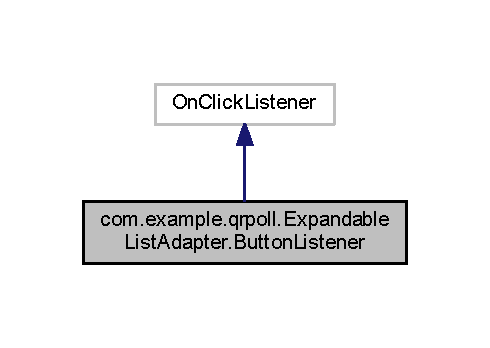
\includegraphics[width=235pt]{classcom_1_1example_1_1qrpoll_1_1_expandable_list_adapter_1_1_button_listener__inherit__graph}
\end{center}
\end{figure}


Diagram współpracy dla com.\+example.\+qrpoll.\+Expandable\+List\+Adapter.\+Button\+Listener\+:\nopagebreak
\begin{figure}[H]
\begin{center}
\leavevmode
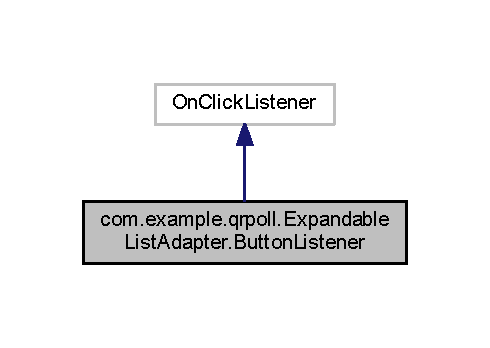
\includegraphics[width=235pt]{classcom_1_1example_1_1qrpoll_1_1_expandable_list_adapter_1_1_button_listener__coll__graph}
\end{center}
\end{figure}
\subsection*{Metody publiczne}
\begin{DoxyCompactItemize}
\item 
void \hyperlink{classcom_1_1example_1_1qrpoll_1_1_expandable_list_adapter_1_1_button_listener_ad69b9ff638eb72e0c337f01955202dc6}{on\+Click} (View arg0)
\end{DoxyCompactItemize}


\subsection{Opis szczegółowy}
Klasa implementujaca on\+Click\+Listner, sluzy do przypisanie akcji pod przyciski do wysylania odpowiedzi 

Definicja w linii 203 pliku Expandable\+List\+Adapter.\+java.



\subsection{Dokumentacja funkcji składowych}
\hypertarget{classcom_1_1example_1_1qrpoll_1_1_expandable_list_adapter_1_1_button_listener_ad69b9ff638eb72e0c337f01955202dc6}{\index{com\+::example\+::qrpoll\+::\+Expandable\+List\+Adapter\+::\+Button\+Listener@{com\+::example\+::qrpoll\+::\+Expandable\+List\+Adapter\+::\+Button\+Listener}!on\+Click@{on\+Click}}
\index{on\+Click@{on\+Click}!com\+::example\+::qrpoll\+::\+Expandable\+List\+Adapter\+::\+Button\+Listener@{com\+::example\+::qrpoll\+::\+Expandable\+List\+Adapter\+::\+Button\+Listener}}
\subsubsection[{on\+Click}]{\setlength{\rightskip}{0pt plus 5cm}void com.\+example.\+qrpoll.\+Expandable\+List\+Adapter.\+Button\+Listener.\+on\+Click (
\begin{DoxyParamCaption}
\item[{View}]{arg0}
\end{DoxyParamCaption}
)}}\label{classcom_1_1example_1_1qrpoll_1_1_expandable_list_adapter_1_1_button_listener_ad69b9ff638eb72e0c337f01955202dc6}
Metoda, ktora reaguje na klikniecie na dany przycisk 

Definicja w linii 208 pliku Expandable\+List\+Adapter.\+java.


\begin{DoxyCode}
208                                        \{
209             List<String>list=mapaButton.get(arg0.getId());
210             \textcolor{keywordflow}{if}(list.size()!=0)\{
211                 String vote=null;
212                 \textcolor{keywordflow}{for}(\textcolor{keywordtype}{int} i=0;i<list.size();i++)\{
213                     String \textcolor{keywordtype}{id}=list.get(i).substring(3);
214                     vote+=\textcolor{keywordtype}{id}+\textcolor{stringliteral}{","};           
215                 \}
216                 vote=vote.substring(4,vote.length()-1);
217             AboutDevice rs=\textcolor{keyword}{new} AboutDevice(\hyperlink{classcom_1_1example_1_1qrpoll_1_1_expandable_list_adapter_a7a712744eebf94bc189b44e5d04ff7da}{\_context});
218             poll.vote(sr.createIdToSend()+\textcolor{stringliteral}{"/"}+vote);
219             \}\textcolor{keywordflow}{else}\{
220                 Toast.makeText(\_context.getApplicationContext(),\textcolor{stringliteral}{"Nic nie wybrano"}, Toast.LENGTH\_SHORT).show
      ();
221             \}
222         \}
\end{DoxyCode}


Dokumentacja dla tej klasy została wygenerowana z pliku\+:\begin{DoxyCompactItemize}
\item 
C\+:/\+Users/\+Wodzu/\+Documents/\+Git\+Hub/\+Projekt\+Zespolowy/\+Android Final + dokumentacja/android/qrpoll/src/com/example/qrpoll/\hyperlink{_expandable_list_adapter_8java}{Expandable\+List\+Adapter.\+java}\end{DoxyCompactItemize}

\hypertarget{classcom_1_1example_1_1qrpoll_1_1_choice}{\section{Dokumentacja klasy com.\+example.\+qrpoll.\+Choice}
\label{classcom_1_1example_1_1qrpoll_1_1_choice}\index{com.\+example.\+qrpoll.\+Choice@{com.\+example.\+qrpoll.\+Choice}}
}
\subsection*{Metody publiczne}
\begin{DoxyCompactItemize}
\item 
String \hyperlink{classcom_1_1example_1_1qrpoll_1_1_choice_a2baa8eb7cc3e3704f754f7617f37acb8}{get\+Pk} ()
\item 
String \hyperlink{classcom_1_1example_1_1qrpoll_1_1_choice_a8484f80a3cf1b34172b435eb4bc64df7}{get\+Choice\+\_\+text} ()
\item 
int \hyperlink{classcom_1_1example_1_1qrpoll_1_1_choice_a748824dd96616a7dde38645bd80c8faa}{hash\+Code} ()
\item 
boolean \hyperlink{classcom_1_1example_1_1qrpoll_1_1_choice_ad4e5a0f7bb62a19e63fc4600e6d16c67}{equals} (Object obj)
\end{DoxyCompactItemize}
\subsection*{Funkcje pakietu}
\begin{DoxyCompactItemize}
\item 
\hyperlink{classcom_1_1example_1_1qrpoll_1_1_choice_a66024b291117e1d6986ee90f836fd208}{Choice} (String \hyperlink{classcom_1_1example_1_1qrpoll_1_1_choice_a6213ee79d3a08c00ca588b9813b7e912}{pk}, String \hyperlink{classcom_1_1example_1_1qrpoll_1_1_choice_ab336c2005a764a1d28450c206eeb4ed0}{choice\+\_\+text})
\end{DoxyCompactItemize}
\subsection*{Atrybuty prywatne}
\begin{DoxyCompactItemize}
\item 
String \hyperlink{classcom_1_1example_1_1qrpoll_1_1_choice_a6213ee79d3a08c00ca588b9813b7e912}{pk}
\item 
String \hyperlink{classcom_1_1example_1_1qrpoll_1_1_choice_ab336c2005a764a1d28450c206eeb4ed0}{choice\+\_\+text}
\end{DoxyCompactItemize}


\subsection{Opis szczegółowy}
klasa reprezentujaca odpowiedz \begin{DoxyAuthor}{Autor}
Piotrek 
\end{DoxyAuthor}


Definicja w linii 7 pliku Choice.\+java.



\subsection{Dokumentacja konstruktora i destruktora}
\hypertarget{classcom_1_1example_1_1qrpoll_1_1_choice_a66024b291117e1d6986ee90f836fd208}{\index{com\+::example\+::qrpoll\+::\+Choice@{com\+::example\+::qrpoll\+::\+Choice}!Choice@{Choice}}
\index{Choice@{Choice}!com\+::example\+::qrpoll\+::\+Choice@{com\+::example\+::qrpoll\+::\+Choice}}
\subsubsection[{Choice}]{\setlength{\rightskip}{0pt plus 5cm}com.\+example.\+qrpoll.\+Choice.\+Choice (
\begin{DoxyParamCaption}
\item[{String}]{pk, }
\item[{String}]{choice\+\_\+text}
\end{DoxyParamCaption}
)\hspace{0.3cm}{\ttfamily [package]}}}\label{classcom_1_1example_1_1qrpoll_1_1_choice_a66024b291117e1d6986ee90f836fd208}


Definicja w linii 12 pliku Choice.\+java.


\begin{DoxyCode}
12                                          \{
13         this.pk=\hyperlink{classcom_1_1example_1_1qrpoll_1_1_choice_a6213ee79d3a08c00ca588b9813b7e912}{pk};
14         this.choice\_text = \hyperlink{classcom_1_1example_1_1qrpoll_1_1_choice_ab336c2005a764a1d28450c206eeb4ed0}{choice\_text};
15     \}
\end{DoxyCode}


\subsection{Dokumentacja funkcji składowych}
\hypertarget{classcom_1_1example_1_1qrpoll_1_1_choice_ad4e5a0f7bb62a19e63fc4600e6d16c67}{\index{com\+::example\+::qrpoll\+::\+Choice@{com\+::example\+::qrpoll\+::\+Choice}!equals@{equals}}
\index{equals@{equals}!com\+::example\+::qrpoll\+::\+Choice@{com\+::example\+::qrpoll\+::\+Choice}}
\subsubsection[{equals}]{\setlength{\rightskip}{0pt plus 5cm}boolean com.\+example.\+qrpoll.\+Choice.\+equals (
\begin{DoxyParamCaption}
\item[{Object}]{obj}
\end{DoxyParamCaption}
)}}\label{classcom_1_1example_1_1qrpoll_1_1_choice_ad4e5a0f7bb62a19e63fc4600e6d16c67}
metoda porownujaca 2 obiekty typu \hyperlink{classcom_1_1example_1_1qrpoll_1_1_choice}{Choice} 
\begin{DoxyParams}{Parametry}
{\em obj} & obiekt z ktorym bedziemy porownywac \\
\hline
\end{DoxyParams}


Definicja w linii 50 pliku Choice.\+java.


\begin{DoxyCode}
50                                       \{
51         \textcolor{keywordflow}{if} (\textcolor{keyword}{this} == obj)
52             \textcolor{keywordflow}{return} \textcolor{keyword}{true};
53         \textcolor{keywordflow}{if} (obj == null)
54             \textcolor{keywordflow}{return} \textcolor{keyword}{false};
55         \textcolor{keywordflow}{if} (getClass() != obj.getClass())
56             \textcolor{keywordflow}{return} \textcolor{keyword}{false};
57         \hyperlink{classcom_1_1example_1_1qrpoll_1_1_choice_a66024b291117e1d6986ee90f836fd208}{Choice} other = (\hyperlink{classcom_1_1example_1_1qrpoll_1_1_choice_a66024b291117e1d6986ee90f836fd208}{Choice}) obj;
58         \textcolor{keywordflow}{if} (\hyperlink{classcom_1_1example_1_1qrpoll_1_1_choice_ab336c2005a764a1d28450c206eeb4ed0}{choice\_text} == null) \{
59             \textcolor{keywordflow}{if} (other.choice\_text != null)
60                 \textcolor{keywordflow}{return} \textcolor{keyword}{false};
61         \} \textcolor{keywordflow}{else} \textcolor{keywordflow}{if} (!\hyperlink{classcom_1_1example_1_1qrpoll_1_1_choice_ab336c2005a764a1d28450c206eeb4ed0}{choice\_text}.equals(other.choice\_text))
62             \textcolor{keywordflow}{return} \textcolor{keyword}{false};
63         \textcolor{keywordflow}{if} (\hyperlink{classcom_1_1example_1_1qrpoll_1_1_choice_a6213ee79d3a08c00ca588b9813b7e912}{pk} == null) \{
64             \textcolor{keywordflow}{if} (other.pk != null)
65                 \textcolor{keywordflow}{return} \textcolor{keyword}{false};
66         \} \textcolor{keywordflow}{else} \textcolor{keywordflow}{if} (!\hyperlink{classcom_1_1example_1_1qrpoll_1_1_choice_a6213ee79d3a08c00ca588b9813b7e912}{pk}.equals(other.pk))
67             \textcolor{keywordflow}{return} \textcolor{keyword}{false};
68         
69         \textcolor{keywordflow}{return} \textcolor{keyword}{true};
70     \}
\end{DoxyCode}
\hypertarget{classcom_1_1example_1_1qrpoll_1_1_choice_a8484f80a3cf1b34172b435eb4bc64df7}{\index{com\+::example\+::qrpoll\+::\+Choice@{com\+::example\+::qrpoll\+::\+Choice}!get\+Choice\+\_\+text@{get\+Choice\+\_\+text}}
\index{get\+Choice\+\_\+text@{get\+Choice\+\_\+text}!com\+::example\+::qrpoll\+::\+Choice@{com\+::example\+::qrpoll\+::\+Choice}}
\subsubsection[{get\+Choice\+\_\+text}]{\setlength{\rightskip}{0pt plus 5cm}String com.\+example.\+qrpoll.\+Choice.\+get\+Choice\+\_\+text (
\begin{DoxyParamCaption}
{}
\end{DoxyParamCaption}
)}}\label{classcom_1_1example_1_1qrpoll_1_1_choice_a8484f80a3cf1b34172b435eb4bc64df7}
\begin{DoxyReturn}{Zwraca}
tresc odpowiedzi 
\end{DoxyReturn}


Definicja w linii 27 pliku Choice.\+java.


\begin{DoxyCode}
27                                    \{
28         \textcolor{keywordflow}{return} \hyperlink{classcom_1_1example_1_1qrpoll_1_1_choice_ab336c2005a764a1d28450c206eeb4ed0}{choice\_text};
29     \}
\end{DoxyCode}
\hypertarget{classcom_1_1example_1_1qrpoll_1_1_choice_a2baa8eb7cc3e3704f754f7617f37acb8}{\index{com\+::example\+::qrpoll\+::\+Choice@{com\+::example\+::qrpoll\+::\+Choice}!get\+Pk@{get\+Pk}}
\index{get\+Pk@{get\+Pk}!com\+::example\+::qrpoll\+::\+Choice@{com\+::example\+::qrpoll\+::\+Choice}}
\subsubsection[{get\+Pk}]{\setlength{\rightskip}{0pt plus 5cm}String com.\+example.\+qrpoll.\+Choice.\+get\+Pk (
\begin{DoxyParamCaption}
{}
\end{DoxyParamCaption}
)}}\label{classcom_1_1example_1_1qrpoll_1_1_choice_a2baa8eb7cc3e3704f754f7617f37acb8}
\begin{DoxyReturn}{Zwraca}
id odpowiedzi 
\end{DoxyReturn}


Definicja w linii 20 pliku Choice.\+java.


\begin{DoxyCode}
20                           \{
21         \textcolor{keywordflow}{return} \hyperlink{classcom_1_1example_1_1qrpoll_1_1_choice_a6213ee79d3a08c00ca588b9813b7e912}{pk};
22     \}
\end{DoxyCode}
\hypertarget{classcom_1_1example_1_1qrpoll_1_1_choice_a748824dd96616a7dde38645bd80c8faa}{\index{com\+::example\+::qrpoll\+::\+Choice@{com\+::example\+::qrpoll\+::\+Choice}!hash\+Code@{hash\+Code}}
\index{hash\+Code@{hash\+Code}!com\+::example\+::qrpoll\+::\+Choice@{com\+::example\+::qrpoll\+::\+Choice}}
\subsubsection[{hash\+Code}]{\setlength{\rightskip}{0pt plus 5cm}int com.\+example.\+qrpoll.\+Choice.\+hash\+Code (
\begin{DoxyParamCaption}
{}
\end{DoxyParamCaption}
)}}\label{classcom_1_1example_1_1qrpoll_1_1_choice_a748824dd96616a7dde38645bd80c8faa}
metoda obliczajace kod hash 

Definicja w linii 35 pliku Choice.\+java.


\begin{DoxyCode}
35                           \{
36         \textcolor{keyword}{final} \textcolor{keywordtype}{int} prime = 31;
37         \textcolor{keywordtype}{int} result = 1;
38         result = prime * result
39                 + ((\hyperlink{classcom_1_1example_1_1qrpoll_1_1_choice_ab336c2005a764a1d28450c206eeb4ed0}{choice\_text} == null) ? 0 : choice\_text.hashCode());
40         result = prime * result + ((\hyperlink{classcom_1_1example_1_1qrpoll_1_1_choice_a6213ee79d3a08c00ca588b9813b7e912}{pk} == null) ? 0 : pk.hashCode());
41         result = prime * result ;
42         \textcolor{keywordflow}{return} result;
43     \}
\end{DoxyCode}


\subsection{Dokumentacja atrybutów składowych}
\hypertarget{classcom_1_1example_1_1qrpoll_1_1_choice_ab336c2005a764a1d28450c206eeb4ed0}{\index{com\+::example\+::qrpoll\+::\+Choice@{com\+::example\+::qrpoll\+::\+Choice}!choice\+\_\+text@{choice\+\_\+text}}
\index{choice\+\_\+text@{choice\+\_\+text}!com\+::example\+::qrpoll\+::\+Choice@{com\+::example\+::qrpoll\+::\+Choice}}
\subsubsection[{choice\+\_\+text}]{\setlength{\rightskip}{0pt plus 5cm}String com.\+example.\+qrpoll.\+Choice.\+choice\+\_\+text\hspace{0.3cm}{\ttfamily [private]}}}\label{classcom_1_1example_1_1qrpoll_1_1_choice_ab336c2005a764a1d28450c206eeb4ed0}


Definicja w linii 10 pliku Choice.\+java.

\hypertarget{classcom_1_1example_1_1qrpoll_1_1_choice_a6213ee79d3a08c00ca588b9813b7e912}{\index{com\+::example\+::qrpoll\+::\+Choice@{com\+::example\+::qrpoll\+::\+Choice}!pk@{pk}}
\index{pk@{pk}!com\+::example\+::qrpoll\+::\+Choice@{com\+::example\+::qrpoll\+::\+Choice}}
\subsubsection[{pk}]{\setlength{\rightskip}{0pt plus 5cm}String com.\+example.\+qrpoll.\+Choice.\+pk\hspace{0.3cm}{\ttfamily [private]}}}\label{classcom_1_1example_1_1qrpoll_1_1_choice_a6213ee79d3a08c00ca588b9813b7e912}


Definicja w linii 9 pliku Choice.\+java.



Dokumentacja dla tej klasy została wygenerowana z pliku\+:\begin{DoxyCompactItemize}
\item 
\hyperlink{_choice_8java}{Choice.\+java}\end{DoxyCompactItemize}

\hypertarget{classcom_1_1example_1_1qrpoll_1_1_sql_handler_1_1_database_helper}{\section{Dokumentacja klasy com.\+example.\+qrpoll.\+Sql\+Handler.\+Database\+Helper}
\label{classcom_1_1example_1_1qrpoll_1_1_sql_handler_1_1_database_helper}\index{com.\+example.\+qrpoll.\+Sql\+Handler.\+Database\+Helper@{com.\+example.\+qrpoll.\+Sql\+Handler.\+Database\+Helper}}
}


Diagram dziedziczenia dla com.\+example.\+qrpoll.\+Sql\+Handler.\+Database\+Helper
\nopagebreak
\begin{figure}[H]
\begin{center}
\leavevmode
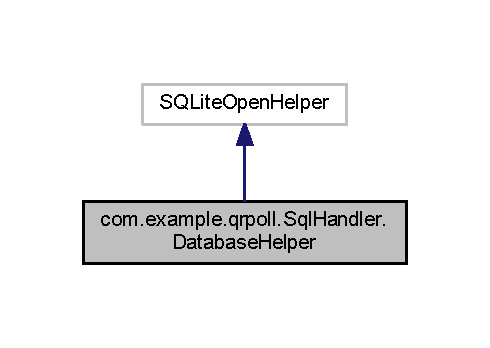
\includegraphics[width=235pt]{classcom_1_1example_1_1qrpoll_1_1_sql_handler_1_1_database_helper__inherit__graph}
\end{center}
\end{figure}


Diagram współpracy dla com.\+example.\+qrpoll.\+Sql\+Handler.\+Database\+Helper\+:
\nopagebreak
\begin{figure}[H]
\begin{center}
\leavevmode
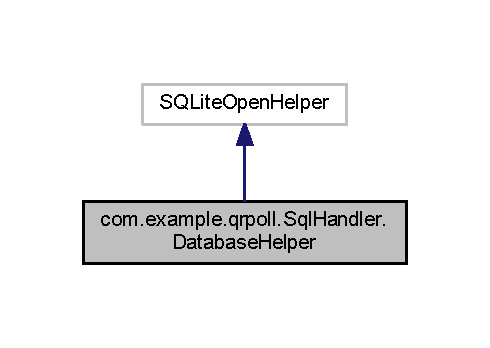
\includegraphics[width=235pt]{classcom_1_1example_1_1qrpoll_1_1_sql_handler_1_1_database_helper__coll__graph}
\end{center}
\end{figure}
\subsection*{Metody publiczne}
\begin{DoxyCompactItemize}
\item 
\hyperlink{classcom_1_1example_1_1qrpoll_1_1_sql_handler_1_1_database_helper_a7ed7b7a35028af5444c25739c1883f6b}{Database\+Helper} (Context \hyperlink{classcom_1_1example_1_1qrpoll_1_1_sql_handler_ab0071f750233a8b37790758a430d847c}{context}, String name, Cursor\+Factory factory, int version)
\item 
void \hyperlink{classcom_1_1example_1_1qrpoll_1_1_sql_handler_1_1_database_helper_a8165a214907379c8e6c7548aa51f3e01}{on\+Create} (S\+Q\+Lite\+Database \hyperlink{classcom_1_1example_1_1qrpoll_1_1_sql_handler_a5b422e7952698eb1df158709d4e18007}{db})
\item 
void \hyperlink{classcom_1_1example_1_1qrpoll_1_1_sql_handler_1_1_database_helper_a66f602b9f661c21a224d97c2bbfc257a}{on\+Upgrade} (S\+Q\+Lite\+Database arg0, int arg1, int arg2)
\end{DoxyCompactItemize}


\subsection{Opis szczegółowy}
pomocnicza klasa do tworzenia bazy danych \begin{DoxyAuthor}{Autor}
wodzu 
\end{DoxyAuthor}


Definicja w linii 150 pliku Sql\+Handler.\+java.



\subsection{Dokumentacja konstruktora i destruktora}
\hypertarget{classcom_1_1example_1_1qrpoll_1_1_sql_handler_1_1_database_helper_a7ed7b7a35028af5444c25739c1883f6b}{\index{com\+::example\+::qrpoll\+::\+Sql\+Handler\+::\+Database\+Helper@{com\+::example\+::qrpoll\+::\+Sql\+Handler\+::\+Database\+Helper}!Database\+Helper@{Database\+Helper}}
\index{Database\+Helper@{Database\+Helper}!com\+::example\+::qrpoll\+::\+Sql\+Handler\+::\+Database\+Helper@{com\+::example\+::qrpoll\+::\+Sql\+Handler\+::\+Database\+Helper}}
\subsubsection[{Database\+Helper}]{\setlength{\rightskip}{0pt plus 5cm}com.\+example.\+qrpoll.\+Sql\+Handler.\+Database\+Helper.\+Database\+Helper (
\begin{DoxyParamCaption}
\item[{Context}]{context, }
\item[{String}]{name, }
\item[{Cursor\+Factory}]{factory, }
\item[{int}]{version}
\end{DoxyParamCaption}
)}}\label{classcom_1_1example_1_1qrpoll_1_1_sql_handler_1_1_database_helper_a7ed7b7a35028af5444c25739c1883f6b}

\begin{DoxyParams}{Parametry}
{\em context} & \\
\hline
{\em name} & \\
\hline
{\em factory} & \\
\hline
{\em version} & \\
\hline
\end{DoxyParams}


Definicja w linii 158 pliku Sql\+Handler.\+java.


\begin{DoxyCode}
158                                                                                                 \{
159                 super(\hyperlink{classcom_1_1example_1_1qrpoll_1_1_sql_handler_ab0071f750233a8b37790758a430d847c}{context},name,factory,version);
160             \}
\end{DoxyCode}


\subsection{Dokumentacja funkcji składowych}
\hypertarget{classcom_1_1example_1_1qrpoll_1_1_sql_handler_1_1_database_helper_a8165a214907379c8e6c7548aa51f3e01}{\index{com\+::example\+::qrpoll\+::\+Sql\+Handler\+::\+Database\+Helper@{com\+::example\+::qrpoll\+::\+Sql\+Handler\+::\+Database\+Helper}!on\+Create@{on\+Create}}
\index{on\+Create@{on\+Create}!com\+::example\+::qrpoll\+::\+Sql\+Handler\+::\+Database\+Helper@{com\+::example\+::qrpoll\+::\+Sql\+Handler\+::\+Database\+Helper}}
\subsubsection[{on\+Create}]{\setlength{\rightskip}{0pt plus 5cm}void com.\+example.\+qrpoll.\+Sql\+Handler.\+Database\+Helper.\+on\+Create (
\begin{DoxyParamCaption}
\item[{S\+Q\+Lite\+Database}]{db}
\end{DoxyParamCaption}
)}}\label{classcom_1_1example_1_1qrpoll_1_1_sql_handler_1_1_database_helper_a8165a214907379c8e6c7548aa51f3e01}
tworzenie bazy danych 

Definicja w linii 165 pliku Sql\+Handler.\+java.


\begin{DoxyCode}
165                                                     \{
166                 db.execSQL(\hyperlink{classcom_1_1example_1_1qrpoll_1_1_sql_handler_a41cc7444128cfe954cd829ceb98d8df0}{Create\_table\_spotkania});
167                 Log.d(\textcolor{stringliteral}{"SqLiteTodoManager"}, \textcolor{stringliteral}{"Database creating..."});
168             \}
\end{DoxyCode}
\hypertarget{classcom_1_1example_1_1qrpoll_1_1_sql_handler_1_1_database_helper_a66f602b9f661c21a224d97c2bbfc257a}{\index{com\+::example\+::qrpoll\+::\+Sql\+Handler\+::\+Database\+Helper@{com\+::example\+::qrpoll\+::\+Sql\+Handler\+::\+Database\+Helper}!on\+Upgrade@{on\+Upgrade}}
\index{on\+Upgrade@{on\+Upgrade}!com\+::example\+::qrpoll\+::\+Sql\+Handler\+::\+Database\+Helper@{com\+::example\+::qrpoll\+::\+Sql\+Handler\+::\+Database\+Helper}}
\subsubsection[{on\+Upgrade}]{\setlength{\rightskip}{0pt plus 5cm}void com.\+example.\+qrpoll.\+Sql\+Handler.\+Database\+Helper.\+on\+Upgrade (
\begin{DoxyParamCaption}
\item[{S\+Q\+Lite\+Database}]{arg0, }
\item[{int}]{arg1, }
\item[{int}]{arg2}
\end{DoxyParamCaption}
)}}\label{classcom_1_1example_1_1qrpoll_1_1_sql_handler_1_1_database_helper_a66f602b9f661c21a224d97c2bbfc257a}
update krotek (nie zaimplementowano) 

Definicja w linii 173 pliku Sql\+Handler.\+java.


\begin{DoxyCode}
173                                                                            \{
174                 \textcolor{comment}{// TODO Auto-generated method stub}
175                 
176             \}
\end{DoxyCode}


Dokumentacja dla tej klasy została wygenerowana z pliku\+:\begin{DoxyCompactItemize}
\item 
\hyperlink{_sql_handler_8java}{Sql\+Handler.\+java}\end{DoxyCompactItemize}

\hypertarget{classcom_1_1example_1_1qrpoll_1_1_exception404}{\section{Dokumentacja klasy com.\+example.\+qrpoll.\+Exception404}
\label{classcom_1_1example_1_1qrpoll_1_1_exception404}\index{com.\+example.\+qrpoll.\+Exception404@{com.\+example.\+qrpoll.\+Exception404}}
}


Diagram dziedziczenia dla com.\+example.\+qrpoll.\+Exception404\nopagebreak
\begin{figure}[H]
\begin{center}
\leavevmode
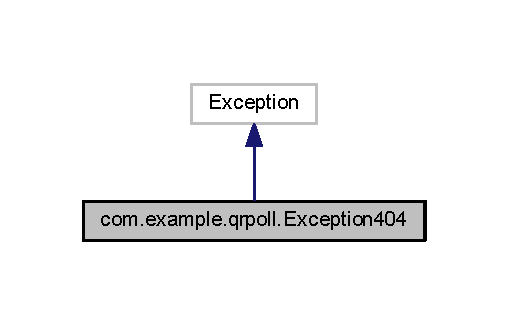
\includegraphics[width=244pt]{classcom_1_1example_1_1qrpoll_1_1_exception404__inherit__graph}
\end{center}
\end{figure}


Diagram współpracy dla com.\+example.\+qrpoll.\+Exception404\+:\nopagebreak
\begin{figure}[H]
\begin{center}
\leavevmode
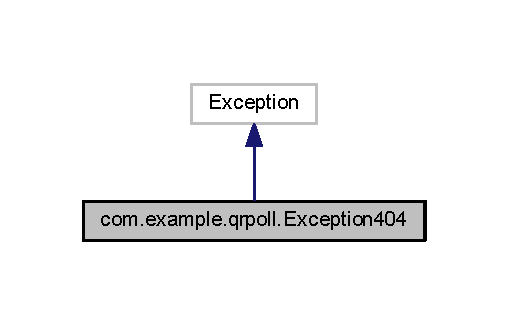
\includegraphics[width=244pt]{classcom_1_1example_1_1qrpoll_1_1_exception404__coll__graph}
\end{center}
\end{figure}
\subsection*{Funkcje pakietu}
\begin{DoxyCompactItemize}
\item 
\hyperlink{classcom_1_1example_1_1qrpoll_1_1_exception404_a8927591383f273a89d49e4bf6f536961}{Exception404} ()
\end{DoxyCompactItemize}


\subsection{Opis szczegółowy}
wyjatek w wypadku, gdy serwer nie moze polaczyc sie z danym url 

Definicja w linii 15 pliku Exception404.\+java.



\subsection{Dokumentacja konstruktora i destruktora}
\hypertarget{classcom_1_1example_1_1qrpoll_1_1_exception404_a8927591383f273a89d49e4bf6f536961}{\index{com\+::example\+::qrpoll\+::\+Exception404@{com\+::example\+::qrpoll\+::\+Exception404}!Exception404@{Exception404}}
\index{Exception404@{Exception404}!com\+::example\+::qrpoll\+::\+Exception404@{com\+::example\+::qrpoll\+::\+Exception404}}
\subsubsection[{Exception404}]{\setlength{\rightskip}{0pt plus 5cm}com.\+example.\+qrpoll.\+Exception404.\+Exception404 (
\begin{DoxyParamCaption}
{}
\end{DoxyParamCaption}
)\hspace{0.3cm}{\ttfamily [package]}}}\label{classcom_1_1example_1_1qrpoll_1_1_exception404_a8927591383f273a89d49e4bf6f536961}


Definicja w linii 16 pliku Exception404.\+java.


\begin{DoxyCode}
16                   \{
17         super();
18     \}
\end{DoxyCode}


Dokumentacja dla tej klasy została wygenerowana z pliku\+:\begin{DoxyCompactItemize}
\item 
C\+:/\+Users/\+Wodzu/\+Documents/\+Git\+Hub/\+Projekt\+Zespolowy/\+Android Final + dokumentacja/android/qrpoll/src/com/example/qrpoll/\hyperlink{_exception404_8java}{Exception404.\+java}\end{DoxyCompactItemize}

\hypertarget{classcom_1_1example_1_1qrpoll_1_1_expandable_list_adapter}{\section{Dokumentacja klasy com.\+example.\+qrpoll.\+Expandable\+List\+Adapter}
\label{classcom_1_1example_1_1qrpoll_1_1_expandable_list_adapter}\index{com.\+example.\+qrpoll.\+Expandable\+List\+Adapter@{com.\+example.\+qrpoll.\+Expandable\+List\+Adapter}}
}


Diagram dziedziczenia dla com.\+example.\+qrpoll.\+Expandable\+List\+Adapter
\nopagebreak
\begin{figure}[H]
\begin{center}
\leavevmode
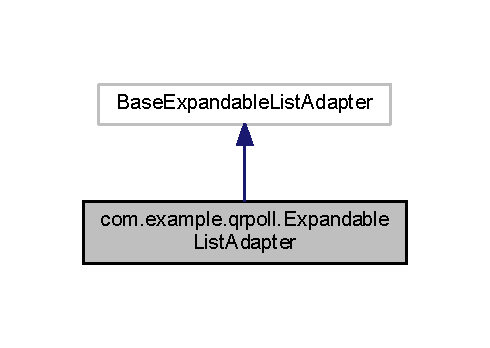
\includegraphics[width=235pt]{classcom_1_1example_1_1qrpoll_1_1_expandable_list_adapter__inherit__graph}
\end{center}
\end{figure}


Diagram współpracy dla com.\+example.\+qrpoll.\+Expandable\+List\+Adapter\+:
\nopagebreak
\begin{figure}[H]
\begin{center}
\leavevmode
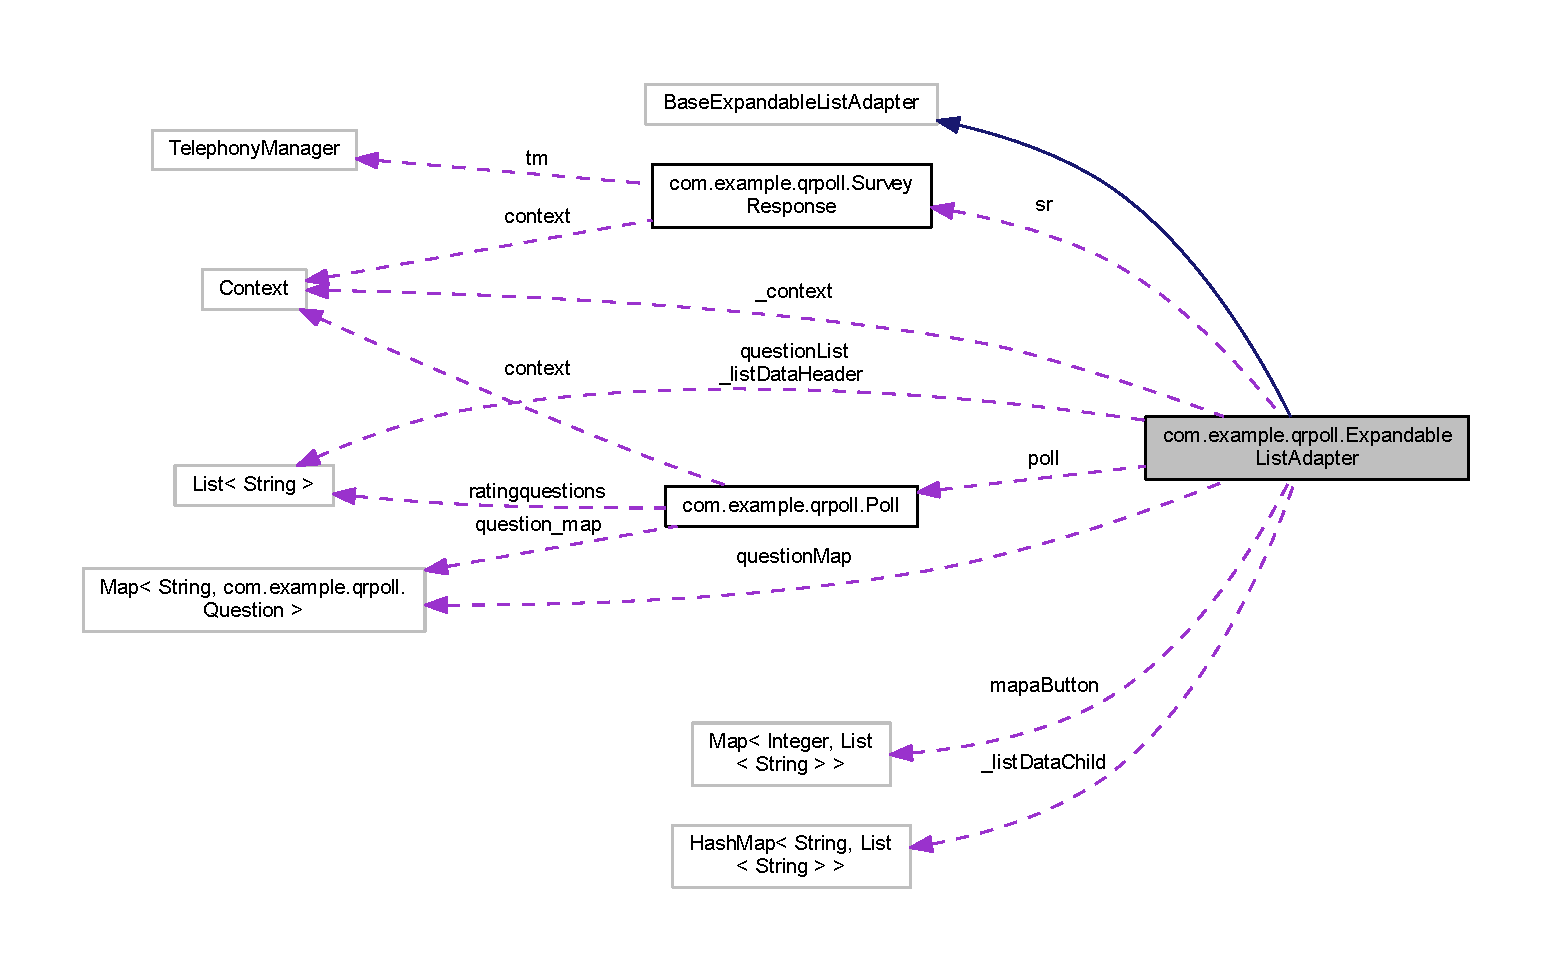
\includegraphics[width=350pt]{classcom_1_1example_1_1qrpoll_1_1_expandable_list_adapter__coll__graph}
\end{center}
\end{figure}
\subsection*{Komponenty}
\begin{DoxyCompactItemize}
\item 
class \hyperlink{classcom_1_1example_1_1qrpoll_1_1_expandable_list_adapter_1_1_button_listener}{Button\+Listener}
\end{DoxyCompactItemize}
\subsection*{Metody publiczne}
\begin{DoxyCompactItemize}
\item 
void \hyperlink{classcom_1_1example_1_1qrpoll_1_1_expandable_list_adapter_a8124339d7fc7169df890068e07c76e41}{set\+Questions} ()
\item 
void \hyperlink{classcom_1_1example_1_1qrpoll_1_1_expandable_list_adapter_a76c2b3720ad077a33ac32cb371aea902}{set\+Poll} (\hyperlink{classcom_1_1example_1_1qrpoll_1_1_poll}{Poll} \hyperlink{classcom_1_1example_1_1qrpoll_1_1_expandable_list_adapter_a35f2a91149fc7265646cd916c54a02ef}{poll})
\item 
\hyperlink{classcom_1_1example_1_1qrpoll_1_1_expandable_list_adapter_af5cff710db9f2515f997f24bb1b2d816}{Expandable\+List\+Adapter} (Context context, List$<$ String $>$ list\+Data\+Header, Hash\+Map$<$ String, List$<$ String $>$$>$ list\+Child\+Data, \hyperlink{classcom_1_1example_1_1qrpoll_1_1_poll}{Poll} \hyperlink{classcom_1_1example_1_1qrpoll_1_1_expandable_list_adapter_a35f2a91149fc7265646cd916c54a02ef}{poll})
\item 
Object \hyperlink{classcom_1_1example_1_1qrpoll_1_1_expandable_list_adapter_a85fb08a976c8961e0f3e9fed7eae064e}{get\+Child} (int group\+Position, int child\+Posititon)
\item 
long \hyperlink{classcom_1_1example_1_1qrpoll_1_1_expandable_list_adapter_a34e4958bd1ff0cc578cb8c65b26d4d4b}{get\+Child\+Id} (int group\+Position, int child\+Position)
\item 
View \hyperlink{classcom_1_1example_1_1qrpoll_1_1_expandable_list_adapter_a4d933f905a39d145b9e400693dc90193}{get\+Child\+View} (final int group\+Position, final int child\+Position, boolean is\+Last\+Child, View convert\+View, View\+Group parent)
\item 
int \hyperlink{classcom_1_1example_1_1qrpoll_1_1_expandable_list_adapter_abd5d4f934326b8ec5ea92580d81e5616}{get\+Children\+Count} (int group\+Position)
\item 
Object \hyperlink{classcom_1_1example_1_1qrpoll_1_1_expandable_list_adapter_a3f311ecc161915f1d8a864677d36b752}{get\+Group} (int group\+Position)
\item 
int \hyperlink{classcom_1_1example_1_1qrpoll_1_1_expandable_list_adapter_ab9a9bd19ec9d4209100f8d08b56b2837}{get\+Group\+Count} ()
\item 
long \hyperlink{classcom_1_1example_1_1qrpoll_1_1_expandable_list_adapter_a9e1426065947818273f73aca8a592239}{get\+Group\+Id} (int group\+Position)
\item 
View \hyperlink{classcom_1_1example_1_1qrpoll_1_1_expandable_list_adapter_a6b8e4143490f8afe57b71a6c8ab2b0a4}{get\+Group\+View} (int group\+Position, boolean is\+Expanded, View convert\+View, View\+Group parent)
\item 
boolean \hyperlink{classcom_1_1example_1_1qrpoll_1_1_expandable_list_adapter_a57e5cc39a98135f8082d543188b916ba}{has\+Stable\+Ids} ()
\item 
boolean \hyperlink{classcom_1_1example_1_1qrpoll_1_1_expandable_list_adapter_af45bff70a6085ba623e21e42116c5275}{is\+Child\+Selectable} (int group\+Position, int child\+Position)
\end{DoxyCompactItemize}
\subsection*{Atrybuty publiczne}
\begin{DoxyCompactItemize}
\item 
\hyperlink{classcom_1_1example_1_1qrpoll_1_1_survey_response}{Survey\+Response} \hyperlink{classcom_1_1example_1_1qrpoll_1_1_expandable_list_adapter_a38af3904440bf552715d92f8c6e1375d}{sr}
\end{DoxyCompactItemize}
\subsection*{Atrybuty prywatne}
\begin{DoxyCompactItemize}
\item 
Context \hyperlink{classcom_1_1example_1_1qrpoll_1_1_expandable_list_adapter_a7a712744eebf94bc189b44e5d04ff7da}{\+\_\+context}
\item 
\hyperlink{classcom_1_1example_1_1qrpoll_1_1_poll}{Poll} \hyperlink{classcom_1_1example_1_1qrpoll_1_1_expandable_list_adapter_a35f2a91149fc7265646cd916c54a02ef}{poll}
\item 
Map$<$ String, \hyperlink{classcom_1_1example_1_1qrpoll_1_1_question}{Question} $>$ \hyperlink{classcom_1_1example_1_1qrpoll_1_1_expandable_list_adapter_a5ec37e3c4af51739b2c0cd282b9bf208}{question\+Map}
\item 
Map$<$ Integer, List$<$ String $>$ $>$ \hyperlink{classcom_1_1example_1_1qrpoll_1_1_expandable_list_adapter_a8351d33fae079b02fb540090d49c6f2e}{mapa\+Button}
\item 
List$<$ String $>$ \hyperlink{classcom_1_1example_1_1qrpoll_1_1_expandable_list_adapter_a21519cda6be88f0b729afc1ac0cc06a5}{question\+List}
\item 
List$<$ String $>$ \hyperlink{classcom_1_1example_1_1qrpoll_1_1_expandable_list_adapter_a7290d1e184f1a8ef03ad8ea5bd4f273d}{\+\_\+list\+Data\+Header}
\item 
Hash\+Map$<$ String, List$<$ String $>$ $>$ \hyperlink{classcom_1_1example_1_1qrpoll_1_1_expandable_list_adapter_a9e3d05b47021b43ad465a1f7fa3d0ca2}{\+\_\+list\+Data\+Child}
\end{DoxyCompactItemize}


\subsection{Opis szczegółowy}
klasa adaptera do listy z pytaniami 

Definicja w linii 28 pliku Expandable\+List\+Adapter.\+java.



\subsection{Dokumentacja konstruktora i destruktora}
\hypertarget{classcom_1_1example_1_1qrpoll_1_1_expandable_list_adapter_af5cff710db9f2515f997f24bb1b2d816}{\index{com\+::example\+::qrpoll\+::\+Expandable\+List\+Adapter@{com\+::example\+::qrpoll\+::\+Expandable\+List\+Adapter}!Expandable\+List\+Adapter@{Expandable\+List\+Adapter}}
\index{Expandable\+List\+Adapter@{Expandable\+List\+Adapter}!com\+::example\+::qrpoll\+::\+Expandable\+List\+Adapter@{com\+::example\+::qrpoll\+::\+Expandable\+List\+Adapter}}
\subsubsection[{Expandable\+List\+Adapter}]{\setlength{\rightskip}{0pt plus 5cm}com.\+example.\+qrpoll.\+Expandable\+List\+Adapter.\+Expandable\+List\+Adapter (
\begin{DoxyParamCaption}
\item[{Context}]{context, }
\item[{List$<$ String $>$}]{list\+Data\+Header, }
\item[{Hash\+Map$<$ String, List$<$ String $>$$>$}]{list\+Child\+Data, }
\item[{{\bf Poll}}]{poll}
\end{DoxyParamCaption}
)}}\label{classcom_1_1example_1_1qrpoll_1_1_expandable_list_adapter_af5cff710db9f2515f997f24bb1b2d816}


Definicja w linii 58 pliku Expandable\+List\+Adapter.\+java.


\begin{DoxyCode}
59                                                                    \{
60         this.\_context = context;
61         this.\_listDataHeader = listDataHeader;
62         this.\_listDataChild = listChildData;
63         \hyperlink{classcom_1_1example_1_1qrpoll_1_1_expandable_list_adapter_a38af3904440bf552715d92f8c6e1375d}{sr}=\textcolor{keyword}{new} SurveyResponse(context);
64         \hyperlink{classcom_1_1example_1_1qrpoll_1_1_expandable_list_adapter_a8351d33fae079b02fb540090d49c6f2e}{mapaButton}=\textcolor{keyword}{new} HashMap<Integer,List<String>>();
65         \hyperlink{classcom_1_1example_1_1qrpoll_1_1_expandable_list_adapter_a76c2b3720ad077a33ac32cb371aea902}{setPoll}(\hyperlink{classcom_1_1example_1_1qrpoll_1_1_expandable_list_adapter_a35f2a91149fc7265646cd916c54a02ef}{poll});
66         \hyperlink{classcom_1_1example_1_1qrpoll_1_1_expandable_list_adapter_a8124339d7fc7169df890068e07c76e41}{setQuestions}();
67     \}
\end{DoxyCode}


\subsection{Dokumentacja funkcji składowych}
\hypertarget{classcom_1_1example_1_1qrpoll_1_1_expandable_list_adapter_a85fb08a976c8961e0f3e9fed7eae064e}{\index{com\+::example\+::qrpoll\+::\+Expandable\+List\+Adapter@{com\+::example\+::qrpoll\+::\+Expandable\+List\+Adapter}!get\+Child@{get\+Child}}
\index{get\+Child@{get\+Child}!com\+::example\+::qrpoll\+::\+Expandable\+List\+Adapter@{com\+::example\+::qrpoll\+::\+Expandable\+List\+Adapter}}
\subsubsection[{get\+Child}]{\setlength{\rightskip}{0pt plus 5cm}Object com.\+example.\+qrpoll.\+Expandable\+List\+Adapter.\+get\+Child (
\begin{DoxyParamCaption}
\item[{int}]{group\+Position, }
\item[{int}]{child\+Posititon}
\end{DoxyParamCaption}
)}}\label{classcom_1_1example_1_1qrpoll_1_1_expandable_list_adapter_a85fb08a976c8961e0f3e9fed7eae064e}


Definicja w linii 70 pliku Expandable\+List\+Adapter.\+java.


\begin{DoxyCode}
70                                                                   \{
71         \textcolor{keywordflow}{return} this.\_listDataChild.get(this.\_listDataHeader.get(groupPosition))
72                 .get(childPosititon);
73     \}
\end{DoxyCode}
\hypertarget{classcom_1_1example_1_1qrpoll_1_1_expandable_list_adapter_a34e4958bd1ff0cc578cb8c65b26d4d4b}{\index{com\+::example\+::qrpoll\+::\+Expandable\+List\+Adapter@{com\+::example\+::qrpoll\+::\+Expandable\+List\+Adapter}!get\+Child\+Id@{get\+Child\+Id}}
\index{get\+Child\+Id@{get\+Child\+Id}!com\+::example\+::qrpoll\+::\+Expandable\+List\+Adapter@{com\+::example\+::qrpoll\+::\+Expandable\+List\+Adapter}}
\subsubsection[{get\+Child\+Id}]{\setlength{\rightskip}{0pt plus 5cm}long com.\+example.\+qrpoll.\+Expandable\+List\+Adapter.\+get\+Child\+Id (
\begin{DoxyParamCaption}
\item[{int}]{group\+Position, }
\item[{int}]{child\+Position}
\end{DoxyParamCaption}
)}}\label{classcom_1_1example_1_1qrpoll_1_1_expandable_list_adapter_a34e4958bd1ff0cc578cb8c65b26d4d4b}


Definicja w linii 76 pliku Expandable\+List\+Adapter.\+java.


\begin{DoxyCode}
76                                                                  \{
77         \textcolor{keywordflow}{return} childPosition;
78     \}
\end{DoxyCode}
\hypertarget{classcom_1_1example_1_1qrpoll_1_1_expandable_list_adapter_abd5d4f934326b8ec5ea92580d81e5616}{\index{com\+::example\+::qrpoll\+::\+Expandable\+List\+Adapter@{com\+::example\+::qrpoll\+::\+Expandable\+List\+Adapter}!get\+Children\+Count@{get\+Children\+Count}}
\index{get\+Children\+Count@{get\+Children\+Count}!com\+::example\+::qrpoll\+::\+Expandable\+List\+Adapter@{com\+::example\+::qrpoll\+::\+Expandable\+List\+Adapter}}
\subsubsection[{get\+Children\+Count}]{\setlength{\rightskip}{0pt plus 5cm}int com.\+example.\+qrpoll.\+Expandable\+List\+Adapter.\+get\+Children\+Count (
\begin{DoxyParamCaption}
\item[{int}]{group\+Position}
\end{DoxyParamCaption}
)}}\label{classcom_1_1example_1_1qrpoll_1_1_expandable_list_adapter_abd5d4f934326b8ec5ea92580d81e5616}


Definicja w linii 144 pliku Expandable\+List\+Adapter.\+java.


\begin{DoxyCode}
144                                                    \{
145         \textcolor{keywordflow}{return} this.\_listDataChild.get(this.\_listDataHeader.get(groupPosition))
146                 .size();
147     \}
\end{DoxyCode}
\hypertarget{classcom_1_1example_1_1qrpoll_1_1_expandable_list_adapter_a4d933f905a39d145b9e400693dc90193}{\index{com\+::example\+::qrpoll\+::\+Expandable\+List\+Adapter@{com\+::example\+::qrpoll\+::\+Expandable\+List\+Adapter}!get\+Child\+View@{get\+Child\+View}}
\index{get\+Child\+View@{get\+Child\+View}!com\+::example\+::qrpoll\+::\+Expandable\+List\+Adapter@{com\+::example\+::qrpoll\+::\+Expandable\+List\+Adapter}}
\subsubsection[{get\+Child\+View}]{\setlength{\rightskip}{0pt plus 5cm}View com.\+example.\+qrpoll.\+Expandable\+List\+Adapter.\+get\+Child\+View (
\begin{DoxyParamCaption}
\item[{final int}]{group\+Position, }
\item[{final int}]{child\+Position, }
\item[{boolean}]{is\+Last\+Child, }
\item[{View}]{convert\+View, }
\item[{View\+Group}]{parent}
\end{DoxyParamCaption}
)}}\label{classcom_1_1example_1_1qrpoll_1_1_expandable_list_adapter_a4d933f905a39d145b9e400693dc90193}
ustawienie wyswietlania pytan 
\begin{DoxyParams}{Parametry}
{\em group\+Position} & \\
\hline
{\em child\+Position} & \\
\hline
{\em is\+Last\+Child} & \\
\hline
{\em convert\+View} & \\
\hline
{\em parent} & \\
\hline
\end{DoxyParams}
\begin{DoxyReturn}{Zwraca}

\end{DoxyReturn}


Definicja w linii 89 pliku Expandable\+List\+Adapter.\+java.


\begin{DoxyCode}
90                                                                      \{
91         String headerTitle = (String) \hyperlink{classcom_1_1example_1_1qrpoll_1_1_expandable_list_adapter_a3f311ecc161915f1d8a864677d36b752}{getGroup}(groupPosition);
92      
93             String key=questionList.get(groupPosition);
94             Question q=questionMap.get(key);
95             Map<String, Choice> choiceMap= q.getChoice\_map();
96             
97             LayoutInflater infalInflater = (LayoutInflater) this.\hyperlink{classcom_1_1example_1_1qrpoll_1_1_expandable_list_adapter_a7a712744eebf94bc189b44e5d04ff7da}{\_context}
98                     .getSystemService(Context.LAYOUT\_INFLATER\_SERVICE);
99             convertView = infalInflater.inflate(R.layout.list\_item, null);
100             LinearLayout linear = (LinearLayout) convertView
101                     .findViewById(R.id.explinear);
102             LinearLayout l=\textcolor{keyword}{new} LinearLayout(this.\hyperlink{classcom_1_1example_1_1qrpoll_1_1_expandable_list_adapter_a7a712744eebf94bc189b44e5d04ff7da}{\_context});
103             l.setOrientation(LinearLayout.VERTICAL);
104             
105             \textcolor{keyword}{final} ArrayList<String> list = \textcolor{keyword}{new} ArrayList<String>();
106             \textcolor{keywordflow}{for}(String choice: choiceMap.keySet())\{
107                 Choice c = choiceMap.get(choice);
108                 CheckBox rb = \textcolor{keyword}{new} CheckBox(this.\hyperlink{classcom_1_1example_1_1qrpoll_1_1_expandable_list_adapter_a7a712744eebf94bc189b44e5d04ff7da}{\_context});
109                 \textcolor{keyword}{final} \textcolor{keywordtype}{int} rbID = Integer.parseInt(c.getPk());
110                 rb.setText(c.getChoice\_text());
111                 rb.setOnCheckedChangeListener(\textcolor{keyword}{new} OnCheckedChangeListener()
112                 \{
113 
114                     @Override
115                     \textcolor{keyword}{public} \textcolor{keywordtype}{void} onCheckedChanged(CompoundButton arg0,
116                             \textcolor{keywordtype}{boolean} arg1) \{
117                         \textcolor{comment}{//Toast.makeText(\_context,groupPosition+"", Toast.LENGTH\_SHORT).show();}
118                         \textcolor{keywordflow}{if}(list.contains(\textcolor{stringliteral}{"id:"}+rbID))\{
119                             
120                             list.remove(\textcolor{stringliteral}{"id:"}+rbID);
121                         \}\textcolor{keywordflow}{else}\{
122                             list.add(\textcolor{stringliteral}{"id:"}+rbID);
123                         \}
124                         
125                     \}
126 
127                 \});
128                 l.addView(rb);
129             \}
130             mapaButton.put(groupPosition, list);
131             Button rb=\textcolor{keyword}{new} Button(this.\hyperlink{classcom_1_1example_1_1qrpoll_1_1_expandable_list_adapter_a7a712744eebf94bc189b44e5d04ff7da}{\_context});
132             rb.setText(\textcolor{stringliteral}{"Zaglosuj"});
133             rb.setId(groupPosition);
134             rb.setOnClickListener(\textcolor{keyword}{new} ButtonListener());
135             l.addView(rb);
136             
137             linear.addView(l);
138 
139  
140         \textcolor{keywordflow}{return} convertView;
141     \}
\end{DoxyCode}
\hypertarget{classcom_1_1example_1_1qrpoll_1_1_expandable_list_adapter_a3f311ecc161915f1d8a864677d36b752}{\index{com\+::example\+::qrpoll\+::\+Expandable\+List\+Adapter@{com\+::example\+::qrpoll\+::\+Expandable\+List\+Adapter}!get\+Group@{get\+Group}}
\index{get\+Group@{get\+Group}!com\+::example\+::qrpoll\+::\+Expandable\+List\+Adapter@{com\+::example\+::qrpoll\+::\+Expandable\+List\+Adapter}}
\subsubsection[{get\+Group}]{\setlength{\rightskip}{0pt plus 5cm}Object com.\+example.\+qrpoll.\+Expandable\+List\+Adapter.\+get\+Group (
\begin{DoxyParamCaption}
\item[{int}]{group\+Position}
\end{DoxyParamCaption}
)}}\label{classcom_1_1example_1_1qrpoll_1_1_expandable_list_adapter_a3f311ecc161915f1d8a864677d36b752}


Definicja w linii 150 pliku Expandable\+List\+Adapter.\+java.


\begin{DoxyCode}
150                                               \{
151         \textcolor{keywordflow}{return} this.\_listDataHeader.get(groupPosition);
152     \}
\end{DoxyCode}
\hypertarget{classcom_1_1example_1_1qrpoll_1_1_expandable_list_adapter_ab9a9bd19ec9d4209100f8d08b56b2837}{\index{com\+::example\+::qrpoll\+::\+Expandable\+List\+Adapter@{com\+::example\+::qrpoll\+::\+Expandable\+List\+Adapter}!get\+Group\+Count@{get\+Group\+Count}}
\index{get\+Group\+Count@{get\+Group\+Count}!com\+::example\+::qrpoll\+::\+Expandable\+List\+Adapter@{com\+::example\+::qrpoll\+::\+Expandable\+List\+Adapter}}
\subsubsection[{get\+Group\+Count}]{\setlength{\rightskip}{0pt plus 5cm}int com.\+example.\+qrpoll.\+Expandable\+List\+Adapter.\+get\+Group\+Count (
\begin{DoxyParamCaption}
{}
\end{DoxyParamCaption}
)}}\label{classcom_1_1example_1_1qrpoll_1_1_expandable_list_adapter_ab9a9bd19ec9d4209100f8d08b56b2837}


Definicja w linii 155 pliku Expandable\+List\+Adapter.\+java.


\begin{DoxyCode}
155                                \{
156         \textcolor{keywordflow}{return} this.\_listDataHeader.size();
157     \}
\end{DoxyCode}
\hypertarget{classcom_1_1example_1_1qrpoll_1_1_expandable_list_adapter_a9e1426065947818273f73aca8a592239}{\index{com\+::example\+::qrpoll\+::\+Expandable\+List\+Adapter@{com\+::example\+::qrpoll\+::\+Expandable\+List\+Adapter}!get\+Group\+Id@{get\+Group\+Id}}
\index{get\+Group\+Id@{get\+Group\+Id}!com\+::example\+::qrpoll\+::\+Expandable\+List\+Adapter@{com\+::example\+::qrpoll\+::\+Expandable\+List\+Adapter}}
\subsubsection[{get\+Group\+Id}]{\setlength{\rightskip}{0pt plus 5cm}long com.\+example.\+qrpoll.\+Expandable\+List\+Adapter.\+get\+Group\+Id (
\begin{DoxyParamCaption}
\item[{int}]{group\+Position}
\end{DoxyParamCaption}
)}}\label{classcom_1_1example_1_1qrpoll_1_1_expandable_list_adapter_a9e1426065947818273f73aca8a592239}


Definicja w linii 160 pliku Expandable\+List\+Adapter.\+java.


\begin{DoxyCode}
160                                               \{
161         \textcolor{keywordflow}{return} groupPosition;
162     \}
\end{DoxyCode}
\hypertarget{classcom_1_1example_1_1qrpoll_1_1_expandable_list_adapter_a6b8e4143490f8afe57b71a6c8ab2b0a4}{\index{com\+::example\+::qrpoll\+::\+Expandable\+List\+Adapter@{com\+::example\+::qrpoll\+::\+Expandable\+List\+Adapter}!get\+Group\+View@{get\+Group\+View}}
\index{get\+Group\+View@{get\+Group\+View}!com\+::example\+::qrpoll\+::\+Expandable\+List\+Adapter@{com\+::example\+::qrpoll\+::\+Expandable\+List\+Adapter}}
\subsubsection[{get\+Group\+View}]{\setlength{\rightskip}{0pt plus 5cm}View com.\+example.\+qrpoll.\+Expandable\+List\+Adapter.\+get\+Group\+View (
\begin{DoxyParamCaption}
\item[{int}]{group\+Position, }
\item[{boolean}]{is\+Expanded, }
\item[{View}]{convert\+View, }
\item[{View\+Group}]{parent}
\end{DoxyParamCaption}
)}}\label{classcom_1_1example_1_1qrpoll_1_1_expandable_list_adapter_a6b8e4143490f8afe57b71a6c8ab2b0a4}


Definicja w linii 165 pliku Expandable\+List\+Adapter.\+java.


\begin{DoxyCode}
166                                                 \{
167         String headerTitle = (String) \hyperlink{classcom_1_1example_1_1qrpoll_1_1_expandable_list_adapter_a3f311ecc161915f1d8a864677d36b752}{getGroup}(groupPosition);
168         \textcolor{keywordflow}{if} (convertView == null) \{
169             LayoutInflater infalInflater = (LayoutInflater) this.\hyperlink{classcom_1_1example_1_1qrpoll_1_1_expandable_list_adapter_a7a712744eebf94bc189b44e5d04ff7da}{\_context}
170                     .getSystemService(Context.LAYOUT\_INFLATER\_SERVICE);
171             convertView = infalInflater.inflate(R.layout.list\_group, null);
172         \}
173  
174         TextView lblListHeader = (TextView) convertView
175                 .findViewById(R.id.lblListHeader);
176         lblListHeader.setTypeface(null, Typeface.BOLD);
177         lblListHeader.setText(headerTitle);
178         
179         \textcolor{keywordflow}{return} convertView;
180     \}
\end{DoxyCode}
\hypertarget{classcom_1_1example_1_1qrpoll_1_1_expandable_list_adapter_a57e5cc39a98135f8082d543188b916ba}{\index{com\+::example\+::qrpoll\+::\+Expandable\+List\+Adapter@{com\+::example\+::qrpoll\+::\+Expandable\+List\+Adapter}!has\+Stable\+Ids@{has\+Stable\+Ids}}
\index{has\+Stable\+Ids@{has\+Stable\+Ids}!com\+::example\+::qrpoll\+::\+Expandable\+List\+Adapter@{com\+::example\+::qrpoll\+::\+Expandable\+List\+Adapter}}
\subsubsection[{has\+Stable\+Ids}]{\setlength{\rightskip}{0pt plus 5cm}boolean com.\+example.\+qrpoll.\+Expandable\+List\+Adapter.\+has\+Stable\+Ids (
\begin{DoxyParamCaption}
{}
\end{DoxyParamCaption}
)}}\label{classcom_1_1example_1_1qrpoll_1_1_expandable_list_adapter_a57e5cc39a98135f8082d543188b916ba}


Definicja w linii 183 pliku Expandable\+List\+Adapter.\+java.


\begin{DoxyCode}
183                                   \{
184         \textcolor{keywordflow}{return} \textcolor{keyword}{false};
185     \}
\end{DoxyCode}
\hypertarget{classcom_1_1example_1_1qrpoll_1_1_expandable_list_adapter_af45bff70a6085ba623e21e42116c5275}{\index{com\+::example\+::qrpoll\+::\+Expandable\+List\+Adapter@{com\+::example\+::qrpoll\+::\+Expandable\+List\+Adapter}!is\+Child\+Selectable@{is\+Child\+Selectable}}
\index{is\+Child\+Selectable@{is\+Child\+Selectable}!com\+::example\+::qrpoll\+::\+Expandable\+List\+Adapter@{com\+::example\+::qrpoll\+::\+Expandable\+List\+Adapter}}
\subsubsection[{is\+Child\+Selectable}]{\setlength{\rightskip}{0pt plus 5cm}boolean com.\+example.\+qrpoll.\+Expandable\+List\+Adapter.\+is\+Child\+Selectable (
\begin{DoxyParamCaption}
\item[{int}]{group\+Position, }
\item[{int}]{child\+Position}
\end{DoxyParamCaption}
)}}\label{classcom_1_1example_1_1qrpoll_1_1_expandable_list_adapter_af45bff70a6085ba623e21e42116c5275}


Definicja w linii 188 pliku Expandable\+List\+Adapter.\+java.


\begin{DoxyCode}
188                                                                            \{
189         \textcolor{keywordflow}{return} \textcolor{keyword}{true};
190     \}
\end{DoxyCode}
\hypertarget{classcom_1_1example_1_1qrpoll_1_1_expandable_list_adapter_a76c2b3720ad077a33ac32cb371aea902}{\index{com\+::example\+::qrpoll\+::\+Expandable\+List\+Adapter@{com\+::example\+::qrpoll\+::\+Expandable\+List\+Adapter}!set\+Poll@{set\+Poll}}
\index{set\+Poll@{set\+Poll}!com\+::example\+::qrpoll\+::\+Expandable\+List\+Adapter@{com\+::example\+::qrpoll\+::\+Expandable\+List\+Adapter}}
\subsubsection[{set\+Poll}]{\setlength{\rightskip}{0pt plus 5cm}void com.\+example.\+qrpoll.\+Expandable\+List\+Adapter.\+set\+Poll (
\begin{DoxyParamCaption}
\item[{{\bf Poll}}]{poll}
\end{DoxyParamCaption}
)}}\label{classcom_1_1example_1_1qrpoll_1_1_expandable_list_adapter_a76c2b3720ad077a33ac32cb371aea902}
ustawienie mapy pytan 

Definicja w linii 52 pliku Expandable\+List\+Adapter.\+java.


\begin{DoxyCode}
52                                   \{
53         this.poll=\hyperlink{classcom_1_1example_1_1qrpoll_1_1_expandable_list_adapter_a35f2a91149fc7265646cd916c54a02ef}{poll};
54         \hyperlink{classcom_1_1example_1_1qrpoll_1_1_expandable_list_adapter_a5ec37e3c4af51739b2c0cd282b9bf208}{questionMap}=this.poll.getQuestion\_map();
55         
56     \}
\end{DoxyCode}
\hypertarget{classcom_1_1example_1_1qrpoll_1_1_expandable_list_adapter_a8124339d7fc7169df890068e07c76e41}{\index{com\+::example\+::qrpoll\+::\+Expandable\+List\+Adapter@{com\+::example\+::qrpoll\+::\+Expandable\+List\+Adapter}!set\+Questions@{set\+Questions}}
\index{set\+Questions@{set\+Questions}!com\+::example\+::qrpoll\+::\+Expandable\+List\+Adapter@{com\+::example\+::qrpoll\+::\+Expandable\+List\+Adapter}}
\subsubsection[{set\+Questions}]{\setlength{\rightskip}{0pt plus 5cm}void com.\+example.\+qrpoll.\+Expandable\+List\+Adapter.\+set\+Questions (
\begin{DoxyParamCaption}
{}
\end{DoxyParamCaption}
)}}\label{classcom_1_1example_1_1qrpoll_1_1_expandable_list_adapter_a8124339d7fc7169df890068e07c76e41}
metoda dodajaca pytania do listy 

Definicja w linii 42 pliku Expandable\+List\+Adapter.\+java.


\begin{DoxyCode}
42                               \{
43         \hyperlink{classcom_1_1example_1_1qrpoll_1_1_expandable_list_adapter_a21519cda6be88f0b729afc1ac0cc06a5}{questionList}=\textcolor{keyword}{new} ArrayList<String>();
44         \textcolor{keywordflow}{for}(String key:\hyperlink{classcom_1_1example_1_1qrpoll_1_1_expandable_list_adapter_a5ec37e3c4af51739b2c0cd282b9bf208}{questionMap}.keySet())\{
45             questionList.add(key);
46         \}
47     \}
\end{DoxyCode}


\subsection{Dokumentacja atrybutów składowych}
\hypertarget{classcom_1_1example_1_1qrpoll_1_1_expandable_list_adapter_a7a712744eebf94bc189b44e5d04ff7da}{\index{com\+::example\+::qrpoll\+::\+Expandable\+List\+Adapter@{com\+::example\+::qrpoll\+::\+Expandable\+List\+Adapter}!\+\_\+context@{\+\_\+context}}
\index{\+\_\+context@{\+\_\+context}!com\+::example\+::qrpoll\+::\+Expandable\+List\+Adapter@{com\+::example\+::qrpoll\+::\+Expandable\+List\+Adapter}}
\subsubsection[{\+\_\+context}]{\setlength{\rightskip}{0pt plus 5cm}Context com.\+example.\+qrpoll.\+Expandable\+List\+Adapter.\+\_\+context\hspace{0.3cm}{\ttfamily [private]}}}\label{classcom_1_1example_1_1qrpoll_1_1_expandable_list_adapter_a7a712744eebf94bc189b44e5d04ff7da}


Definicja w linii 29 pliku Expandable\+List\+Adapter.\+java.

\hypertarget{classcom_1_1example_1_1qrpoll_1_1_expandable_list_adapter_a9e3d05b47021b43ad465a1f7fa3d0ca2}{\index{com\+::example\+::qrpoll\+::\+Expandable\+List\+Adapter@{com\+::example\+::qrpoll\+::\+Expandable\+List\+Adapter}!\+\_\+list\+Data\+Child@{\+\_\+list\+Data\+Child}}
\index{\+\_\+list\+Data\+Child@{\+\_\+list\+Data\+Child}!com\+::example\+::qrpoll\+::\+Expandable\+List\+Adapter@{com\+::example\+::qrpoll\+::\+Expandable\+List\+Adapter}}
\subsubsection[{\+\_\+list\+Data\+Child}]{\setlength{\rightskip}{0pt plus 5cm}Hash\+Map$<$String, List$<$String$>$ $>$ com.\+example.\+qrpoll.\+Expandable\+List\+Adapter.\+\_\+list\+Data\+Child\hspace{0.3cm}{\ttfamily [private]}}}\label{classcom_1_1example_1_1qrpoll_1_1_expandable_list_adapter_a9e3d05b47021b43ad465a1f7fa3d0ca2}


Definicja w linii 37 pliku Expandable\+List\+Adapter.\+java.

\hypertarget{classcom_1_1example_1_1qrpoll_1_1_expandable_list_adapter_a7290d1e184f1a8ef03ad8ea5bd4f273d}{\index{com\+::example\+::qrpoll\+::\+Expandable\+List\+Adapter@{com\+::example\+::qrpoll\+::\+Expandable\+List\+Adapter}!\+\_\+list\+Data\+Header@{\+\_\+list\+Data\+Header}}
\index{\+\_\+list\+Data\+Header@{\+\_\+list\+Data\+Header}!com\+::example\+::qrpoll\+::\+Expandable\+List\+Adapter@{com\+::example\+::qrpoll\+::\+Expandable\+List\+Adapter}}
\subsubsection[{\+\_\+list\+Data\+Header}]{\setlength{\rightskip}{0pt plus 5cm}List$<$String$>$ com.\+example.\+qrpoll.\+Expandable\+List\+Adapter.\+\_\+list\+Data\+Header\hspace{0.3cm}{\ttfamily [private]}}}\label{classcom_1_1example_1_1qrpoll_1_1_expandable_list_adapter_a7290d1e184f1a8ef03ad8ea5bd4f273d}


Definicja w linii 35 pliku Expandable\+List\+Adapter.\+java.

\hypertarget{classcom_1_1example_1_1qrpoll_1_1_expandable_list_adapter_a8351d33fae079b02fb540090d49c6f2e}{\index{com\+::example\+::qrpoll\+::\+Expandable\+List\+Adapter@{com\+::example\+::qrpoll\+::\+Expandable\+List\+Adapter}!mapa\+Button@{mapa\+Button}}
\index{mapa\+Button@{mapa\+Button}!com\+::example\+::qrpoll\+::\+Expandable\+List\+Adapter@{com\+::example\+::qrpoll\+::\+Expandable\+List\+Adapter}}
\subsubsection[{mapa\+Button}]{\setlength{\rightskip}{0pt plus 5cm}Map$<$Integer,List$<$String$>$ $>$ com.\+example.\+qrpoll.\+Expandable\+List\+Adapter.\+mapa\+Button\hspace{0.3cm}{\ttfamily [private]}}}\label{classcom_1_1example_1_1qrpoll_1_1_expandable_list_adapter_a8351d33fae079b02fb540090d49c6f2e}


Definicja w linii 33 pliku Expandable\+List\+Adapter.\+java.

\hypertarget{classcom_1_1example_1_1qrpoll_1_1_expandable_list_adapter_a35f2a91149fc7265646cd916c54a02ef}{\index{com\+::example\+::qrpoll\+::\+Expandable\+List\+Adapter@{com\+::example\+::qrpoll\+::\+Expandable\+List\+Adapter}!poll@{poll}}
\index{poll@{poll}!com\+::example\+::qrpoll\+::\+Expandable\+List\+Adapter@{com\+::example\+::qrpoll\+::\+Expandable\+List\+Adapter}}
\subsubsection[{poll}]{\setlength{\rightskip}{0pt plus 5cm}{\bf Poll} com.\+example.\+qrpoll.\+Expandable\+List\+Adapter.\+poll\hspace{0.3cm}{\ttfamily [private]}}}\label{classcom_1_1example_1_1qrpoll_1_1_expandable_list_adapter_a35f2a91149fc7265646cd916c54a02ef}


Definicja w linii 30 pliku Expandable\+List\+Adapter.\+java.

\hypertarget{classcom_1_1example_1_1qrpoll_1_1_expandable_list_adapter_a21519cda6be88f0b729afc1ac0cc06a5}{\index{com\+::example\+::qrpoll\+::\+Expandable\+List\+Adapter@{com\+::example\+::qrpoll\+::\+Expandable\+List\+Adapter}!question\+List@{question\+List}}
\index{question\+List@{question\+List}!com\+::example\+::qrpoll\+::\+Expandable\+List\+Adapter@{com\+::example\+::qrpoll\+::\+Expandable\+List\+Adapter}}
\subsubsection[{question\+List}]{\setlength{\rightskip}{0pt plus 5cm}List$<$String$>$ com.\+example.\+qrpoll.\+Expandable\+List\+Adapter.\+question\+List\hspace{0.3cm}{\ttfamily [private]}}}\label{classcom_1_1example_1_1qrpoll_1_1_expandable_list_adapter_a21519cda6be88f0b729afc1ac0cc06a5}


Definicja w linii 34 pliku Expandable\+List\+Adapter.\+java.

\hypertarget{classcom_1_1example_1_1qrpoll_1_1_expandable_list_adapter_a5ec37e3c4af51739b2c0cd282b9bf208}{\index{com\+::example\+::qrpoll\+::\+Expandable\+List\+Adapter@{com\+::example\+::qrpoll\+::\+Expandable\+List\+Adapter}!question\+Map@{question\+Map}}
\index{question\+Map@{question\+Map}!com\+::example\+::qrpoll\+::\+Expandable\+List\+Adapter@{com\+::example\+::qrpoll\+::\+Expandable\+List\+Adapter}}
\subsubsection[{question\+Map}]{\setlength{\rightskip}{0pt plus 5cm}Map$<$String,{\bf Question}$>$ com.\+example.\+qrpoll.\+Expandable\+List\+Adapter.\+question\+Map\hspace{0.3cm}{\ttfamily [private]}}}\label{classcom_1_1example_1_1qrpoll_1_1_expandable_list_adapter_a5ec37e3c4af51739b2c0cd282b9bf208}


Definicja w linii 32 pliku Expandable\+List\+Adapter.\+java.

\hypertarget{classcom_1_1example_1_1qrpoll_1_1_expandable_list_adapter_a38af3904440bf552715d92f8c6e1375d}{\index{com\+::example\+::qrpoll\+::\+Expandable\+List\+Adapter@{com\+::example\+::qrpoll\+::\+Expandable\+List\+Adapter}!sr@{sr}}
\index{sr@{sr}!com\+::example\+::qrpoll\+::\+Expandable\+List\+Adapter@{com\+::example\+::qrpoll\+::\+Expandable\+List\+Adapter}}
\subsubsection[{sr}]{\setlength{\rightskip}{0pt plus 5cm}{\bf Survey\+Response} com.\+example.\+qrpoll.\+Expandable\+List\+Adapter.\+sr}}\label{classcom_1_1example_1_1qrpoll_1_1_expandable_list_adapter_a38af3904440bf552715d92f8c6e1375d}


Definicja w linii 31 pliku Expandable\+List\+Adapter.\+java.



Dokumentacja dla tej klasy została wygenerowana z pliku\+:\begin{DoxyCompactItemize}
\item 
\hyperlink{_expandable_list_adapter_8java}{Expandable\+List\+Adapter.\+java}\end{DoxyCompactItemize}

\hypertarget{classcom_1_1example_1_1qrpoll_1_1_history_adapter}{\section{Dokumentacja klasy com.\+example.\+qrpoll.\+History\+Adapter}
\label{classcom_1_1example_1_1qrpoll_1_1_history_adapter}\index{com.\+example.\+qrpoll.\+History\+Adapter@{com.\+example.\+qrpoll.\+History\+Adapter}}
}


Diagram dziedziczenia dla com.\+example.\+qrpoll.\+History\+Adapter
\nopagebreak
\begin{figure}[H]
\begin{center}
\leavevmode
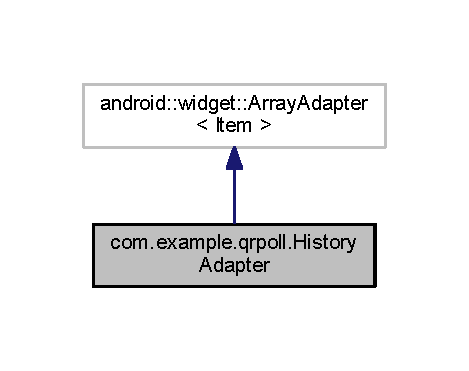
\includegraphics[width=225pt]{classcom_1_1example_1_1qrpoll_1_1_history_adapter__inherit__graph}
\end{center}
\end{figure}


Diagram współpracy dla com.\+example.\+qrpoll.\+History\+Adapter\+:
\nopagebreak
\begin{figure}[H]
\begin{center}
\leavevmode
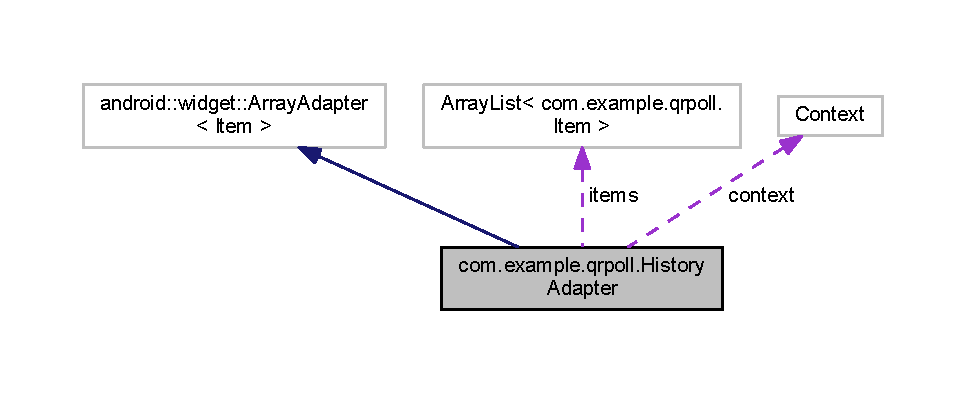
\includegraphics[width=350pt]{classcom_1_1example_1_1qrpoll_1_1_history_adapter__coll__graph}
\end{center}
\end{figure}
\subsection*{Metody publiczne}
\begin{DoxyCompactItemize}
\item 
\hyperlink{classcom_1_1example_1_1qrpoll_1_1_history_adapter_a823c07f9fa09b58051bc1af5ada028b7}{History\+Adapter} (Context \hyperlink{classcom_1_1example_1_1qrpoll_1_1_history_adapter_a118ff9b19fe9e292e2a60fc5b42150f9}{context}, Array\+List$<$ \hyperlink{classcom_1_1example_1_1qrpoll_1_1_item}{Item} $>$ \hyperlink{classcom_1_1example_1_1qrpoll_1_1_history_adapter_adc0f747e0409d63449e90738b935ce1d}{items})
\item 
View \hyperlink{classcom_1_1example_1_1qrpoll_1_1_history_adapter_a272e253c50d2c55359900516f1eab7e6}{get\+View} (int position, View convert\+View, View\+Group parent)
\end{DoxyCompactItemize}
\subsection*{Atrybuty prywatne}
\begin{DoxyCompactItemize}
\item 
final Context \hyperlink{classcom_1_1example_1_1qrpoll_1_1_history_adapter_a118ff9b19fe9e292e2a60fc5b42150f9}{context}
\item 
final Array\+List$<$ \hyperlink{classcom_1_1example_1_1qrpoll_1_1_item}{Item} $>$ \hyperlink{classcom_1_1example_1_1qrpoll_1_1_history_adapter_adc0f747e0409d63449e90738b935ce1d}{items}
\end{DoxyCompactItemize}


\subsection{Opis szczegółowy}
Adapter do wyswietlania historii, \begin{DoxyAuthor}{Autor}
Sliwka layout/row.\+xml 
\end{DoxyAuthor}


Definicja w linii 23 pliku History\+Adapter.\+java.



\subsection{Dokumentacja konstruktora i destruktora}
\hypertarget{classcom_1_1example_1_1qrpoll_1_1_history_adapter_a823c07f9fa09b58051bc1af5ada028b7}{\index{com\+::example\+::qrpoll\+::\+History\+Adapter@{com\+::example\+::qrpoll\+::\+History\+Adapter}!History\+Adapter@{History\+Adapter}}
\index{History\+Adapter@{History\+Adapter}!com\+::example\+::qrpoll\+::\+History\+Adapter@{com\+::example\+::qrpoll\+::\+History\+Adapter}}
\subsubsection[{History\+Adapter}]{\setlength{\rightskip}{0pt plus 5cm}com.\+example.\+qrpoll.\+History\+Adapter.\+History\+Adapter (
\begin{DoxyParamCaption}
\item[{Context}]{context, }
\item[{Array\+List$<$ {\bf Item} $>$}]{items}
\end{DoxyParamCaption}
)}}\label{classcom_1_1example_1_1qrpoll_1_1_history_adapter_a823c07f9fa09b58051bc1af5ada028b7}


Definicja w linii 26 pliku History\+Adapter.\+java.


\begin{DoxyCode}
26                                                                 \{
27         super(\hyperlink{classcom_1_1example_1_1qrpoll_1_1_history_adapter_a118ff9b19fe9e292e2a60fc5b42150f9}{context},R.layout.row,\hyperlink{classcom_1_1example_1_1qrpoll_1_1_history_adapter_adc0f747e0409d63449e90738b935ce1d}{items});
28         this.context=\hyperlink{classcom_1_1example_1_1qrpoll_1_1_history_adapter_a118ff9b19fe9e292e2a60fc5b42150f9}{context};
29         this.items=\hyperlink{classcom_1_1example_1_1qrpoll_1_1_history_adapter_adc0f747e0409d63449e90738b935ce1d}{items};
30     \}
\end{DoxyCode}


\subsection{Dokumentacja funkcji składowych}
\hypertarget{classcom_1_1example_1_1qrpoll_1_1_history_adapter_a272e253c50d2c55359900516f1eab7e6}{\index{com\+::example\+::qrpoll\+::\+History\+Adapter@{com\+::example\+::qrpoll\+::\+History\+Adapter}!get\+View@{get\+View}}
\index{get\+View@{get\+View}!com\+::example\+::qrpoll\+::\+History\+Adapter@{com\+::example\+::qrpoll\+::\+History\+Adapter}}
\subsubsection[{get\+View}]{\setlength{\rightskip}{0pt plus 5cm}View com.\+example.\+qrpoll.\+History\+Adapter.\+get\+View (
\begin{DoxyParamCaption}
\item[{int}]{position, }
\item[{View}]{convert\+View, }
\item[{View\+Group}]{parent}
\end{DoxyParamCaption}
)}}\label{classcom_1_1example_1_1qrpoll_1_1_history_adapter_a272e253c50d2c55359900516f1eab7e6}
wyswietlanie kolejnych rekordow z bazy danych 

Definicja w linii 34 pliku History\+Adapter.\+java.


\begin{DoxyCode}
34                                                                        \{
35         LayoutInflater inflater=(LayoutInflater)\hyperlink{classcom_1_1example_1_1qrpoll_1_1_history_adapter_a118ff9b19fe9e292e2a60fc5b42150f9}{context}.getSystemService(Context.
      LAYOUT\_INFLATER\_SERVICE);
36         View rowView = inflater.inflate(R.layout.row,parent,\textcolor{keyword}{false});
37         TextView labelview=(TextView)rowView.findViewById(R.id.label);
38         TextView valueview=(TextView)rowView.findViewById(R.id.value);
39         TextView dateview=(TextView)rowView.findViewById(R.id.date);
40         TextView roomView=(TextView)rowView.findViewById(R.id.room);
41         labelview.setText(items.get(position).getName());
42         valueview.setText(items.get(position).getValue());
43         dateview.setText(items.get(position).getDate());
44         roomView.setText(items.get(position).getRoom());
45         labelview.setTextColor(Color.BLACK);
46         valueview.setTextColor(Color.BLACK);
47         dateview.setTextColor(Color.BLACK);
48         roomView.setTextColor(Color.BLACK);
49 
50         labelview.setBackgroundColor(Color.rgb(170,170,170));
51         valueview.setBackgroundColor(Color.rgb(175,175,175));
52         dateview.setBackgroundColor(Color.rgb(180,180,180));
53         roomView.setBackgroundColor(Color.rgb(187,187,187));
54         \textcolor{keywordflow}{return} rowView;
55         
56     \}
\end{DoxyCode}


\subsection{Dokumentacja atrybutów składowych}
\hypertarget{classcom_1_1example_1_1qrpoll_1_1_history_adapter_a118ff9b19fe9e292e2a60fc5b42150f9}{\index{com\+::example\+::qrpoll\+::\+History\+Adapter@{com\+::example\+::qrpoll\+::\+History\+Adapter}!context@{context}}
\index{context@{context}!com\+::example\+::qrpoll\+::\+History\+Adapter@{com\+::example\+::qrpoll\+::\+History\+Adapter}}
\subsubsection[{context}]{\setlength{\rightskip}{0pt plus 5cm}final Context com.\+example.\+qrpoll.\+History\+Adapter.\+context\hspace{0.3cm}{\ttfamily [private]}}}\label{classcom_1_1example_1_1qrpoll_1_1_history_adapter_a118ff9b19fe9e292e2a60fc5b42150f9}


Definicja w linii 24 pliku History\+Adapter.\+java.

\hypertarget{classcom_1_1example_1_1qrpoll_1_1_history_adapter_adc0f747e0409d63449e90738b935ce1d}{\index{com\+::example\+::qrpoll\+::\+History\+Adapter@{com\+::example\+::qrpoll\+::\+History\+Adapter}!items@{items}}
\index{items@{items}!com\+::example\+::qrpoll\+::\+History\+Adapter@{com\+::example\+::qrpoll\+::\+History\+Adapter}}
\subsubsection[{items}]{\setlength{\rightskip}{0pt plus 5cm}final Array\+List$<${\bf Item}$>$ com.\+example.\+qrpoll.\+History\+Adapter.\+items\hspace{0.3cm}{\ttfamily [private]}}}\label{classcom_1_1example_1_1qrpoll_1_1_history_adapter_adc0f747e0409d63449e90738b935ce1d}


Definicja w linii 25 pliku History\+Adapter.\+java.



Dokumentacja dla tej klasy została wygenerowana z pliku\+:\begin{DoxyCompactItemize}
\item 
\hyperlink{_history_adapter_8java}{History\+Adapter.\+java}\end{DoxyCompactItemize}

\hypertarget{classcom_1_1example_1_1qrpoll_1_1_history_layout}{\section{Dokumentacja klasy com.\+example.\+qrpoll.\+History\+Layout}
\label{classcom_1_1example_1_1qrpoll_1_1_history_layout}\index{com.\+example.\+qrpoll.\+History\+Layout@{com.\+example.\+qrpoll.\+History\+Layout}}
}


Diagram dziedziczenia dla com.\+example.\+qrpoll.\+History\+Layout\nopagebreak
\begin{figure}[H]
\begin{center}
\leavevmode
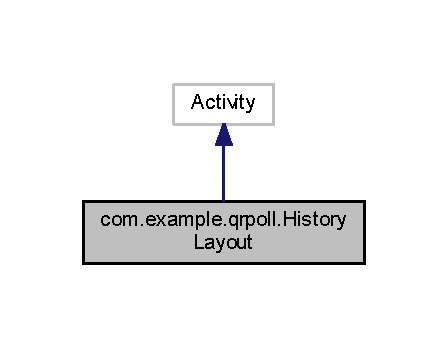
\includegraphics[width=215pt]{classcom_1_1example_1_1qrpoll_1_1_history_layout__inherit__graph}
\end{center}
\end{figure}


Diagram współpracy dla com.\+example.\+qrpoll.\+History\+Layout\+:\nopagebreak
\begin{figure}[H]
\begin{center}
\leavevmode
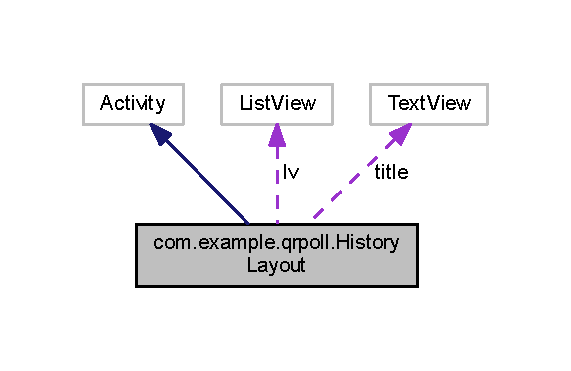
\includegraphics[width=274pt]{classcom_1_1example_1_1qrpoll_1_1_history_layout__coll__graph}
\end{center}
\end{figure}
\subsection*{Metody chronione}
\begin{DoxyCompactItemize}
\item 
void \hyperlink{classcom_1_1example_1_1qrpoll_1_1_history_layout_a693cf48cd1e688ab4bacfd5ce04f26c4}{on\+Create} (Bundle saved\+Instance\+State)
\end{DoxyCompactItemize}
\subsection*{Atrybuty prywatne}
\begin{DoxyCompactItemize}
\item 
List\+View \hyperlink{classcom_1_1example_1_1qrpoll_1_1_history_layout_a12bfa0960dd543b087dd53fb94854a33}{lv}
\item 
Text\+View \hyperlink{classcom_1_1example_1_1qrpoll_1_1_history_layout_afd92cf853727afa975b8763614983bbd}{title}
\end{DoxyCompactItemize}


\subsection{Opis szczegółowy}
Pelnoekranowe activity sluzace do wyswietlania danych z bazy na liscie 

Definicja w linii 38 pliku History\+Layout.\+java.



\subsection{Dokumentacja funkcji składowych}
\hypertarget{classcom_1_1example_1_1qrpoll_1_1_history_layout_a693cf48cd1e688ab4bacfd5ce04f26c4}{\index{com\+::example\+::qrpoll\+::\+History\+Layout@{com\+::example\+::qrpoll\+::\+History\+Layout}!on\+Create@{on\+Create}}
\index{on\+Create@{on\+Create}!com\+::example\+::qrpoll\+::\+History\+Layout@{com\+::example\+::qrpoll\+::\+History\+Layout}}
\subsubsection[{on\+Create}]{\setlength{\rightskip}{0pt plus 5cm}void com.\+example.\+qrpoll.\+History\+Layout.\+on\+Create (
\begin{DoxyParamCaption}
\item[{Bundle}]{saved\+Instance\+State}
\end{DoxyParamCaption}
)\hspace{0.3cm}{\ttfamily [protected]}}}\label{classcom_1_1example_1_1qrpoll_1_1_history_layout_a693cf48cd1e688ab4bacfd5ce04f26c4}
tworzenie widoku,ustawienie adaptera do listy 

Definicja w linii 45 pliku History\+Layout.\+java.


\begin{DoxyCode}
45                                                        \{
46         super.onCreate(savedInstanceState);
47         requestWindowFeature(Window.FEATURE\_CUSTOM\_TITLE);
48         getWindow().setFlags(WindowManager.LayoutParams.FLAG\_FULLSCREEN,
49                 WindowManager.LayoutParams.FLAG\_FULLSCREEN);
50         setContentView(R.layout.activity\_history\_layout);
51         getWindow().setFeatureInt(Window.FEATURE\_CUSTOM\_TITLE, R.layout.window\_title);
52         \hyperlink{classcom_1_1example_1_1qrpoll_1_1_history_layout_afd92cf853727afa975b8763614983bbd}{title}=(TextView)findViewById(R.id.title);
53         title.setText(\textcolor{stringliteral}{"Meetings History"});
54         \hyperlink{classcom_1_1example_1_1qrpoll_1_1_history_layout_a12bfa0960dd543b087dd53fb94854a33}{lv}=(ListView)findViewById(R.id.listView1);
55         lv.setBackgroundColor(Color.parseColor(\textcolor{stringliteral}{"#334455"}));
56         SqlHandler sql=\textcolor{keyword}{new} SqlHandler(getApplication());
57         sql.open();
58         ArrayList<Item>list=sql.getAll();
59         HistoryAdapter adapter=\textcolor{keyword}{new} HistoryAdapter(\textcolor{keyword}{this},list);
60         
61         lv.setAdapter(adapter);
62     \}
\end{DoxyCode}


\subsection{Dokumentacja atrybutów składowych}
\hypertarget{classcom_1_1example_1_1qrpoll_1_1_history_layout_a12bfa0960dd543b087dd53fb94854a33}{\index{com\+::example\+::qrpoll\+::\+History\+Layout@{com\+::example\+::qrpoll\+::\+History\+Layout}!lv@{lv}}
\index{lv@{lv}!com\+::example\+::qrpoll\+::\+History\+Layout@{com\+::example\+::qrpoll\+::\+History\+Layout}}
\subsubsection[{lv}]{\setlength{\rightskip}{0pt plus 5cm}List\+View com.\+example.\+qrpoll.\+History\+Layout.\+lv\hspace{0.3cm}{\ttfamily [private]}}}\label{classcom_1_1example_1_1qrpoll_1_1_history_layout_a12bfa0960dd543b087dd53fb94854a33}


Definicja w linii 39 pliku History\+Layout.\+java.

\hypertarget{classcom_1_1example_1_1qrpoll_1_1_history_layout_afd92cf853727afa975b8763614983bbd}{\index{com\+::example\+::qrpoll\+::\+History\+Layout@{com\+::example\+::qrpoll\+::\+History\+Layout}!title@{title}}
\index{title@{title}!com\+::example\+::qrpoll\+::\+History\+Layout@{com\+::example\+::qrpoll\+::\+History\+Layout}}
\subsubsection[{title}]{\setlength{\rightskip}{0pt plus 5cm}Text\+View com.\+example.\+qrpoll.\+History\+Layout.\+title\hspace{0.3cm}{\ttfamily [private]}}}\label{classcom_1_1example_1_1qrpoll_1_1_history_layout_afd92cf853727afa975b8763614983bbd}


Definicja w linii 40 pliku History\+Layout.\+java.



Dokumentacja dla tej klasy została wygenerowana z pliku\+:\begin{DoxyCompactItemize}
\item 
C\+:/\+Users/\+Wodzu/\+Documents/\+Git\+Hub/\+Projekt\+Zespolowy/\+Android Final + dokumentacja/android/qrpoll/src/com/example/qrpoll/\hyperlink{_history_layout_8java}{History\+Layout.\+java}\end{DoxyCompactItemize}

\hypertarget{classcom_1_1example_1_1qrpoll_1_1_item}{\section{Dokumentacja klasy com.\+example.\+qrpoll.\+Item}
\label{classcom_1_1example_1_1qrpoll_1_1_item}\index{com.\+example.\+qrpoll.\+Item@{com.\+example.\+qrpoll.\+Item}}
}
\subsection*{Metody publiczne}
\begin{DoxyCompactItemize}
\item 
\hyperlink{classcom_1_1example_1_1qrpoll_1_1_item_aa6d7270dec34174ec5a97a8e078a7b73}{Item} (String \hyperlink{classcom_1_1example_1_1qrpoll_1_1_item_a70600dc1190682886f0976b418f13a76}{name}, String \hyperlink{classcom_1_1example_1_1qrpoll_1_1_item_abc0a6b74f1923ca042b9b9d3b48f014c}{value}, String \hyperlink{classcom_1_1example_1_1qrpoll_1_1_item_a47b12c3c00c7a7a9deddb47f139af3cc}{date}, String \hyperlink{classcom_1_1example_1_1qrpoll_1_1_item_ad54518f2889a23bb19316b92711a655c}{room})
\item 
String \hyperlink{classcom_1_1example_1_1qrpoll_1_1_item_aeb31d724eaef2d0ceb0b9869febc6d90}{get\+Name} ()
\item 
String \hyperlink{classcom_1_1example_1_1qrpoll_1_1_item_a278aaa91e51246a75710ecbf25c4ea40}{get\+Value} ()
\item 
String \hyperlink{classcom_1_1example_1_1qrpoll_1_1_item_a184b73561804e998971d7fea88a1d7e0}{get\+Room} ()
\item 
String \hyperlink{classcom_1_1example_1_1qrpoll_1_1_item_a3019ed300c8ffeb23ec841c7fab213c7}{get\+Date} ()
\end{DoxyCompactItemize}
\subsection*{Atrybuty prywatne}
\begin{DoxyCompactItemize}
\item 
String \hyperlink{classcom_1_1example_1_1qrpoll_1_1_item_a70600dc1190682886f0976b418f13a76}{name}
\item 
String \hyperlink{classcom_1_1example_1_1qrpoll_1_1_item_abc0a6b74f1923ca042b9b9d3b48f014c}{value}
\item 
String \hyperlink{classcom_1_1example_1_1qrpoll_1_1_item_a47b12c3c00c7a7a9deddb47f139af3cc}{date}
\item 
String \hyperlink{classcom_1_1example_1_1qrpoll_1_1_item_ad54518f2889a23bb19316b92711a655c}{room}
\end{DoxyCompactItemize}


\subsection{Opis szczegółowy}
Klasa reprezentujaca obiekt, ktory bedzie zapisywany w bazie sql, posiadajacy 4 pola\+: temat, hash,data i pokoj \begin{DoxyAuthor}{Autor}
Sliwka 
\end{DoxyAuthor}


Definicja w linii 17 pliku Item.\+java.



\subsection{Dokumentacja konstruktora i destruktora}
\hypertarget{classcom_1_1example_1_1qrpoll_1_1_item_aa6d7270dec34174ec5a97a8e078a7b73}{\index{com\+::example\+::qrpoll\+::\+Item@{com\+::example\+::qrpoll\+::\+Item}!Item@{Item}}
\index{Item@{Item}!com\+::example\+::qrpoll\+::\+Item@{com\+::example\+::qrpoll\+::\+Item}}
\subsubsection[{Item}]{\setlength{\rightskip}{0pt plus 5cm}com.\+example.\+qrpoll.\+Item.\+Item (
\begin{DoxyParamCaption}
\item[{String}]{name, }
\item[{String}]{value, }
\item[{String}]{date, }
\item[{String}]{room}
\end{DoxyParamCaption}
)}}\label{classcom_1_1example_1_1qrpoll_1_1_item_aa6d7270dec34174ec5a97a8e078a7b73}
konstruktor, ustawia wszyskie wartosci wszystkich pol na podane przez aplikacje 
\begin{DoxyParams}{Parametry}
{\em temat} & spotkania \\
\hline
{\em hash} & spotkania \\
\hline
{\em data} & spotkania \\
\hline
{\em pomieszczenie,gdzie} & odbywa sie spotkanie \\
\hline
\end{DoxyParams}


Definicja w linii 29 pliku Item.\+java.


\begin{DoxyCode}
29                                                                  \{
30         this.name=\hyperlink{classcom_1_1example_1_1qrpoll_1_1_item_a70600dc1190682886f0976b418f13a76}{name};
31         this.value=\hyperlink{classcom_1_1example_1_1qrpoll_1_1_item_abc0a6b74f1923ca042b9b9d3b48f014c}{value};
32         this.date=\hyperlink{classcom_1_1example_1_1qrpoll_1_1_item_a47b12c3c00c7a7a9deddb47f139af3cc}{date};
33         this.room=\hyperlink{classcom_1_1example_1_1qrpoll_1_1_item_ad54518f2889a23bb19316b92711a655c}{room};
34     \}
\end{DoxyCode}


\subsection{Dokumentacja funkcji składowych}
\hypertarget{classcom_1_1example_1_1qrpoll_1_1_item_a3019ed300c8ffeb23ec841c7fab213c7}{\index{com\+::example\+::qrpoll\+::\+Item@{com\+::example\+::qrpoll\+::\+Item}!get\+Date@{get\+Date}}
\index{get\+Date@{get\+Date}!com\+::example\+::qrpoll\+::\+Item@{com\+::example\+::qrpoll\+::\+Item}}
\subsubsection[{get\+Date}]{\setlength{\rightskip}{0pt plus 5cm}String com.\+example.\+qrpoll.\+Item.\+get\+Date (
\begin{DoxyParamCaption}
{}
\end{DoxyParamCaption}
)}}\label{classcom_1_1example_1_1qrpoll_1_1_item_a3019ed300c8ffeb23ec841c7fab213c7}
dostep do zmiennych prywatnych \begin{DoxyReturn}{Zwraca}
data spotkania 
\end{DoxyReturn}


Definicja w linii 60 pliku Item.\+java.


\begin{DoxyCode}
60                            \{
61         \textcolor{keywordflow}{return} \hyperlink{classcom_1_1example_1_1qrpoll_1_1_item_a47b12c3c00c7a7a9deddb47f139af3cc}{date};
62     \}
\end{DoxyCode}
\hypertarget{classcom_1_1example_1_1qrpoll_1_1_item_aeb31d724eaef2d0ceb0b9869febc6d90}{\index{com\+::example\+::qrpoll\+::\+Item@{com\+::example\+::qrpoll\+::\+Item}!get\+Name@{get\+Name}}
\index{get\+Name@{get\+Name}!com\+::example\+::qrpoll\+::\+Item@{com\+::example\+::qrpoll\+::\+Item}}
\subsubsection[{get\+Name}]{\setlength{\rightskip}{0pt plus 5cm}String com.\+example.\+qrpoll.\+Item.\+get\+Name (
\begin{DoxyParamCaption}
{}
\end{DoxyParamCaption}
)}}\label{classcom_1_1example_1_1qrpoll_1_1_item_aeb31d724eaef2d0ceb0b9869febc6d90}
dostep do zmiennych prywatnych \begin{DoxyReturn}{Zwraca}
nazwa spotkania 
\end{DoxyReturn}


Definicja w linii 39 pliku Item.\+java.


\begin{DoxyCode}
39                            \{
40         \textcolor{keywordflow}{return} \hyperlink{classcom_1_1example_1_1qrpoll_1_1_item_a70600dc1190682886f0976b418f13a76}{name};
41     \}
\end{DoxyCode}
\hypertarget{classcom_1_1example_1_1qrpoll_1_1_item_a184b73561804e998971d7fea88a1d7e0}{\index{com\+::example\+::qrpoll\+::\+Item@{com\+::example\+::qrpoll\+::\+Item}!get\+Room@{get\+Room}}
\index{get\+Room@{get\+Room}!com\+::example\+::qrpoll\+::\+Item@{com\+::example\+::qrpoll\+::\+Item}}
\subsubsection[{get\+Room}]{\setlength{\rightskip}{0pt plus 5cm}String com.\+example.\+qrpoll.\+Item.\+get\+Room (
\begin{DoxyParamCaption}
{}
\end{DoxyParamCaption}
)}}\label{classcom_1_1example_1_1qrpoll_1_1_item_a184b73561804e998971d7fea88a1d7e0}
dostep do zmiennych prywatnych \begin{DoxyReturn}{Zwraca}
adres gdzie odbywa sie spotkanie 
\end{DoxyReturn}


Definicja w linii 53 pliku Item.\+java.


\begin{DoxyCode}
53                            \{
54         \textcolor{keywordflow}{return} \hyperlink{classcom_1_1example_1_1qrpoll_1_1_item_ad54518f2889a23bb19316b92711a655c}{room};
55     \}
\end{DoxyCode}
\hypertarget{classcom_1_1example_1_1qrpoll_1_1_item_a278aaa91e51246a75710ecbf25c4ea40}{\index{com\+::example\+::qrpoll\+::\+Item@{com\+::example\+::qrpoll\+::\+Item}!get\+Value@{get\+Value}}
\index{get\+Value@{get\+Value}!com\+::example\+::qrpoll\+::\+Item@{com\+::example\+::qrpoll\+::\+Item}}
\subsubsection[{get\+Value}]{\setlength{\rightskip}{0pt plus 5cm}String com.\+example.\+qrpoll.\+Item.\+get\+Value (
\begin{DoxyParamCaption}
{}
\end{DoxyParamCaption}
)}}\label{classcom_1_1example_1_1qrpoll_1_1_item_a278aaa91e51246a75710ecbf25c4ea40}
dostep do zmiennych prywatnych \begin{DoxyReturn}{Zwraca}
hash spotkania 
\end{DoxyReturn}


Definicja w linii 46 pliku Item.\+java.


\begin{DoxyCode}
46                             \{
47         \textcolor{keywordflow}{return} \hyperlink{classcom_1_1example_1_1qrpoll_1_1_item_abc0a6b74f1923ca042b9b9d3b48f014c}{value};
48     \}
\end{DoxyCode}


\subsection{Dokumentacja atrybutów składowych}
\hypertarget{classcom_1_1example_1_1qrpoll_1_1_item_a47b12c3c00c7a7a9deddb47f139af3cc}{\index{com\+::example\+::qrpoll\+::\+Item@{com\+::example\+::qrpoll\+::\+Item}!date@{date}}
\index{date@{date}!com\+::example\+::qrpoll\+::\+Item@{com\+::example\+::qrpoll\+::\+Item}}
\subsubsection[{date}]{\setlength{\rightskip}{0pt plus 5cm}String com.\+example.\+qrpoll.\+Item.\+date\hspace{0.3cm}{\ttfamily [private]}}}\label{classcom_1_1example_1_1qrpoll_1_1_item_a47b12c3c00c7a7a9deddb47f139af3cc}


Definicja w linii 20 pliku Item.\+java.

\hypertarget{classcom_1_1example_1_1qrpoll_1_1_item_a70600dc1190682886f0976b418f13a76}{\index{com\+::example\+::qrpoll\+::\+Item@{com\+::example\+::qrpoll\+::\+Item}!name@{name}}
\index{name@{name}!com\+::example\+::qrpoll\+::\+Item@{com\+::example\+::qrpoll\+::\+Item}}
\subsubsection[{name}]{\setlength{\rightskip}{0pt plus 5cm}String com.\+example.\+qrpoll.\+Item.\+name\hspace{0.3cm}{\ttfamily [private]}}}\label{classcom_1_1example_1_1qrpoll_1_1_item_a70600dc1190682886f0976b418f13a76}


Definicja w linii 18 pliku Item.\+java.

\hypertarget{classcom_1_1example_1_1qrpoll_1_1_item_ad54518f2889a23bb19316b92711a655c}{\index{com\+::example\+::qrpoll\+::\+Item@{com\+::example\+::qrpoll\+::\+Item}!room@{room}}
\index{room@{room}!com\+::example\+::qrpoll\+::\+Item@{com\+::example\+::qrpoll\+::\+Item}}
\subsubsection[{room}]{\setlength{\rightskip}{0pt plus 5cm}String com.\+example.\+qrpoll.\+Item.\+room\hspace{0.3cm}{\ttfamily [private]}}}\label{classcom_1_1example_1_1qrpoll_1_1_item_ad54518f2889a23bb19316b92711a655c}


Definicja w linii 21 pliku Item.\+java.

\hypertarget{classcom_1_1example_1_1qrpoll_1_1_item_abc0a6b74f1923ca042b9b9d3b48f014c}{\index{com\+::example\+::qrpoll\+::\+Item@{com\+::example\+::qrpoll\+::\+Item}!value@{value}}
\index{value@{value}!com\+::example\+::qrpoll\+::\+Item@{com\+::example\+::qrpoll\+::\+Item}}
\subsubsection[{value}]{\setlength{\rightskip}{0pt plus 5cm}String com.\+example.\+qrpoll.\+Item.\+value\hspace{0.3cm}{\ttfamily [private]}}}\label{classcom_1_1example_1_1qrpoll_1_1_item_abc0a6b74f1923ca042b9b9d3b48f014c}


Definicja w linii 19 pliku Item.\+java.



Dokumentacja dla tej klasy została wygenerowana z pliku\+:\begin{DoxyCompactItemize}
\item 
C\+:/\+Users/\+Wodzu/\+Documents/\+Git\+Hub/\+Projekt\+Zespolowy/\+Android Final + dokumentacja/android/qrpoll/src/com/example/qrpoll/\hyperlink{_item_8java}{Item.\+java}\end{DoxyCompactItemize}

\hypertarget{classcom_1_1example_1_1qrpoll_1_1_main_activity}{\section{Dokumentacja klasy com.\+example.\+qrpoll.\+Main\+Activity}
\label{classcom_1_1example_1_1qrpoll_1_1_main_activity}\index{com.\+example.\+qrpoll.\+Main\+Activity@{com.\+example.\+qrpoll.\+Main\+Activity}}
}


Diagram dziedziczenia dla com.\+example.\+qrpoll.\+Main\+Activity
\nopagebreak
\begin{figure}[H]
\begin{center}
\leavevmode
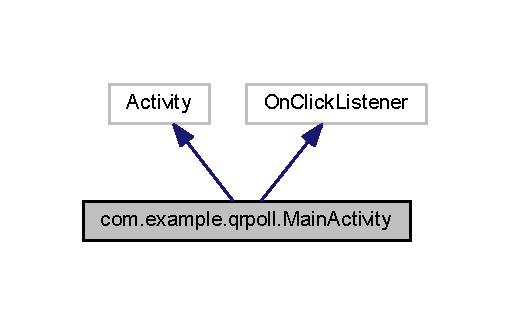
\includegraphics[width=245pt]{classcom_1_1example_1_1qrpoll_1_1_main_activity__inherit__graph}
\end{center}
\end{figure}


Diagram współpracy dla com.\+example.\+qrpoll.\+Main\+Activity\+:
\nopagebreak
\begin{figure}[H]
\begin{center}
\leavevmode
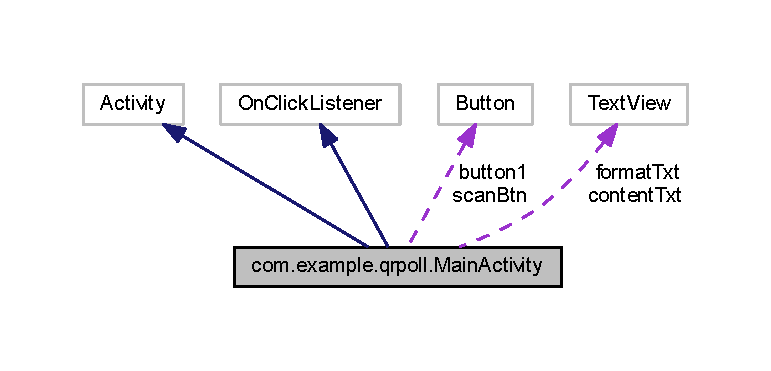
\includegraphics[width=350pt]{classcom_1_1example_1_1qrpoll_1_1_main_activity__coll__graph}
\end{center}
\end{figure}
\subsection*{Komponenty}
\begin{DoxyCompactItemize}
\item 
class \hyperlink{classcom_1_1example_1_1qrpoll_1_1_main_activity_1_1_placeholder_fragment}{Placeholder\+Fragment}
\end{DoxyCompactItemize}
\subsection*{Metody publiczne}
\begin{DoxyCompactItemize}
\item 
void \hyperlink{classcom_1_1example_1_1qrpoll_1_1_main_activity_a400e30efc907d9726298482730d4243d}{on\+Click} (View v)
\item 
void \hyperlink{classcom_1_1example_1_1qrpoll_1_1_main_activity_ab7dc0b400a4156ce07ec51712c638b5b}{on\+Activity\+Result} (int request\+Code, int result\+Code, Intent intent)
\item 
void \hyperlink{classcom_1_1example_1_1qrpoll_1_1_main_activity_ac108fe2528d7657f970d61d49639e6ac}{to\+Poll\+Activity} (String scan\+Result)
\item 
boolean \hyperlink{classcom_1_1example_1_1qrpoll_1_1_main_activity_a0433b5df97dcca7db8593f32d8d033b9}{check\+Wifi} ()
\item 
boolean \hyperlink{classcom_1_1example_1_1qrpoll_1_1_main_activity_af92255e3a196405eeb55e06bb625d435}{check\+Network} ()
\item 
boolean \hyperlink{classcom_1_1example_1_1qrpoll_1_1_main_activity_adbf1a4ac0f7940113677f58a1d85f295}{on\+Create\+Options\+Menu} (Menu menu)
\item 
boolean \hyperlink{classcom_1_1example_1_1qrpoll_1_1_main_activity_acb1d82fc0d1505cc54762cb028826c3c}{on\+Options\+Item\+Selected} (Menu\+Item item)
\end{DoxyCompactItemize}
\subsection*{Metody chronione}
\begin{DoxyCompactItemize}
\item 
void \hyperlink{classcom_1_1example_1_1qrpoll_1_1_main_activity_a6870a3a43acb7f6024f45467a0a786fd}{on\+Create} (Bundle saved\+Instance\+State)
\end{DoxyCompactItemize}
\subsection*{Atrybuty pakietu}
\begin{DoxyCompactItemize}
\item 
Text\+View \hyperlink{classcom_1_1example_1_1qrpoll_1_1_main_activity_aee6c7adea75224ec647353db3ca58124}{content\+Txt}
\end{DoxyCompactItemize}
\subsection*{Atrybuty prywatne}
\begin{DoxyCompactItemize}
\item 
Button \hyperlink{classcom_1_1example_1_1qrpoll_1_1_main_activity_a24aa61710d9b421c0d23ab545b4f8b99}{scan\+Btn}
\item 
Button \hyperlink{classcom_1_1example_1_1qrpoll_1_1_main_activity_a3c62b040921525ab5c9944e97e08f639}{button1}
\item 
Text\+View \hyperlink{classcom_1_1example_1_1qrpoll_1_1_main_activity_ac2f96df8bbad653bdd8630d749a23ddc}{format\+Txt}
\end{DoxyCompactItemize}


\subsection{Opis szczegółowy}
Activity, ktore laduje sie przy starcie aplikacji, umozliwia przejscie do skanowania oraz wyswietlenie historii \begin{DoxyAuthor}{Autor}
Sliwka,Piotrek 
\end{DoxyAuthor}


Definicja w linii 31 pliku Main\+Activity.\+java.



\subsection{Dokumentacja funkcji składowych}
\hypertarget{classcom_1_1example_1_1qrpoll_1_1_main_activity_af92255e3a196405eeb55e06bb625d435}{\index{com\+::example\+::qrpoll\+::\+Main\+Activity@{com\+::example\+::qrpoll\+::\+Main\+Activity}!check\+Network@{check\+Network}}
\index{check\+Network@{check\+Network}!com\+::example\+::qrpoll\+::\+Main\+Activity@{com\+::example\+::qrpoll\+::\+Main\+Activity}}
\subsubsection[{check\+Network}]{\setlength{\rightskip}{0pt plus 5cm}boolean com.\+example.\+qrpoll.\+Main\+Activity.\+check\+Network (
\begin{DoxyParamCaption}
{}
\end{DoxyParamCaption}
)}}\label{classcom_1_1example_1_1qrpoll_1_1_main_activity_af92255e3a196405eeb55e06bb625d435}
sprawdzenie danych pakietowych \begin{DoxyReturn}{Zwraca}

\end{DoxyReturn}


Definicja w linii 159 pliku Main\+Activity.\+java.


\begin{DoxyCode}
159                                  \{
160         ConnectivityManager cm=(ConnectivityManager)getSystemService(Context.CONNECTIVITY\_SERVICE);
161         NetworkInfo ni=cm.getNetworkInfo(ConnectivityManager.TYPE\_MOBILE);
162         \textcolor{keywordflow}{return} ni.isConnected();
163     \}
\end{DoxyCode}
\hypertarget{classcom_1_1example_1_1qrpoll_1_1_main_activity_a0433b5df97dcca7db8593f32d8d033b9}{\index{com\+::example\+::qrpoll\+::\+Main\+Activity@{com\+::example\+::qrpoll\+::\+Main\+Activity}!check\+Wifi@{check\+Wifi}}
\index{check\+Wifi@{check\+Wifi}!com\+::example\+::qrpoll\+::\+Main\+Activity@{com\+::example\+::qrpoll\+::\+Main\+Activity}}
\subsubsection[{check\+Wifi}]{\setlength{\rightskip}{0pt plus 5cm}boolean com.\+example.\+qrpoll.\+Main\+Activity.\+check\+Wifi (
\begin{DoxyParamCaption}
{}
\end{DoxyParamCaption}
)}}\label{classcom_1_1example_1_1qrpoll_1_1_main_activity_a0433b5df97dcca7db8593f32d8d033b9}
sprawdzenie stanu wifi \begin{DoxyReturn}{Zwraca}

\end{DoxyReturn}


Definicja w linii 151 pliku Main\+Activity.\+java.


\begin{DoxyCode}
151                               \{
152         WifiManager wifi=(WifiManager)getSystemService(Context.WIFI\_SERVICE);
153         \textcolor{keywordflow}{return} wifi.isWifiEnabled();
154     \}
\end{DoxyCode}
\hypertarget{classcom_1_1example_1_1qrpoll_1_1_main_activity_ab7dc0b400a4156ce07ec51712c638b5b}{\index{com\+::example\+::qrpoll\+::\+Main\+Activity@{com\+::example\+::qrpoll\+::\+Main\+Activity}!on\+Activity\+Result@{on\+Activity\+Result}}
\index{on\+Activity\+Result@{on\+Activity\+Result}!com\+::example\+::qrpoll\+::\+Main\+Activity@{com\+::example\+::qrpoll\+::\+Main\+Activity}}
\subsubsection[{on\+Activity\+Result}]{\setlength{\rightskip}{0pt plus 5cm}void com.\+example.\+qrpoll.\+Main\+Activity.\+on\+Activity\+Result (
\begin{DoxyParamCaption}
\item[{int}]{request\+Code, }
\item[{int}]{result\+Code, }
\item[{Intent}]{intent}
\end{DoxyParamCaption}
)}}\label{classcom_1_1example_1_1qrpoll_1_1_main_activity_ab7dc0b400a4156ce07ec51712c638b5b}
metoda przetwarzajaca wynik skanowania 

Definicja w linii 87 pliku Main\+Activity.\+java.


\begin{DoxyCode}
87                                                                                  \{
88         \textcolor{keywordflow}{try}\{
89         \textcolor{keywordflow}{if}(requestCode == IntentIntegrator.REQUEST\_CODE)\{
90             \textcolor{comment}{//retrieve scan result}
91             IntentResult scanningResult = IntentIntegrator.parseActivityResult(requestCode, resultCode, 
      intent);
92             
93             \textcolor{keywordflow}{if} (scanningResult != null) \{
94                 \textcolor{comment}{//we have a result}
95                 String scanContent = scanningResult.getContents();
96                 \hyperlink{classcom_1_1example_1_1qrpoll_1_1_main_activity_ac108fe2528d7657f970d61d49639e6ac}{toPollActivity}(scanContent);
97                 
98                 
99             \}
100             \textcolor{keywordflow}{else}\{
101                 Toast toast = Toast.makeText(getApplicationContext(),
102                     \textcolor{stringliteral}{"No scan data received!"}, Toast.LENGTH\_SHORT);
103                 toast.show();
104             \}
105             
106             
107                         
108         \}
109         \}\textcolor{keywordflow}{catch}(NullPointerException e)\{
110             Toast toast = Toast.makeText(getApplicationContext(),
111                     \textcolor{stringliteral}{"Przerwano skanowanie"}, Toast.LENGTH\_SHORT);
112                 toast.show();
113         \}
114     \}
\end{DoxyCode}
\hypertarget{classcom_1_1example_1_1qrpoll_1_1_main_activity_a400e30efc907d9726298482730d4243d}{\index{com\+::example\+::qrpoll\+::\+Main\+Activity@{com\+::example\+::qrpoll\+::\+Main\+Activity}!on\+Click@{on\+Click}}
\index{on\+Click@{on\+Click}!com\+::example\+::qrpoll\+::\+Main\+Activity@{com\+::example\+::qrpoll\+::\+Main\+Activity}}
\subsubsection[{on\+Click}]{\setlength{\rightskip}{0pt plus 5cm}void com.\+example.\+qrpoll.\+Main\+Activity.\+on\+Click (
\begin{DoxyParamCaption}
\item[{View}]{v}
\end{DoxyParamCaption}
)}}\label{classcom_1_1example_1_1qrpoll_1_1_main_activity_a400e30efc907d9726298482730d4243d}
przypisanie akcji do przycisku skanowania 

Definicja w linii 76 pliku Main\+Activity.\+java.


\begin{DoxyCode}
76                                 \{
77         \textcolor{keywordflow}{if}(v.getId()==R.id.scan\_button)\{
78             \textcolor{comment}{//scan}
79             IntentIntegrator scanIntegrator = \textcolor{keyword}{new} IntentIntegrator(\textcolor{keyword}{this});
80             scanIntegrator.initiateScan();
81         \}
82         
83     \}
\end{DoxyCode}
\hypertarget{classcom_1_1example_1_1qrpoll_1_1_main_activity_a6870a3a43acb7f6024f45467a0a786fd}{\index{com\+::example\+::qrpoll\+::\+Main\+Activity@{com\+::example\+::qrpoll\+::\+Main\+Activity}!on\+Create@{on\+Create}}
\index{on\+Create@{on\+Create}!com\+::example\+::qrpoll\+::\+Main\+Activity@{com\+::example\+::qrpoll\+::\+Main\+Activity}}
\subsubsection[{on\+Create}]{\setlength{\rightskip}{0pt plus 5cm}void com.\+example.\+qrpoll.\+Main\+Activity.\+on\+Create (
\begin{DoxyParamCaption}
\item[{Bundle}]{saved\+Instance\+State}
\end{DoxyParamCaption}
)\hspace{0.3cm}{\ttfamily [protected]}}}\label{classcom_1_1example_1_1qrpoll_1_1_main_activity_a6870a3a43acb7f6024f45467a0a786fd}
tworzenie startowego widoku aplikacji 

Definicja w linii 42 pliku Main\+Activity.\+java.


\begin{DoxyCode}
42                                                        \{
43         super.onCreate(savedInstanceState);
44         setContentView(R.layout.activity\_main);
45         
46         \hyperlink{classcom_1_1example_1_1qrpoll_1_1_main_activity_a24aa61710d9b421c0d23ab545b4f8b99}{scanBtn} = (Button)findViewById(R.id.scan\_button);
47         \hyperlink{classcom_1_1example_1_1qrpoll_1_1_main_activity_a3c62b040921525ab5c9944e97e08f639}{button1}=(Button)findViewById(R.id.button1);
48         \hyperlink{classcom_1_1example_1_1qrpoll_1_1_main_activity_ac2f96df8bbad653bdd8630d749a23ddc}{formatTxt} = (TextView)findViewById(R.id.scan\_format);
49         \hyperlink{classcom_1_1example_1_1qrpoll_1_1_main_activity_aee6c7adea75224ec647353db3ca58124}{contentTxt} = (TextView)findViewById(R.id.scan\_content);
50         
51         scanBtn.setOnClickListener(\textcolor{keyword}{this});
52         SqlHandler sql=\textcolor{keyword}{new} SqlHandler(getApplication());
53         sql.open();
54         sql.close();
55         \textcolor{keywordflow}{if}(!\hyperlink{classcom_1_1example_1_1qrpoll_1_1_main_activity_af92255e3a196405eeb55e06bb625d435}{checkNetwork}())\{
56             \textcolor{keywordflow}{if}(!\hyperlink{classcom_1_1example_1_1qrpoll_1_1_main_activity_a0433b5df97dcca7db8593f32d8d033b9}{checkWifi}())\{
57                 AlertDialog.Builder adb=\textcolor{keyword}{new} AlertDialog.Builder(\textcolor{keyword}{this});
58                 adb.setTitle(\textcolor{stringliteral}{"Brak polaczenia"});
59                 adb.setMessage(\textcolor{stringliteral}{"Nacisnij ok aby wlaczyc WIFI"}).setCancelable(\textcolor{keyword}{false}).setNeutralButton(\textcolor{stringliteral}{"OK"}, \textcolor{keyword}{
      new} DialogInterface.OnClickListener() \{
60                     
61                     @Override
62                     \textcolor{keyword}{public} \textcolor{keywordtype}{void} \hyperlink{classcom_1_1example_1_1qrpoll_1_1_main_activity_a400e30efc907d9726298482730d4243d}{onClick}(DialogInterface dialog, \textcolor{keywordtype}{int} which) \{
63                         WifiManager wifi=(WifiManager)getSystemService(Context.WIFI\_SERVICE);
64                         wifi.setWifiEnabled(\textcolor{keyword}{true});
65                     \}
66                 \});
67                 AlertDialog ad=adb.create();
68                 ad.show();
69             \}
70         \}
71     \}
\end{DoxyCode}
\hypertarget{classcom_1_1example_1_1qrpoll_1_1_main_activity_adbf1a4ac0f7940113677f58a1d85f295}{\index{com\+::example\+::qrpoll\+::\+Main\+Activity@{com\+::example\+::qrpoll\+::\+Main\+Activity}!on\+Create\+Options\+Menu@{on\+Create\+Options\+Menu}}
\index{on\+Create\+Options\+Menu@{on\+Create\+Options\+Menu}!com\+::example\+::qrpoll\+::\+Main\+Activity@{com\+::example\+::qrpoll\+::\+Main\+Activity}}
\subsubsection[{on\+Create\+Options\+Menu}]{\setlength{\rightskip}{0pt plus 5cm}boolean com.\+example.\+qrpoll.\+Main\+Activity.\+on\+Create\+Options\+Menu (
\begin{DoxyParamCaption}
\item[{Menu}]{menu}
\end{DoxyParamCaption}
)}}\label{classcom_1_1example_1_1qrpoll_1_1_main_activity_adbf1a4ac0f7940113677f58a1d85f295}
tworzenie menu 

Definicja w linii 169 pliku Main\+Activity.\+java.


\begin{DoxyCode}
169                                                   \{
170         
171         \textcolor{comment}{// Inflate the menu; this adds items to the action bar if it is present.}
172         getMenuInflater().inflate(R.menu.main, menu);
173         \textcolor{keywordflow}{return} \textcolor{keyword}{true};
174     \}
\end{DoxyCode}
\hypertarget{classcom_1_1example_1_1qrpoll_1_1_main_activity_acb1d82fc0d1505cc54762cb028826c3c}{\index{com\+::example\+::qrpoll\+::\+Main\+Activity@{com\+::example\+::qrpoll\+::\+Main\+Activity}!on\+Options\+Item\+Selected@{on\+Options\+Item\+Selected}}
\index{on\+Options\+Item\+Selected@{on\+Options\+Item\+Selected}!com\+::example\+::qrpoll\+::\+Main\+Activity@{com\+::example\+::qrpoll\+::\+Main\+Activity}}
\subsubsection[{on\+Options\+Item\+Selected}]{\setlength{\rightskip}{0pt plus 5cm}boolean com.\+example.\+qrpoll.\+Main\+Activity.\+on\+Options\+Item\+Selected (
\begin{DoxyParamCaption}
\item[{Menu\+Item}]{item}
\end{DoxyParamCaption}
)}}\label{classcom_1_1example_1_1qrpoll_1_1_main_activity_acb1d82fc0d1505cc54762cb028826c3c}
przypisanie akcji do przyciskow menu 

Definicja w linii 180 pliku Main\+Activity.\+java.


\begin{DoxyCode}
180                                                         \{
181         \textcolor{comment}{// Handle action bar item clicks here. The action bar will}
182         \textcolor{comment}{// automatically handle clicks on the Home/Up button, so long}
183         \textcolor{comment}{// as you specify a parent activity in AndroidManifest.xml.}
184         \textcolor{keywordtype}{int} \textcolor{keywordtype}{id} = item.getItemId();
185         \textcolor{comment}{//start historii}
186         \textcolor{keywordflow}{if} (\textcolor{keywordtype}{id} == R.id.action\_settings) \{
187             Intent it=\textcolor{keyword}{new} Intent(getApplication(),HistoryLayout.class);
188             startActivity(it);
189             
190             \textcolor{keywordflow}{return} \textcolor{keyword}{true};
191         \}
192         \textcolor{keywordflow}{return} super.onOptionsItemSelected(item);
193     \}
\end{DoxyCode}
\hypertarget{classcom_1_1example_1_1qrpoll_1_1_main_activity_ac108fe2528d7657f970d61d49639e6ac}{\index{com\+::example\+::qrpoll\+::\+Main\+Activity@{com\+::example\+::qrpoll\+::\+Main\+Activity}!to\+Poll\+Activity@{to\+Poll\+Activity}}
\index{to\+Poll\+Activity@{to\+Poll\+Activity}!com\+::example\+::qrpoll\+::\+Main\+Activity@{com\+::example\+::qrpoll\+::\+Main\+Activity}}
\subsubsection[{to\+Poll\+Activity}]{\setlength{\rightskip}{0pt plus 5cm}void com.\+example.\+qrpoll.\+Main\+Activity.\+to\+Poll\+Activity (
\begin{DoxyParamCaption}
\item[{String}]{scan\+Result}
\end{DoxyParamCaption}
)}}\label{classcom_1_1example_1_1qrpoll_1_1_main_activity_ac108fe2528d7657f970d61d49639e6ac}
startuje nowe activity 
\begin{DoxyParams}{Parametry}
{\em scan\+Result} & zeskanowany adres url \\
\hline
\end{DoxyParams}


Definicja w linii 120 pliku Main\+Activity.\+java.


\begin{DoxyCode}
120                                                  \{
121         \textcolor{keywordflow}{if}(!scanResult.isEmpty())\{
122             Intent intent = \textcolor{keyword}{new} Intent(\textcolor{keyword}{this}, PollActivity.class);
123             intent.putExtra(\textcolor{stringliteral}{"scanResult"}, scanResult);
124             intent.putExtra(\textcolor{stringliteral}{"message"}, \textcolor{stringliteral}{"none"});
125             \textcolor{keywordflow}{if}(\hyperlink{classcom_1_1example_1_1qrpoll_1_1_main_activity_a0433b5df97dcca7db8593f32d8d033b9}{checkWifi}()||\hyperlink{classcom_1_1example_1_1qrpoll_1_1_main_activity_af92255e3a196405eeb55e06bb625d435}{checkNetwork}())\{
126                 \textcolor{keywordflow}{try}\{
127                 startActivity(intent);
128                 finish();
129                 \}\textcolor{keywordflow}{catch}(RuntimeException e)\{
130                     Toast toast = Toast.makeText(getApplicationContext(),
131                             \textcolor{stringliteral}{"Nie znaleziono strony o danym adresie!"}, Toast.LENGTH\_SHORT);
132                         toast.show();
133                 \}
134                 
135             \}\textcolor{keywordflow}{else}\{
136                 Toast toast = Toast.makeText(getApplicationContext(),
137                         \textcolor{stringliteral}{"Brak polaczenia,nie mozna kontynuowac!"}, Toast.LENGTH\_SHORT);
138                     toast.show();
139             \}
140         
141         \}\textcolor{keywordflow}{else}\{
142             Toast toast = Toast.makeText(getApplicationContext(),
143                     \textcolor{stringliteral}{"No scan data received!"}, Toast.LENGTH\_SHORT);
144                 toast.show();
145         \}
146     \}
\end{DoxyCode}


\subsection{Dokumentacja atrybutów składowych}
\hypertarget{classcom_1_1example_1_1qrpoll_1_1_main_activity_a3c62b040921525ab5c9944e97e08f639}{\index{com\+::example\+::qrpoll\+::\+Main\+Activity@{com\+::example\+::qrpoll\+::\+Main\+Activity}!button1@{button1}}
\index{button1@{button1}!com\+::example\+::qrpoll\+::\+Main\+Activity@{com\+::example\+::qrpoll\+::\+Main\+Activity}}
\subsubsection[{button1}]{\setlength{\rightskip}{0pt plus 5cm}Button com.\+example.\+qrpoll.\+Main\+Activity.\+button1\hspace{0.3cm}{\ttfamily [private]}}}\label{classcom_1_1example_1_1qrpoll_1_1_main_activity_a3c62b040921525ab5c9944e97e08f639}


Definicja w linii 35 pliku Main\+Activity.\+java.

\hypertarget{classcom_1_1example_1_1qrpoll_1_1_main_activity_aee6c7adea75224ec647353db3ca58124}{\index{com\+::example\+::qrpoll\+::\+Main\+Activity@{com\+::example\+::qrpoll\+::\+Main\+Activity}!content\+Txt@{content\+Txt}}
\index{content\+Txt@{content\+Txt}!com\+::example\+::qrpoll\+::\+Main\+Activity@{com\+::example\+::qrpoll\+::\+Main\+Activity}}
\subsubsection[{content\+Txt}]{\setlength{\rightskip}{0pt plus 5cm}Text\+View com.\+example.\+qrpoll.\+Main\+Activity.\+content\+Txt\hspace{0.3cm}{\ttfamily [package]}}}\label{classcom_1_1example_1_1qrpoll_1_1_main_activity_aee6c7adea75224ec647353db3ca58124}


Definicja w linii 36 pliku Main\+Activity.\+java.

\hypertarget{classcom_1_1example_1_1qrpoll_1_1_main_activity_ac2f96df8bbad653bdd8630d749a23ddc}{\index{com\+::example\+::qrpoll\+::\+Main\+Activity@{com\+::example\+::qrpoll\+::\+Main\+Activity}!format\+Txt@{format\+Txt}}
\index{format\+Txt@{format\+Txt}!com\+::example\+::qrpoll\+::\+Main\+Activity@{com\+::example\+::qrpoll\+::\+Main\+Activity}}
\subsubsection[{format\+Txt}]{\setlength{\rightskip}{0pt plus 5cm}Text\+View com.\+example.\+qrpoll.\+Main\+Activity.\+format\+Txt\hspace{0.3cm}{\ttfamily [private]}}}\label{classcom_1_1example_1_1qrpoll_1_1_main_activity_ac2f96df8bbad653bdd8630d749a23ddc}


Definicja w linii 36 pliku Main\+Activity.\+java.

\hypertarget{classcom_1_1example_1_1qrpoll_1_1_main_activity_a24aa61710d9b421c0d23ab545b4f8b99}{\index{com\+::example\+::qrpoll\+::\+Main\+Activity@{com\+::example\+::qrpoll\+::\+Main\+Activity}!scan\+Btn@{scan\+Btn}}
\index{scan\+Btn@{scan\+Btn}!com\+::example\+::qrpoll\+::\+Main\+Activity@{com\+::example\+::qrpoll\+::\+Main\+Activity}}
\subsubsection[{scan\+Btn}]{\setlength{\rightskip}{0pt plus 5cm}Button com.\+example.\+qrpoll.\+Main\+Activity.\+scan\+Btn\hspace{0.3cm}{\ttfamily [private]}}}\label{classcom_1_1example_1_1qrpoll_1_1_main_activity_a24aa61710d9b421c0d23ab545b4f8b99}


Definicja w linii 34 pliku Main\+Activity.\+java.



Dokumentacja dla tej klasy została wygenerowana z pliku\+:\begin{DoxyCompactItemize}
\item 
\hyperlink{_main_activity_8java}{Main\+Activity.\+java}\end{DoxyCompactItemize}

\hypertarget{classcom_1_1example_1_1qrpoll_1_1_my_http_u_r_l_connection}{\section{Dokumentacja klasy com.\+example.\+qrpoll.\+My\+Http\+U\+R\+L\+Connection}
\label{classcom_1_1example_1_1qrpoll_1_1_my_http_u_r_l_connection}\index{com.\+example.\+qrpoll.\+My\+Http\+U\+R\+L\+Connection@{com.\+example.\+qrpoll.\+My\+Http\+U\+R\+L\+Connection}}
}
\subsection*{Statyczne metody publiczne}
\begin{DoxyCompactItemize}
\item 
static String \hyperlink{classcom_1_1example_1_1qrpoll_1_1_my_http_u_r_l_connection_a2da0c692c90b6a847356d6573c288acc}{get} (String url)  throws Client\+Protocol\+Exception, I\+O\+Exception, Exception404
\end{DoxyCompactItemize}


\subsection{Opis szczegółowy}
klasa odpowiadajaca za polaczenie sie z serwerem i pobranie zawartosci strony na serwerze strony zwracaja dane przy uzyciu J\+S\+O\+N \begin{DoxyAuthor}{Autor}
Piotrek 
\end{DoxyAuthor}


Definicja w linii 32 pliku My\+Http\+U\+R\+L\+Connection.\+java.



\subsection{Dokumentacja funkcji składowych}
\hypertarget{classcom_1_1example_1_1qrpoll_1_1_my_http_u_r_l_connection_a2da0c692c90b6a847356d6573c288acc}{\index{com\+::example\+::qrpoll\+::\+My\+Http\+U\+R\+L\+Connection@{com\+::example\+::qrpoll\+::\+My\+Http\+U\+R\+L\+Connection}!get@{get}}
\index{get@{get}!com\+::example\+::qrpoll\+::\+My\+Http\+U\+R\+L\+Connection@{com\+::example\+::qrpoll\+::\+My\+Http\+U\+R\+L\+Connection}}
\subsubsection[{get}]{\setlength{\rightskip}{0pt plus 5cm}static String com.\+example.\+qrpoll.\+My\+Http\+U\+R\+L\+Connection.\+get (
\begin{DoxyParamCaption}
\item[{String}]{url}
\end{DoxyParamCaption}
) throws Client\+Protocol\+Exception, I\+O\+Exception, {\bf Exception404}\hspace{0.3cm}{\ttfamily [static]}}}\label{classcom_1_1example_1_1qrpoll_1_1_my_http_u_r_l_connection_a2da0c692c90b6a847356d6573c288acc}
pobieranie zawartosci strony z serwera 
\begin{DoxyParams}{Parametry}
{\em url} & adres url strony z ktora chcemy sie polaczyc \\
\hline
\end{DoxyParams}
\begin{DoxyReturn}{Zwraca}
zawartosc strony 
\end{DoxyReturn}

\begin{DoxyExceptions}{Wyjątki}
{\em Client\+Protocol\+Exception} & \\
\hline
{\em I\+O\+Exception} & \\
\hline
{\em \hyperlink{classcom_1_1example_1_1qrpoll_1_1_exception404}{Exception404}} & \\
\hline
\end{DoxyExceptions}


Definicja w linii 41 pliku My\+Http\+U\+R\+L\+Connection.\+java.


\begin{DoxyCode}
41                                                                                                   \{
42         HttpClient httpclient = \textcolor{keyword}{new} DefaultHttpClient(); 
43         HttpGet httpget = \textcolor{keyword}{new} HttpGet(url); 
44         HttpResponse response = httpclient.execute(httpget); 
45         HttpEntity entity = response.getEntity(); 
46         
47         \textcolor{keywordtype}{int} code = response.getStatusLine().getStatusCode();
48         \textcolor{keywordflow}{if}(code==404) \textcolor{keywordflow}{throw} \textcolor{keyword}{new} Exception404(); 
49     
50         InputStream is = entity.getContent(); 
51         BufferedReader reader = \textcolor{keyword}{new} BufferedReader(\textcolor{keyword}{new} InputStreamReader(is, \textcolor{stringliteral}{"iso-8859-1"}), 8);
52         StringBuilder sb = \textcolor{keyword}{new} StringBuilder();
53         String line = null;
54         \textcolor{keywordflow}{while} ((line = reader.readLine()) != null) 
55             sb.append(line + \textcolor{stringliteral}{"\(\backslash\)n"});
56         
57         is.close(); 
58         String resString = sb.toString(); 
59         
60         \textcolor{keywordflow}{return} resString;   
61     \}
\end{DoxyCode}


Dokumentacja dla tej klasy została wygenerowana z pliku\+:\begin{DoxyCompactItemize}
\item 
C\+:/\+Users/\+Wodzu/\+Documents/\+Git\+Hub/\+Projekt\+Zespolowy/\+Android Final + dokumentacja/android/qrpoll/src/com/example/qrpoll/\hyperlink{_my_http_u_r_l_connection_8java}{My\+Http\+U\+R\+L\+Connection.\+java}\end{DoxyCompactItemize}

\hypertarget{classcom_1_1example_1_1qrpoll_1_1_main_activity_1_1_placeholder_fragment}{\section{Dokumentacja klasy com.\+example.\+qrpoll.\+Main\+Activity.\+Placeholder\+Fragment}
\label{classcom_1_1example_1_1qrpoll_1_1_main_activity_1_1_placeholder_fragment}\index{com.\+example.\+qrpoll.\+Main\+Activity.\+Placeholder\+Fragment@{com.\+example.\+qrpoll.\+Main\+Activity.\+Placeholder\+Fragment}}
}


Diagram dziedziczenia dla com.\+example.\+qrpoll.\+Main\+Activity.\+Placeholder\+Fragment\nopagebreak
\begin{figure}[H]
\begin{center}
\leavevmode
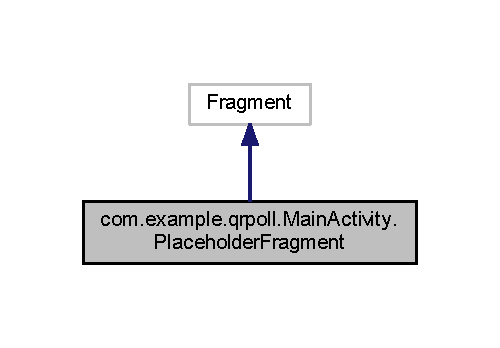
\includegraphics[width=240pt]{classcom_1_1example_1_1qrpoll_1_1_main_activity_1_1_placeholder_fragment__inherit__graph}
\end{center}
\end{figure}


Diagram współpracy dla com.\+example.\+qrpoll.\+Main\+Activity.\+Placeholder\+Fragment\+:\nopagebreak
\begin{figure}[H]
\begin{center}
\leavevmode
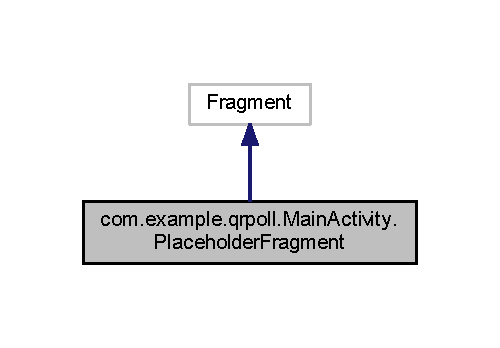
\includegraphics[width=240pt]{classcom_1_1example_1_1qrpoll_1_1_main_activity_1_1_placeholder_fragment__coll__graph}
\end{center}
\end{figure}
\subsection*{Metody publiczne}
\begin{DoxyCompactItemize}
\item 
\hyperlink{classcom_1_1example_1_1qrpoll_1_1_main_activity_1_1_placeholder_fragment_a4c4b85126c7697bf2198e6f860c97ed9}{Placeholder\+Fragment} ()
\item 
View \hyperlink{classcom_1_1example_1_1qrpoll_1_1_main_activity_1_1_placeholder_fragment_aa383980579fc369d3f24a4094afc9316}{on\+Create\+View} (Layout\+Inflater inflater, View\+Group container, Bundle saved\+Instance\+State)
\end{DoxyCompactItemize}


\subsection{Opis szczegółowy}
A placeholder fragment containing a simple view. 

Definicja w linii 208 pliku Main\+Activity.\+java.



\subsection{Dokumentacja konstruktora i destruktora}
\hypertarget{classcom_1_1example_1_1qrpoll_1_1_main_activity_1_1_placeholder_fragment_a4c4b85126c7697bf2198e6f860c97ed9}{\index{com\+::example\+::qrpoll\+::\+Main\+Activity\+::\+Placeholder\+Fragment@{com\+::example\+::qrpoll\+::\+Main\+Activity\+::\+Placeholder\+Fragment}!Placeholder\+Fragment@{Placeholder\+Fragment}}
\index{Placeholder\+Fragment@{Placeholder\+Fragment}!com\+::example\+::qrpoll\+::\+Main\+Activity\+::\+Placeholder\+Fragment@{com\+::example\+::qrpoll\+::\+Main\+Activity\+::\+Placeholder\+Fragment}}
\subsubsection[{Placeholder\+Fragment}]{\setlength{\rightskip}{0pt plus 5cm}com.\+example.\+qrpoll.\+Main\+Activity.\+Placeholder\+Fragment.\+Placeholder\+Fragment (
\begin{DoxyParamCaption}
{}
\end{DoxyParamCaption}
)}}\label{classcom_1_1example_1_1qrpoll_1_1_main_activity_1_1_placeholder_fragment_a4c4b85126c7697bf2198e6f860c97ed9}


Definicja w linii 210 pliku Main\+Activity.\+java.


\begin{DoxyCode}
210                                      \{
211         \}
\end{DoxyCode}


\subsection{Dokumentacja funkcji składowych}
\hypertarget{classcom_1_1example_1_1qrpoll_1_1_main_activity_1_1_placeholder_fragment_aa383980579fc369d3f24a4094afc9316}{\index{com\+::example\+::qrpoll\+::\+Main\+Activity\+::\+Placeholder\+Fragment@{com\+::example\+::qrpoll\+::\+Main\+Activity\+::\+Placeholder\+Fragment}!on\+Create\+View@{on\+Create\+View}}
\index{on\+Create\+View@{on\+Create\+View}!com\+::example\+::qrpoll\+::\+Main\+Activity\+::\+Placeholder\+Fragment@{com\+::example\+::qrpoll\+::\+Main\+Activity\+::\+Placeholder\+Fragment}}
\subsubsection[{on\+Create\+View}]{\setlength{\rightskip}{0pt plus 5cm}View com.\+example.\+qrpoll.\+Main\+Activity.\+Placeholder\+Fragment.\+on\+Create\+View (
\begin{DoxyParamCaption}
\item[{Layout\+Inflater}]{inflater, }
\item[{View\+Group}]{container, }
\item[{Bundle}]{saved\+Instance\+State}
\end{DoxyParamCaption}
)}}\label{classcom_1_1example_1_1qrpoll_1_1_main_activity_1_1_placeholder_fragment_aa383980579fc369d3f24a4094afc9316}


Definicja w linii 214 pliku Main\+Activity.\+java.


\begin{DoxyCode}
215                                            \{
216             View rootView = inflater.inflate(R.layout.fragment\_main, container, \textcolor{keyword}{false});
217             \textcolor{keywordflow}{return} rootView;
218         \}
\end{DoxyCode}


Dokumentacja dla tej klasy została wygenerowana z pliku\+:\begin{DoxyCompactItemize}
\item 
C\+:/\+Users/\+Wodzu/\+Documents/\+Git\+Hub/\+Projekt\+Zespolowy/\+Android Final + dokumentacja/android/qrpoll/src/com/example/qrpoll/\hyperlink{_main_activity_8java}{Main\+Activity.\+java}\end{DoxyCompactItemize}

\hypertarget{classcom_1_1example_1_1qrpoll_1_1_poll}{\section{Dokumentacja klasy com.\+example.\+qrpoll.\+Poll}
\label{classcom_1_1example_1_1qrpoll_1_1_poll}\index{com.\+example.\+qrpoll.\+Poll@{com.\+example.\+qrpoll.\+Poll}}
}


Diagram współpracy dla com.\+example.\+qrpoll.\+Poll\+:\nopagebreak
\begin{figure}[H]
\begin{center}
\leavevmode
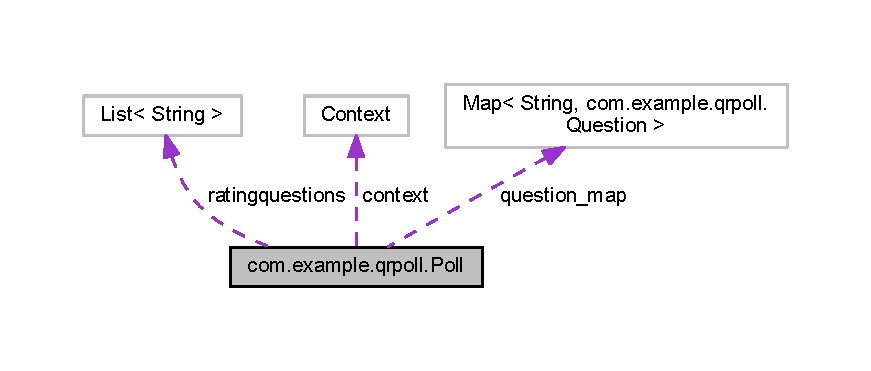
\includegraphics[width=350pt]{classcom_1_1example_1_1qrpoll_1_1_poll__coll__graph}
\end{center}
\end{figure}
\subsection*{Metody publiczne}
\begin{DoxyCompactItemize}
\item 
\hyperlink{classcom_1_1example_1_1qrpoll_1_1_poll_a67b9e49c516a9c614e1e9964f151ed5e}{Poll} (String \hyperlink{classcom_1_1example_1_1qrpoll_1_1_poll_a284d664b1db022d0fe8f089c4cad5ead}{address}, Context \hyperlink{classcom_1_1example_1_1qrpoll_1_1_poll_a22159bb6ccaf5330c7691c47fcb0ea00}{context})  throws J\+S\+O\+N\+Exception
\item 
void \hyperlink{classcom_1_1example_1_1qrpoll_1_1_poll_a18e558fa9d47671bff6fd21eaf7d4a10}{vote} (String pk)
\item 
String \hyperlink{classcom_1_1example_1_1qrpoll_1_1_poll_ac84c3d1747b6eb8d4f43da448de8080f}{get\+Address} ()
\item 
String \hyperlink{classcom_1_1example_1_1qrpoll_1_1_poll_ab6bbc4a6d847d1f6b64543007c3a551c}{get\+Hash\+\_\+id} ()
\item 
String \hyperlink{classcom_1_1example_1_1qrpoll_1_1_poll_af744727f34328a8fec2cb1aba1bc5f66}{get\+Subject} ()
\item 
String \hyperlink{classcom_1_1example_1_1qrpoll_1_1_poll_a4622b5c93daf183b787ecad660a207ad}{get\+Room} ()
\item 
String \hyperlink{classcom_1_1example_1_1qrpoll_1_1_poll_a51e13329a38c4ee0fc09ccac02ae5afe}{get\+Start\+\_\+date} ()
\item 
int \hyperlink{classcom_1_1example_1_1qrpoll_1_1_poll_a6ec1751ddf25a1b00173e1c4f3203458}{get\+Version} ()
\item 
Map$<$ String, \hyperlink{classcom_1_1example_1_1qrpoll_1_1_question}{Question} $>$ \hyperlink{classcom_1_1example_1_1qrpoll_1_1_poll_a505fc3d6479ef24c04adb022acc366c8}{get\+Question\+\_\+map} ()
\end{DoxyCompactItemize}
\subsection*{Atrybuty publiczne}
\begin{DoxyCompactItemize}
\item 
int \hyperlink{classcom_1_1example_1_1qrpoll_1_1_poll_a41aee71def14cf65836f768222a32ba3}{rating\+I\+D} =0
\item 
List$<$ String $>$ \hyperlink{classcom_1_1example_1_1qrpoll_1_1_poll_a357dc2acb9f42f2bee8dd88556551637}{ratingquestions} =new Array\+List$<$String$>$()
\end{DoxyCompactItemize}
\subsection*{Atrybuty prywatne}
\begin{DoxyCompactItemize}
\item 
String \hyperlink{classcom_1_1example_1_1qrpoll_1_1_poll_a284d664b1db022d0fe8f089c4cad5ead}{address}
\item 
String \hyperlink{classcom_1_1example_1_1qrpoll_1_1_poll_acbb2a9859e39f1b1ce48e75c95eb3866}{hash\+\_\+id}
\item 
String \hyperlink{classcom_1_1example_1_1qrpoll_1_1_poll_ac710a3059ee7152dd6aa5e7bea399726}{subject}
\item 
String \hyperlink{classcom_1_1example_1_1qrpoll_1_1_poll_a73035d1fde89a6b4d69cd4e5ee610b8b}{room}
\item 
String \hyperlink{classcom_1_1example_1_1qrpoll_1_1_poll_a43059ae0d84924af4a6f876f31ee26d4}{start\+\_\+date}
\item 
int \hyperlink{classcom_1_1example_1_1qrpoll_1_1_poll_af8617455744b1f5935c9c4042345782c}{version}
\item 
Map$<$ String, \hyperlink{classcom_1_1example_1_1qrpoll_1_1_question}{Question} $>$ \hyperlink{classcom_1_1example_1_1qrpoll_1_1_poll_ac4019650bac8ecbf279808dc4d4dae9b}{question\+\_\+map}
\item 
Context \hyperlink{classcom_1_1example_1_1qrpoll_1_1_poll_a22159bb6ccaf5330c7691c47fcb0ea00}{context}
\end{DoxyCompactItemize}


\subsection{Opis szczegółowy}
Klasa odpowiedzialna za obsluge ankiety\+:wywoluje pobranie ze strony, przypisuje odpowiedzi do pytan, wysyla glosy na serwer

\begin{DoxyAuthor}{Autor}
Piotrek 

Sliwka (poprawki) 
\end{DoxyAuthor}


Definicja w linii 35 pliku Poll.\+java.



\subsection{Dokumentacja konstruktora i destruktora}
\hypertarget{classcom_1_1example_1_1qrpoll_1_1_poll_a67b9e49c516a9c614e1e9964f151ed5e}{\index{com\+::example\+::qrpoll\+::\+Poll@{com\+::example\+::qrpoll\+::\+Poll}!Poll@{Poll}}
\index{Poll@{Poll}!com\+::example\+::qrpoll\+::\+Poll@{com\+::example\+::qrpoll\+::\+Poll}}
\subsubsection[{Poll}]{\setlength{\rightskip}{0pt plus 5cm}com.\+example.\+qrpoll.\+Poll.\+Poll (
\begin{DoxyParamCaption}
\item[{String}]{address, }
\item[{Context}]{context}
\end{DoxyParamCaption}
) throws J\+S\+O\+N\+Exception}}\label{classcom_1_1example_1_1qrpoll_1_1_poll_a67b9e49c516a9c614e1e9964f151ed5e}
Konstruktor,Przetwarzanie danych zawartych w formacie J\+S\+O\+N, laczenie pytan z odpowiedziami 
\begin{DoxyParams}{Parametry}
{\em address} & adres strony z ktorej chcemy pobrac dane \\
\hline
{\em context} & \\
\hline
\end{DoxyParams}

\begin{DoxyExceptions}{Wyjątki}
{\em J\+S\+O\+N\+Exception} & \\
\hline
\end{DoxyExceptions}


Definicja w linii 55 pliku Poll.\+java.


\begin{DoxyCode}
55                                                                     \{
56         
57         
58         StrictMode.ThreadPolicy policy = \textcolor{keyword}{new} StrictMode.ThreadPolicy.Builder().permitAll().build(); 
59         StrictMode.setThreadPolicy(policy);
60         
61         this.address = \hyperlink{classcom_1_1example_1_1qrpoll_1_1_poll_a284d664b1db022d0fe8f089c4cad5ead}{address};
62         this.context = \hyperlink{classcom_1_1example_1_1qrpoll_1_1_poll_a22159bb6ccaf5330c7691c47fcb0ea00}{context};
63         
64         String full\_address = \hyperlink{classcom_1_1example_1_1qrpoll_1_1_poll_a284d664b1db022d0fe8f089c4cad5ead}{address} + \textcolor{stringliteral}{"api/info"};
65         String s = \textcolor{stringliteral}{""};
66         \textcolor{keywordflow}{try} \{
67             s = MyHttpURLConnection.get(full\_address);
68         \} \textcolor{keywordflow}{catch} (Exception404 e) \{
69             System.out.println(\textcolor{stringliteral}{"404!"});
70         \} \textcolor{keywordflow}{catch} (Exception e) \{
71             \textcolor{comment}{// TODO Auto-generated catch block}
72             e.printStackTrace();
73         \}
74         JSONArray array;
75         JSONObject jo;
76         JSONObject jo\_inside;
77         
78         \textcolor{keywordflow}{try}\{
79             array = \textcolor{keyword}{new} JSONArray(s);
80             jo = array.getJSONObject(0);
81             jo\_inside = jo.getJSONObject(\textcolor{stringliteral}{"info"}); 
82             this.hash\_id = jo\_inside.get(\textcolor{stringliteral}{"hash\_id"}).toString();
83             this.subject = jo\_inside.get(\textcolor{stringliteral}{"subject"}).toString();
84             this.room = jo\_inside.get(\textcolor{stringliteral}{"room"}).toString();
85             this.start\_date =  jo\_inside.get(\textcolor{stringliteral}{"time"}).toString();
86         \}\textcolor{keywordflow}{catch}(JSONException e)\{
87             e.printStackTrace();
88         \}
89         
90         
91         full\_address = \hyperlink{classcom_1_1example_1_1qrpoll_1_1_poll_a284d664b1db022d0fe8f089c4cad5ead}{address} + \textcolor{stringliteral}{"api/version"};
92         
93         \textcolor{keywordflow}{try} \{
94             s = MyHttpURLConnection.get(full\_address);
95         \} \textcolor{keywordflow}{catch} (Exception404 e) \{
96             e.printStackTrace();
97         \} \textcolor{keywordflow}{catch} (Exception e) \{
98             e.printStackTrace();
99         \}
100         
101         Log.d(\textcolor{stringliteral}{"moje"}, s);
102             
103 
104         array = \textcolor{keyword}{new} JSONArray(s);
105         jo = array.getJSONObject(0);
106         \hyperlink{classcom_1_1example_1_1qrpoll_1_1_poll_af8617455744b1f5935c9c4042345782c}{version} = Integer.parseInt(jo.get(\textcolor{stringliteral}{"version"}).toString());
107         
108         full\_address = \hyperlink{classcom_1_1example_1_1qrpoll_1_1_poll_a284d664b1db022d0fe8f089c4cad5ead}{address} + \textcolor{stringliteral}{"api/questions"};
109         
110         \textcolor{keywordflow}{try} \{
111             s = MyHttpURLConnection.get(full\_address);
112         \} \textcolor{keywordflow}{catch} (Exception404 e) \{
113             e.printStackTrace();
114         \} \textcolor{keywordflow}{catch} (Exception e) \{
115             e.printStackTrace();
116         \}
117                     
118         array = \textcolor{keyword}{new} JSONArray(s);
119         
120         String pk, question\_text;
121         
122         \hyperlink{classcom_1_1example_1_1qrpoll_1_1_poll_ac4019650bac8ecbf279808dc4d4dae9b}{question\_map} = \textcolor{keyword}{new} HashMap<String,Question>(); 
123         \textcolor{keywordflow}{for}(\textcolor{keywordtype}{int} i =0;i<array.length();i++)\{
124             jo = array.getJSONObject(i);
125             pk = jo.get(\textcolor{stringliteral}{"pk"}).toString(); 
126             jo\_inside = jo.getJSONObject(\textcolor{stringliteral}{"fields"});
127             question\_text = jo\_inside.get(\textcolor{stringliteral}{"question\_text"}).toString();
128             String rating=jo\_inside.get(\textcolor{stringliteral}{"isRating"}).toString();
129             String max=jo\_inside.get(\textcolor{stringliteral}{"question\_choices\_max"}).toString();
130             \textcolor{keywordflow}{if}(rating.equals(\textcolor{stringliteral}{"false"}))\{
131                 question\_map.put(pk,\textcolor{keyword}{new} Question(pk, question\_text,rating,max));
132             \}\textcolor{keywordflow}{else}\{
133                 \hyperlink{classcom_1_1example_1_1qrpoll_1_1_poll_a41aee71def14cf65836f768222a32ba3}{ratingID}=Integer.parseInt(pk);
134             \}
135             
136             
137         \}
138         
139         
140         full\_address = \hyperlink{classcom_1_1example_1_1qrpoll_1_1_poll_a284d664b1db022d0fe8f089c4cad5ead}{address} + \textcolor{stringliteral}{"api/choices"};
141         
142         \textcolor{keywordflow}{try} \{
143             s = MyHttpURLConnection.get(full\_address);
144         \} \textcolor{keywordflow}{catch} (Exception404 e) \{
145             e.printStackTrace();
146         \} \textcolor{keywordflow}{catch} (Exception e) \{
147             e.printStackTrace();
148         \}
149         
150         array = \textcolor{keyword}{new} JSONArray(s);
151         
152         String question\_pk, choice\_text;
153         \textcolor{keywordtype}{int} votes;
154         
155         \textcolor{keywordflow}{for}(\textcolor{keywordtype}{int} i =0;i<array.length();i++)\{
156             jo = array.getJSONObject(i);
157             pk = jo.get(\textcolor{stringliteral}{"pk"}).toString();
158             jo\_inside = jo.getJSONObject(\textcolor{stringliteral}{"fields"});
159             question\_pk = jo\_inside.get(\textcolor{stringliteral}{"question"}).toString();
160             choice\_text = jo\_inside.get(\textcolor{stringliteral}{"choice\_text"}).toString();
161             \textcolor{keywordflow}{if}(!question\_pk.equals(\hyperlink{classcom_1_1example_1_1qrpoll_1_1_poll_a41aee71def14cf65836f768222a32ba3}{ratingID}+\textcolor{stringliteral}{""}))\{           
162             question\_map.get(question\_pk).addChoice(pk, choice\_text);
163             \}\textcolor{keywordflow}{else}\{
164                 ratingquestions.add(pk);
165             \}
166         \}
167                     
168         
169     \}
\end{DoxyCode}


\subsection{Dokumentacja funkcji składowych}
\hypertarget{classcom_1_1example_1_1qrpoll_1_1_poll_ac84c3d1747b6eb8d4f43da448de8080f}{\index{com\+::example\+::qrpoll\+::\+Poll@{com\+::example\+::qrpoll\+::\+Poll}!get\+Address@{get\+Address}}
\index{get\+Address@{get\+Address}!com\+::example\+::qrpoll\+::\+Poll@{com\+::example\+::qrpoll\+::\+Poll}}
\subsubsection[{get\+Address}]{\setlength{\rightskip}{0pt plus 5cm}String com.\+example.\+qrpoll.\+Poll.\+get\+Address (
\begin{DoxyParamCaption}
{}
\end{DoxyParamCaption}
)}}\label{classcom_1_1example_1_1qrpoll_1_1_poll_ac84c3d1747b6eb8d4f43da448de8080f}
Dostep do zmiennych prywatnych \begin{DoxyReturn}{Zwraca}
url spotkania 
\end{DoxyReturn}


Definicja w linii 197 pliku Poll.\+java.


\begin{DoxyCode}
197                                \{
198         \textcolor{keywordflow}{return} \hyperlink{classcom_1_1example_1_1qrpoll_1_1_poll_a284d664b1db022d0fe8f089c4cad5ead}{address};
199     \}
\end{DoxyCode}


Oto graf wywoływań tej funkcji\+:
\nopagebreak
\begin{figure}[H]
\begin{center}
\leavevmode
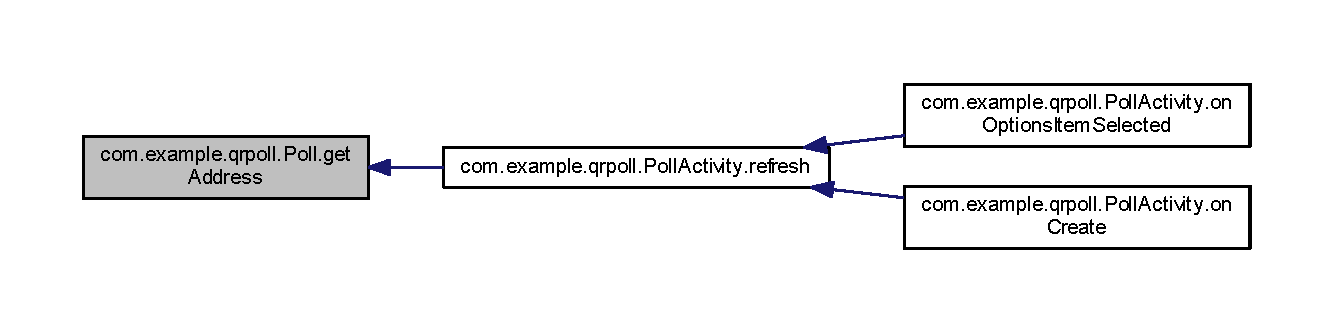
\includegraphics[width=350pt]{classcom_1_1example_1_1qrpoll_1_1_poll_ac84c3d1747b6eb8d4f43da448de8080f_icgraph}
\end{center}
\end{figure}


\hypertarget{classcom_1_1example_1_1qrpoll_1_1_poll_ab6bbc4a6d847d1f6b64543007c3a551c}{\index{com\+::example\+::qrpoll\+::\+Poll@{com\+::example\+::qrpoll\+::\+Poll}!get\+Hash\+\_\+id@{get\+Hash\+\_\+id}}
\index{get\+Hash\+\_\+id@{get\+Hash\+\_\+id}!com\+::example\+::qrpoll\+::\+Poll@{com\+::example\+::qrpoll\+::\+Poll}}
\subsubsection[{get\+Hash\+\_\+id}]{\setlength{\rightskip}{0pt plus 5cm}String com.\+example.\+qrpoll.\+Poll.\+get\+Hash\+\_\+id (
\begin{DoxyParamCaption}
{}
\end{DoxyParamCaption}
)}}\label{classcom_1_1example_1_1qrpoll_1_1_poll_ab6bbc4a6d847d1f6b64543007c3a551c}
Dostep do zmiennych prywatnych \begin{DoxyReturn}{Zwraca}
kod hash spotkania 
\end{DoxyReturn}


Definicja w linii 204 pliku Poll.\+java.


\begin{DoxyCode}
204                                \{
205         \textcolor{keywordflow}{return} \hyperlink{classcom_1_1example_1_1qrpoll_1_1_poll_acbb2a9859e39f1b1ce48e75c95eb3866}{hash\_id};
206     \}
\end{DoxyCode}
\hypertarget{classcom_1_1example_1_1qrpoll_1_1_poll_a505fc3d6479ef24c04adb022acc366c8}{\index{com\+::example\+::qrpoll\+::\+Poll@{com\+::example\+::qrpoll\+::\+Poll}!get\+Question\+\_\+map@{get\+Question\+\_\+map}}
\index{get\+Question\+\_\+map@{get\+Question\+\_\+map}!com\+::example\+::qrpoll\+::\+Poll@{com\+::example\+::qrpoll\+::\+Poll}}
\subsubsection[{get\+Question\+\_\+map}]{\setlength{\rightskip}{0pt plus 5cm}Map$<$String, {\bf Question}$>$ com.\+example.\+qrpoll.\+Poll.\+get\+Question\+\_\+map (
\begin{DoxyParamCaption}
{}
\end{DoxyParamCaption}
)}}\label{classcom_1_1example_1_1qrpoll_1_1_poll_a505fc3d6479ef24c04adb022acc366c8}
Dostep do zmiennych prywatnych, \begin{DoxyReturn}{Zwraca}
mapa zawierajaca pytania z pytania 
\end{DoxyReturn}


Definicja w linii 239 pliku Poll.\+java.


\begin{DoxyCode}
239                                                    \{
240         \textcolor{keywordflow}{return} \hyperlink{classcom_1_1example_1_1qrpoll_1_1_poll_ac4019650bac8ecbf279808dc4d4dae9b}{question\_map};
241     \}
\end{DoxyCode}
\hypertarget{classcom_1_1example_1_1qrpoll_1_1_poll_a4622b5c93daf183b787ecad660a207ad}{\index{com\+::example\+::qrpoll\+::\+Poll@{com\+::example\+::qrpoll\+::\+Poll}!get\+Room@{get\+Room}}
\index{get\+Room@{get\+Room}!com\+::example\+::qrpoll\+::\+Poll@{com\+::example\+::qrpoll\+::\+Poll}}
\subsubsection[{get\+Room}]{\setlength{\rightskip}{0pt plus 5cm}String com.\+example.\+qrpoll.\+Poll.\+get\+Room (
\begin{DoxyParamCaption}
{}
\end{DoxyParamCaption}
)}}\label{classcom_1_1example_1_1qrpoll_1_1_poll_a4622b5c93daf183b787ecad660a207ad}
Dostep do zmiennych prywatnych \begin{DoxyReturn}{Zwraca}
pokoj, w ktorym odbywa sie spotkanie 
\end{DoxyReturn}


Definicja w linii 218 pliku Poll.\+java.


\begin{DoxyCode}
218                             \{
219         \textcolor{keywordflow}{return} \hyperlink{classcom_1_1example_1_1qrpoll_1_1_poll_a73035d1fde89a6b4d69cd4e5ee610b8b}{room};
220     \}
\end{DoxyCode}
\hypertarget{classcom_1_1example_1_1qrpoll_1_1_poll_a51e13329a38c4ee0fc09ccac02ae5afe}{\index{com\+::example\+::qrpoll\+::\+Poll@{com\+::example\+::qrpoll\+::\+Poll}!get\+Start\+\_\+date@{get\+Start\+\_\+date}}
\index{get\+Start\+\_\+date@{get\+Start\+\_\+date}!com\+::example\+::qrpoll\+::\+Poll@{com\+::example\+::qrpoll\+::\+Poll}}
\subsubsection[{get\+Start\+\_\+date}]{\setlength{\rightskip}{0pt plus 5cm}String com.\+example.\+qrpoll.\+Poll.\+get\+Start\+\_\+date (
\begin{DoxyParamCaption}
{}
\end{DoxyParamCaption}
)}}\label{classcom_1_1example_1_1qrpoll_1_1_poll_a51e13329a38c4ee0fc09ccac02ae5afe}
Dostep do zmiennych prywatnych \begin{DoxyReturn}{Zwraca}
poczatek spotkania 
\end{DoxyReturn}


Definicja w linii 225 pliku Poll.\+java.


\begin{DoxyCode}
225                                   \{
226         \textcolor{keywordflow}{return} \hyperlink{classcom_1_1example_1_1qrpoll_1_1_poll_a43059ae0d84924af4a6f876f31ee26d4}{start\_date};
227     \}
\end{DoxyCode}


Oto graf wywoływań tej funkcji\+:
\nopagebreak
\begin{figure}[H]
\begin{center}
\leavevmode
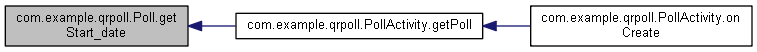
\includegraphics[width=350pt]{classcom_1_1example_1_1qrpoll_1_1_poll_a51e13329a38c4ee0fc09ccac02ae5afe_icgraph}
\end{center}
\end{figure}


\hypertarget{classcom_1_1example_1_1qrpoll_1_1_poll_af744727f34328a8fec2cb1aba1bc5f66}{\index{com\+::example\+::qrpoll\+::\+Poll@{com\+::example\+::qrpoll\+::\+Poll}!get\+Subject@{get\+Subject}}
\index{get\+Subject@{get\+Subject}!com\+::example\+::qrpoll\+::\+Poll@{com\+::example\+::qrpoll\+::\+Poll}}
\subsubsection[{get\+Subject}]{\setlength{\rightskip}{0pt plus 5cm}String com.\+example.\+qrpoll.\+Poll.\+get\+Subject (
\begin{DoxyParamCaption}
{}
\end{DoxyParamCaption}
)}}\label{classcom_1_1example_1_1qrpoll_1_1_poll_af744727f34328a8fec2cb1aba1bc5f66}
Dostep do zmiennych prywatnych \begin{DoxyReturn}{Zwraca}
temat spotkania 
\end{DoxyReturn}


Definicja w linii 211 pliku Poll.\+java.


\begin{DoxyCode}
211                                \{
212         \textcolor{keywordflow}{return} \hyperlink{classcom_1_1example_1_1qrpoll_1_1_poll_ac710a3059ee7152dd6aa5e7bea399726}{subject};
213     \}
\end{DoxyCode}


Oto graf wywoływań tej funkcji\+:
\nopagebreak
\begin{figure}[H]
\begin{center}
\leavevmode
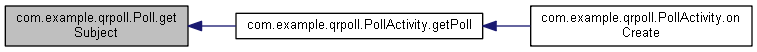
\includegraphics[width=350pt]{classcom_1_1example_1_1qrpoll_1_1_poll_af744727f34328a8fec2cb1aba1bc5f66_icgraph}
\end{center}
\end{figure}


\hypertarget{classcom_1_1example_1_1qrpoll_1_1_poll_a6ec1751ddf25a1b00173e1c4f3203458}{\index{com\+::example\+::qrpoll\+::\+Poll@{com\+::example\+::qrpoll\+::\+Poll}!get\+Version@{get\+Version}}
\index{get\+Version@{get\+Version}!com\+::example\+::qrpoll\+::\+Poll@{com\+::example\+::qrpoll\+::\+Poll}}
\subsubsection[{get\+Version}]{\setlength{\rightskip}{0pt plus 5cm}int com.\+example.\+qrpoll.\+Poll.\+get\+Version (
\begin{DoxyParamCaption}
{}
\end{DoxyParamCaption}
)}}\label{classcom_1_1example_1_1qrpoll_1_1_poll_a6ec1751ddf25a1b00173e1c4f3203458}
Dostep do zmiennych prywatnych \begin{DoxyReturn}{Zwraca}
wersja ankiety 
\end{DoxyReturn}


Definicja w linii 232 pliku Poll.\+java.


\begin{DoxyCode}
232                             \{
233         \textcolor{keywordflow}{return} \hyperlink{classcom_1_1example_1_1qrpoll_1_1_poll_af8617455744b1f5935c9c4042345782c}{version};
234     \}
\end{DoxyCode}


Oto graf wywoływań tej funkcji\+:
\nopagebreak
\begin{figure}[H]
\begin{center}
\leavevmode
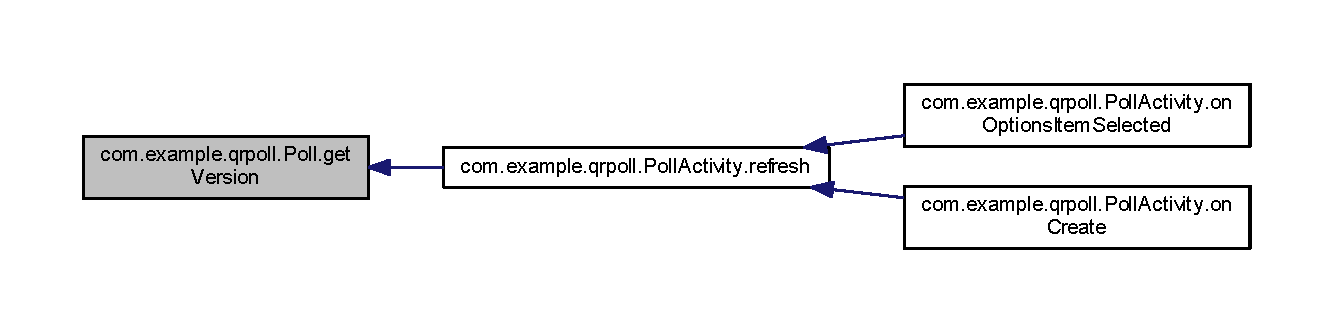
\includegraphics[width=350pt]{classcom_1_1example_1_1qrpoll_1_1_poll_a6ec1751ddf25a1b00173e1c4f3203458_icgraph}
\end{center}
\end{figure}


\hypertarget{classcom_1_1example_1_1qrpoll_1_1_poll_a18e558fa9d47671bff6fd21eaf7d4a10}{\index{com\+::example\+::qrpoll\+::\+Poll@{com\+::example\+::qrpoll\+::\+Poll}!vote@{vote}}
\index{vote@{vote}!com\+::example\+::qrpoll\+::\+Poll@{com\+::example\+::qrpoll\+::\+Poll}}
\subsubsection[{vote}]{\setlength{\rightskip}{0pt plus 5cm}void com.\+example.\+qrpoll.\+Poll.\+vote (
\begin{DoxyParamCaption}
\item[{String}]{pk}
\end{DoxyParamCaption}
)}}\label{classcom_1_1example_1_1qrpoll_1_1_poll_a18e558fa9d47671bff6fd21eaf7d4a10}
Metoda odpowiadajaca za glosowanie 
\begin{DoxyParams}{Parametry}
{\em pk} & numer odpowiedzi na ktora chcemy zaglosowac \\
\hline
\end{DoxyParams}


Definicja w linii 175 pliku Poll.\+java.


\begin{DoxyCode}
175                                \{
176         String full\_address = \hyperlink{classcom_1_1example_1_1qrpoll_1_1_poll_a284d664b1db022d0fe8f089c4cad5ead}{address}+\textcolor{stringliteral}{"api/vote/"}+pk+\textcolor{stringliteral}{"/"};        
177         Log.d(\textcolor{stringliteral}{"moje"},full\_address);
178         \textcolor{keywordflow}{try} \{
179             String response=MyHttpURLConnection.get(full\_address);
180             \textcolor{keywordflow}{if}(response.contains(\textcolor{stringliteral}{"error\(\backslash\)": \(\backslash\)"false\(\backslash\)""}))\{
181                 Toast.makeText(context.getApplicationContext(),\textcolor{stringliteral}{"Zaglosowano"}, Toast.LENGTH\_SHORT).show();
182             \}\textcolor{keywordflow}{else}\{
183                 Toast.makeText(context.getApplicationContext(),\textcolor{stringliteral}{"Blad, wybrano zbyt wiele odpowiedzi"}, Toast
      .LENGTH\_SHORT).show();
184             \}
185         \} \textcolor{keywordflow}{catch} (Exception404 e) \{
186             Toast.makeText(context.getApplicationContext(),\textcolor{stringliteral}{"Nie znaleziono strony"}, Toast.LENGTH\_SHORT)
      .show();
187 
188         \} \textcolor{keywordflow}{catch} (Exception e) \{
189             e.printStackTrace();
190             Toast.makeText(context.getApplicationContext(),\textcolor{stringliteral}{"Blad Polaczenia"}, Toast.LENGTH\_SHORT).show();
191         \}
192     \}
\end{DoxyCode}


\subsection{Dokumentacja atrybutów składowych}
\hypertarget{classcom_1_1example_1_1qrpoll_1_1_poll_a284d664b1db022d0fe8f089c4cad5ead}{\index{com\+::example\+::qrpoll\+::\+Poll@{com\+::example\+::qrpoll\+::\+Poll}!address@{address}}
\index{address@{address}!com\+::example\+::qrpoll\+::\+Poll@{com\+::example\+::qrpoll\+::\+Poll}}
\subsubsection[{address}]{\setlength{\rightskip}{0pt plus 5cm}String com.\+example.\+qrpoll.\+Poll.\+address\hspace{0.3cm}{\ttfamily [private]}}}\label{classcom_1_1example_1_1qrpoll_1_1_poll_a284d664b1db022d0fe8f089c4cad5ead}


Definicja w linii 38 pliku Poll.\+java.

\hypertarget{classcom_1_1example_1_1qrpoll_1_1_poll_a22159bb6ccaf5330c7691c47fcb0ea00}{\index{com\+::example\+::qrpoll\+::\+Poll@{com\+::example\+::qrpoll\+::\+Poll}!context@{context}}
\index{context@{context}!com\+::example\+::qrpoll\+::\+Poll@{com\+::example\+::qrpoll\+::\+Poll}}
\subsubsection[{context}]{\setlength{\rightskip}{0pt plus 5cm}Context com.\+example.\+qrpoll.\+Poll.\+context\hspace{0.3cm}{\ttfamily [private]}}}\label{classcom_1_1example_1_1qrpoll_1_1_poll_a22159bb6ccaf5330c7691c47fcb0ea00}


Definicja w linii 45 pliku Poll.\+java.

\hypertarget{classcom_1_1example_1_1qrpoll_1_1_poll_acbb2a9859e39f1b1ce48e75c95eb3866}{\index{com\+::example\+::qrpoll\+::\+Poll@{com\+::example\+::qrpoll\+::\+Poll}!hash\+\_\+id@{hash\+\_\+id}}
\index{hash\+\_\+id@{hash\+\_\+id}!com\+::example\+::qrpoll\+::\+Poll@{com\+::example\+::qrpoll\+::\+Poll}}
\subsubsection[{hash\+\_\+id}]{\setlength{\rightskip}{0pt plus 5cm}String com.\+example.\+qrpoll.\+Poll.\+hash\+\_\+id\hspace{0.3cm}{\ttfamily [private]}}}\label{classcom_1_1example_1_1qrpoll_1_1_poll_acbb2a9859e39f1b1ce48e75c95eb3866}


Definicja w linii 39 pliku Poll.\+java.

\hypertarget{classcom_1_1example_1_1qrpoll_1_1_poll_ac4019650bac8ecbf279808dc4d4dae9b}{\index{com\+::example\+::qrpoll\+::\+Poll@{com\+::example\+::qrpoll\+::\+Poll}!question\+\_\+map@{question\+\_\+map}}
\index{question\+\_\+map@{question\+\_\+map}!com\+::example\+::qrpoll\+::\+Poll@{com\+::example\+::qrpoll\+::\+Poll}}
\subsubsection[{question\+\_\+map}]{\setlength{\rightskip}{0pt plus 5cm}Map$<$String,{\bf Question}$>$ com.\+example.\+qrpoll.\+Poll.\+question\+\_\+map\hspace{0.3cm}{\ttfamily [private]}}}\label{classcom_1_1example_1_1qrpoll_1_1_poll_ac4019650bac8ecbf279808dc4d4dae9b}


Definicja w linii 44 pliku Poll.\+java.

\hypertarget{classcom_1_1example_1_1qrpoll_1_1_poll_a41aee71def14cf65836f768222a32ba3}{\index{com\+::example\+::qrpoll\+::\+Poll@{com\+::example\+::qrpoll\+::\+Poll}!rating\+I\+D@{rating\+I\+D}}
\index{rating\+I\+D@{rating\+I\+D}!com\+::example\+::qrpoll\+::\+Poll@{com\+::example\+::qrpoll\+::\+Poll}}
\subsubsection[{rating\+I\+D}]{\setlength{\rightskip}{0pt plus 5cm}int com.\+example.\+qrpoll.\+Poll.\+rating\+I\+D =0}}\label{classcom_1_1example_1_1qrpoll_1_1_poll_a41aee71def14cf65836f768222a32ba3}


Definicja w linii 47 pliku Poll.\+java.

\hypertarget{classcom_1_1example_1_1qrpoll_1_1_poll_a357dc2acb9f42f2bee8dd88556551637}{\index{com\+::example\+::qrpoll\+::\+Poll@{com\+::example\+::qrpoll\+::\+Poll}!ratingquestions@{ratingquestions}}
\index{ratingquestions@{ratingquestions}!com\+::example\+::qrpoll\+::\+Poll@{com\+::example\+::qrpoll\+::\+Poll}}
\subsubsection[{ratingquestions}]{\setlength{\rightskip}{0pt plus 5cm}List$<$String$>$ com.\+example.\+qrpoll.\+Poll.\+ratingquestions =new Array\+List$<$String$>$()}}\label{classcom_1_1example_1_1qrpoll_1_1_poll_a357dc2acb9f42f2bee8dd88556551637}


Definicja w linii 48 pliku Poll.\+java.

\hypertarget{classcom_1_1example_1_1qrpoll_1_1_poll_a73035d1fde89a6b4d69cd4e5ee610b8b}{\index{com\+::example\+::qrpoll\+::\+Poll@{com\+::example\+::qrpoll\+::\+Poll}!room@{room}}
\index{room@{room}!com\+::example\+::qrpoll\+::\+Poll@{com\+::example\+::qrpoll\+::\+Poll}}
\subsubsection[{room}]{\setlength{\rightskip}{0pt plus 5cm}String com.\+example.\+qrpoll.\+Poll.\+room\hspace{0.3cm}{\ttfamily [private]}}}\label{classcom_1_1example_1_1qrpoll_1_1_poll_a73035d1fde89a6b4d69cd4e5ee610b8b}


Definicja w linii 41 pliku Poll.\+java.

\hypertarget{classcom_1_1example_1_1qrpoll_1_1_poll_a43059ae0d84924af4a6f876f31ee26d4}{\index{com\+::example\+::qrpoll\+::\+Poll@{com\+::example\+::qrpoll\+::\+Poll}!start\+\_\+date@{start\+\_\+date}}
\index{start\+\_\+date@{start\+\_\+date}!com\+::example\+::qrpoll\+::\+Poll@{com\+::example\+::qrpoll\+::\+Poll}}
\subsubsection[{start\+\_\+date}]{\setlength{\rightskip}{0pt plus 5cm}String com.\+example.\+qrpoll.\+Poll.\+start\+\_\+date\hspace{0.3cm}{\ttfamily [private]}}}\label{classcom_1_1example_1_1qrpoll_1_1_poll_a43059ae0d84924af4a6f876f31ee26d4}


Definicja w linii 42 pliku Poll.\+java.

\hypertarget{classcom_1_1example_1_1qrpoll_1_1_poll_ac710a3059ee7152dd6aa5e7bea399726}{\index{com\+::example\+::qrpoll\+::\+Poll@{com\+::example\+::qrpoll\+::\+Poll}!subject@{subject}}
\index{subject@{subject}!com\+::example\+::qrpoll\+::\+Poll@{com\+::example\+::qrpoll\+::\+Poll}}
\subsubsection[{subject}]{\setlength{\rightskip}{0pt plus 5cm}String com.\+example.\+qrpoll.\+Poll.\+subject\hspace{0.3cm}{\ttfamily [private]}}}\label{classcom_1_1example_1_1qrpoll_1_1_poll_ac710a3059ee7152dd6aa5e7bea399726}


Definicja w linii 40 pliku Poll.\+java.

\hypertarget{classcom_1_1example_1_1qrpoll_1_1_poll_af8617455744b1f5935c9c4042345782c}{\index{com\+::example\+::qrpoll\+::\+Poll@{com\+::example\+::qrpoll\+::\+Poll}!version@{version}}
\index{version@{version}!com\+::example\+::qrpoll\+::\+Poll@{com\+::example\+::qrpoll\+::\+Poll}}
\subsubsection[{version}]{\setlength{\rightskip}{0pt plus 5cm}int com.\+example.\+qrpoll.\+Poll.\+version\hspace{0.3cm}{\ttfamily [private]}}}\label{classcom_1_1example_1_1qrpoll_1_1_poll_af8617455744b1f5935c9c4042345782c}


Definicja w linii 43 pliku Poll.\+java.



Dokumentacja dla tej klasy została wygenerowana z pliku\+:\begin{DoxyCompactItemize}
\item 
C\+:/\+Users/\+Wodzu/\+Documents/\+Git\+Hub/\+Projekt\+Zespolowy/\+Android Final + dokumentacja/android/qrpoll/src/com/example/qrpoll/\hyperlink{_poll_8java}{Poll.\+java}\end{DoxyCompactItemize}

\hypertarget{classcom_1_1example_1_1qrpoll_1_1_poll_activity}{\section{Dokumentacja klasy com.\+example.\+qrpoll.\+Poll\+Activity}
\label{classcom_1_1example_1_1qrpoll_1_1_poll_activity}\index{com.\+example.\+qrpoll.\+Poll\+Activity@{com.\+example.\+qrpoll.\+Poll\+Activity}}
}


Diagram dziedziczenia dla com.\+example.\+qrpoll.\+Poll\+Activity\nopagebreak
\begin{figure}[H]
\begin{center}
\leavevmode
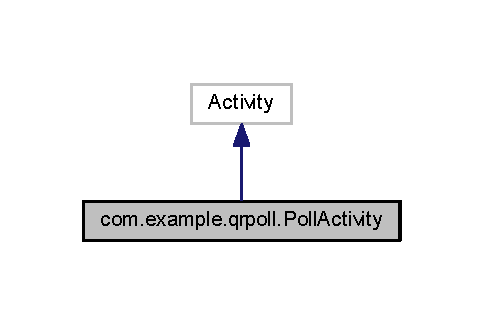
\includegraphics[width=232pt]{classcom_1_1example_1_1qrpoll_1_1_poll_activity__inherit__graph}
\end{center}
\end{figure}


Diagram współpracy dla com.\+example.\+qrpoll.\+Poll\+Activity\+:
\nopagebreak
\begin{figure}[H]
\begin{center}
\leavevmode
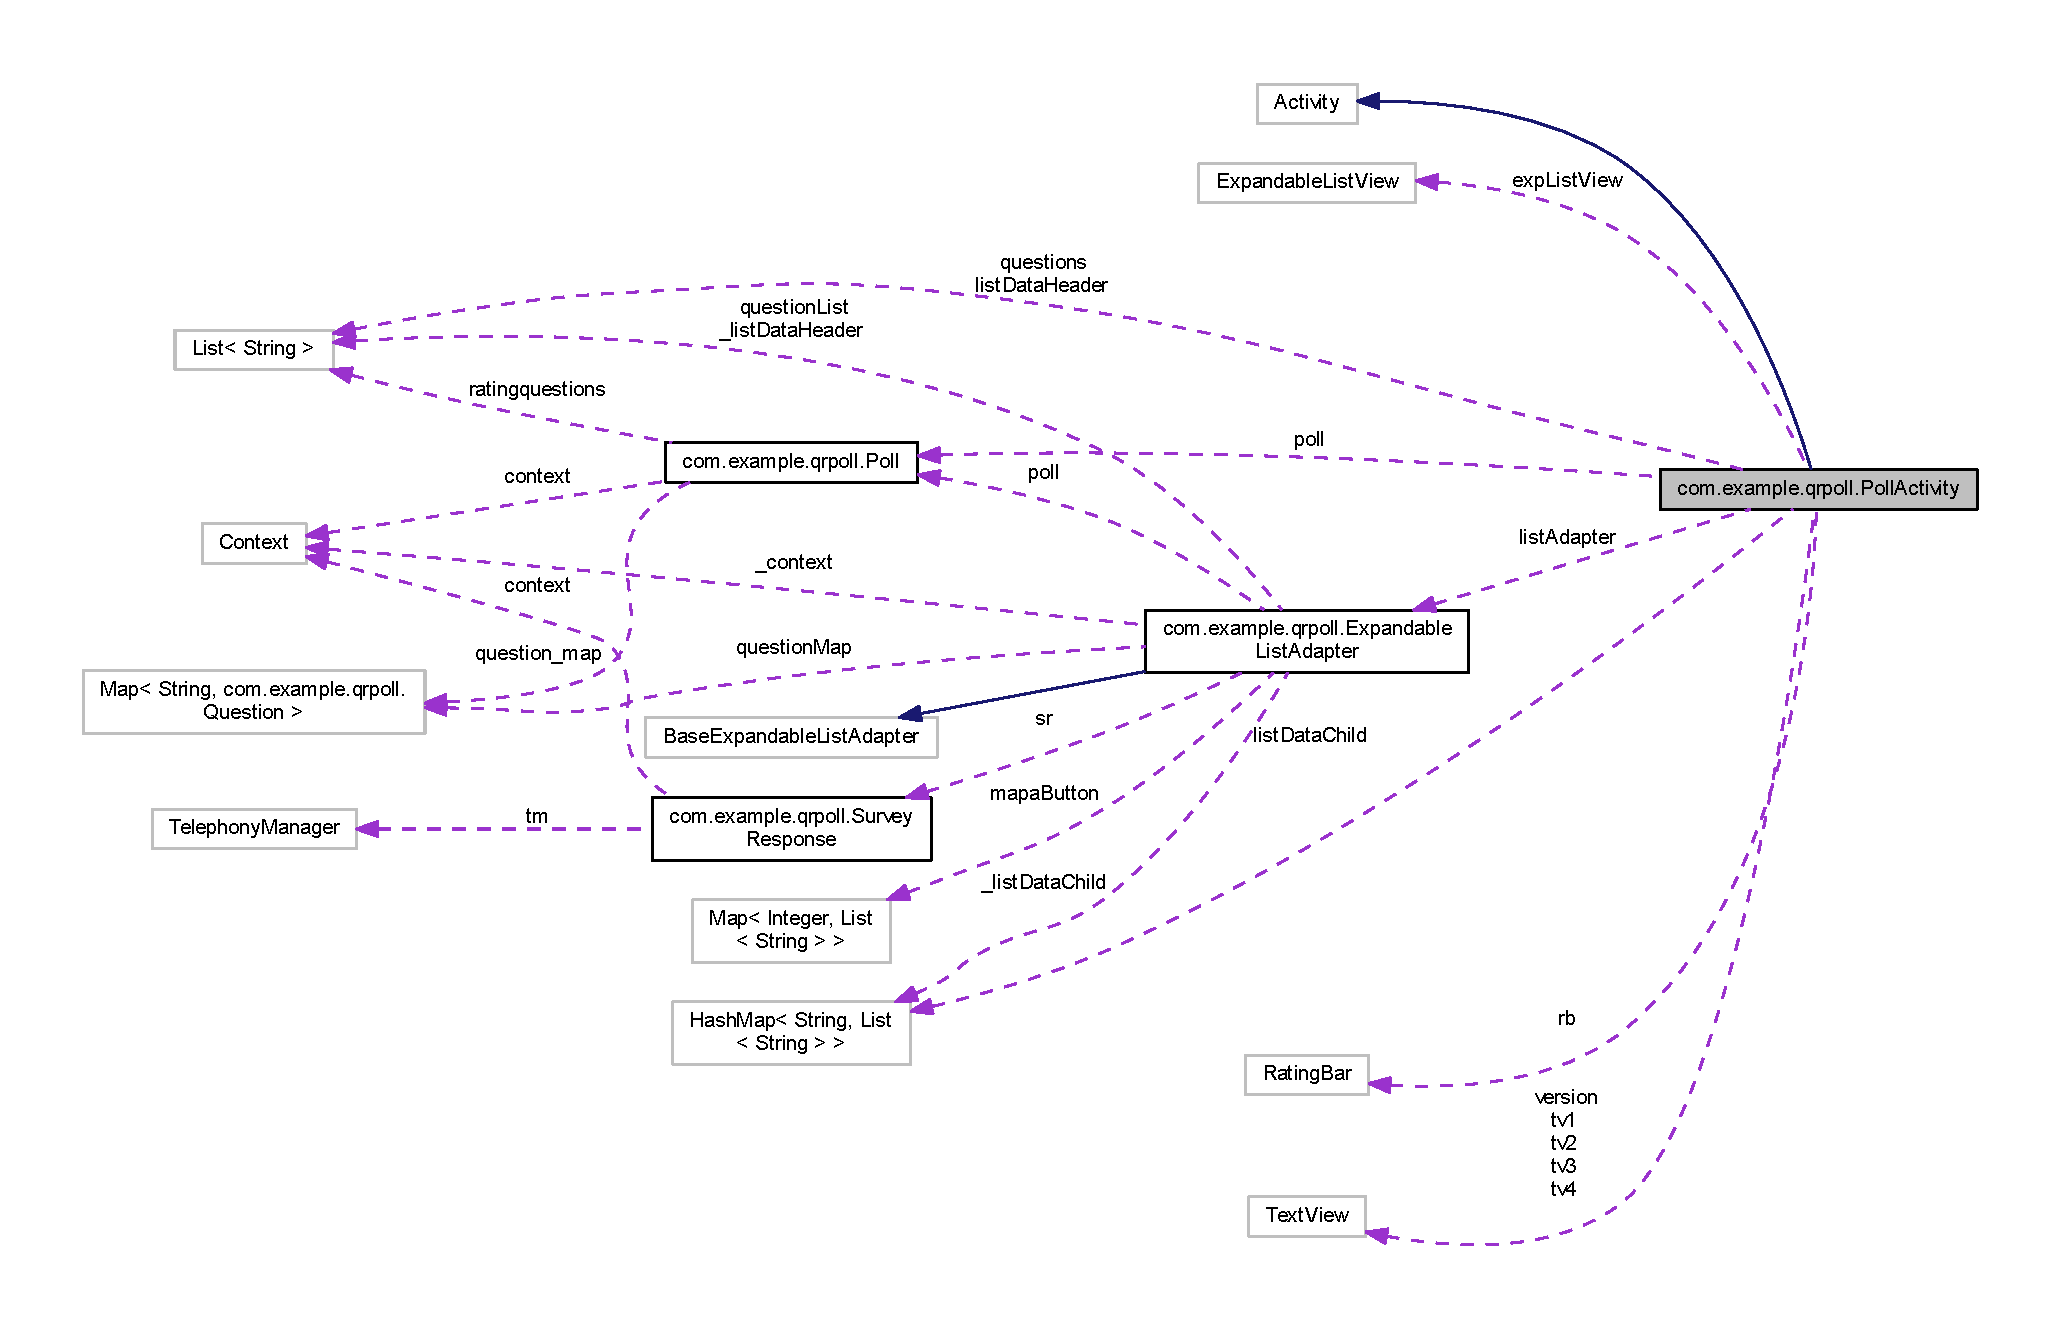
\includegraphics[width=350pt]{classcom_1_1example_1_1qrpoll_1_1_poll_activity__coll__graph}
\end{center}
\end{figure}
\subsection*{Metody publiczne}
\begin{DoxyCompactItemize}
\item 
boolean \hyperlink{classcom_1_1example_1_1qrpoll_1_1_poll_activity_a288dc770b6c610732839043961870030}{on\+Create\+Options\+Menu} (Menu menu)
\item 
boolean \hyperlink{classcom_1_1example_1_1qrpoll_1_1_poll_activity_afc58ce75d02a97bc6e93085c1c23281a}{on\+Options\+Item\+Selected} (Menu\+Item item)
\item 
void \hyperlink{classcom_1_1example_1_1qrpoll_1_1_poll_activity_aa474b030c95c180e2ac43c778c5e0fc9}{get\+Poll} (String url)
\item 
void \hyperlink{classcom_1_1example_1_1qrpoll_1_1_poll_activity_a651f26cfa36578fbf92012881d6a435b}{on\+Back\+Pressed} ()
\item 
void \hyperlink{classcom_1_1example_1_1qrpoll_1_1_poll_activity_a6c59d6b3beb1d5fea9899b0b0cb51e1f}{refresh} ()
\end{DoxyCompactItemize}
\subsection*{Metody chronione}
\begin{DoxyCompactItemize}
\item 
void \hyperlink{classcom_1_1example_1_1qrpoll_1_1_poll_activity_a9982a68e4862d0e8793e0a2e88373589}{on\+Create} (Bundle saved\+Instance\+State)
\end{DoxyCompactItemize}
\subsection*{Atrybuty pakietu}
\begin{DoxyCompactItemize}
\item 
\hyperlink{classcom_1_1example_1_1qrpoll_1_1_expandable_list_adapter}{Expandable\+List\+Adapter} \hyperlink{classcom_1_1example_1_1qrpoll_1_1_poll_activity_aeedb4d35f1bb56db80b834a5c5da4f44}{list\+Adapter}
\item 
Expandable\+List\+View \hyperlink{classcom_1_1example_1_1qrpoll_1_1_poll_activity_a45d9887fce62772f80726024d1775f7d}{exp\+List\+View}
\item 
List$<$ String $>$ \hyperlink{classcom_1_1example_1_1qrpoll_1_1_poll_activity_a62dde3c117f038e463aa7174906f5f7b}{list\+Data\+Header}
\item 
Hash\+Map$<$ String, List$<$ String $>$ $>$ \hyperlink{classcom_1_1example_1_1qrpoll_1_1_poll_activity_ab607bec81e729232d72cee9db8ffdc73}{list\+Data\+Child}
\end{DoxyCompactItemize}
\subsection*{Metody prywatne}
\begin{DoxyCompactItemize}
\item 
void \hyperlink{classcom_1_1example_1_1qrpoll_1_1_poll_activity_a1081f69211873eaf38c422ea12c769f0}{prepare\+List\+Data} ()
\end{DoxyCompactItemize}
\subsection*{Atrybuty prywatne}
\begin{DoxyCompactItemize}
\item 
List$<$ String $>$ \hyperlink{classcom_1_1example_1_1qrpoll_1_1_poll_activity_ae9caea6dcd77802d9edc7f86ace0fc5c}{questions}
\item 
Text\+View \hyperlink{classcom_1_1example_1_1qrpoll_1_1_poll_activity_a7928323c2d0f40aa25420488718de309}{tv1}
\item 
Text\+View \hyperlink{classcom_1_1example_1_1qrpoll_1_1_poll_activity_a48f7da0dc1da430cd5ac90a8376cad70}{tv2}
\item 
Text\+View \hyperlink{classcom_1_1example_1_1qrpoll_1_1_poll_activity_a70708751ea7eb8a32569447a087471b8}{tv3}
\item 
Text\+View \hyperlink{classcom_1_1example_1_1qrpoll_1_1_poll_activity_a32c7797e7d6cdf269f9449cfdb635438}{tv4}
\item 
Text\+View \hyperlink{classcom_1_1example_1_1qrpoll_1_1_poll_activity_a4fbbfc95809c5aa0bf9916316730a992}{version}
\item 
int \hyperlink{classcom_1_1example_1_1qrpoll_1_1_poll_activity_a0cb80128cd6ae3abb14437dbcf82f876}{back\+Button\+Count} =0
\item 
Rating\+Bar \hyperlink{classcom_1_1example_1_1qrpoll_1_1_poll_activity_a3c2b3e0864209b0253263a7af2642a13}{rb}
\item 
\hyperlink{classcom_1_1example_1_1qrpoll_1_1_poll}{Poll} \hyperlink{classcom_1_1example_1_1qrpoll_1_1_poll_activity_accbd807fe57852d64377c5a96401c376}{poll} = null
\end{DoxyCompactItemize}


\subsection{Opis szczegółowy}
Glowne activity aplikacji, odpowiada za wyswietlanie informacji, pytan wraz z odpowiedziami i mozliwosci glosowania \begin{DoxyAuthor}{Autor}
Piotrek, Sliwka 
\end{DoxyAuthor}


Definicja w linii 40 pliku Poll\+Activity.\+java.



\subsection{Dokumentacja funkcji składowych}
\hypertarget{classcom_1_1example_1_1qrpoll_1_1_poll_activity_aa474b030c95c180e2ac43c778c5e0fc9}{\index{com\+::example\+::qrpoll\+::\+Poll\+Activity@{com\+::example\+::qrpoll\+::\+Poll\+Activity}!get\+Poll@{get\+Poll}}
\index{get\+Poll@{get\+Poll}!com\+::example\+::qrpoll\+::\+Poll\+Activity@{com\+::example\+::qrpoll\+::\+Poll\+Activity}}
\subsubsection[{get\+Poll}]{\setlength{\rightskip}{0pt plus 5cm}void com.\+example.\+qrpoll.\+Poll\+Activity.\+get\+Poll (
\begin{DoxyParamCaption}
\item[{String}]{url}
\end{DoxyParamCaption}
)}}\label{classcom_1_1example_1_1qrpoll_1_1_poll_activity_aa474b030c95c180e2ac43c778c5e0fc9}
tworzy nowa ankiete wg podanego url, ustawia odpowiednie informacje na komponentach 
\begin{DoxyParams}{Parametry}
{\em url} & -\/ adres do ankiety np\+: \href{http://loony-waters-2513.herokuapp.com/qrpolls/meeting/b9ffd9db1af0b14ed74e92e8d3273f3e/}{\tt http\+://loony-\/waters-\/2513.\+herokuapp.\+com/qrpolls/meeting/b9ffd9db1af0b14ed74e92e8d3273f3e/} \\
\hline
\end{DoxyParams}


Definicja w linii 234 pliku Poll\+Activity.\+java.


\begin{DoxyCode}
234                                    \{
235         \textcolor{keywordflow}{try} \{
236             \hyperlink{classcom_1_1example_1_1qrpoll_1_1_poll_activity_accbd807fe57852d64377c5a96401c376}{poll} = \textcolor{keyword}{new} Poll(url,getApplicationContext());
237         \} \textcolor{keywordflow}{catch} (JSONException e) \{
238             Toast.makeText(getApplicationContext(),
239                     \textcolor{stringliteral}{"Blad ankiety"}, Toast.LENGTH\_SHORT).show();
240             e.printStackTrace();
241             \textcolor{keywordflow}{return};
242         \}
243         \hyperlink{classcom_1_1example_1_1qrpoll_1_1_poll_activity_ae9caea6dcd77802d9edc7f86ace0fc5c}{questions}=\textcolor{keyword}{new} ArrayList<String>();
244         Map<String,Question> questionMap=this.poll.getQuestion\_map();
245         \textcolor{keywordflow}{for}(String key:questionMap.keySet())\{
246             Question q=questionMap.get(key);
247             
248             questions.add(q.getQuestion\_text() +\textcolor{stringliteral}{"   Max: "}+ q.getMax());
249             
250         \}
251         tv1.setText(poll.getSubject());
252         tv2.setText(poll.getHash\_id());
253         tv3.setText(poll.getStart\_date());
254         tv4.setText(poll.getRoom());
255         version.setText(\textcolor{stringliteral}{"Version: "}+poll.getVersion());
256         SqlHandler sql=\textcolor{keyword}{new} SqlHandler(getApplication());
257         sql.open();
258         sql.insertSpotkania(poll.getHash\_id(), \hyperlink{classcom_1_1example_1_1qrpoll_1_1_poll_activity_accbd807fe57852d64377c5a96401c376}{poll}.\hyperlink{classcom_1_1example_1_1qrpoll_1_1_poll_af744727f34328a8fec2cb1aba1bc5f66}{getSubject}(), poll.getRoom(), 
      \hyperlink{classcom_1_1example_1_1qrpoll_1_1_poll_activity_accbd807fe57852d64377c5a96401c376}{poll}.\hyperlink{classcom_1_1example_1_1qrpoll_1_1_poll_a51e13329a38c4ee0fc09ccac02ae5afe}{getStart\_date}());
259         sql.close();
260         \}
\end{DoxyCode}


Oto graf wywołań dla tej funkcji\+:
\nopagebreak
\begin{figure}[H]
\begin{center}
\leavevmode
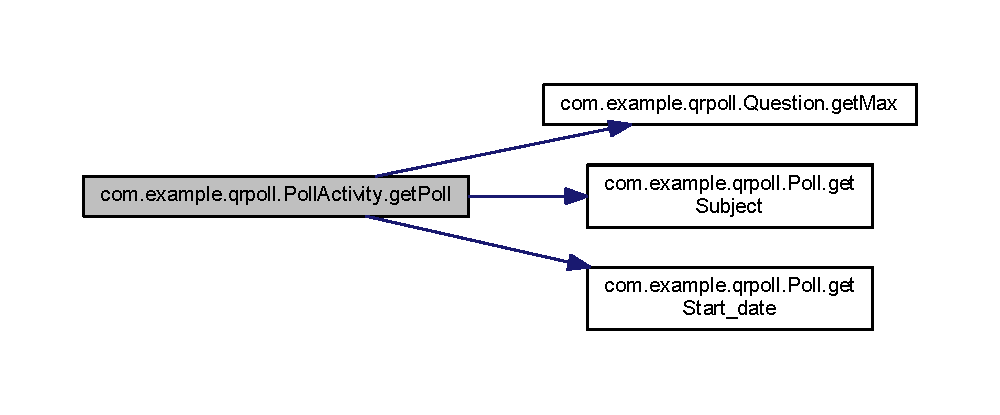
\includegraphics[width=350pt]{classcom_1_1example_1_1qrpoll_1_1_poll_activity_aa474b030c95c180e2ac43c778c5e0fc9_cgraph}
\end{center}
\end{figure}




Oto graf wywoływań tej funkcji\+:
\nopagebreak
\begin{figure}[H]
\begin{center}
\leavevmode
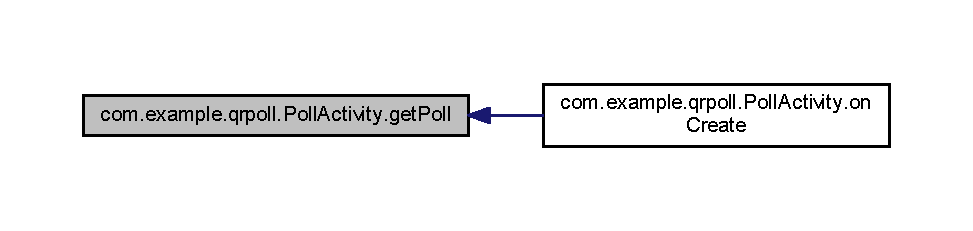
\includegraphics[width=350pt]{classcom_1_1example_1_1qrpoll_1_1_poll_activity_aa474b030c95c180e2ac43c778c5e0fc9_icgraph}
\end{center}
\end{figure}


\hypertarget{classcom_1_1example_1_1qrpoll_1_1_poll_activity_a651f26cfa36578fbf92012881d6a435b}{\index{com\+::example\+::qrpoll\+::\+Poll\+Activity@{com\+::example\+::qrpoll\+::\+Poll\+Activity}!on\+Back\+Pressed@{on\+Back\+Pressed}}
\index{on\+Back\+Pressed@{on\+Back\+Pressed}!com\+::example\+::qrpoll\+::\+Poll\+Activity@{com\+::example\+::qrpoll\+::\+Poll\+Activity}}
\subsubsection[{on\+Back\+Pressed}]{\setlength{\rightskip}{0pt plus 5cm}void com.\+example.\+qrpoll.\+Poll\+Activity.\+on\+Back\+Pressed (
\begin{DoxyParamCaption}
{}
\end{DoxyParamCaption}
)}}\label{classcom_1_1example_1_1qrpoll_1_1_poll_activity_a651f26cfa36578fbf92012881d6a435b}
metoda wywolywana przy nacisnieciu przycisku back, przy dwukrotnym nacisnieciu zamyka aplikacje 

Definicja w linii 265 pliku Poll\+Activity.\+java.


\begin{DoxyCode}
265                                 \{
266         
267         \textcolor{keywordflow}{if}(\hyperlink{classcom_1_1example_1_1qrpoll_1_1_poll_activity_a0cb80128cd6ae3abb14437dbcf82f876}{backButtonCount}>=1)\{
268             finish();
269         \}\textcolor{keywordflow}{else}\{
270             Toast.makeText(getApplicationContext(),
271                     \textcolor{stringliteral}{"Nacisnij jeszcze raz back aby wyjsc z aplikacji"}, Toast.LENGTH\_SHORT).show();
272             \hyperlink{classcom_1_1example_1_1qrpoll_1_1_poll_activity_a0cb80128cd6ae3abb14437dbcf82f876}{backButtonCount}++;
273         \}
274         
275             
276     \}
\end{DoxyCode}
\hypertarget{classcom_1_1example_1_1qrpoll_1_1_poll_activity_a9982a68e4862d0e8793e0a2e88373589}{\index{com\+::example\+::qrpoll\+::\+Poll\+Activity@{com\+::example\+::qrpoll\+::\+Poll\+Activity}!on\+Create@{on\+Create}}
\index{on\+Create@{on\+Create}!com\+::example\+::qrpoll\+::\+Poll\+Activity@{com\+::example\+::qrpoll\+::\+Poll\+Activity}}
\subsubsection[{on\+Create}]{\setlength{\rightskip}{0pt plus 5cm}void com.\+example.\+qrpoll.\+Poll\+Activity.\+on\+Create (
\begin{DoxyParamCaption}
\item[{Bundle}]{saved\+Instance\+State}
\end{DoxyParamCaption}
)\hspace{0.3cm}{\ttfamily [protected]}}}\label{classcom_1_1example_1_1qrpoll_1_1_poll_activity_a9982a68e4862d0e8793e0a2e88373589}
ustawienie wygladu okna, przypisanie akcji do gwiazdek 

Definicja w linii 106 pliku Poll\+Activity.\+java.


\begin{DoxyCode}
106                                                        \{
107         super.onCreate(savedInstanceState);
108         this.requestWindowFeature(Window.FEATURE\_NO\_TITLE);
109         this.getWindow().setFlags(WindowManager.LayoutParams.FLAG\_FULLSCREEN, WindowManager.LayoutParams.
      FLAG\_FULLSCREEN);
110         setContentView(R.layout.activity\_poll);
111         
112         \hyperlink{classcom_1_1example_1_1qrpoll_1_1_poll_activity_a45d9887fce62772f80726024d1775f7d}{expListView} = (ExpandableListView) findViewById(R.id.lvExp);
113         \hyperlink{classcom_1_1example_1_1qrpoll_1_1_poll_activity_a7928323c2d0f40aa25420488718de309}{tv1}=(TextView)findViewById(R.id.textView1);
114         \hyperlink{classcom_1_1example_1_1qrpoll_1_1_poll_activity_a48f7da0dc1da430cd5ac90a8376cad70}{tv2}=(TextView)findViewById(R.id.textView2);
115         \hyperlink{classcom_1_1example_1_1qrpoll_1_1_poll_activity_a70708751ea7eb8a32569447a087471b8}{tv3}=(TextView)findViewById(R.id.textView3);
116         \hyperlink{classcom_1_1example_1_1qrpoll_1_1_poll_activity_a32c7797e7d6cdf269f9449cfdb635438}{tv4}=(TextView)findViewById(R.id.textView4);
117         \hyperlink{classcom_1_1example_1_1qrpoll_1_1_poll_activity_a4fbbfc95809c5aa0bf9916316730a992}{version}=(TextView)findViewById(R.id.poll\_textViewVersionLabel);
118         
119         \hyperlink{classcom_1_1example_1_1qrpoll_1_1_poll_activity_a3c2b3e0864209b0253263a7af2642a13}{rb}=(RatingBar)findViewById(R.id.ratingBar1);
120         
121         rb.setOnRatingBarChangeListener(\textcolor{keyword}{new} OnRatingBarChangeListener() \{
122             \textcolor{keyword}{public} \textcolor{keywordtype}{void} onRatingChanged(RatingBar ratingBar, \textcolor{keywordtype}{float} rating,
123                     \textcolor{keywordtype}{boolean} fromUser) \{
124                 \textcolor{keywordtype}{int} rate=(int)(2*rating);
125                 AboutDevice sr=\textcolor{keyword}{new} AboutDevice(getApplicationContext());
126                 \textcolor{keywordflow}{if}(\hyperlink{classcom_1_1example_1_1qrpoll_1_1_poll_activity_a4fbbfc95809c5aa0bf9916316730a992}{version}.getText().equals(\textcolor{stringliteral}{"1"}))\{
127                 \textcolor{keywordflow}{switch}(rate)\{
128                 \textcolor{keywordflow}{case} 0:
129                     poll.vote(sr.createIdToSend()+\textcolor{stringliteral}{"/"}+\hyperlink{classcom_1_1example_1_1qrpoll_1_1_poll_activity_accbd807fe57852d64377c5a96401c376}{poll}.\hyperlink{classcom_1_1example_1_1qrpoll_1_1_poll_a357dc2acb9f42f2bee8dd88556551637}{ratingquestions}.get(10));
130                     
131                     \textcolor{keywordflow}{break};
132                 \textcolor{keywordflow}{case} 1:
133                     poll.vote(sr.createIdToSend()+\textcolor{stringliteral}{"/"}+\hyperlink{classcom_1_1example_1_1qrpoll_1_1_poll_activity_accbd807fe57852d64377c5a96401c376}{poll}.\hyperlink{classcom_1_1example_1_1qrpoll_1_1_poll_a357dc2acb9f42f2bee8dd88556551637}{ratingquestions}.get(9));
134                     \textcolor{keywordflow}{break};
135                 \textcolor{keywordflow}{case} 2:
136                     poll.vote(sr.createIdToSend()+\textcolor{stringliteral}{"/"}+\hyperlink{classcom_1_1example_1_1qrpoll_1_1_poll_activity_accbd807fe57852d64377c5a96401c376}{poll}.\hyperlink{classcom_1_1example_1_1qrpoll_1_1_poll_a357dc2acb9f42f2bee8dd88556551637}{ratingquestions}.get(8));
137                     \textcolor{keywordflow}{break};
138                 \textcolor{keywordflow}{case} 3:
139                     poll.vote(sr.createIdToSend()+\textcolor{stringliteral}{"/"}+\hyperlink{classcom_1_1example_1_1qrpoll_1_1_poll_activity_accbd807fe57852d64377c5a96401c376}{poll}.\hyperlink{classcom_1_1example_1_1qrpoll_1_1_poll_a357dc2acb9f42f2bee8dd88556551637}{ratingquestions}.get(7));
140                     \textcolor{keywordflow}{break};
141                 \textcolor{keywordflow}{case} 4:
142                     poll.vote(sr.createIdToSend()+\textcolor{stringliteral}{"/"}+\hyperlink{classcom_1_1example_1_1qrpoll_1_1_poll_activity_accbd807fe57852d64377c5a96401c376}{poll}.\hyperlink{classcom_1_1example_1_1qrpoll_1_1_poll_a357dc2acb9f42f2bee8dd88556551637}{ratingquestions}.get(6));
143                     \textcolor{keywordflow}{break};
144                 \textcolor{keywordflow}{case} 5:
145                     poll.vote(sr.createIdToSend()+\textcolor{stringliteral}{"/"}+\hyperlink{classcom_1_1example_1_1qrpoll_1_1_poll_activity_accbd807fe57852d64377c5a96401c376}{poll}.\hyperlink{classcom_1_1example_1_1qrpoll_1_1_poll_a357dc2acb9f42f2bee8dd88556551637}{ratingquestions}.get(5));
146                     \textcolor{keywordflow}{break};
147                 \textcolor{keywordflow}{case} 6:
148                     poll.vote(sr.createIdToSend()+\textcolor{stringliteral}{"/"}+\hyperlink{classcom_1_1example_1_1qrpoll_1_1_poll_activity_accbd807fe57852d64377c5a96401c376}{poll}.\hyperlink{classcom_1_1example_1_1qrpoll_1_1_poll_a357dc2acb9f42f2bee8dd88556551637}{ratingquestions}.get(4));
149                     \textcolor{keywordflow}{break};
150                 \textcolor{keywordflow}{case} 7:
151                     poll.vote(sr.createIdToSend()+\textcolor{stringliteral}{"/"}+\hyperlink{classcom_1_1example_1_1qrpoll_1_1_poll_activity_accbd807fe57852d64377c5a96401c376}{poll}.\hyperlink{classcom_1_1example_1_1qrpoll_1_1_poll_a357dc2acb9f42f2bee8dd88556551637}{ratingquestions}.get(3));
152                     \textcolor{keywordflow}{break};
153                 \textcolor{keywordflow}{case} 8:
154                     poll.vote(sr.createIdToSend()+\textcolor{stringliteral}{"/"}+\hyperlink{classcom_1_1example_1_1qrpoll_1_1_poll_activity_accbd807fe57852d64377c5a96401c376}{poll}.\hyperlink{classcom_1_1example_1_1qrpoll_1_1_poll_a357dc2acb9f42f2bee8dd88556551637}{ratingquestions}.get(2));
155                     \textcolor{keywordflow}{break};
156                 \textcolor{keywordflow}{case} 9:
157                     poll.vote(sr.createIdToSend()+\textcolor{stringliteral}{"/"}+\hyperlink{classcom_1_1example_1_1qrpoll_1_1_poll_activity_accbd807fe57852d64377c5a96401c376}{poll}.\hyperlink{classcom_1_1example_1_1qrpoll_1_1_poll_a357dc2acb9f42f2bee8dd88556551637}{ratingquestions}.get(1));
158                     \textcolor{keywordflow}{break};
159                 \textcolor{keywordflow}{case} 10:
160                     poll.vote(sr.createIdToSend()+\textcolor{stringliteral}{"/"}+\hyperlink{classcom_1_1example_1_1qrpoll_1_1_poll_activity_accbd807fe57852d64377c5a96401c376}{poll}.\hyperlink{classcom_1_1example_1_1qrpoll_1_1_poll_a357dc2acb9f42f2bee8dd88556551637}{ratingquestions}.get(0));
161                     \textcolor{keywordflow}{break};
162                 \}\}\textcolor{keywordflow}{else}\{
163                     \textcolor{keywordflow}{switch}(rate)\{
164                     \textcolor{keywordflow}{case} 0:
165                         poll.vote(sr.createIdToSend()+\textcolor{stringliteral}{"/"}+\hyperlink{classcom_1_1example_1_1qrpoll_1_1_poll_activity_accbd807fe57852d64377c5a96401c376}{poll}.
      \hyperlink{classcom_1_1example_1_1qrpoll_1_1_poll_a357dc2acb9f42f2bee8dd88556551637}{ratingquestions}.get(0));
166                         
167                         \textcolor{keywordflow}{break};
168                     \textcolor{keywordflow}{case} 1:
169                         poll.vote(sr.createIdToSend()+\textcolor{stringliteral}{"/"}+\hyperlink{classcom_1_1example_1_1qrpoll_1_1_poll_activity_accbd807fe57852d64377c5a96401c376}{poll}.
      \hyperlink{classcom_1_1example_1_1qrpoll_1_1_poll_a357dc2acb9f42f2bee8dd88556551637}{ratingquestions}.get(1));
170                         \textcolor{keywordflow}{break};
171                     \textcolor{keywordflow}{case} 2:
172                         poll.vote(sr.createIdToSend()+\textcolor{stringliteral}{"/"}+\hyperlink{classcom_1_1example_1_1qrpoll_1_1_poll_activity_accbd807fe57852d64377c5a96401c376}{poll}.
      \hyperlink{classcom_1_1example_1_1qrpoll_1_1_poll_a357dc2acb9f42f2bee8dd88556551637}{ratingquestions}.get(2));
173                         \textcolor{keywordflow}{break};
174                     \textcolor{keywordflow}{case} 3:
175                         poll.vote(sr.createIdToSend()+\textcolor{stringliteral}{"/"}+\hyperlink{classcom_1_1example_1_1qrpoll_1_1_poll_activity_accbd807fe57852d64377c5a96401c376}{poll}.
      \hyperlink{classcom_1_1example_1_1qrpoll_1_1_poll_a357dc2acb9f42f2bee8dd88556551637}{ratingquestions}.get(3));
176                         \textcolor{keywordflow}{break};
177                     \textcolor{keywordflow}{case} 4:
178                         poll.vote(sr.createIdToSend()+\textcolor{stringliteral}{"/"}+\hyperlink{classcom_1_1example_1_1qrpoll_1_1_poll_activity_accbd807fe57852d64377c5a96401c376}{poll}.
      \hyperlink{classcom_1_1example_1_1qrpoll_1_1_poll_a357dc2acb9f42f2bee8dd88556551637}{ratingquestions}.get(4));
179                         \textcolor{keywordflow}{break};
180                     \textcolor{keywordflow}{case} 5:
181                         poll.vote(sr.createIdToSend()+\textcolor{stringliteral}{"/"}+\hyperlink{classcom_1_1example_1_1qrpoll_1_1_poll_activity_accbd807fe57852d64377c5a96401c376}{poll}.
      \hyperlink{classcom_1_1example_1_1qrpoll_1_1_poll_a357dc2acb9f42f2bee8dd88556551637}{ratingquestions}.get(5));
182                         \textcolor{keywordflow}{break};
183                     \textcolor{keywordflow}{case} 6:
184                         poll.vote(sr.createIdToSend()+\textcolor{stringliteral}{"/"}+\hyperlink{classcom_1_1example_1_1qrpoll_1_1_poll_activity_accbd807fe57852d64377c5a96401c376}{poll}.
      \hyperlink{classcom_1_1example_1_1qrpoll_1_1_poll_a357dc2acb9f42f2bee8dd88556551637}{ratingquestions}.get(6));
185                         \textcolor{keywordflow}{break};
186                     \textcolor{keywordflow}{case} 7:
187                         poll.vote(sr.createIdToSend()+\textcolor{stringliteral}{"/"}+\hyperlink{classcom_1_1example_1_1qrpoll_1_1_poll_activity_accbd807fe57852d64377c5a96401c376}{poll}.
      \hyperlink{classcom_1_1example_1_1qrpoll_1_1_poll_a357dc2acb9f42f2bee8dd88556551637}{ratingquestions}.get(7));
188                         \textcolor{keywordflow}{break};
189                     \textcolor{keywordflow}{case} 8:
190                         poll.vote(sr.createIdToSend()+\textcolor{stringliteral}{"/"}+\hyperlink{classcom_1_1example_1_1qrpoll_1_1_poll_activity_accbd807fe57852d64377c5a96401c376}{poll}.
      \hyperlink{classcom_1_1example_1_1qrpoll_1_1_poll_a357dc2acb9f42f2bee8dd88556551637}{ratingquestions}.get(8));
191                         \textcolor{keywordflow}{break};
192                     \textcolor{keywordflow}{case} 9:
193                         poll.vote(sr.createIdToSend()+\textcolor{stringliteral}{"/"}+\hyperlink{classcom_1_1example_1_1qrpoll_1_1_poll_activity_accbd807fe57852d64377c5a96401c376}{poll}.
      \hyperlink{classcom_1_1example_1_1qrpoll_1_1_poll_a357dc2acb9f42f2bee8dd88556551637}{ratingquestions}.get(9));
194                         \textcolor{keywordflow}{break};
195                     \textcolor{keywordflow}{case} 10:
196                         poll.vote(sr.createIdToSend()+\textcolor{stringliteral}{"/"}+\hyperlink{classcom_1_1example_1_1qrpoll_1_1_poll_activity_accbd807fe57852d64377c5a96401c376}{poll}.
      \hyperlink{classcom_1_1example_1_1qrpoll_1_1_poll_a357dc2acb9f42f2bee8dd88556551637}{ratingquestions}.get(10));
197                         \textcolor{keywordflow}{break};
198                     \}   
199                 \}
200             \}
201         \});
202         
203         Intent intent = getIntent();
204         String url = intent.getStringExtra(\textcolor{stringliteral}{"scanResult"});
205         url = \textcolor{stringliteral}{"http://"}+url;
206         
207         \hyperlink{classcom_1_1example_1_1qrpoll_1_1_poll_activity_aa474b030c95c180e2ac43c778c5e0fc9}{getPoll}(url);
208         \textcolor{keywordflow}{try}\{
209         \hyperlink{classcom_1_1example_1_1qrpoll_1_1_poll_activity_a1081f69211873eaf38c422ea12c769f0}{prepareListData}();
210     
211         \hyperlink{classcom_1_1example_1_1qrpoll_1_1_poll_activity_aeedb4d35f1bb56db80b834a5c5da4f44}{listAdapter}=\textcolor{keyword}{new} ExpandableListAdapter(\textcolor{keyword}{this},\hyperlink{classcom_1_1example_1_1qrpoll_1_1_poll_activity_a62dde3c117f038e463aa7174906f5f7b}{listDataHeader},
      \hyperlink{classcom_1_1example_1_1qrpoll_1_1_poll_activity_ab607bec81e729232d72cee9db8ffdc73}{listDataChild},\hyperlink{classcom_1_1example_1_1qrpoll_1_1_poll_activity_accbd807fe57852d64377c5a96401c376}{poll});
212         expListView.setAdapter(\hyperlink{classcom_1_1example_1_1qrpoll_1_1_poll_activity_aeedb4d35f1bb56db80b834a5c5da4f44}{listAdapter});
213         Refresh \hyperlink{classcom_1_1example_1_1qrpoll_1_1_poll_activity_a6c59d6b3beb1d5fea9899b0b0cb51e1f}{refresh}=(Refresh) \textcolor{keyword}{new} Refresh(\hyperlink{classcom_1_1example_1_1qrpoll_1_1_poll_activity_accbd807fe57852d64377c5a96401c376}{poll},\textcolor{keyword}{this}).execute();
214         String message =intent.getStringExtra(\textcolor{stringliteral}{"message"});
215         \textcolor{keywordflow}{if}(!message.equals(\textcolor{stringliteral}{"none"}))\{
216             Toast.makeText(getApplicationContext(),
217                     \textcolor{stringliteral}{"Zaktualizowano pytania. Aktualna wersja: "}+poll.getVersion(), Toast.LENGTH\_LONG).show(
      );
218         \}
219         \}\textcolor{keywordflow}{catch}(Exception e)\{
220             Intent it=\textcolor{keyword}{new} Intent(getApplication(),MainActivity.class);
221             startActivity(it);
222             finish();
223         \}
224     
225         
226         
227     \}
\end{DoxyCode}


Oto graf wywołań dla tej funkcji\+:
\nopagebreak
\begin{figure}[H]
\begin{center}
\leavevmode
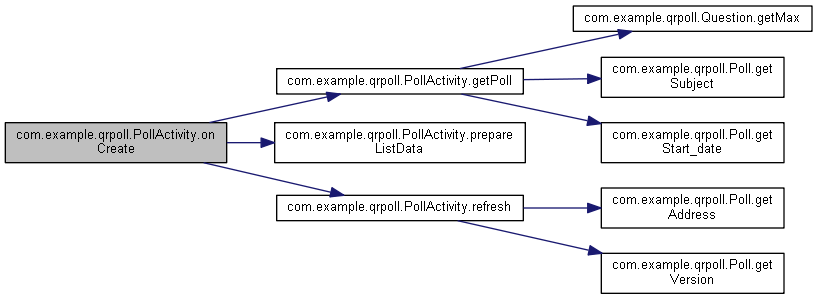
\includegraphics[width=350pt]{classcom_1_1example_1_1qrpoll_1_1_poll_activity_a9982a68e4862d0e8793e0a2e88373589_cgraph}
\end{center}
\end{figure}


\hypertarget{classcom_1_1example_1_1qrpoll_1_1_poll_activity_a288dc770b6c610732839043961870030}{\index{com\+::example\+::qrpoll\+::\+Poll\+Activity@{com\+::example\+::qrpoll\+::\+Poll\+Activity}!on\+Create\+Options\+Menu@{on\+Create\+Options\+Menu}}
\index{on\+Create\+Options\+Menu@{on\+Create\+Options\+Menu}!com\+::example\+::qrpoll\+::\+Poll\+Activity@{com\+::example\+::qrpoll\+::\+Poll\+Activity}}
\subsubsection[{on\+Create\+Options\+Menu}]{\setlength{\rightskip}{0pt plus 5cm}boolean com.\+example.\+qrpoll.\+Poll\+Activity.\+on\+Create\+Options\+Menu (
\begin{DoxyParamCaption}
\item[{Menu}]{menu}
\end{DoxyParamCaption}
)}}\label{classcom_1_1example_1_1qrpoll_1_1_poll_activity_a288dc770b6c610732839043961870030}
tworzenie menu 

Definicja w linii 78 pliku Poll\+Activity.\+java.


\begin{DoxyCode}
78                                                   \{
79         MenuInflater menuInflater = getMenuInflater();
80         menuInflater.inflate(R.layout.menu, menu);
81         \textcolor{keywordflow}{return} \textcolor{keyword}{true};
82     \}
\end{DoxyCode}
\hypertarget{classcom_1_1example_1_1qrpoll_1_1_poll_activity_afc58ce75d02a97bc6e93085c1c23281a}{\index{com\+::example\+::qrpoll\+::\+Poll\+Activity@{com\+::example\+::qrpoll\+::\+Poll\+Activity}!on\+Options\+Item\+Selected@{on\+Options\+Item\+Selected}}
\index{on\+Options\+Item\+Selected@{on\+Options\+Item\+Selected}!com\+::example\+::qrpoll\+::\+Poll\+Activity@{com\+::example\+::qrpoll\+::\+Poll\+Activity}}
\subsubsection[{on\+Options\+Item\+Selected}]{\setlength{\rightskip}{0pt plus 5cm}boolean com.\+example.\+qrpoll.\+Poll\+Activity.\+on\+Options\+Item\+Selected (
\begin{DoxyParamCaption}
\item[{Menu\+Item}]{item}
\end{DoxyParamCaption}
)}}\label{classcom_1_1example_1_1qrpoll_1_1_poll_activity_afc58ce75d02a97bc6e93085c1c23281a}
reagowanie na klikniecie na przyciski w menu 

Definicja w linii 88 pliku Poll\+Activity.\+java.


\begin{DoxyCode}
88                                                         \{
89         \textcolor{keywordtype}{int} \textcolor{keywordtype}{id} = item.getItemId();
90         \textcolor{keywordflow}{if} (\textcolor{keywordtype}{id} == R.id.historia) \{
91             Intent it=\textcolor{keyword}{new} Intent(getApplication(),HistoryLayout.class);
92             startActivity(it);
93             
94             \textcolor{keywordflow}{return} \textcolor{keyword}{true};
95         \}\textcolor{keywordflow}{else} \textcolor{keywordflow}{if}(\textcolor{keywordtype}{id}==R.id.odswiez)\{
96             
97             \hyperlink{classcom_1_1example_1_1qrpoll_1_1_poll_activity_a6c59d6b3beb1d5fea9899b0b0cb51e1f}{refresh}();
98         \}
99         \textcolor{keywordflow}{return} super.onOptionsItemSelected(item);
100     \}
\end{DoxyCode}


Oto graf wywołań dla tej funkcji\+:
\nopagebreak
\begin{figure}[H]
\begin{center}
\leavevmode
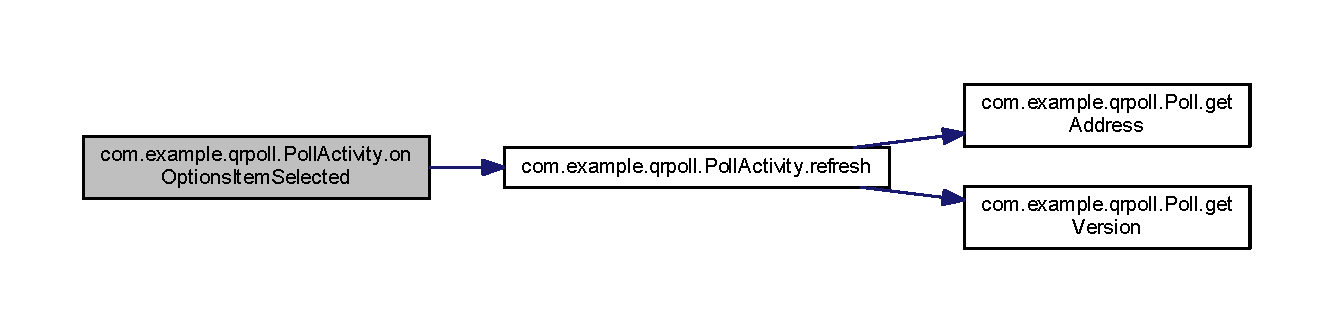
\includegraphics[width=350pt]{classcom_1_1example_1_1qrpoll_1_1_poll_activity_afc58ce75d02a97bc6e93085c1c23281a_cgraph}
\end{center}
\end{figure}


\hypertarget{classcom_1_1example_1_1qrpoll_1_1_poll_activity_a1081f69211873eaf38c422ea12c769f0}{\index{com\+::example\+::qrpoll\+::\+Poll\+Activity@{com\+::example\+::qrpoll\+::\+Poll\+Activity}!prepare\+List\+Data@{prepare\+List\+Data}}
\index{prepare\+List\+Data@{prepare\+List\+Data}!com\+::example\+::qrpoll\+::\+Poll\+Activity@{com\+::example\+::qrpoll\+::\+Poll\+Activity}}
\subsubsection[{prepare\+List\+Data}]{\setlength{\rightskip}{0pt plus 5cm}void com.\+example.\+qrpoll.\+Poll\+Activity.\+prepare\+List\+Data (
\begin{DoxyParamCaption}
{}
\end{DoxyParamCaption}
)\hspace{0.3cm}{\ttfamily [private]}}}\label{classcom_1_1example_1_1qrpoll_1_1_poll_activity_a1081f69211873eaf38c422ea12c769f0}
Przygotowanie naglowkow rozsuwanej listy do wyswietlenia 

Definicja w linii 60 pliku Poll\+Activity.\+java.


\begin{DoxyCode}
60                                    \{
61         \hyperlink{classcom_1_1example_1_1qrpoll_1_1_poll_activity_a62dde3c117f038e463aa7174906f5f7b}{listDataHeader} = \textcolor{keyword}{new} ArrayList<String>();
62         \hyperlink{classcom_1_1example_1_1qrpoll_1_1_poll_activity_ab607bec81e729232d72cee9db8ffdc73}{listDataChild} = \textcolor{keyword}{new} HashMap<String, List<String>>();
63         \hyperlink{classcom_1_1example_1_1qrpoll_1_1_poll_activity_a62dde3c117f038e463aa7174906f5f7b}{listDataHeader}=\hyperlink{classcom_1_1example_1_1qrpoll_1_1_poll_activity_ae9caea6dcd77802d9edc7f86ace0fc5c}{questions};
64         
65         \textcolor{keywordflow}{for}(\textcolor{keywordtype}{int} i =0;i<listDataHeader.size();i++)\{
66             List<String> list = \textcolor{keyword}{new} ArrayList<String>();
67             list.add(\textcolor{stringliteral}{""});
68             listDataChild.put(listDataHeader.get(i),list);
69         \}
70 
71     \}
\end{DoxyCode}


Oto graf wywoływań tej funkcji\+:
\nopagebreak
\begin{figure}[H]
\begin{center}
\leavevmode
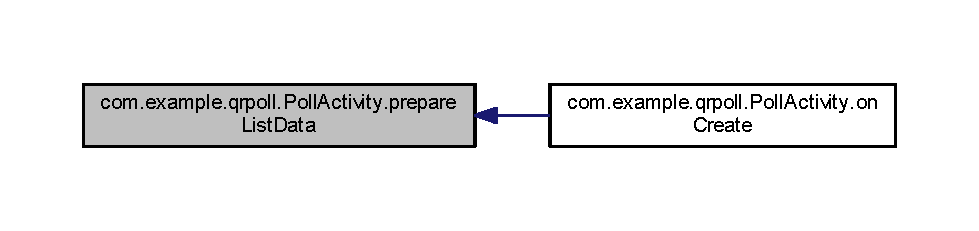
\includegraphics[width=350pt]{classcom_1_1example_1_1qrpoll_1_1_poll_activity_a1081f69211873eaf38c422ea12c769f0_icgraph}
\end{center}
\end{figure}


\hypertarget{classcom_1_1example_1_1qrpoll_1_1_poll_activity_a6c59d6b3beb1d5fea9899b0b0cb51e1f}{\index{com\+::example\+::qrpoll\+::\+Poll\+Activity@{com\+::example\+::qrpoll\+::\+Poll\+Activity}!refresh@{refresh}}
\index{refresh@{refresh}!com\+::example\+::qrpoll\+::\+Poll\+Activity@{com\+::example\+::qrpoll\+::\+Poll\+Activity}}
\subsubsection[{refresh}]{\setlength{\rightskip}{0pt plus 5cm}void com.\+example.\+qrpoll.\+Poll\+Activity.\+refresh (
\begin{DoxyParamCaption}
{}
\end{DoxyParamCaption}
)}}\label{classcom_1_1example_1_1qrpoll_1_1_poll_activity_a6c59d6b3beb1d5fea9899b0b0cb51e1f}
metoda wywolywana przez klikniecie \char`\"{}odswiez\char`\"{}, sprawdzajaca czy na serwerze nie pojawila sie nowa wersja ankiety 

Definicja w linii 280 pliku Poll\+Activity.\+java.


\begin{DoxyCode}
280                          \{
281         \textcolor{keywordflow}{try} \{
282             Poll p=\textcolor{keyword}{new} Poll(\hyperlink{classcom_1_1example_1_1qrpoll_1_1_poll_activity_accbd807fe57852d64377c5a96401c376}{poll}.\hyperlink{classcom_1_1example_1_1qrpoll_1_1_poll_ac84c3d1747b6eb8d4f43da448de8080f}{getAddress}(),getApplicationContext());
283             \textcolor{keywordflow}{if}(\hyperlink{classcom_1_1example_1_1qrpoll_1_1_poll_activity_accbd807fe57852d64377c5a96401c376}{poll}.\hyperlink{classcom_1_1example_1_1qrpoll_1_1_poll_a6ec1751ddf25a1b00173e1c4f3203458}{getVersion}()!=p.getVersion())\{
284                 Intent it=\textcolor{keyword}{new} Intent(getApplication(),PollActivity.class);
285                 it.putExtra(\textcolor{stringliteral}{"scanResult"}, poll.getAddress().substring(7));
286                 it.putExtra(\textcolor{stringliteral}{"message"}, \textcolor{stringliteral}{"nowa wersja"});
287                 startActivity(it);
288                 finish();
289             \}\textcolor{keywordflow}{else}\{
290                 Toast.makeText(getApplicationContext(),
291                        \textcolor{stringliteral}{"Nie ma nowszej wersji"}, Toast.LENGTH\_SHORT).show();
292             \}
293         \} \textcolor{keywordflow}{catch} (JSONException e) \{
294             \textcolor{comment}{// TODO Auto-generated catch block}
295             e.printStackTrace();
296         \}\textcolor{keywordflow}{catch}(NullPointerException e)\{
297             Toast.makeText(getApplicationContext(),
298                        \textcolor{stringliteral}{"Brak polaczenia"}, Toast.LENGTH\_SHORT).show();
299         \}
300     \}
\end{DoxyCode}


Oto graf wywołań dla tej funkcji\+:
\nopagebreak
\begin{figure}[H]
\begin{center}
\leavevmode
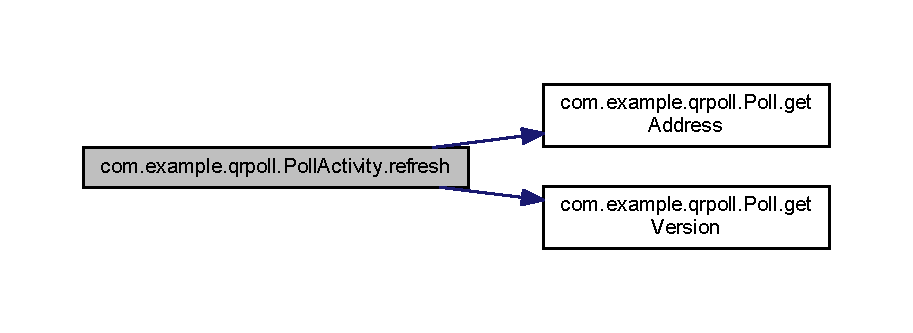
\includegraphics[width=350pt]{classcom_1_1example_1_1qrpoll_1_1_poll_activity_a6c59d6b3beb1d5fea9899b0b0cb51e1f_cgraph}
\end{center}
\end{figure}




Oto graf wywoływań tej funkcji\+:
\nopagebreak
\begin{figure}[H]
\begin{center}
\leavevmode
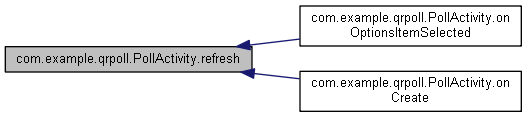
\includegraphics[width=350pt]{classcom_1_1example_1_1qrpoll_1_1_poll_activity_a6c59d6b3beb1d5fea9899b0b0cb51e1f_icgraph}
\end{center}
\end{figure}




\subsection{Dokumentacja atrybutów składowych}
\hypertarget{classcom_1_1example_1_1qrpoll_1_1_poll_activity_a0cb80128cd6ae3abb14437dbcf82f876}{\index{com\+::example\+::qrpoll\+::\+Poll\+Activity@{com\+::example\+::qrpoll\+::\+Poll\+Activity}!back\+Button\+Count@{back\+Button\+Count}}
\index{back\+Button\+Count@{back\+Button\+Count}!com\+::example\+::qrpoll\+::\+Poll\+Activity@{com\+::example\+::qrpoll\+::\+Poll\+Activity}}
\subsubsection[{back\+Button\+Count}]{\setlength{\rightskip}{0pt plus 5cm}int com.\+example.\+qrpoll.\+Poll\+Activity.\+back\+Button\+Count =0\hspace{0.3cm}{\ttfamily [private]}}}\label{classcom_1_1example_1_1qrpoll_1_1_poll_activity_a0cb80128cd6ae3abb14437dbcf82f876}


Definicja w linii 52 pliku Poll\+Activity.\+java.

\hypertarget{classcom_1_1example_1_1qrpoll_1_1_poll_activity_a45d9887fce62772f80726024d1775f7d}{\index{com\+::example\+::qrpoll\+::\+Poll\+Activity@{com\+::example\+::qrpoll\+::\+Poll\+Activity}!exp\+List\+View@{exp\+List\+View}}
\index{exp\+List\+View@{exp\+List\+View}!com\+::example\+::qrpoll\+::\+Poll\+Activity@{com\+::example\+::qrpoll\+::\+Poll\+Activity}}
\subsubsection[{exp\+List\+View}]{\setlength{\rightskip}{0pt plus 5cm}Expandable\+List\+View com.\+example.\+qrpoll.\+Poll\+Activity.\+exp\+List\+View\hspace{0.3cm}{\ttfamily [package]}}}\label{classcom_1_1example_1_1qrpoll_1_1_poll_activity_a45d9887fce62772f80726024d1775f7d}


Definicja w linii 42 pliku Poll\+Activity.\+java.

\hypertarget{classcom_1_1example_1_1qrpoll_1_1_poll_activity_aeedb4d35f1bb56db80b834a5c5da4f44}{\index{com\+::example\+::qrpoll\+::\+Poll\+Activity@{com\+::example\+::qrpoll\+::\+Poll\+Activity}!list\+Adapter@{list\+Adapter}}
\index{list\+Adapter@{list\+Adapter}!com\+::example\+::qrpoll\+::\+Poll\+Activity@{com\+::example\+::qrpoll\+::\+Poll\+Activity}}
\subsubsection[{list\+Adapter}]{\setlength{\rightskip}{0pt plus 5cm}{\bf Expandable\+List\+Adapter} com.\+example.\+qrpoll.\+Poll\+Activity.\+list\+Adapter\hspace{0.3cm}{\ttfamily [package]}}}\label{classcom_1_1example_1_1qrpoll_1_1_poll_activity_aeedb4d35f1bb56db80b834a5c5da4f44}


Definicja w linii 41 pliku Poll\+Activity.\+java.

\hypertarget{classcom_1_1example_1_1qrpoll_1_1_poll_activity_ab607bec81e729232d72cee9db8ffdc73}{\index{com\+::example\+::qrpoll\+::\+Poll\+Activity@{com\+::example\+::qrpoll\+::\+Poll\+Activity}!list\+Data\+Child@{list\+Data\+Child}}
\index{list\+Data\+Child@{list\+Data\+Child}!com\+::example\+::qrpoll\+::\+Poll\+Activity@{com\+::example\+::qrpoll\+::\+Poll\+Activity}}
\subsubsection[{list\+Data\+Child}]{\setlength{\rightskip}{0pt plus 5cm}Hash\+Map$<$String, List$<$String$>$ $>$ com.\+example.\+qrpoll.\+Poll\+Activity.\+list\+Data\+Child\hspace{0.3cm}{\ttfamily [package]}}}\label{classcom_1_1example_1_1qrpoll_1_1_poll_activity_ab607bec81e729232d72cee9db8ffdc73}


Definicja w linii 44 pliku Poll\+Activity.\+java.

\hypertarget{classcom_1_1example_1_1qrpoll_1_1_poll_activity_a62dde3c117f038e463aa7174906f5f7b}{\index{com\+::example\+::qrpoll\+::\+Poll\+Activity@{com\+::example\+::qrpoll\+::\+Poll\+Activity}!list\+Data\+Header@{list\+Data\+Header}}
\index{list\+Data\+Header@{list\+Data\+Header}!com\+::example\+::qrpoll\+::\+Poll\+Activity@{com\+::example\+::qrpoll\+::\+Poll\+Activity}}
\subsubsection[{list\+Data\+Header}]{\setlength{\rightskip}{0pt plus 5cm}List$<$String$>$ com.\+example.\+qrpoll.\+Poll\+Activity.\+list\+Data\+Header\hspace{0.3cm}{\ttfamily [package]}}}\label{classcom_1_1example_1_1qrpoll_1_1_poll_activity_a62dde3c117f038e463aa7174906f5f7b}


Definicja w linii 43 pliku Poll\+Activity.\+java.

\hypertarget{classcom_1_1example_1_1qrpoll_1_1_poll_activity_accbd807fe57852d64377c5a96401c376}{\index{com\+::example\+::qrpoll\+::\+Poll\+Activity@{com\+::example\+::qrpoll\+::\+Poll\+Activity}!poll@{poll}}
\index{poll@{poll}!com\+::example\+::qrpoll\+::\+Poll\+Activity@{com\+::example\+::qrpoll\+::\+Poll\+Activity}}
\subsubsection[{poll}]{\setlength{\rightskip}{0pt plus 5cm}{\bf Poll} com.\+example.\+qrpoll.\+Poll\+Activity.\+poll = null\hspace{0.3cm}{\ttfamily [private]}}}\label{classcom_1_1example_1_1qrpoll_1_1_poll_activity_accbd807fe57852d64377c5a96401c376}


Definicja w linii 56 pliku Poll\+Activity.\+java.

\hypertarget{classcom_1_1example_1_1qrpoll_1_1_poll_activity_ae9caea6dcd77802d9edc7f86ace0fc5c}{\index{com\+::example\+::qrpoll\+::\+Poll\+Activity@{com\+::example\+::qrpoll\+::\+Poll\+Activity}!questions@{questions}}
\index{questions@{questions}!com\+::example\+::qrpoll\+::\+Poll\+Activity@{com\+::example\+::qrpoll\+::\+Poll\+Activity}}
\subsubsection[{questions}]{\setlength{\rightskip}{0pt plus 5cm}List$<$String$>$ com.\+example.\+qrpoll.\+Poll\+Activity.\+questions\hspace{0.3cm}{\ttfamily [private]}}}\label{classcom_1_1example_1_1qrpoll_1_1_poll_activity_ae9caea6dcd77802d9edc7f86ace0fc5c}


Definicja w linii 46 pliku Poll\+Activity.\+java.

\hypertarget{classcom_1_1example_1_1qrpoll_1_1_poll_activity_a3c2b3e0864209b0253263a7af2642a13}{\index{com\+::example\+::qrpoll\+::\+Poll\+Activity@{com\+::example\+::qrpoll\+::\+Poll\+Activity}!rb@{rb}}
\index{rb@{rb}!com\+::example\+::qrpoll\+::\+Poll\+Activity@{com\+::example\+::qrpoll\+::\+Poll\+Activity}}
\subsubsection[{rb}]{\setlength{\rightskip}{0pt plus 5cm}Rating\+Bar com.\+example.\+qrpoll.\+Poll\+Activity.\+rb\hspace{0.3cm}{\ttfamily [private]}}}\label{classcom_1_1example_1_1qrpoll_1_1_poll_activity_a3c2b3e0864209b0253263a7af2642a13}


Definicja w linii 53 pliku Poll\+Activity.\+java.

\hypertarget{classcom_1_1example_1_1qrpoll_1_1_poll_activity_a7928323c2d0f40aa25420488718de309}{\index{com\+::example\+::qrpoll\+::\+Poll\+Activity@{com\+::example\+::qrpoll\+::\+Poll\+Activity}!tv1@{tv1}}
\index{tv1@{tv1}!com\+::example\+::qrpoll\+::\+Poll\+Activity@{com\+::example\+::qrpoll\+::\+Poll\+Activity}}
\subsubsection[{tv1}]{\setlength{\rightskip}{0pt plus 5cm}Text\+View com.\+example.\+qrpoll.\+Poll\+Activity.\+tv1\hspace{0.3cm}{\ttfamily [private]}}}\label{classcom_1_1example_1_1qrpoll_1_1_poll_activity_a7928323c2d0f40aa25420488718de309}


Definicja w linii 47 pliku Poll\+Activity.\+java.

\hypertarget{classcom_1_1example_1_1qrpoll_1_1_poll_activity_a48f7da0dc1da430cd5ac90a8376cad70}{\index{com\+::example\+::qrpoll\+::\+Poll\+Activity@{com\+::example\+::qrpoll\+::\+Poll\+Activity}!tv2@{tv2}}
\index{tv2@{tv2}!com\+::example\+::qrpoll\+::\+Poll\+Activity@{com\+::example\+::qrpoll\+::\+Poll\+Activity}}
\subsubsection[{tv2}]{\setlength{\rightskip}{0pt plus 5cm}Text\+View com.\+example.\+qrpoll.\+Poll\+Activity.\+tv2\hspace{0.3cm}{\ttfamily [private]}}}\label{classcom_1_1example_1_1qrpoll_1_1_poll_activity_a48f7da0dc1da430cd5ac90a8376cad70}


Definicja w linii 48 pliku Poll\+Activity.\+java.

\hypertarget{classcom_1_1example_1_1qrpoll_1_1_poll_activity_a70708751ea7eb8a32569447a087471b8}{\index{com\+::example\+::qrpoll\+::\+Poll\+Activity@{com\+::example\+::qrpoll\+::\+Poll\+Activity}!tv3@{tv3}}
\index{tv3@{tv3}!com\+::example\+::qrpoll\+::\+Poll\+Activity@{com\+::example\+::qrpoll\+::\+Poll\+Activity}}
\subsubsection[{tv3}]{\setlength{\rightskip}{0pt plus 5cm}Text\+View com.\+example.\+qrpoll.\+Poll\+Activity.\+tv3\hspace{0.3cm}{\ttfamily [private]}}}\label{classcom_1_1example_1_1qrpoll_1_1_poll_activity_a70708751ea7eb8a32569447a087471b8}


Definicja w linii 49 pliku Poll\+Activity.\+java.

\hypertarget{classcom_1_1example_1_1qrpoll_1_1_poll_activity_a32c7797e7d6cdf269f9449cfdb635438}{\index{com\+::example\+::qrpoll\+::\+Poll\+Activity@{com\+::example\+::qrpoll\+::\+Poll\+Activity}!tv4@{tv4}}
\index{tv4@{tv4}!com\+::example\+::qrpoll\+::\+Poll\+Activity@{com\+::example\+::qrpoll\+::\+Poll\+Activity}}
\subsubsection[{tv4}]{\setlength{\rightskip}{0pt plus 5cm}Text\+View com.\+example.\+qrpoll.\+Poll\+Activity.\+tv4\hspace{0.3cm}{\ttfamily [private]}}}\label{classcom_1_1example_1_1qrpoll_1_1_poll_activity_a32c7797e7d6cdf269f9449cfdb635438}


Definicja w linii 50 pliku Poll\+Activity.\+java.

\hypertarget{classcom_1_1example_1_1qrpoll_1_1_poll_activity_a4fbbfc95809c5aa0bf9916316730a992}{\index{com\+::example\+::qrpoll\+::\+Poll\+Activity@{com\+::example\+::qrpoll\+::\+Poll\+Activity}!version@{version}}
\index{version@{version}!com\+::example\+::qrpoll\+::\+Poll\+Activity@{com\+::example\+::qrpoll\+::\+Poll\+Activity}}
\subsubsection[{version}]{\setlength{\rightskip}{0pt plus 5cm}Text\+View com.\+example.\+qrpoll.\+Poll\+Activity.\+version\hspace{0.3cm}{\ttfamily [private]}}}\label{classcom_1_1example_1_1qrpoll_1_1_poll_activity_a4fbbfc95809c5aa0bf9916316730a992}


Definicja w linii 51 pliku Poll\+Activity.\+java.



Dokumentacja dla tej klasy została wygenerowana z pliku\+:\begin{DoxyCompactItemize}
\item 
C\+:/\+Users/\+Wodzu/\+Documents/\+Git\+Hub/\+Projekt\+Zespolowy/\+Android Final + dokumentacja/android/qrpoll/src/com/example/qrpoll/\hyperlink{_poll_activity_8java}{Poll\+Activity.\+java}\end{DoxyCompactItemize}

\hypertarget{classcom_1_1example_1_1qrpoll_1_1_question}{\section{Dokumentacja klasy com.\+example.\+qrpoll.\+Question}
\label{classcom_1_1example_1_1qrpoll_1_1_question}\index{com.\+example.\+qrpoll.\+Question@{com.\+example.\+qrpoll.\+Question}}
}


Diagram współpracy dla com.\+example.\+qrpoll.\+Question\+:\nopagebreak
\begin{figure}[H]
\begin{center}
\leavevmode
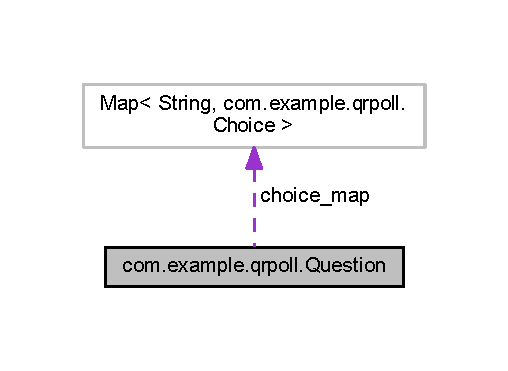
\includegraphics[width=244pt]{classcom_1_1example_1_1qrpoll_1_1_question__coll__graph}
\end{center}
\end{figure}
\subsection*{Metody publiczne}
\begin{DoxyCompactItemize}
\item 
void \hyperlink{classcom_1_1example_1_1qrpoll_1_1_question_ab9e20bf997816ae32b9e3312f48d124f}{add\+Choice} (String \hyperlink{classcom_1_1example_1_1qrpoll_1_1_question_ab94e31e243d24239faf4ae4c68c28f0b}{pk}, String choice\+\_\+text)
\item 
String \hyperlink{classcom_1_1example_1_1qrpoll_1_1_question_a7b4c664c6c4ebec154ea7132c75bc88d}{get\+Pk} ()
\item 
String \hyperlink{classcom_1_1example_1_1qrpoll_1_1_question_a06182185a203fccb72e4421a10a8a511}{get\+Max} ()
\item 
String \hyperlink{classcom_1_1example_1_1qrpoll_1_1_question_ac79778f9afb3c040d0c6f4ada39fb34a}{get\+Question\+\_\+text} ()
\item 
Map$<$ String, \hyperlink{classcom_1_1example_1_1qrpoll_1_1_choice}{Choice} $>$ \hyperlink{classcom_1_1example_1_1qrpoll_1_1_question_a7ec19ad963a2fcaa76c29feb59129702}{get\+Choice\+\_\+map} ()
\item 
String \hyperlink{classcom_1_1example_1_1qrpoll_1_1_question_aa5e300a74cf22554ee7221da00aff666}{is\+Rating} ()
\item 
int \hyperlink{classcom_1_1example_1_1qrpoll_1_1_question_a3608f9d26af608c85ac88ee48e68f624}{hash\+Code} ()
\item 
boolean \hyperlink{classcom_1_1example_1_1qrpoll_1_1_question_a9aa72d6cf0140674837bd6f2399631ed}{equals} (Object obj)
\end{DoxyCompactItemize}
\subsection*{Funkcje pakietu}
\begin{DoxyCompactItemize}
\item 
\hyperlink{classcom_1_1example_1_1qrpoll_1_1_question_aeeae84aca53cbbce8820daf91436564c}{Question} (String \hyperlink{classcom_1_1example_1_1qrpoll_1_1_question_ab94e31e243d24239faf4ae4c68c28f0b}{pk}, String \hyperlink{classcom_1_1example_1_1qrpoll_1_1_question_ab90d61211a23303be8fe8139aed31754}{question\+\_\+text}, String \hyperlink{classcom_1_1example_1_1qrpoll_1_1_question_a7b9016a004baf976a3d700ce332c0e1b}{is\+Rating}, String \hyperlink{classcom_1_1example_1_1qrpoll_1_1_question_a07bd283882253cc7c9ab69718a692a64}{max})
\end{DoxyCompactItemize}
\subsection*{Atrybuty prywatne}
\begin{DoxyCompactItemize}
\item 
String \hyperlink{classcom_1_1example_1_1qrpoll_1_1_question_ab94e31e243d24239faf4ae4c68c28f0b}{pk}
\item 
String \hyperlink{classcom_1_1example_1_1qrpoll_1_1_question_ab90d61211a23303be8fe8139aed31754}{question\+\_\+text}
\item 
String \hyperlink{classcom_1_1example_1_1qrpoll_1_1_question_a7b9016a004baf976a3d700ce332c0e1b}{is\+Rating}
\item 
String \hyperlink{classcom_1_1example_1_1qrpoll_1_1_question_a07bd283882253cc7c9ab69718a692a64}{max}
\item 
Map$<$ String, \hyperlink{classcom_1_1example_1_1qrpoll_1_1_choice}{Choice} $>$ \hyperlink{classcom_1_1example_1_1qrpoll_1_1_question_aa382153815db46e065ab637ef86f9265}{choice\+\_\+map}
\end{DoxyCompactItemize}


\subsection{Opis szczegółowy}
\begin{DoxyAuthor}{Autor}
Piotrek 

Sliwka klasa reprezentujaca pojedyńcze pytanie wchodzace w sklad ankiety, posiada mape odpowiedzi 
\end{DoxyAuthor}


Definicja w linii 21 pliku Question.\+java.



\subsection{Dokumentacja konstruktora i destruktora}
\hypertarget{classcom_1_1example_1_1qrpoll_1_1_question_aeeae84aca53cbbce8820daf91436564c}{\index{com\+::example\+::qrpoll\+::\+Question@{com\+::example\+::qrpoll\+::\+Question}!Question@{Question}}
\index{Question@{Question}!com\+::example\+::qrpoll\+::\+Question@{com\+::example\+::qrpoll\+::\+Question}}
\subsubsection[{Question}]{\setlength{\rightskip}{0pt plus 5cm}com.\+example.\+qrpoll.\+Question.\+Question (
\begin{DoxyParamCaption}
\item[{String}]{pk, }
\item[{String}]{question\+\_\+text, }
\item[{String}]{is\+Rating, }
\item[{String}]{max}
\end{DoxyParamCaption}
)\hspace{0.3cm}{\ttfamily [package]}}}\label{classcom_1_1example_1_1qrpoll_1_1_question_aeeae84aca53cbbce8820daf91436564c}
glowny konstruktor 
\begin{DoxyParams}{Parametry}
{\em pk} & id pytania \\
\hline
{\em question\+\_\+text} & \\
\hline
{\em is\+Rating} & zmienna, ktora okresla czy pytanie ma byc wyswietlone czy nie \\
\hline
{\em max} & maksymalna ilosc odpowiedzi na dane pytanie \\
\hline
\end{DoxyParams}


Definicja w linii 35 pliku Question.\+java.


\begin{DoxyCode}
35                                                                         \{
36         this.pk = \hyperlink{classcom_1_1example_1_1qrpoll_1_1_question_ab94e31e243d24239faf4ae4c68c28f0b}{pk};
37         this.question\_text = \hyperlink{classcom_1_1example_1_1qrpoll_1_1_question_ab90d61211a23303be8fe8139aed31754}{question\_text};
38         this.isRating=\hyperlink{classcom_1_1example_1_1qrpoll_1_1_question_aa5e300a74cf22554ee7221da00aff666}{isRating};
39         this.max=\hyperlink{classcom_1_1example_1_1qrpoll_1_1_question_a07bd283882253cc7c9ab69718a692a64}{max};
40         this.choice\_map = \textcolor{keyword}{new} HashMap<String,Choice>(); \textcolor{comment}{//Map<PK,Choice>}
41     \}
\end{DoxyCode}


Oto graf wywołań dla tej funkcji\+:
\nopagebreak
\begin{figure}[H]
\begin{center}
\leavevmode
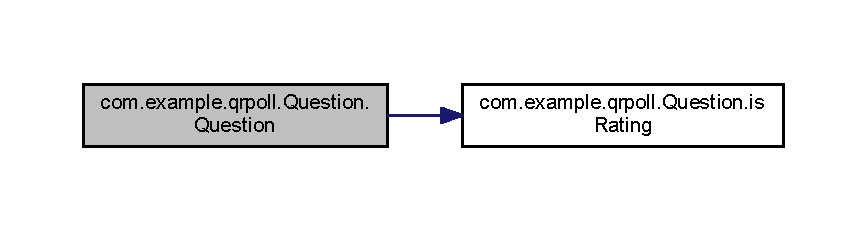
\includegraphics[width=350pt]{classcom_1_1example_1_1qrpoll_1_1_question_aeeae84aca53cbbce8820daf91436564c_cgraph}
\end{center}
\end{figure}




Oto graf wywoływań tej funkcji\+:
\nopagebreak
\begin{figure}[H]
\begin{center}
\leavevmode
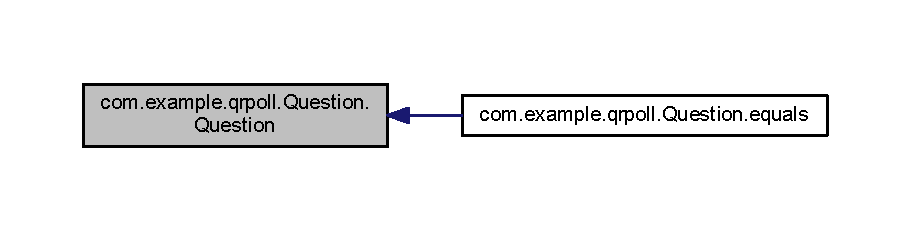
\includegraphics[width=350pt]{classcom_1_1example_1_1qrpoll_1_1_question_aeeae84aca53cbbce8820daf91436564c_icgraph}
\end{center}
\end{figure}




\subsection{Dokumentacja funkcji składowych}
\hypertarget{classcom_1_1example_1_1qrpoll_1_1_question_ab9e20bf997816ae32b9e3312f48d124f}{\index{com\+::example\+::qrpoll\+::\+Question@{com\+::example\+::qrpoll\+::\+Question}!add\+Choice@{add\+Choice}}
\index{add\+Choice@{add\+Choice}!com\+::example\+::qrpoll\+::\+Question@{com\+::example\+::qrpoll\+::\+Question}}
\subsubsection[{add\+Choice}]{\setlength{\rightskip}{0pt plus 5cm}void com.\+example.\+qrpoll.\+Question.\+add\+Choice (
\begin{DoxyParamCaption}
\item[{String}]{pk, }
\item[{String}]{choice\+\_\+text}
\end{DoxyParamCaption}
)}}\label{classcom_1_1example_1_1qrpoll_1_1_question_ab9e20bf997816ae32b9e3312f48d124f}
dodaje odpowiedz o danej tresci i id do pytania 
\begin{DoxyParams}{Parametry}
{\em pk} & id pytania \\
\hline
{\em choice\+\_\+text} & tresc odpowiedzi \\
\hline
\end{DoxyParams}


Definicja w linii 48 pliku Question.\+java.


\begin{DoxyCode}
48                                                         \{
49         choice\_map.put(\hyperlink{classcom_1_1example_1_1qrpoll_1_1_question_ab94e31e243d24239faf4ae4c68c28f0b}{pk},(\textcolor{keyword}{new} Choice(pk, choice\_text)));
50     \}
\end{DoxyCode}
\hypertarget{classcom_1_1example_1_1qrpoll_1_1_question_a9aa72d6cf0140674837bd6f2399631ed}{\index{com\+::example\+::qrpoll\+::\+Question@{com\+::example\+::qrpoll\+::\+Question}!equals@{equals}}
\index{equals@{equals}!com\+::example\+::qrpoll\+::\+Question@{com\+::example\+::qrpoll\+::\+Question}}
\subsubsection[{equals}]{\setlength{\rightskip}{0pt plus 5cm}boolean com.\+example.\+qrpoll.\+Question.\+equals (
\begin{DoxyParamCaption}
\item[{Object}]{obj}
\end{DoxyParamCaption}
)}}\label{classcom_1_1example_1_1qrpoll_1_1_question_a9aa72d6cf0140674837bd6f2399631ed}
porownuje dwa obiekty klasy \hyperlink{classcom_1_1example_1_1qrpoll_1_1_question}{Question} 
\begin{DoxyParams}{Parametry}
{\em obj} & \\
\hline
\end{DoxyParams}
\begin{DoxyReturn}{Zwraca}

\end{DoxyReturn}


Definicja w linii 107 pliku Question.\+java.


\begin{DoxyCode}
107                                       \{
108         \textcolor{keywordflow}{if} (\textcolor{keyword}{this} == obj)
109             \textcolor{keywordflow}{return} \textcolor{keyword}{true};
110         \textcolor{keywordflow}{if} (obj == null)
111             \textcolor{keywordflow}{return} \textcolor{keyword}{false};
112         \textcolor{keywordflow}{if} (getClass() != obj.getClass())
113             \textcolor{keywordflow}{return} \textcolor{keyword}{false};
114         \hyperlink{classcom_1_1example_1_1qrpoll_1_1_question_aeeae84aca53cbbce8820daf91436564c}{Question} other = (\hyperlink{classcom_1_1example_1_1qrpoll_1_1_question_aeeae84aca53cbbce8820daf91436564c}{Question}) obj;
115         \textcolor{keywordflow}{if} (\hyperlink{classcom_1_1example_1_1qrpoll_1_1_question_aa382153815db46e065ab637ef86f9265}{choice\_map} == null) \{
116             \textcolor{keywordflow}{if} (other.choice\_map != null)
117                 \textcolor{keywordflow}{return} \textcolor{keyword}{false};
118         \} \textcolor{keywordflow}{else} \textcolor{keywordflow}{if} (!\hyperlink{classcom_1_1example_1_1qrpoll_1_1_question_aa382153815db46e065ab637ef86f9265}{choice\_map}.equals(other.choice\_map))
119             \textcolor{keywordflow}{return} \textcolor{keyword}{false};
120         \textcolor{keywordflow}{if} (\hyperlink{classcom_1_1example_1_1qrpoll_1_1_question_ab94e31e243d24239faf4ae4c68c28f0b}{pk} == null) \{
121             \textcolor{keywordflow}{if} (other.pk != null)
122                 \textcolor{keywordflow}{return} \textcolor{keyword}{false};
123         \} \textcolor{keywordflow}{else} \textcolor{keywordflow}{if} (!\hyperlink{classcom_1_1example_1_1qrpoll_1_1_question_ab94e31e243d24239faf4ae4c68c28f0b}{pk}.equals(other.pk))
124             \textcolor{keywordflow}{return} \textcolor{keyword}{false};
125         \textcolor{keywordflow}{if} (\hyperlink{classcom_1_1example_1_1qrpoll_1_1_question_ab90d61211a23303be8fe8139aed31754}{question\_text} == null) \{
126             \textcolor{keywordflow}{if} (other.question\_text != null)
127                 \textcolor{keywordflow}{return} \textcolor{keyword}{false};
128         \} \textcolor{keywordflow}{else} \textcolor{keywordflow}{if} (!\hyperlink{classcom_1_1example_1_1qrpoll_1_1_question_ab90d61211a23303be8fe8139aed31754}{question\_text}.equals(other.question\_text))
129             \textcolor{keywordflow}{return} \textcolor{keyword}{false};
130         \textcolor{keywordflow}{return} \textcolor{keyword}{true};
131     \}
\end{DoxyCode}


Oto graf wywołań dla tej funkcji\+:
\nopagebreak
\begin{figure}[H]
\begin{center}
\leavevmode
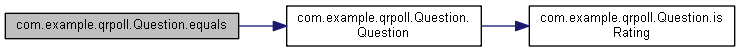
\includegraphics[width=350pt]{classcom_1_1example_1_1qrpoll_1_1_question_a9aa72d6cf0140674837bd6f2399631ed_cgraph}
\end{center}
\end{figure}


\hypertarget{classcom_1_1example_1_1qrpoll_1_1_question_a7ec19ad963a2fcaa76c29feb59129702}{\index{com\+::example\+::qrpoll\+::\+Question@{com\+::example\+::qrpoll\+::\+Question}!get\+Choice\+\_\+map@{get\+Choice\+\_\+map}}
\index{get\+Choice\+\_\+map@{get\+Choice\+\_\+map}!com\+::example\+::qrpoll\+::\+Question@{com\+::example\+::qrpoll\+::\+Question}}
\subsubsection[{get\+Choice\+\_\+map}]{\setlength{\rightskip}{0pt plus 5cm}Map$<$String, {\bf Choice}$>$ com.\+example.\+qrpoll.\+Question.\+get\+Choice\+\_\+map (
\begin{DoxyParamCaption}
{}
\end{DoxyParamCaption}
)}}\label{classcom_1_1example_1_1qrpoll_1_1_question_a7ec19ad963a2fcaa76c29feb59129702}
Metoda ktora zwraca mape zawierajaca odpowiedzi polaczone z danym pytaniem \begin{DoxyReturn}{Zwraca}
zwraca mape pytan 
\end{DoxyReturn}


Definicja w linii 76 pliku Question.\+java.


\begin{DoxyCode}
76                                                \{
77         \textcolor{keywordflow}{return} \hyperlink{classcom_1_1example_1_1qrpoll_1_1_question_aa382153815db46e065ab637ef86f9265}{choice\_map};
78     \}
\end{DoxyCode}
\hypertarget{classcom_1_1example_1_1qrpoll_1_1_question_a06182185a203fccb72e4421a10a8a511}{\index{com\+::example\+::qrpoll\+::\+Question@{com\+::example\+::qrpoll\+::\+Question}!get\+Max@{get\+Max}}
\index{get\+Max@{get\+Max}!com\+::example\+::qrpoll\+::\+Question@{com\+::example\+::qrpoll\+::\+Question}}
\subsubsection[{get\+Max}]{\setlength{\rightskip}{0pt plus 5cm}String com.\+example.\+qrpoll.\+Question.\+get\+Max (
\begin{DoxyParamCaption}
{}
\end{DoxyParamCaption}
)}}\label{classcom_1_1example_1_1qrpoll_1_1_question_a06182185a203fccb72e4421a10a8a511}
Maks to maksymalna ilosc odpowiedzi, ktore moga byc zaznaczone przez uzytkownika 

Definicja w linii 61 pliku Question.\+java.


\begin{DoxyCode}
61                           \{
62         \textcolor{keywordflow}{return} \hyperlink{classcom_1_1example_1_1qrpoll_1_1_question_a07bd283882253cc7c9ab69718a692a64}{max};
63     \}
\end{DoxyCode}


Oto graf wywoływań tej funkcji\+:
\nopagebreak
\begin{figure}[H]
\begin{center}
\leavevmode
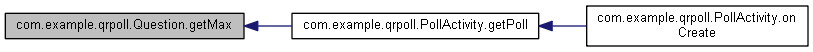
\includegraphics[width=350pt]{classcom_1_1example_1_1qrpoll_1_1_question_a06182185a203fccb72e4421a10a8a511_icgraph}
\end{center}
\end{figure}


\hypertarget{classcom_1_1example_1_1qrpoll_1_1_question_a7b4c664c6c4ebec154ea7132c75bc88d}{\index{com\+::example\+::qrpoll\+::\+Question@{com\+::example\+::qrpoll\+::\+Question}!get\+Pk@{get\+Pk}}
\index{get\+Pk@{get\+Pk}!com\+::example\+::qrpoll\+::\+Question@{com\+::example\+::qrpoll\+::\+Question}}
\subsubsection[{get\+Pk}]{\setlength{\rightskip}{0pt plus 5cm}String com.\+example.\+qrpoll.\+Question.\+get\+Pk (
\begin{DoxyParamCaption}
{}
\end{DoxyParamCaption}
)}}\label{classcom_1_1example_1_1qrpoll_1_1_question_a7b4c664c6c4ebec154ea7132c75bc88d}
\begin{DoxyReturn}{Zwraca}
pk -\/ id pytania 
\end{DoxyReturn}


Definicja w linii 55 pliku Question.\+java.


\begin{DoxyCode}
55                           \{
56         \textcolor{keywordflow}{return} \hyperlink{classcom_1_1example_1_1qrpoll_1_1_question_ab94e31e243d24239faf4ae4c68c28f0b}{pk};
57     \}
\end{DoxyCode}
\hypertarget{classcom_1_1example_1_1qrpoll_1_1_question_ac79778f9afb3c040d0c6f4ada39fb34a}{\index{com\+::example\+::qrpoll\+::\+Question@{com\+::example\+::qrpoll\+::\+Question}!get\+Question\+\_\+text@{get\+Question\+\_\+text}}
\index{get\+Question\+\_\+text@{get\+Question\+\_\+text}!com\+::example\+::qrpoll\+::\+Question@{com\+::example\+::qrpoll\+::\+Question}}
\subsubsection[{get\+Question\+\_\+text}]{\setlength{\rightskip}{0pt plus 5cm}String com.\+example.\+qrpoll.\+Question.\+get\+Question\+\_\+text (
\begin{DoxyParamCaption}
{}
\end{DoxyParamCaption}
)}}\label{classcom_1_1example_1_1qrpoll_1_1_question_ac79778f9afb3c040d0c6f4ada39fb34a}
\begin{DoxyReturn}{Zwraca}

\end{DoxyReturn}


Definicja w linii 68 pliku Question.\+java.


\begin{DoxyCode}
68                                      \{
69         \textcolor{keywordflow}{return} \hyperlink{classcom_1_1example_1_1qrpoll_1_1_question_ab90d61211a23303be8fe8139aed31754}{question\_text};
70     \}
\end{DoxyCode}
\hypertarget{classcom_1_1example_1_1qrpoll_1_1_question_a3608f9d26af608c85ac88ee48e68f624}{\index{com\+::example\+::qrpoll\+::\+Question@{com\+::example\+::qrpoll\+::\+Question}!hash\+Code@{hash\+Code}}
\index{hash\+Code@{hash\+Code}!com\+::example\+::qrpoll\+::\+Question@{com\+::example\+::qrpoll\+::\+Question}}
\subsubsection[{hash\+Code}]{\setlength{\rightskip}{0pt plus 5cm}int com.\+example.\+qrpoll.\+Question.\+hash\+Code (
\begin{DoxyParamCaption}
{}
\end{DoxyParamCaption}
)}}\label{classcom_1_1example_1_1qrpoll_1_1_question_a3608f9d26af608c85ac88ee48e68f624}
\begin{DoxyReturn}{Zwraca}
kod hash pytania 
\end{DoxyReturn}


Definicja w linii 90 pliku Question.\+java.


\begin{DoxyCode}
90                           \{
91         \textcolor{keyword}{final} \textcolor{keywordtype}{int} prime = 31;
92         \textcolor{keywordtype}{int} result = 1;
93         result = prime * result
94                 + ((\hyperlink{classcom_1_1example_1_1qrpoll_1_1_question_aa382153815db46e065ab637ef86f9265}{choice\_map} == null) ? 0 : choice\_map.hashCode());
95         result = prime * result + ((\hyperlink{classcom_1_1example_1_1qrpoll_1_1_question_ab94e31e243d24239faf4ae4c68c28f0b}{pk} == null) ? 0 : pk.hashCode());
96         result = prime * result
97                 + ((\hyperlink{classcom_1_1example_1_1qrpoll_1_1_question_ab90d61211a23303be8fe8139aed31754}{question\_text} == null) ? 0 : question\_text.hashCode());
98         \textcolor{keywordflow}{return} result;
99     \}
\end{DoxyCode}
\hypertarget{classcom_1_1example_1_1qrpoll_1_1_question_aa5e300a74cf22554ee7221da00aff666}{\index{com\+::example\+::qrpoll\+::\+Question@{com\+::example\+::qrpoll\+::\+Question}!is\+Rating@{is\+Rating}}
\index{is\+Rating@{is\+Rating}!com\+::example\+::qrpoll\+::\+Question@{com\+::example\+::qrpoll\+::\+Question}}
\subsubsection[{is\+Rating}]{\setlength{\rightskip}{0pt plus 5cm}String com.\+example.\+qrpoll.\+Question.\+is\+Rating (
\begin{DoxyParamCaption}
{}
\end{DoxyParamCaption}
)}}\label{classcom_1_1example_1_1qrpoll_1_1_question_aa5e300a74cf22554ee7221da00aff666}
zwraca informacje, czy dane pytanie odpowiedzialne jest za ocene spotkania i nie bedzie wyswietlane w glownym layoucie 

Definicja w linii 82 pliku Question.\+java.


\begin{DoxyCode}
82                             \{
83         \textcolor{keywordflow}{return} \hyperlink{classcom_1_1example_1_1qrpoll_1_1_question_aa5e300a74cf22554ee7221da00aff666}{isRating};
84     \}
\end{DoxyCode}


Oto graf wywoływań tej funkcji\+:
\nopagebreak
\begin{figure}[H]
\begin{center}
\leavevmode
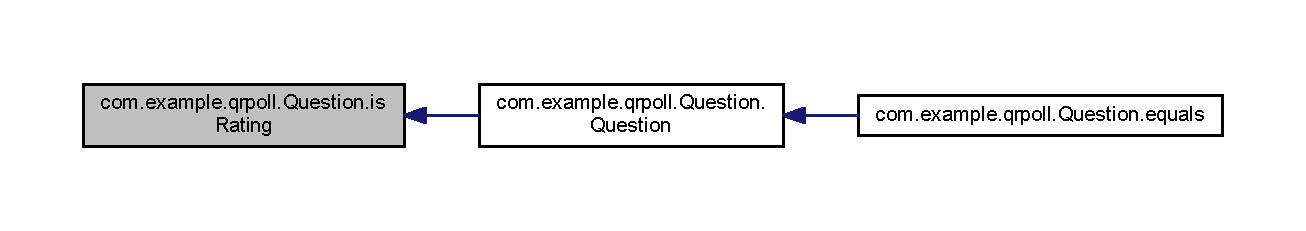
\includegraphics[width=350pt]{classcom_1_1example_1_1qrpoll_1_1_question_aa5e300a74cf22554ee7221da00aff666_icgraph}
\end{center}
\end{figure}




\subsection{Dokumentacja atrybutów składowych}
\hypertarget{classcom_1_1example_1_1qrpoll_1_1_question_aa382153815db46e065ab637ef86f9265}{\index{com\+::example\+::qrpoll\+::\+Question@{com\+::example\+::qrpoll\+::\+Question}!choice\+\_\+map@{choice\+\_\+map}}
\index{choice\+\_\+map@{choice\+\_\+map}!com\+::example\+::qrpoll\+::\+Question@{com\+::example\+::qrpoll\+::\+Question}}
\subsubsection[{choice\+\_\+map}]{\setlength{\rightskip}{0pt plus 5cm}Map$<$String,{\bf Choice}$>$ com.\+example.\+qrpoll.\+Question.\+choice\+\_\+map\hspace{0.3cm}{\ttfamily [private]}}}\label{classcom_1_1example_1_1qrpoll_1_1_question_aa382153815db46e065ab637ef86f9265}


Definicja w linii 27 pliku Question.\+java.

\hypertarget{classcom_1_1example_1_1qrpoll_1_1_question_a7b9016a004baf976a3d700ce332c0e1b}{\index{com\+::example\+::qrpoll\+::\+Question@{com\+::example\+::qrpoll\+::\+Question}!is\+Rating@{is\+Rating}}
\index{is\+Rating@{is\+Rating}!com\+::example\+::qrpoll\+::\+Question@{com\+::example\+::qrpoll\+::\+Question}}
\subsubsection[{is\+Rating}]{\setlength{\rightskip}{0pt plus 5cm}String com.\+example.\+qrpoll.\+Question.\+is\+Rating\hspace{0.3cm}{\ttfamily [private]}}}\label{classcom_1_1example_1_1qrpoll_1_1_question_a7b9016a004baf976a3d700ce332c0e1b}


Definicja w linii 25 pliku Question.\+java.

\hypertarget{classcom_1_1example_1_1qrpoll_1_1_question_a07bd283882253cc7c9ab69718a692a64}{\index{com\+::example\+::qrpoll\+::\+Question@{com\+::example\+::qrpoll\+::\+Question}!max@{max}}
\index{max@{max}!com\+::example\+::qrpoll\+::\+Question@{com\+::example\+::qrpoll\+::\+Question}}
\subsubsection[{max}]{\setlength{\rightskip}{0pt plus 5cm}String com.\+example.\+qrpoll.\+Question.\+max\hspace{0.3cm}{\ttfamily [private]}}}\label{classcom_1_1example_1_1qrpoll_1_1_question_a07bd283882253cc7c9ab69718a692a64}


Definicja w linii 26 pliku Question.\+java.

\hypertarget{classcom_1_1example_1_1qrpoll_1_1_question_ab94e31e243d24239faf4ae4c68c28f0b}{\index{com\+::example\+::qrpoll\+::\+Question@{com\+::example\+::qrpoll\+::\+Question}!pk@{pk}}
\index{pk@{pk}!com\+::example\+::qrpoll\+::\+Question@{com\+::example\+::qrpoll\+::\+Question}}
\subsubsection[{pk}]{\setlength{\rightskip}{0pt plus 5cm}String com.\+example.\+qrpoll.\+Question.\+pk\hspace{0.3cm}{\ttfamily [private]}}}\label{classcom_1_1example_1_1qrpoll_1_1_question_ab94e31e243d24239faf4ae4c68c28f0b}


Definicja w linii 23 pliku Question.\+java.

\hypertarget{classcom_1_1example_1_1qrpoll_1_1_question_ab90d61211a23303be8fe8139aed31754}{\index{com\+::example\+::qrpoll\+::\+Question@{com\+::example\+::qrpoll\+::\+Question}!question\+\_\+text@{question\+\_\+text}}
\index{question\+\_\+text@{question\+\_\+text}!com\+::example\+::qrpoll\+::\+Question@{com\+::example\+::qrpoll\+::\+Question}}
\subsubsection[{question\+\_\+text}]{\setlength{\rightskip}{0pt plus 5cm}String com.\+example.\+qrpoll.\+Question.\+question\+\_\+text\hspace{0.3cm}{\ttfamily [private]}}}\label{classcom_1_1example_1_1qrpoll_1_1_question_ab90d61211a23303be8fe8139aed31754}


Definicja w linii 24 pliku Question.\+java.



Dokumentacja dla tej klasy została wygenerowana z pliku\+:\begin{DoxyCompactItemize}
\item 
C\+:/\+Users/\+Wodzu/\+Documents/\+Git\+Hub/\+Projekt\+Zespolowy/\+Android Final + dokumentacja/android/qrpoll/src/com/example/qrpoll/\hyperlink{_question_8java}{Question.\+java}\end{DoxyCompactItemize}

\hypertarget{classcom_1_1example_1_1qrpoll_1_1_refresh}{\section{Dokumentacja klasy com.\+example.\+qrpoll.\+Refresh}
\label{classcom_1_1example_1_1qrpoll_1_1_refresh}\index{com.\+example.\+qrpoll.\+Refresh@{com.\+example.\+qrpoll.\+Refresh}}
}


Diagram dziedziczenia dla com.\+example.\+qrpoll.\+Refresh
\nopagebreak
\begin{figure}[H]
\begin{center}
\leavevmode
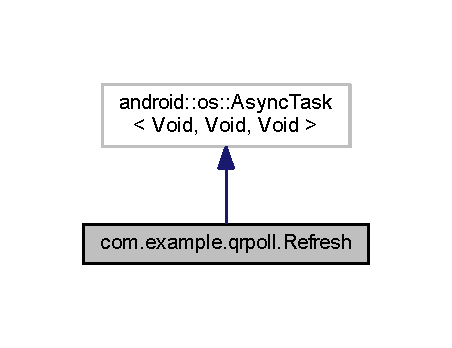
\includegraphics[width=217pt]{classcom_1_1example_1_1qrpoll_1_1_refresh__inherit__graph}
\end{center}
\end{figure}


Diagram współpracy dla com.\+example.\+qrpoll.\+Refresh\+:
\nopagebreak
\begin{figure}[H]
\begin{center}
\leavevmode
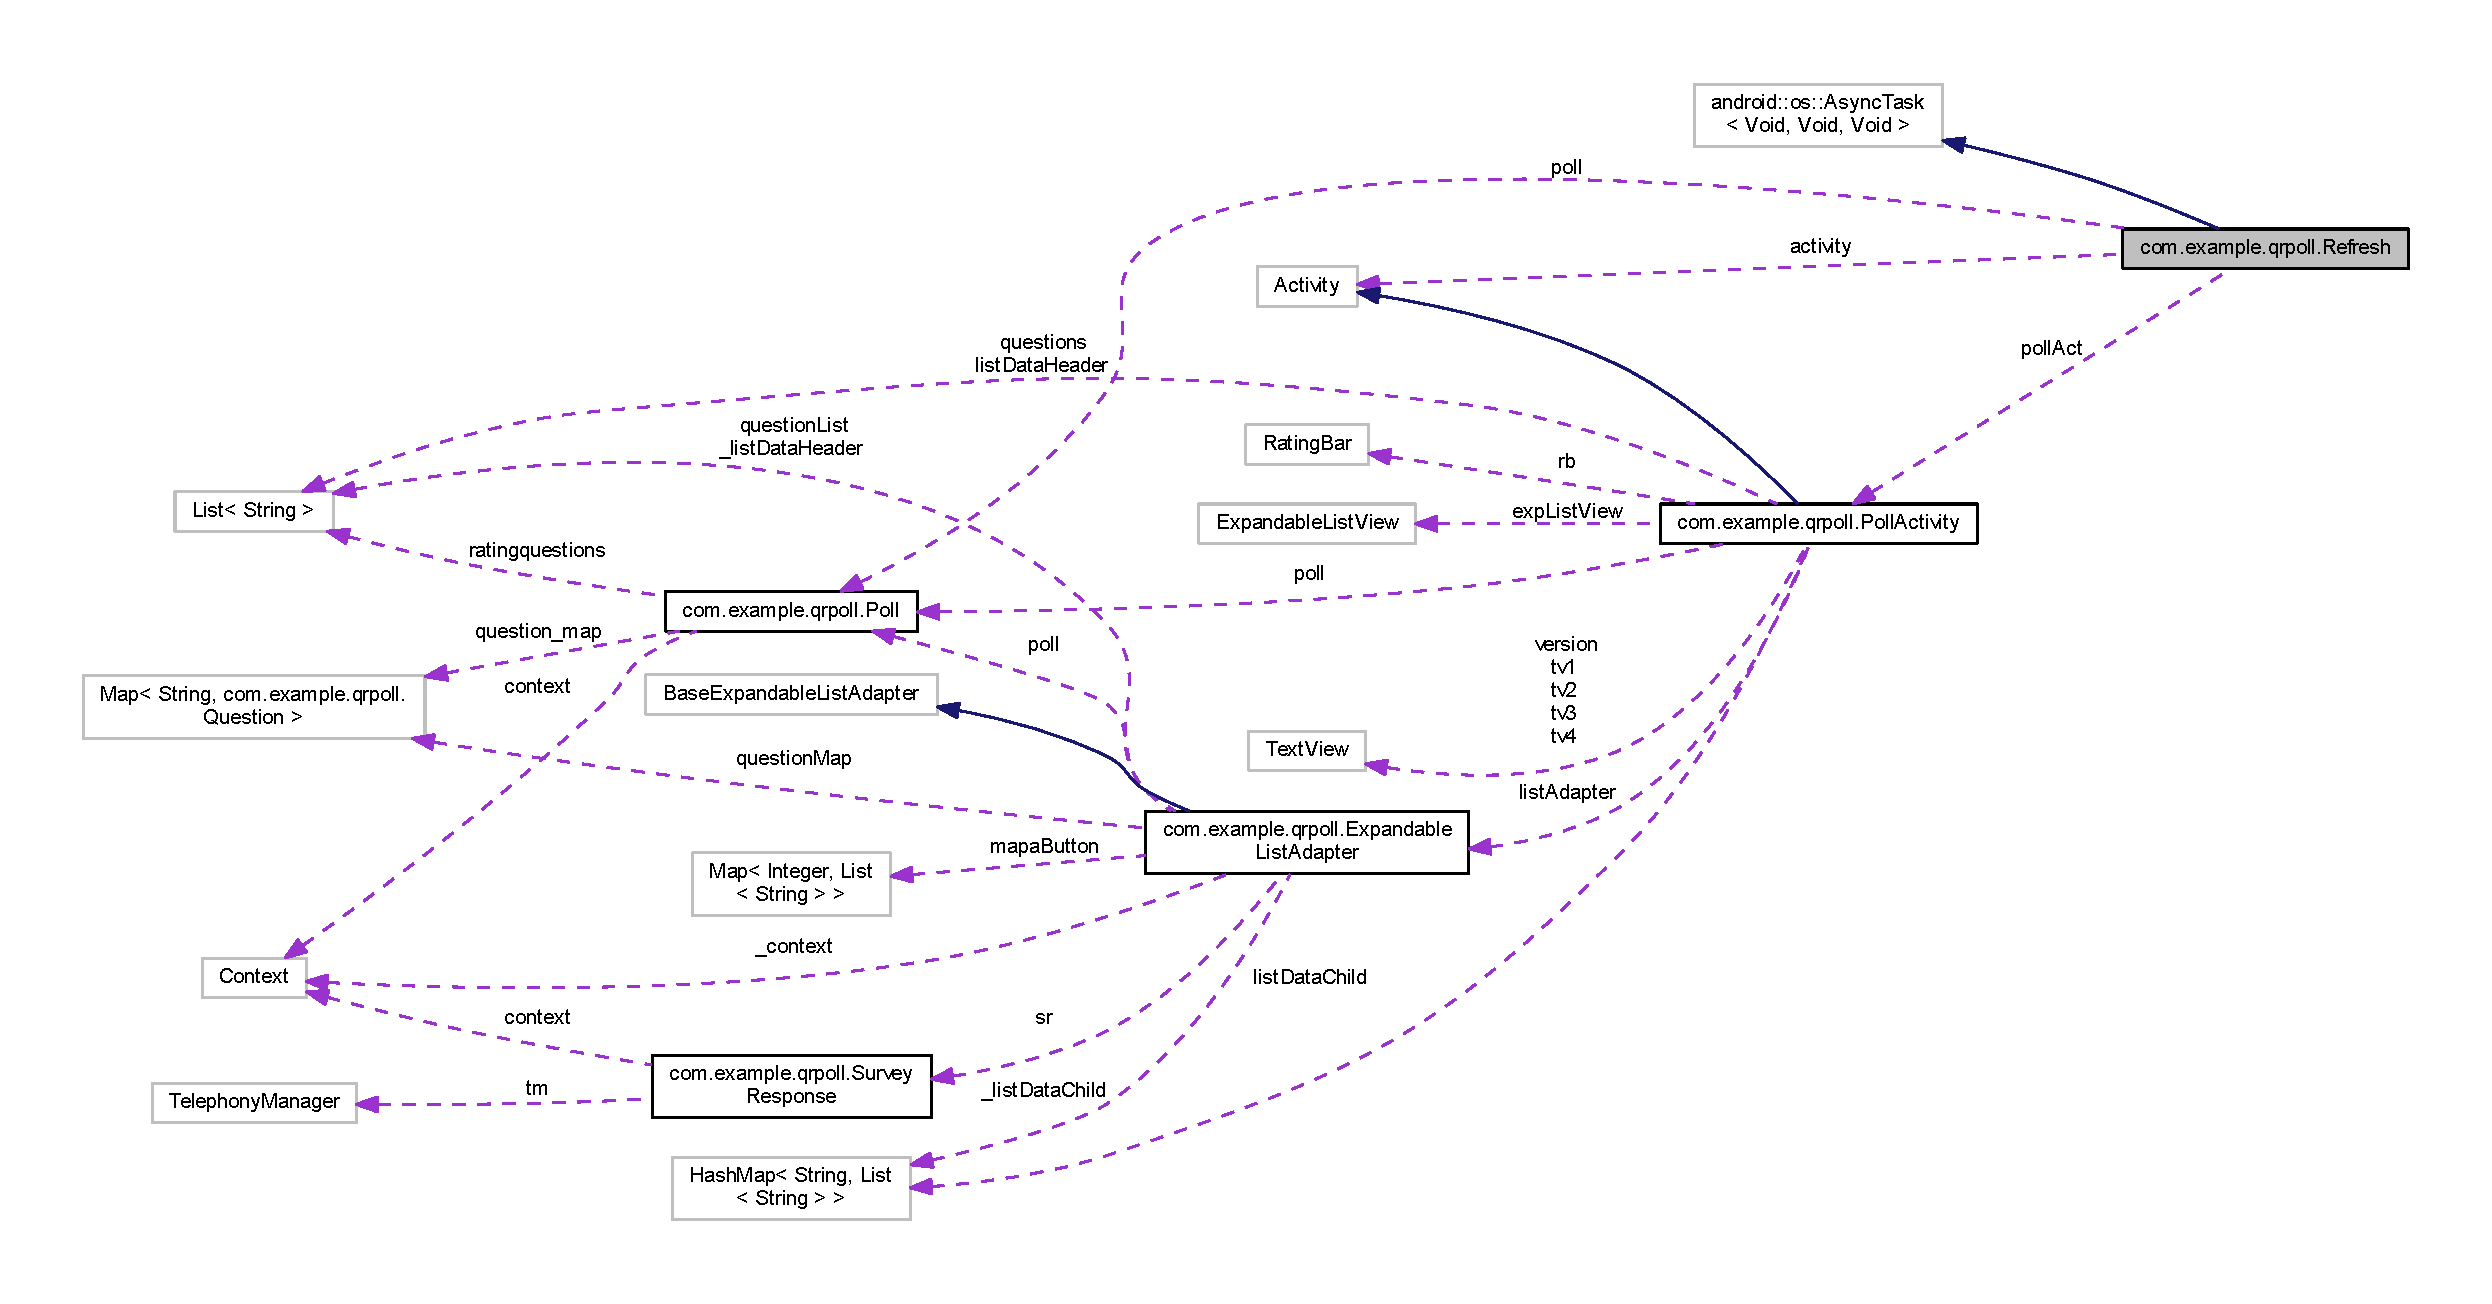
\includegraphics[width=350pt]{classcom_1_1example_1_1qrpoll_1_1_refresh__coll__graph}
\end{center}
\end{figure}
\subsection*{Metody publiczne}
\begin{DoxyCompactItemize}
\item 
\hyperlink{classcom_1_1example_1_1qrpoll_1_1_refresh_a8109c006dde5e3fc97150ac96dde844e}{Refresh} (\hyperlink{classcom_1_1example_1_1qrpoll_1_1_poll}{Poll} \hyperlink{classcom_1_1example_1_1qrpoll_1_1_refresh_a72a1aeb64069e0a0579733c97bb211b3}{poll}, Activity \hyperlink{classcom_1_1example_1_1qrpoll_1_1_refresh_aa3e22cc50197adde6465dd4cb0ce8db5}{activity})
\item 
boolean \hyperlink{classcom_1_1example_1_1qrpoll_1_1_refresh_ab9c3c9d5f96d115b064440c26e4d1260}{check\+Wifi} ()
\item 
boolean \hyperlink{classcom_1_1example_1_1qrpoll_1_1_refresh_ade5487ac2f52c4d306d6c0308c7eae86}{check\+Network} ()
\end{DoxyCompactItemize}
\subsection*{Metody chronione}
\begin{DoxyCompactItemize}
\item 
Void \hyperlink{classcom_1_1example_1_1qrpoll_1_1_refresh_a2f33f8eb0e87c2ed2ff6358486d99424}{do\+In\+Background} (Void...\+arg0)
\end{DoxyCompactItemize}
\subsection*{Atrybuty prywatne}
\begin{DoxyCompactItemize}
\item 
\hyperlink{classcom_1_1example_1_1qrpoll_1_1_poll}{Poll} \hyperlink{classcom_1_1example_1_1qrpoll_1_1_refresh_a72a1aeb64069e0a0579733c97bb211b3}{poll}
\item 
Activity \hyperlink{classcom_1_1example_1_1qrpoll_1_1_refresh_aa3e22cc50197adde6465dd4cb0ce8db5}{activity}
\item 
\hyperlink{classcom_1_1example_1_1qrpoll_1_1_poll_activity}{Poll\+Activity} \hyperlink{classcom_1_1example_1_1qrpoll_1_1_refresh_aa893ac7b613b4da5a7a29dfc3a1bea87}{poll\+Act}
\item 
int \hyperlink{classcom_1_1example_1_1qrpoll_1_1_refresh_ac9c9ddb92776f76a283dd629bf6acbf1}{version}
\end{DoxyCompactItemize}


\subsection{Opis szczegółowy}
\begin{DoxyAuthor}{Autor}
Sliwka klasa obslugujaca sprawdzanie wersji ankiety 
\end{DoxyAuthor}


Definicja w linii 18 pliku Refresh.\+java.



\subsection{Dokumentacja konstruktora i destruktora}
\hypertarget{classcom_1_1example_1_1qrpoll_1_1_refresh_a8109c006dde5e3fc97150ac96dde844e}{\index{com\+::example\+::qrpoll\+::\+Refresh@{com\+::example\+::qrpoll\+::\+Refresh}!Refresh@{Refresh}}
\index{Refresh@{Refresh}!com\+::example\+::qrpoll\+::\+Refresh@{com\+::example\+::qrpoll\+::\+Refresh}}
\subsubsection[{Refresh}]{\setlength{\rightskip}{0pt plus 5cm}com.\+example.\+qrpoll.\+Refresh.\+Refresh (
\begin{DoxyParamCaption}
\item[{{\bf Poll}}]{poll, }
\item[{Activity}]{activity}
\end{DoxyParamCaption}
)}}\label{classcom_1_1example_1_1qrpoll_1_1_refresh_a8109c006dde5e3fc97150ac96dde844e}
glowny konstruktor 
\begin{DoxyParams}{Parametry}
{\em poll} & Aktualna ankieta \\
\hline
{\em activity} & activity ktore wywoluje asynctaska \\
\hline
\end{DoxyParams}


Definicja w linii 28 pliku Refresh.\+java.


\begin{DoxyCode}
28                                                \{
29         this.activity=\hyperlink{classcom_1_1example_1_1qrpoll_1_1_refresh_aa3e22cc50197adde6465dd4cb0ce8db5}{activity};
30         this.poll=\hyperlink{classcom_1_1example_1_1qrpoll_1_1_refresh_a72a1aeb64069e0a0579733c97bb211b3}{poll};
31         this.pollAct=(PollActivity)\hyperlink{classcom_1_1example_1_1qrpoll_1_1_refresh_aa3e22cc50197adde6465dd4cb0ce8db5}{activity};
32     \}
\end{DoxyCode}


\subsection{Dokumentacja funkcji składowych}
\hypertarget{classcom_1_1example_1_1qrpoll_1_1_refresh_ade5487ac2f52c4d306d6c0308c7eae86}{\index{com\+::example\+::qrpoll\+::\+Refresh@{com\+::example\+::qrpoll\+::\+Refresh}!check\+Network@{check\+Network}}
\index{check\+Network@{check\+Network}!com\+::example\+::qrpoll\+::\+Refresh@{com\+::example\+::qrpoll\+::\+Refresh}}
\subsubsection[{check\+Network}]{\setlength{\rightskip}{0pt plus 5cm}boolean com.\+example.\+qrpoll.\+Refresh.\+check\+Network (
\begin{DoxyParamCaption}
{}
\end{DoxyParamCaption}
)}}\label{classcom_1_1example_1_1qrpoll_1_1_refresh_ade5487ac2f52c4d306d6c0308c7eae86}
sprawdzenie danych pakietowych \begin{DoxyReturn}{Zwraca}

\end{DoxyReturn}


Definicja w linii 84 pliku Refresh.\+java.


\begin{DoxyCode}
84                                  \{
85         ConnectivityManager cm=(ConnectivityManager)\hyperlink{classcom_1_1example_1_1qrpoll_1_1_refresh_aa3e22cc50197adde6465dd4cb0ce8db5}{activity}.getApplicationContext()
      .getSystemService(Context.CONNECTIVITY\_SERVICE);
86         NetworkInfo ni=cm.getNetworkInfo(ConnectivityManager.TYPE\_MOBILE);
87         \textcolor{keywordflow}{return} ni.isConnected();
88     \}
\end{DoxyCode}
\hypertarget{classcom_1_1example_1_1qrpoll_1_1_refresh_ab9c3c9d5f96d115b064440c26e4d1260}{\index{com\+::example\+::qrpoll\+::\+Refresh@{com\+::example\+::qrpoll\+::\+Refresh}!check\+Wifi@{check\+Wifi}}
\index{check\+Wifi@{check\+Wifi}!com\+::example\+::qrpoll\+::\+Refresh@{com\+::example\+::qrpoll\+::\+Refresh}}
\subsubsection[{check\+Wifi}]{\setlength{\rightskip}{0pt plus 5cm}boolean com.\+example.\+qrpoll.\+Refresh.\+check\+Wifi (
\begin{DoxyParamCaption}
{}
\end{DoxyParamCaption}
)}}\label{classcom_1_1example_1_1qrpoll_1_1_refresh_ab9c3c9d5f96d115b064440c26e4d1260}
sprawdzenie stanu wifi \begin{DoxyReturn}{Zwraca}

\end{DoxyReturn}


Definicja w linii 76 pliku Refresh.\+java.


\begin{DoxyCode}
76                               \{
77         WifiManager wifi=(WifiManager)\hyperlink{classcom_1_1example_1_1qrpoll_1_1_refresh_aa3e22cc50197adde6465dd4cb0ce8db5}{activity}.getApplicationContext().getSystemService(
      Context.WIFI\_SERVICE);
78         \textcolor{keywordflow}{return} wifi.isWifiEnabled();
79     \}
\end{DoxyCode}
\hypertarget{classcom_1_1example_1_1qrpoll_1_1_refresh_a2f33f8eb0e87c2ed2ff6358486d99424}{\index{com\+::example\+::qrpoll\+::\+Refresh@{com\+::example\+::qrpoll\+::\+Refresh}!do\+In\+Background@{do\+In\+Background}}
\index{do\+In\+Background@{do\+In\+Background}!com\+::example\+::qrpoll\+::\+Refresh@{com\+::example\+::qrpoll\+::\+Refresh}}
\subsubsection[{do\+In\+Background}]{\setlength{\rightskip}{0pt plus 5cm}Void com.\+example.\+qrpoll.\+Refresh.\+do\+In\+Background (
\begin{DoxyParamCaption}
\item[{Void...}]{arg0}
\end{DoxyParamCaption}
)\hspace{0.3cm}{\ttfamily [protected]}}}\label{classcom_1_1example_1_1qrpoll_1_1_refresh_a2f33f8eb0e87c2ed2ff6358486d99424}
sprawdzanie czy nie zmienila sie wersja ankiety 

Definicja w linii 37 pliku Refresh.\+java.


\begin{DoxyCode}
37                                                 \{
38         \textcolor{keywordflow}{while} (!this.isCancelled())\{
39             \textcolor{keywordflow}{try} \{
40                 Thread.sleep(30000);
41                 
42                 \textcolor{comment}{//Toast.makeText(activity.getApplicationContext()," watek dziala",
       Toast.LENGTH\_SHORT).show();}
43                 Log.d(\textcolor{stringliteral}{""}, \textcolor{stringliteral}{"wypisz do logu"});
44             \} \textcolor{keywordflow}{catch} (InterruptedException e) \{
45                 \textcolor{comment}{// TODO Auto-generated catch block}
46                 e.printStackTrace();
47             \}
48             String adress=poll.getAddress();
49             \textcolor{keywordtype}{int} \hyperlink{classcom_1_1example_1_1qrpoll_1_1_refresh_ac9c9ddb92776f76a283dd629bf6acbf1}{version}=poll.getVersion();
50             Poll p=null;
51             \textcolor{keywordflow}{if}(\hyperlink{classcom_1_1example_1_1qrpoll_1_1_refresh_ab9c3c9d5f96d115b064440c26e4d1260}{checkWifi}()||\hyperlink{classcom_1_1example_1_1qrpoll_1_1_refresh_ade5487ac2f52c4d306d6c0308c7eae86}{checkNetwork}())\{
52             \textcolor{keywordflow}{try} \{
53                 p=\textcolor{keyword}{new} Poll(adress,\hyperlink{classcom_1_1example_1_1qrpoll_1_1_refresh_aa3e22cc50197adde6465dd4cb0ce8db5}{activity}.getApplicationContext());
54             \} \textcolor{keywordflow}{catch} (JSONException e) \{
55                 \textcolor{comment}{// TODO Auto-generated catch block}
56                 e.printStackTrace();
57             \}
58             \textcolor{keywordflow}{if}(version!=p.getVersion())\{
59                 this.version=\hyperlink{classcom_1_1example_1_1qrpoll_1_1_refresh_ac9c9ddb92776f76a283dd629bf6acbf1}{version};
60                 pollAct.refresh();
61                 this.cancel(\textcolor{keyword}{true});
62             \}
63             \}\textcolor{keywordflow}{else}\{
64                 \textcolor{comment}{//Toast.makeText(activity.getApplicationContext(),}
65                   \textcolor{comment}{//      "Blad Polaczenia", Toast.LENGTH\_SHORT).show();}
66                 
67                     
68             \}
69         \}
70         \textcolor{keywordflow}{return} null;
71     \}
\end{DoxyCode}


\subsection{Dokumentacja atrybutów składowych}
\hypertarget{classcom_1_1example_1_1qrpoll_1_1_refresh_aa3e22cc50197adde6465dd4cb0ce8db5}{\index{com\+::example\+::qrpoll\+::\+Refresh@{com\+::example\+::qrpoll\+::\+Refresh}!activity@{activity}}
\index{activity@{activity}!com\+::example\+::qrpoll\+::\+Refresh@{com\+::example\+::qrpoll\+::\+Refresh}}
\subsubsection[{activity}]{\setlength{\rightskip}{0pt plus 5cm}Activity com.\+example.\+qrpoll.\+Refresh.\+activity\hspace{0.3cm}{\ttfamily [private]}}}\label{classcom_1_1example_1_1qrpoll_1_1_refresh_aa3e22cc50197adde6465dd4cb0ce8db5}


Definicja w linii 20 pliku Refresh.\+java.

\hypertarget{classcom_1_1example_1_1qrpoll_1_1_refresh_a72a1aeb64069e0a0579733c97bb211b3}{\index{com\+::example\+::qrpoll\+::\+Refresh@{com\+::example\+::qrpoll\+::\+Refresh}!poll@{poll}}
\index{poll@{poll}!com\+::example\+::qrpoll\+::\+Refresh@{com\+::example\+::qrpoll\+::\+Refresh}}
\subsubsection[{poll}]{\setlength{\rightskip}{0pt plus 5cm}{\bf Poll} com.\+example.\+qrpoll.\+Refresh.\+poll\hspace{0.3cm}{\ttfamily [private]}}}\label{classcom_1_1example_1_1qrpoll_1_1_refresh_a72a1aeb64069e0a0579733c97bb211b3}


Definicja w linii 19 pliku Refresh.\+java.

\hypertarget{classcom_1_1example_1_1qrpoll_1_1_refresh_aa893ac7b613b4da5a7a29dfc3a1bea87}{\index{com\+::example\+::qrpoll\+::\+Refresh@{com\+::example\+::qrpoll\+::\+Refresh}!poll\+Act@{poll\+Act}}
\index{poll\+Act@{poll\+Act}!com\+::example\+::qrpoll\+::\+Refresh@{com\+::example\+::qrpoll\+::\+Refresh}}
\subsubsection[{poll\+Act}]{\setlength{\rightskip}{0pt plus 5cm}{\bf Poll\+Activity} com.\+example.\+qrpoll.\+Refresh.\+poll\+Act\hspace{0.3cm}{\ttfamily [private]}}}\label{classcom_1_1example_1_1qrpoll_1_1_refresh_aa893ac7b613b4da5a7a29dfc3a1bea87}


Definicja w linii 21 pliku Refresh.\+java.

\hypertarget{classcom_1_1example_1_1qrpoll_1_1_refresh_ac9c9ddb92776f76a283dd629bf6acbf1}{\index{com\+::example\+::qrpoll\+::\+Refresh@{com\+::example\+::qrpoll\+::\+Refresh}!version@{version}}
\index{version@{version}!com\+::example\+::qrpoll\+::\+Refresh@{com\+::example\+::qrpoll\+::\+Refresh}}
\subsubsection[{version}]{\setlength{\rightskip}{0pt plus 5cm}int com.\+example.\+qrpoll.\+Refresh.\+version\hspace{0.3cm}{\ttfamily [private]}}}\label{classcom_1_1example_1_1qrpoll_1_1_refresh_ac9c9ddb92776f76a283dd629bf6acbf1}


Definicja w linii 22 pliku Refresh.\+java.



Dokumentacja dla tej klasy została wygenerowana z pliku\+:\begin{DoxyCompactItemize}
\item 
\hyperlink{_refresh_8java}{Refresh.\+java}\end{DoxyCompactItemize}

\hypertarget{classcom_1_1example_1_1qrpoll_1_1_sql_handler}{\section{Dokumentacja klasy com.\+example.\+qrpoll.\+Sql\+Handler}
\label{classcom_1_1example_1_1qrpoll_1_1_sql_handler}\index{com.\+example.\+qrpoll.\+Sql\+Handler@{com.\+example.\+qrpoll.\+Sql\+Handler}}
}


Diagram współpracy dla com.\+example.\+qrpoll.\+Sql\+Handler\+:
\nopagebreak
\begin{figure}[H]
\begin{center}
\leavevmode
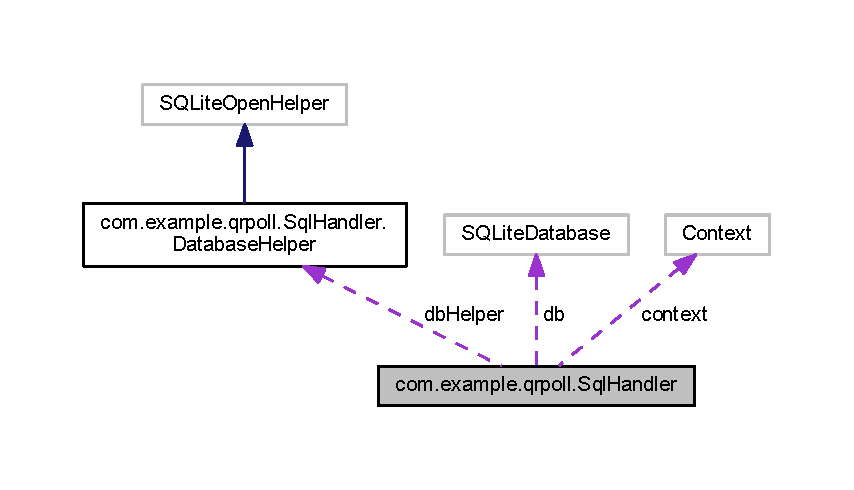
\includegraphics[width=350pt]{classcom_1_1example_1_1qrpoll_1_1_sql_handler__coll__graph}
\end{center}
\end{figure}
\subsection*{Komponenty}
\begin{DoxyCompactItemize}
\item 
class \hyperlink{classcom_1_1example_1_1qrpoll_1_1_sql_handler_1_1_database_helper}{Database\+Helper}
\end{DoxyCompactItemize}
\subsection*{Metody publiczne}
\begin{DoxyCompactItemize}
\item 
\hyperlink{classcom_1_1example_1_1qrpoll_1_1_sql_handler_a53ed47985d1fc8282e594bd646d10f10}{Sql\+Handler} (Context \hyperlink{classcom_1_1example_1_1qrpoll_1_1_sql_handler_ab0071f750233a8b37790758a430d847c}{context})
\item 
\hyperlink{classcom_1_1example_1_1qrpoll_1_1_sql_handler}{Sql\+Handler} \hyperlink{classcom_1_1example_1_1qrpoll_1_1_sql_handler_a8ff4b44bac212ce1711edd40331c5f3a}{open} ()
\item 
void \hyperlink{classcom_1_1example_1_1qrpoll_1_1_sql_handler_afab084d101af94d630e4cad2e2d0aad6}{close} ()
\item 
long \hyperlink{classcom_1_1example_1_1qrpoll_1_1_sql_handler_a277e4b5d26c99949e13a5a522662f579}{insert\+Spotkania} (String hash, String subject, String room, String date)
\item 
Cursor \hyperlink{classcom_1_1example_1_1qrpoll_1_1_sql_handler_a36835546e39ab97bd1473650c86eebfb}{get\+Data\+From\+Spotkanie} ()
\item 
Cursor \hyperlink{classcom_1_1example_1_1qrpoll_1_1_sql_handler_a75a37c2aaac5411dd77de0df7b07acc7}{get\+Data\+With\+Specific\+Id} (int id)
\item 
Cursor \hyperlink{classcom_1_1example_1_1qrpoll_1_1_sql_handler_a2c5fa84b5eb6c9f28e1519c663501e60}{get\+Data\+With\+Specific\+Hash} (String hash)
\item 
Array\+List$<$ \hyperlink{classcom_1_1example_1_1qrpoll_1_1_item}{Item} $>$ \hyperlink{classcom_1_1example_1_1qrpoll_1_1_sql_handler_ab6085ad33e5f50aa8c3d84d35f62728c}{get\+All} ()
\end{DoxyCompactItemize}
\subsection*{Statyczne atrybuty publiczne}
\begin{DoxyCompactItemize}
\item 
static final String \hyperlink{classcom_1_1example_1_1qrpoll_1_1_sql_handler_ac68ddd9373f28e201126af152708a978}{K\+E\+Y\+\_\+\+I\+D} =\char`\"{}id\char`\"{}
\item 
static final String \hyperlink{classcom_1_1example_1_1qrpoll_1_1_sql_handler_aa5a0c822d90c20141ddadf6a396c332f}{I\+D\+\_\+\+O\+P\+T\+I\+O\+N} =\char`\"{}I\+N\+T\+E\+G\+E\+R P\+R\+I\+M\+A\+R\+Y K\+E\+Y A\+U\+T\+O\+I\+N\+C\+R\+E\+M\+E\+N\+T\char`\"{}
\item 
static final int \hyperlink{classcom_1_1example_1_1qrpoll_1_1_sql_handler_a2c504a59b0a9b6b99a26b181fa875460}{I\+D\+\_\+\+C\+O\+L\+U\+M\+N} =0
\item 
static final String \hyperlink{classcom_1_1example_1_1qrpoll_1_1_sql_handler_a300c5ab4aec2e6338f2ca3477c86821b}{K\+E\+Y\+\_\+\+H\+A\+S\+H} =\char`\"{}hash\char`\"{}
\item 
static final String \hyperlink{classcom_1_1example_1_1qrpoll_1_1_sql_handler_a5e06705347d09bc8a2a42b18b7ae2a39}{H\+A\+S\+H\+\_\+\+O\+P\+T\+I\+O\+N} =\char`\"{}T\+E\+X\+T N\+O\+T N\+U\+L\+L\char`\"{}
\item 
static final int \hyperlink{classcom_1_1example_1_1qrpoll_1_1_sql_handler_abec6f5e9cb2ce511c936dc1ae80c83f0}{H\+A\+S\+H\+\_\+\+C\+O\+L\+U\+M\+N} =1
\item 
static final String \hyperlink{classcom_1_1example_1_1qrpoll_1_1_sql_handler_a5f388a6da5567ff51d36f49536889787}{K\+E\+Y\+\_\+\+S\+U\+B\+J\+E\+C\+T} =\char`\"{}subject\char`\"{}
\item 
static final String \hyperlink{classcom_1_1example_1_1qrpoll_1_1_sql_handler_a285e762c9eafe65d7fd408a27909fe31}{S\+U\+B\+J\+E\+C\+T\+\_\+\+O\+P\+T\+I\+O\+N} =\char`\"{}T\+E\+X\+T N\+O\+T N\+U\+L\+L\char`\"{}
\item 
static final int \hyperlink{classcom_1_1example_1_1qrpoll_1_1_sql_handler_a8aceb6280c8a2a0b343b7e20f29b6a21}{S\+U\+B\+J\+E\+C\+T\+\_\+\+C\+O\+L\+U\+M\+N} =2
\item 
static final String \hyperlink{classcom_1_1example_1_1qrpoll_1_1_sql_handler_a78fbe309193399fb67d76eadb67f4b33}{K\+E\+Y\+\_\+\+R\+O\+O\+M} =\char`\"{}room\char`\"{}
\item 
static final String \hyperlink{classcom_1_1example_1_1qrpoll_1_1_sql_handler_a7c6a68ef75025eb240b041ea3f005e46}{R\+O\+O\+M\+\_\+\+O\+P\+T\+I\+O\+N} =\char`\"{}T\+E\+X\+T N\+O\+T N\+U\+L\+L\char`\"{}
\item 
static final int \hyperlink{classcom_1_1example_1_1qrpoll_1_1_sql_handler_aca9368d9d6803238b65e853fcf32a5aa}{R\+O\+O\+M\+\_\+\+C\+O\+L\+U\+M\+N} =3
\item 
static final String \hyperlink{classcom_1_1example_1_1qrpoll_1_1_sql_handler_a93e50d5f5a35250e6655f1d8f3192975}{K\+E\+Y\+\_\+\+D\+A\+T\+E} =\char`\"{}date\char`\"{}
\item 
static final String \hyperlink{classcom_1_1example_1_1qrpoll_1_1_sql_handler_a1d7af0faf52a8e5ba92eac4595bbb94c}{D\+A\+T\+E\+\_\+\+O\+P\+T\+I\+O\+N} =\char`\"{}T\+E\+X\+T N\+O\+T N\+U\+L\+L\char`\"{}
\item 
static final int \hyperlink{classcom_1_1example_1_1qrpoll_1_1_sql_handler_ad3e3a44b82059d37635eda84d51228e6}{D\+A\+T\+E\+\_\+\+C\+O\+L\+U\+M\+N} =4
\end{DoxyCompactItemize}
\subsection*{Atrybuty prywatne}
\begin{DoxyCompactItemize}
\item 
S\+Q\+Lite\+Database \hyperlink{classcom_1_1example_1_1qrpoll_1_1_sql_handler_a5b422e7952698eb1df158709d4e18007}{db}
\item 
Context \hyperlink{classcom_1_1example_1_1qrpoll_1_1_sql_handler_ab0071f750233a8b37790758a430d847c}{context}
\item 
\hyperlink{classcom_1_1example_1_1qrpoll_1_1_sql_handler_1_1_database_helper}{Database\+Helper} \hyperlink{classcom_1_1example_1_1qrpoll_1_1_sql_handler_a70cd37adedee066fc05708b0990c4f6c}{db\+Helper}
\end{DoxyCompactItemize}
\subsection*{Statyczne atrybuty prywatne}
\begin{DoxyCompactItemize}
\item 
static final int \hyperlink{classcom_1_1example_1_1qrpoll_1_1_sql_handler_a10db6c9a4c952c10c3e67c633797a244}{D\+B\+\_\+\+V\+E\+R\+S\+I\+O\+N} =1
\item 
static final String \hyperlink{classcom_1_1example_1_1qrpoll_1_1_sql_handler_a1e5b9131804451b9c7e6e9cd0eeb7187}{D\+B\+\_\+\+N\+A\+M\+E} =\char`\"{}database.\+db\char`\"{}
\item 
static final String \hyperlink{classcom_1_1example_1_1qrpoll_1_1_sql_handler_a5858d638c1d649a755b4f18614481a48}{D\+B\+\_\+\+T\+A\+B\+L\+E\+\_\+1} =\char`\"{}spotkania\char`\"{}
\item 
static final String \hyperlink{classcom_1_1example_1_1qrpoll_1_1_sql_handler_a41cc7444128cfe954cd829ceb98d8df0}{Create\+\_\+table\+\_\+spotkania}
\item 
static final String \hyperlink{classcom_1_1example_1_1qrpoll_1_1_sql_handler_afed000c5d08d75442fbb860297d5d8b1}{Drop\+\_\+table\+\_\+spotkania} =\char`\"{}D\+R\+O\+P T\+A\+B\+L\+E I\+F E\+X\+I\+S\+T\+S \char`\"{}+D\+B\+\_\+\+T\+A\+B\+L\+E\+\_\+1
\end{DoxyCompactItemize}


\subsection{Opis szczegółowy}
klasa do obslugi lokalnej bazy danych, zawiera jedna tabele \+:Spotkanie \begin{DoxyAuthor}{Autor}
sliwka 
\end{DoxyAuthor}


Definicja w linii 19 pliku Sql\+Handler.\+java.



\subsection{Dokumentacja konstruktora i destruktora}
\hypertarget{classcom_1_1example_1_1qrpoll_1_1_sql_handler_a53ed47985d1fc8282e594bd646d10f10}{\index{com\+::example\+::qrpoll\+::\+Sql\+Handler@{com\+::example\+::qrpoll\+::\+Sql\+Handler}!Sql\+Handler@{Sql\+Handler}}
\index{Sql\+Handler@{Sql\+Handler}!com\+::example\+::qrpoll\+::\+Sql\+Handler@{com\+::example\+::qrpoll\+::\+Sql\+Handler}}
\subsubsection[{Sql\+Handler}]{\setlength{\rightskip}{0pt plus 5cm}com.\+example.\+qrpoll.\+Sql\+Handler.\+Sql\+Handler (
\begin{DoxyParamCaption}
\item[{Context}]{context}
\end{DoxyParamCaption}
)}}\label{classcom_1_1example_1_1qrpoll_1_1_sql_handler_a53ed47985d1fc8282e594bd646d10f10}

\begin{DoxyParams}{Parametry}
{\em context} & \\
\hline
\end{DoxyParams}


Definicja w linii 27 pliku Sql\+Handler.\+java.


\begin{DoxyCode}
27                                           \{
28             this.context=\hyperlink{classcom_1_1example_1_1qrpoll_1_1_sql_handler_ab0071f750233a8b37790758a430d847c}{context};
29         \}
\end{DoxyCode}


\subsection{Dokumentacja funkcji składowych}
\hypertarget{classcom_1_1example_1_1qrpoll_1_1_sql_handler_afab084d101af94d630e4cad2e2d0aad6}{\index{com\+::example\+::qrpoll\+::\+Sql\+Handler@{com\+::example\+::qrpoll\+::\+Sql\+Handler}!close@{close}}
\index{close@{close}!com\+::example\+::qrpoll\+::\+Sql\+Handler@{com\+::example\+::qrpoll\+::\+Sql\+Handler}}
\subsubsection[{close}]{\setlength{\rightskip}{0pt plus 5cm}void com.\+example.\+qrpoll.\+Sql\+Handler.\+close (
\begin{DoxyParamCaption}
{}
\end{DoxyParamCaption}
)}}\label{classcom_1_1example_1_1qrpoll_1_1_sql_handler_afab084d101af94d630e4cad2e2d0aad6}
zamykanie polaczenia z baza 

Definicja w linii 46 pliku Sql\+Handler.\+java.


\begin{DoxyCode}
46                            \{
47             dbHelper.close();
48         \}
\end{DoxyCode}
\hypertarget{classcom_1_1example_1_1qrpoll_1_1_sql_handler_ab6085ad33e5f50aa8c3d84d35f62728c}{\index{com\+::example\+::qrpoll\+::\+Sql\+Handler@{com\+::example\+::qrpoll\+::\+Sql\+Handler}!get\+All@{get\+All}}
\index{get\+All@{get\+All}!com\+::example\+::qrpoll\+::\+Sql\+Handler@{com\+::example\+::qrpoll\+::\+Sql\+Handler}}
\subsubsection[{get\+All}]{\setlength{\rightskip}{0pt plus 5cm}Array\+List$<${\bf Item}$>$ com.\+example.\+qrpoll.\+Sql\+Handler.\+get\+All (
\begin{DoxyParamCaption}
{}
\end{DoxyParamCaption}
)}}\label{classcom_1_1example_1_1qrpoll_1_1_sql_handler_ab6085ad33e5f50aa8c3d84d35f62728c}
Metoda zwracajaca liste wszystkich krotek \begin{DoxyReturn}{Zwraca}

\end{DoxyReturn}


Definicja w linii 135 pliku Sql\+Handler.\+java.


\begin{DoxyCode}
135                                        \{
136             ArrayList<Item>list=\textcolor{keyword}{new} ArrayList<Item>();
137             String[]columns=\{\hyperlink{classcom_1_1example_1_1qrpoll_1_1_sql_handler_ac68ddd9373f28e201126af152708a978}{KEY\_ID},\hyperlink{classcom_1_1example_1_1qrpoll_1_1_sql_handler_a300c5ab4aec2e6338f2ca3477c86821b}{KEY\_HASH},\hyperlink{classcom_1_1example_1_1qrpoll_1_1_sql_handler_a5f388a6da5567ff51d36f49536889787}{KEY\_SUBJECT},
      \hyperlink{classcom_1_1example_1_1qrpoll_1_1_sql_handler_a78fbe309193399fb67d76eadb67f4b33}{KEY\_ROOM},\hyperlink{classcom_1_1example_1_1qrpoll_1_1_sql_handler_a93e50d5f5a35250e6655f1d8f3192975}{KEY\_DATE}\};
138             Cursor csr=db.query(\hyperlink{classcom_1_1example_1_1qrpoll_1_1_sql_handler_a5858d638c1d649a755b4f18614481a48}{DB\_TABLE\_1}, columns, null, null, null, null, null);
139             \textcolor{keywordflow}{while}(csr.moveToNext())\{
140                 Item item=\textcolor{keyword}{new} Item(csr.getString(\hyperlink{classcom_1_1example_1_1qrpoll_1_1_sql_handler_a8aceb6280c8a2a0b343b7e20f29b6a21}{SUBJECT\_COLUMN}),csr.getString(
      \hyperlink{classcom_1_1example_1_1qrpoll_1_1_sql_handler_abec6f5e9cb2ce511c936dc1ae80c83f0}{HASH\_COLUMN}),csr.getString(\hyperlink{classcom_1_1example_1_1qrpoll_1_1_sql_handler_ad3e3a44b82059d37635eda84d51228e6}{DATE\_COLUMN}),csr.getString(
      \hyperlink{classcom_1_1example_1_1qrpoll_1_1_sql_handler_aca9368d9d6803238b65e853fcf32a5aa}{ROOM\_COLUMN}));
141                 list.add(item);
142             \}
143             \textcolor{keywordflow}{return} list;
144         \}
\end{DoxyCode}
\hypertarget{classcom_1_1example_1_1qrpoll_1_1_sql_handler_a36835546e39ab97bd1473650c86eebfb}{\index{com\+::example\+::qrpoll\+::\+Sql\+Handler@{com\+::example\+::qrpoll\+::\+Sql\+Handler}!get\+Data\+From\+Spotkanie@{get\+Data\+From\+Spotkanie}}
\index{get\+Data\+From\+Spotkanie@{get\+Data\+From\+Spotkanie}!com\+::example\+::qrpoll\+::\+Sql\+Handler@{com\+::example\+::qrpoll\+::\+Sql\+Handler}}
\subsubsection[{get\+Data\+From\+Spotkanie}]{\setlength{\rightskip}{0pt plus 5cm}Cursor com.\+example.\+qrpoll.\+Sql\+Handler.\+get\+Data\+From\+Spotkanie (
\begin{DoxyParamCaption}
{}
\end{DoxyParamCaption}
)}}\label{classcom_1_1example_1_1qrpoll_1_1_sql_handler_a36835546e39ab97bd1473650c86eebfb}
Metoda wyciagajaca rekordy z bazy danych \begin{DoxyReturn}{Zwraca}
Kursor zawierajacy wszystkie rekordy z bazy 
\end{DoxyReturn}


Definicja w linii 107 pliku Sql\+Handler.\+java.


\begin{DoxyCode}
107                                             \{
108             String[]columns=\{\hyperlink{classcom_1_1example_1_1qrpoll_1_1_sql_handler_ac68ddd9373f28e201126af152708a978}{KEY\_ID},\hyperlink{classcom_1_1example_1_1qrpoll_1_1_sql_handler_a300c5ab4aec2e6338f2ca3477c86821b}{KEY\_HASH},\hyperlink{classcom_1_1example_1_1qrpoll_1_1_sql_handler_a5f388a6da5567ff51d36f49536889787}{KEY\_SUBJECT},
      \hyperlink{classcom_1_1example_1_1qrpoll_1_1_sql_handler_a78fbe309193399fb67d76eadb67f4b33}{KEY\_ROOM},\hyperlink{classcom_1_1example_1_1qrpoll_1_1_sql_handler_a93e50d5f5a35250e6655f1d8f3192975}{KEY\_DATE}\};
109             \textcolor{keywordflow}{return} db.query(\hyperlink{classcom_1_1example_1_1qrpoll_1_1_sql_handler_a5858d638c1d649a755b4f18614481a48}{DB\_TABLE\_1}, columns, null, null, null, null, null);
110         \}
\end{DoxyCode}
\hypertarget{classcom_1_1example_1_1qrpoll_1_1_sql_handler_a2c5fa84b5eb6c9f28e1519c663501e60}{\index{com\+::example\+::qrpoll\+::\+Sql\+Handler@{com\+::example\+::qrpoll\+::\+Sql\+Handler}!get\+Data\+With\+Specific\+Hash@{get\+Data\+With\+Specific\+Hash}}
\index{get\+Data\+With\+Specific\+Hash@{get\+Data\+With\+Specific\+Hash}!com\+::example\+::qrpoll\+::\+Sql\+Handler@{com\+::example\+::qrpoll\+::\+Sql\+Handler}}
\subsubsection[{get\+Data\+With\+Specific\+Hash}]{\setlength{\rightskip}{0pt plus 5cm}Cursor com.\+example.\+qrpoll.\+Sql\+Handler.\+get\+Data\+With\+Specific\+Hash (
\begin{DoxyParamCaption}
\item[{String}]{hash}
\end{DoxyParamCaption}
)}}\label{classcom_1_1example_1_1qrpoll_1_1_sql_handler_a2c5fa84b5eb6c9f28e1519c663501e60}
Metoda wyciagajaca z bazy rekordy o podanym hashu 
\begin{DoxyParams}{Parametry}
{\em hash} & \\
\hline
\end{DoxyParams}
\begin{DoxyReturn}{Zwraca}

\end{DoxyReturn}


Definicja w linii 126 pliku Sql\+Handler.\+java.


\begin{DoxyCode}
126                                                           \{
127             String[]columns=\{\hyperlink{classcom_1_1example_1_1qrpoll_1_1_sql_handler_ac68ddd9373f28e201126af152708a978}{KEY\_ID}\};
128             String where=\hyperlink{classcom_1_1example_1_1qrpoll_1_1_sql_handler_a300c5ab4aec2e6338f2ca3477c86821b}{KEY\_HASH}+\textcolor{stringliteral}{"='"}+hash+\textcolor{stringliteral}{"'"};
129             \textcolor{keywordflow}{return} db.query(\hyperlink{classcom_1_1example_1_1qrpoll_1_1_sql_handler_a5858d638c1d649a755b4f18614481a48}{DB\_TABLE\_1}, columns, where, null, null, null, null);
130         \}
\end{DoxyCode}
\hypertarget{classcom_1_1example_1_1qrpoll_1_1_sql_handler_a75a37c2aaac5411dd77de0df7b07acc7}{\index{com\+::example\+::qrpoll\+::\+Sql\+Handler@{com\+::example\+::qrpoll\+::\+Sql\+Handler}!get\+Data\+With\+Specific\+Id@{get\+Data\+With\+Specific\+Id}}
\index{get\+Data\+With\+Specific\+Id@{get\+Data\+With\+Specific\+Id}!com\+::example\+::qrpoll\+::\+Sql\+Handler@{com\+::example\+::qrpoll\+::\+Sql\+Handler}}
\subsubsection[{get\+Data\+With\+Specific\+Id}]{\setlength{\rightskip}{0pt plus 5cm}Cursor com.\+example.\+qrpoll.\+Sql\+Handler.\+get\+Data\+With\+Specific\+Id (
\begin{DoxyParamCaption}
\item[{int}]{id}
\end{DoxyParamCaption}
)}}\label{classcom_1_1example_1_1qrpoll_1_1_sql_handler_a75a37c2aaac5411dd77de0df7b07acc7}
Metoda wyciagajaca z bazy rekordy o podanym id 
\begin{DoxyParams}{Parametry}
{\em id} & \\
\hline
\end{DoxyParams}
\begin{DoxyReturn}{Zwraca}
Kursor zawierajacy rekordy 
\end{DoxyReturn}


Definicja w linii 116 pliku Sql\+Handler.\+java.


\begin{DoxyCode}
116                                                    \{
117             String[]columns=\{\hyperlink{classcom_1_1example_1_1qrpoll_1_1_sql_handler_ac68ddd9373f28e201126af152708a978}{KEY\_ID},\hyperlink{classcom_1_1example_1_1qrpoll_1_1_sql_handler_a300c5ab4aec2e6338f2ca3477c86821b}{KEY\_HASH},\hyperlink{classcom_1_1example_1_1qrpoll_1_1_sql_handler_a5f388a6da5567ff51d36f49536889787}{KEY\_SUBJECT},
      \hyperlink{classcom_1_1example_1_1qrpoll_1_1_sql_handler_a78fbe309193399fb67d76eadb67f4b33}{KEY\_ROOM},\hyperlink{classcom_1_1example_1_1qrpoll_1_1_sql_handler_a93e50d5f5a35250e6655f1d8f3192975}{KEY\_DATE}\};
118             String where=\hyperlink{classcom_1_1example_1_1qrpoll_1_1_sql_handler_ac68ddd9373f28e201126af152708a978}{KEY\_ID} + \textcolor{stringliteral}{"="} + id;
119             \textcolor{keywordflow}{return} db.query(\hyperlink{classcom_1_1example_1_1qrpoll_1_1_sql_handler_a5858d638c1d649a755b4f18614481a48}{DB\_TABLE\_1}, columns, where, null, null, null, null);
120         \}
\end{DoxyCode}
\hypertarget{classcom_1_1example_1_1qrpoll_1_1_sql_handler_a277e4b5d26c99949e13a5a522662f579}{\index{com\+::example\+::qrpoll\+::\+Sql\+Handler@{com\+::example\+::qrpoll\+::\+Sql\+Handler}!insert\+Spotkania@{insert\+Spotkania}}
\index{insert\+Spotkania@{insert\+Spotkania}!com\+::example\+::qrpoll\+::\+Sql\+Handler@{com\+::example\+::qrpoll\+::\+Sql\+Handler}}
\subsubsection[{insert\+Spotkania}]{\setlength{\rightskip}{0pt plus 5cm}long com.\+example.\+qrpoll.\+Sql\+Handler.\+insert\+Spotkania (
\begin{DoxyParamCaption}
\item[{String}]{hash, }
\item[{String}]{subject, }
\item[{String}]{room, }
\item[{String}]{date}
\end{DoxyParamCaption}
)}}\label{classcom_1_1example_1_1qrpoll_1_1_sql_handler_a277e4b5d26c99949e13a5a522662f579}
Wstawianie danych do bazy 
\begin{DoxyParams}{Parametry}
{\em hash} & \\
\hline
{\em subject} & \\
\hline
{\em room} & \\
\hline
{\em date} & \\
\hline
\end{DoxyParams}
\begin{DoxyReturn}{Zwraca}
id wstawianej krotki 
\end{DoxyReturn}


Definicja w linii 89 pliku Sql\+Handler.\+java.


\begin{DoxyCode}
89                                                                                         \{
90             ContentValues newSpotkanieValues = \textcolor{keyword}{new} ContentValues();
91             newSpotkanieValues.put(\hyperlink{classcom_1_1example_1_1qrpoll_1_1_sql_handler_a300c5ab4aec2e6338f2ca3477c86821b}{KEY\_HASH}, hash);
92             newSpotkanieValues.put(\hyperlink{classcom_1_1example_1_1qrpoll_1_1_sql_handler_a5f388a6da5567ff51d36f49536889787}{KEY\_SUBJECT}, subject);
93             newSpotkanieValues.put(\hyperlink{classcom_1_1example_1_1qrpoll_1_1_sql_handler_a78fbe309193399fb67d76eadb67f4b33}{KEY\_ROOM}, room);
94             newSpotkanieValues.put(\hyperlink{classcom_1_1example_1_1qrpoll_1_1_sql_handler_a93e50d5f5a35250e6655f1d8f3192975}{KEY\_DATE}, date);
95             Cursor cursor=\hyperlink{classcom_1_1example_1_1qrpoll_1_1_sql_handler_a2c5fa84b5eb6c9f28e1519c663501e60}{getDataWithSpecificHash}(hash);
96             \textcolor{keywordflow}{if}(cursor.getCount()==0)\{
97                 Log.d(\textcolor{stringliteral}{"SqLiteTodoManager"}, \textcolor{stringliteral}{"not exists"});
98                 \textcolor{keywordflow}{return} db.insert(\hyperlink{classcom_1_1example_1_1qrpoll_1_1_sql_handler_a5858d638c1d649a755b4f18614481a48}{DB\_TABLE\_1}, null, newSpotkanieValues);
99             \}
100             
101             \textcolor{keywordflow}{return} -1;
102         \}
\end{DoxyCode}
\hypertarget{classcom_1_1example_1_1qrpoll_1_1_sql_handler_a8ff4b44bac212ce1711edd40331c5f3a}{\index{com\+::example\+::qrpoll\+::\+Sql\+Handler@{com\+::example\+::qrpoll\+::\+Sql\+Handler}!open@{open}}
\index{open@{open}!com\+::example\+::qrpoll\+::\+Sql\+Handler@{com\+::example\+::qrpoll\+::\+Sql\+Handler}}
\subsubsection[{open}]{\setlength{\rightskip}{0pt plus 5cm}{\bf Sql\+Handler} com.\+example.\+qrpoll.\+Sql\+Handler.\+open (
\begin{DoxyParamCaption}
{}
\end{DoxyParamCaption}
)}}\label{classcom_1_1example_1_1qrpoll_1_1_sql_handler_a8ff4b44bac212ce1711edd40331c5f3a}
Nawiazywanie polaczenia z baza danych sqlite \begin{DoxyReturn}{Zwraca}

\end{DoxyReturn}


Definicja w linii 34 pliku Sql\+Handler.\+java.


\begin{DoxyCode}
34                                 \{
35             \hyperlink{classcom_1_1example_1_1qrpoll_1_1_sql_handler_a70cd37adedee066fc05708b0990c4f6c}{dbHelper}=\textcolor{keyword}{new} DatabaseHelper(\hyperlink{classcom_1_1example_1_1qrpoll_1_1_sql_handler_ab0071f750233a8b37790758a430d847c}{context},\hyperlink{classcom_1_1example_1_1qrpoll_1_1_sql_handler_a1e5b9131804451b9c7e6e9cd0eeb7187}{DB\_NAME},null,
      \hyperlink{classcom_1_1example_1_1qrpoll_1_1_sql_handler_a10db6c9a4c952c10c3e67c633797a244}{DB\_VERSION});
36             \textcolor{keywordflow}{try}\{
37                 \hyperlink{classcom_1_1example_1_1qrpoll_1_1_sql_handler_a5b422e7952698eb1df158709d4e18007}{db}=dbHelper.getWritableDatabase();
38             \}\textcolor{keywordflow}{catch}(SQLException e)\{
39                 \hyperlink{classcom_1_1example_1_1qrpoll_1_1_sql_handler_a5b422e7952698eb1df158709d4e18007}{db}=dbHelper.getReadableDatabase();
40             \}
41             \textcolor{keywordflow}{return} \textcolor{keyword}{this};
42         \}
\end{DoxyCode}


\subsection{Dokumentacja atrybutów składowych}
\hypertarget{classcom_1_1example_1_1qrpoll_1_1_sql_handler_ab0071f750233a8b37790758a430d847c}{\index{com\+::example\+::qrpoll\+::\+Sql\+Handler@{com\+::example\+::qrpoll\+::\+Sql\+Handler}!context@{context}}
\index{context@{context}!com\+::example\+::qrpoll\+::\+Sql\+Handler@{com\+::example\+::qrpoll\+::\+Sql\+Handler}}
\subsubsection[{context}]{\setlength{\rightskip}{0pt plus 5cm}Context com.\+example.\+qrpoll.\+Sql\+Handler.\+context\hspace{0.3cm}{\ttfamily [private]}}}\label{classcom_1_1example_1_1qrpoll_1_1_sql_handler_ab0071f750233a8b37790758a430d847c}


Definicja w linii 21 pliku Sql\+Handler.\+java.

\hypertarget{classcom_1_1example_1_1qrpoll_1_1_sql_handler_a41cc7444128cfe954cd829ceb98d8df0}{\index{com\+::example\+::qrpoll\+::\+Sql\+Handler@{com\+::example\+::qrpoll\+::\+Sql\+Handler}!Create\+\_\+table\+\_\+spotkania@{Create\+\_\+table\+\_\+spotkania}}
\index{Create\+\_\+table\+\_\+spotkania@{Create\+\_\+table\+\_\+spotkania}!com\+::example\+::qrpoll\+::\+Sql\+Handler@{com\+::example\+::qrpoll\+::\+Sql\+Handler}}
\subsubsection[{Create\+\_\+table\+\_\+spotkania}]{\setlength{\rightskip}{0pt plus 5cm}final String com.\+example.\+qrpoll.\+Sql\+Handler.\+Create\+\_\+table\+\_\+spotkania\hspace{0.3cm}{\ttfamily [static]}, {\ttfamily [private]}}}\label{classcom_1_1example_1_1qrpoll_1_1_sql_handler_a41cc7444128cfe954cd829ceb98d8df0}
{\bfseries Wartość początkowa\+:}
\begin{DoxyCode}
=\textcolor{stringliteral}{"CREATE TABLE IF NOT EXISTS "}+\hyperlink{classcom_1_1example_1_1qrpoll_1_1_sql_handler_a5858d638c1d649a755b4f18614481a48}{DB\_TABLE\_1}+\textcolor{stringliteral}{"("}
                +\hyperlink{classcom_1_1example_1_1qrpoll_1_1_sql_handler_ac68ddd9373f28e201126af152708a978}{KEY\_ID}+ \textcolor{stringliteral}{" "}+\hyperlink{classcom_1_1example_1_1qrpoll_1_1_sql_handler_aa5a0c822d90c20141ddadf6a396c332f}{ID\_OPTION}+\textcolor{stringliteral}{","}+\hyperlink{classcom_1_1example_1_1qrpoll_1_1_sql_handler_a300c5ab4aec2e6338f2ca3477c86821b}{KEY\_HASH}+ \textcolor{stringliteral}{" "}+
      \hyperlink{classcom_1_1example_1_1qrpoll_1_1_sql_handler_a5e06705347d09bc8a2a42b18b7ae2a39}{HASH\_OPTION}+\textcolor{stringliteral}{","}+\hyperlink{classcom_1_1example_1_1qrpoll_1_1_sql_handler_a5f388a6da5567ff51d36f49536889787}{KEY\_SUBJECT}+ \textcolor{stringliteral}{" "}+\hyperlink{classcom_1_1example_1_1qrpoll_1_1_sql_handler_a285e762c9eafe65d7fd408a27909fe31}{SUBJECT\_OPTION}+\textcolor{stringliteral}{","}
                +\hyperlink{classcom_1_1example_1_1qrpoll_1_1_sql_handler_a78fbe309193399fb67d76eadb67f4b33}{KEY\_ROOM}+ \textcolor{stringliteral}{" "}+\hyperlink{classcom_1_1example_1_1qrpoll_1_1_sql_handler_a7c6a68ef75025eb240b041ea3f005e46}{ROOM\_OPTION}+\textcolor{stringliteral}{","}+\hyperlink{classcom_1_1example_1_1qrpoll_1_1_sql_handler_a93e50d5f5a35250e6655f1d8f3192975}{KEY\_DATE}+ \textcolor{stringliteral}{" "}+
      \hyperlink{classcom_1_1example_1_1qrpoll_1_1_sql_handler_a1d7af0faf52a8e5ba92eac4595bbb94c}{DATE\_OPTION}+\textcolor{stringliteral}{")"}
\end{DoxyCode}


Definicja w linii 73 pliku Sql\+Handler.\+java.

\hypertarget{classcom_1_1example_1_1qrpoll_1_1_sql_handler_ad3e3a44b82059d37635eda84d51228e6}{\index{com\+::example\+::qrpoll\+::\+Sql\+Handler@{com\+::example\+::qrpoll\+::\+Sql\+Handler}!D\+A\+T\+E\+\_\+\+C\+O\+L\+U\+M\+N@{D\+A\+T\+E\+\_\+\+C\+O\+L\+U\+M\+N}}
\index{D\+A\+T\+E\+\_\+\+C\+O\+L\+U\+M\+N@{D\+A\+T\+E\+\_\+\+C\+O\+L\+U\+M\+N}!com\+::example\+::qrpoll\+::\+Sql\+Handler@{com\+::example\+::qrpoll\+::\+Sql\+Handler}}
\subsubsection[{D\+A\+T\+E\+\_\+\+C\+O\+L\+U\+M\+N}]{\setlength{\rightskip}{0pt plus 5cm}final int com.\+example.\+qrpoll.\+Sql\+Handler.\+D\+A\+T\+E\+\_\+\+C\+O\+L\+U\+M\+N =4\hspace{0.3cm}{\ttfamily [static]}}}\label{classcom_1_1example_1_1qrpoll_1_1_sql_handler_ad3e3a44b82059d37635eda84d51228e6}


Definicja w linii 71 pliku Sql\+Handler.\+java.

\hypertarget{classcom_1_1example_1_1qrpoll_1_1_sql_handler_a1d7af0faf52a8e5ba92eac4595bbb94c}{\index{com\+::example\+::qrpoll\+::\+Sql\+Handler@{com\+::example\+::qrpoll\+::\+Sql\+Handler}!D\+A\+T\+E\+\_\+\+O\+P\+T\+I\+O\+N@{D\+A\+T\+E\+\_\+\+O\+P\+T\+I\+O\+N}}
\index{D\+A\+T\+E\+\_\+\+O\+P\+T\+I\+O\+N@{D\+A\+T\+E\+\_\+\+O\+P\+T\+I\+O\+N}!com\+::example\+::qrpoll\+::\+Sql\+Handler@{com\+::example\+::qrpoll\+::\+Sql\+Handler}}
\subsubsection[{D\+A\+T\+E\+\_\+\+O\+P\+T\+I\+O\+N}]{\setlength{\rightskip}{0pt plus 5cm}final String com.\+example.\+qrpoll.\+Sql\+Handler.\+D\+A\+T\+E\+\_\+\+O\+P\+T\+I\+O\+N =\char`\"{}T\+E\+X\+T N\+O\+T N\+U\+L\+L\char`\"{}\hspace{0.3cm}{\ttfamily [static]}}}\label{classcom_1_1example_1_1qrpoll_1_1_sql_handler_a1d7af0faf52a8e5ba92eac4595bbb94c}


Definicja w linii 70 pliku Sql\+Handler.\+java.

\hypertarget{classcom_1_1example_1_1qrpoll_1_1_sql_handler_a5b422e7952698eb1df158709d4e18007}{\index{com\+::example\+::qrpoll\+::\+Sql\+Handler@{com\+::example\+::qrpoll\+::\+Sql\+Handler}!db@{db}}
\index{db@{db}!com\+::example\+::qrpoll\+::\+Sql\+Handler@{com\+::example\+::qrpoll\+::\+Sql\+Handler}}
\subsubsection[{db}]{\setlength{\rightskip}{0pt plus 5cm}S\+Q\+Lite\+Database com.\+example.\+qrpoll.\+Sql\+Handler.\+db\hspace{0.3cm}{\ttfamily [private]}}}\label{classcom_1_1example_1_1qrpoll_1_1_sql_handler_a5b422e7952698eb1df158709d4e18007}


Definicja w linii 20 pliku Sql\+Handler.\+java.

\hypertarget{classcom_1_1example_1_1qrpoll_1_1_sql_handler_a1e5b9131804451b9c7e6e9cd0eeb7187}{\index{com\+::example\+::qrpoll\+::\+Sql\+Handler@{com\+::example\+::qrpoll\+::\+Sql\+Handler}!D\+B\+\_\+\+N\+A\+M\+E@{D\+B\+\_\+\+N\+A\+M\+E}}
\index{D\+B\+\_\+\+N\+A\+M\+E@{D\+B\+\_\+\+N\+A\+M\+E}!com\+::example\+::qrpoll\+::\+Sql\+Handler@{com\+::example\+::qrpoll\+::\+Sql\+Handler}}
\subsubsection[{D\+B\+\_\+\+N\+A\+M\+E}]{\setlength{\rightskip}{0pt plus 5cm}final String com.\+example.\+qrpoll.\+Sql\+Handler.\+D\+B\+\_\+\+N\+A\+M\+E =\char`\"{}database.\+db\char`\"{}\hspace{0.3cm}{\ttfamily [static]}, {\ttfamily [private]}}}\label{classcom_1_1example_1_1qrpoll_1_1_sql_handler_a1e5b9131804451b9c7e6e9cd0eeb7187}


Definicja w linii 50 pliku Sql\+Handler.\+java.

\hypertarget{classcom_1_1example_1_1qrpoll_1_1_sql_handler_a5858d638c1d649a755b4f18614481a48}{\index{com\+::example\+::qrpoll\+::\+Sql\+Handler@{com\+::example\+::qrpoll\+::\+Sql\+Handler}!D\+B\+\_\+\+T\+A\+B\+L\+E\+\_\+1@{D\+B\+\_\+\+T\+A\+B\+L\+E\+\_\+1}}
\index{D\+B\+\_\+\+T\+A\+B\+L\+E\+\_\+1@{D\+B\+\_\+\+T\+A\+B\+L\+E\+\_\+1}!com\+::example\+::qrpoll\+::\+Sql\+Handler@{com\+::example\+::qrpoll\+::\+Sql\+Handler}}
\subsubsection[{D\+B\+\_\+\+T\+A\+B\+L\+E\+\_\+1}]{\setlength{\rightskip}{0pt plus 5cm}final String com.\+example.\+qrpoll.\+Sql\+Handler.\+D\+B\+\_\+\+T\+A\+B\+L\+E\+\_\+1 =\char`\"{}spotkania\char`\"{}\hspace{0.3cm}{\ttfamily [static]}, {\ttfamily [private]}}}\label{classcom_1_1example_1_1qrpoll_1_1_sql_handler_a5858d638c1d649a755b4f18614481a48}


Definicja w linii 51 pliku Sql\+Handler.\+java.

\hypertarget{classcom_1_1example_1_1qrpoll_1_1_sql_handler_a10db6c9a4c952c10c3e67c633797a244}{\index{com\+::example\+::qrpoll\+::\+Sql\+Handler@{com\+::example\+::qrpoll\+::\+Sql\+Handler}!D\+B\+\_\+\+V\+E\+R\+S\+I\+O\+N@{D\+B\+\_\+\+V\+E\+R\+S\+I\+O\+N}}
\index{D\+B\+\_\+\+V\+E\+R\+S\+I\+O\+N@{D\+B\+\_\+\+V\+E\+R\+S\+I\+O\+N}!com\+::example\+::qrpoll\+::\+Sql\+Handler@{com\+::example\+::qrpoll\+::\+Sql\+Handler}}
\subsubsection[{D\+B\+\_\+\+V\+E\+R\+S\+I\+O\+N}]{\setlength{\rightskip}{0pt plus 5cm}final int com.\+example.\+qrpoll.\+Sql\+Handler.\+D\+B\+\_\+\+V\+E\+R\+S\+I\+O\+N =1\hspace{0.3cm}{\ttfamily [static]}, {\ttfamily [private]}}}\label{classcom_1_1example_1_1qrpoll_1_1_sql_handler_a10db6c9a4c952c10c3e67c633797a244}


Definicja w linii 49 pliku Sql\+Handler.\+java.

\hypertarget{classcom_1_1example_1_1qrpoll_1_1_sql_handler_a70cd37adedee066fc05708b0990c4f6c}{\index{com\+::example\+::qrpoll\+::\+Sql\+Handler@{com\+::example\+::qrpoll\+::\+Sql\+Handler}!db\+Helper@{db\+Helper}}
\index{db\+Helper@{db\+Helper}!com\+::example\+::qrpoll\+::\+Sql\+Handler@{com\+::example\+::qrpoll\+::\+Sql\+Handler}}
\subsubsection[{db\+Helper}]{\setlength{\rightskip}{0pt plus 5cm}{\bf Database\+Helper} com.\+example.\+qrpoll.\+Sql\+Handler.\+db\+Helper\hspace{0.3cm}{\ttfamily [private]}}}\label{classcom_1_1example_1_1qrpoll_1_1_sql_handler_a70cd37adedee066fc05708b0990c4f6c}


Definicja w linii 22 pliku Sql\+Handler.\+java.

\hypertarget{classcom_1_1example_1_1qrpoll_1_1_sql_handler_afed000c5d08d75442fbb860297d5d8b1}{\index{com\+::example\+::qrpoll\+::\+Sql\+Handler@{com\+::example\+::qrpoll\+::\+Sql\+Handler}!Drop\+\_\+table\+\_\+spotkania@{Drop\+\_\+table\+\_\+spotkania}}
\index{Drop\+\_\+table\+\_\+spotkania@{Drop\+\_\+table\+\_\+spotkania}!com\+::example\+::qrpoll\+::\+Sql\+Handler@{com\+::example\+::qrpoll\+::\+Sql\+Handler}}
\subsubsection[{Drop\+\_\+table\+\_\+spotkania}]{\setlength{\rightskip}{0pt plus 5cm}final String com.\+example.\+qrpoll.\+Sql\+Handler.\+Drop\+\_\+table\+\_\+spotkania =\char`\"{}D\+R\+O\+P T\+A\+B\+L\+E I\+F E\+X\+I\+S\+T\+S \char`\"{}+D\+B\+\_\+\+T\+A\+B\+L\+E\+\_\+1\hspace{0.3cm}{\ttfamily [static]}, {\ttfamily [private]}}}\label{classcom_1_1example_1_1qrpoll_1_1_sql_handler_afed000c5d08d75442fbb860297d5d8b1}


Definicja w linii 79 pliku Sql\+Handler.\+java.

\hypertarget{classcom_1_1example_1_1qrpoll_1_1_sql_handler_abec6f5e9cb2ce511c936dc1ae80c83f0}{\index{com\+::example\+::qrpoll\+::\+Sql\+Handler@{com\+::example\+::qrpoll\+::\+Sql\+Handler}!H\+A\+S\+H\+\_\+\+C\+O\+L\+U\+M\+N@{H\+A\+S\+H\+\_\+\+C\+O\+L\+U\+M\+N}}
\index{H\+A\+S\+H\+\_\+\+C\+O\+L\+U\+M\+N@{H\+A\+S\+H\+\_\+\+C\+O\+L\+U\+M\+N}!com\+::example\+::qrpoll\+::\+Sql\+Handler@{com\+::example\+::qrpoll\+::\+Sql\+Handler}}
\subsubsection[{H\+A\+S\+H\+\_\+\+C\+O\+L\+U\+M\+N}]{\setlength{\rightskip}{0pt plus 5cm}final int com.\+example.\+qrpoll.\+Sql\+Handler.\+H\+A\+S\+H\+\_\+\+C\+O\+L\+U\+M\+N =1\hspace{0.3cm}{\ttfamily [static]}}}\label{classcom_1_1example_1_1qrpoll_1_1_sql_handler_abec6f5e9cb2ce511c936dc1ae80c83f0}


Definicja w linii 59 pliku Sql\+Handler.\+java.

\hypertarget{classcom_1_1example_1_1qrpoll_1_1_sql_handler_a5e06705347d09bc8a2a42b18b7ae2a39}{\index{com\+::example\+::qrpoll\+::\+Sql\+Handler@{com\+::example\+::qrpoll\+::\+Sql\+Handler}!H\+A\+S\+H\+\_\+\+O\+P\+T\+I\+O\+N@{H\+A\+S\+H\+\_\+\+O\+P\+T\+I\+O\+N}}
\index{H\+A\+S\+H\+\_\+\+O\+P\+T\+I\+O\+N@{H\+A\+S\+H\+\_\+\+O\+P\+T\+I\+O\+N}!com\+::example\+::qrpoll\+::\+Sql\+Handler@{com\+::example\+::qrpoll\+::\+Sql\+Handler}}
\subsubsection[{H\+A\+S\+H\+\_\+\+O\+P\+T\+I\+O\+N}]{\setlength{\rightskip}{0pt plus 5cm}final String com.\+example.\+qrpoll.\+Sql\+Handler.\+H\+A\+S\+H\+\_\+\+O\+P\+T\+I\+O\+N =\char`\"{}T\+E\+X\+T N\+O\+T N\+U\+L\+L\char`\"{}\hspace{0.3cm}{\ttfamily [static]}}}\label{classcom_1_1example_1_1qrpoll_1_1_sql_handler_a5e06705347d09bc8a2a42b18b7ae2a39}


Definicja w linii 58 pliku Sql\+Handler.\+java.

\hypertarget{classcom_1_1example_1_1qrpoll_1_1_sql_handler_a2c504a59b0a9b6b99a26b181fa875460}{\index{com\+::example\+::qrpoll\+::\+Sql\+Handler@{com\+::example\+::qrpoll\+::\+Sql\+Handler}!I\+D\+\_\+\+C\+O\+L\+U\+M\+N@{I\+D\+\_\+\+C\+O\+L\+U\+M\+N}}
\index{I\+D\+\_\+\+C\+O\+L\+U\+M\+N@{I\+D\+\_\+\+C\+O\+L\+U\+M\+N}!com\+::example\+::qrpoll\+::\+Sql\+Handler@{com\+::example\+::qrpoll\+::\+Sql\+Handler}}
\subsubsection[{I\+D\+\_\+\+C\+O\+L\+U\+M\+N}]{\setlength{\rightskip}{0pt plus 5cm}final int com.\+example.\+qrpoll.\+Sql\+Handler.\+I\+D\+\_\+\+C\+O\+L\+U\+M\+N =0\hspace{0.3cm}{\ttfamily [static]}}}\label{classcom_1_1example_1_1qrpoll_1_1_sql_handler_a2c504a59b0a9b6b99a26b181fa875460}


Definicja w linii 55 pliku Sql\+Handler.\+java.

\hypertarget{classcom_1_1example_1_1qrpoll_1_1_sql_handler_aa5a0c822d90c20141ddadf6a396c332f}{\index{com\+::example\+::qrpoll\+::\+Sql\+Handler@{com\+::example\+::qrpoll\+::\+Sql\+Handler}!I\+D\+\_\+\+O\+P\+T\+I\+O\+N@{I\+D\+\_\+\+O\+P\+T\+I\+O\+N}}
\index{I\+D\+\_\+\+O\+P\+T\+I\+O\+N@{I\+D\+\_\+\+O\+P\+T\+I\+O\+N}!com\+::example\+::qrpoll\+::\+Sql\+Handler@{com\+::example\+::qrpoll\+::\+Sql\+Handler}}
\subsubsection[{I\+D\+\_\+\+O\+P\+T\+I\+O\+N}]{\setlength{\rightskip}{0pt plus 5cm}final String com.\+example.\+qrpoll.\+Sql\+Handler.\+I\+D\+\_\+\+O\+P\+T\+I\+O\+N =\char`\"{}I\+N\+T\+E\+G\+E\+R P\+R\+I\+M\+A\+R\+Y K\+E\+Y A\+U\+T\+O\+I\+N\+C\+R\+E\+M\+E\+N\+T\char`\"{}\hspace{0.3cm}{\ttfamily [static]}}}\label{classcom_1_1example_1_1qrpoll_1_1_sql_handler_aa5a0c822d90c20141ddadf6a396c332f}


Definicja w linii 54 pliku Sql\+Handler.\+java.

\hypertarget{classcom_1_1example_1_1qrpoll_1_1_sql_handler_a93e50d5f5a35250e6655f1d8f3192975}{\index{com\+::example\+::qrpoll\+::\+Sql\+Handler@{com\+::example\+::qrpoll\+::\+Sql\+Handler}!K\+E\+Y\+\_\+\+D\+A\+T\+E@{K\+E\+Y\+\_\+\+D\+A\+T\+E}}
\index{K\+E\+Y\+\_\+\+D\+A\+T\+E@{K\+E\+Y\+\_\+\+D\+A\+T\+E}!com\+::example\+::qrpoll\+::\+Sql\+Handler@{com\+::example\+::qrpoll\+::\+Sql\+Handler}}
\subsubsection[{K\+E\+Y\+\_\+\+D\+A\+T\+E}]{\setlength{\rightskip}{0pt plus 5cm}final String com.\+example.\+qrpoll.\+Sql\+Handler.\+K\+E\+Y\+\_\+\+D\+A\+T\+E =\char`\"{}date\char`\"{}\hspace{0.3cm}{\ttfamily [static]}}}\label{classcom_1_1example_1_1qrpoll_1_1_sql_handler_a93e50d5f5a35250e6655f1d8f3192975}


Definicja w linii 69 pliku Sql\+Handler.\+java.

\hypertarget{classcom_1_1example_1_1qrpoll_1_1_sql_handler_a300c5ab4aec2e6338f2ca3477c86821b}{\index{com\+::example\+::qrpoll\+::\+Sql\+Handler@{com\+::example\+::qrpoll\+::\+Sql\+Handler}!K\+E\+Y\+\_\+\+H\+A\+S\+H@{K\+E\+Y\+\_\+\+H\+A\+S\+H}}
\index{K\+E\+Y\+\_\+\+H\+A\+S\+H@{K\+E\+Y\+\_\+\+H\+A\+S\+H}!com\+::example\+::qrpoll\+::\+Sql\+Handler@{com\+::example\+::qrpoll\+::\+Sql\+Handler}}
\subsubsection[{K\+E\+Y\+\_\+\+H\+A\+S\+H}]{\setlength{\rightskip}{0pt plus 5cm}final String com.\+example.\+qrpoll.\+Sql\+Handler.\+K\+E\+Y\+\_\+\+H\+A\+S\+H =\char`\"{}hash\char`\"{}\hspace{0.3cm}{\ttfamily [static]}}}\label{classcom_1_1example_1_1qrpoll_1_1_sql_handler_a300c5ab4aec2e6338f2ca3477c86821b}


Definicja w linii 57 pliku Sql\+Handler.\+java.

\hypertarget{classcom_1_1example_1_1qrpoll_1_1_sql_handler_ac68ddd9373f28e201126af152708a978}{\index{com\+::example\+::qrpoll\+::\+Sql\+Handler@{com\+::example\+::qrpoll\+::\+Sql\+Handler}!K\+E\+Y\+\_\+\+I\+D@{K\+E\+Y\+\_\+\+I\+D}}
\index{K\+E\+Y\+\_\+\+I\+D@{K\+E\+Y\+\_\+\+I\+D}!com\+::example\+::qrpoll\+::\+Sql\+Handler@{com\+::example\+::qrpoll\+::\+Sql\+Handler}}
\subsubsection[{K\+E\+Y\+\_\+\+I\+D}]{\setlength{\rightskip}{0pt plus 5cm}final String com.\+example.\+qrpoll.\+Sql\+Handler.\+K\+E\+Y\+\_\+\+I\+D =\char`\"{}id\char`\"{}\hspace{0.3cm}{\ttfamily [static]}}}\label{classcom_1_1example_1_1qrpoll_1_1_sql_handler_ac68ddd9373f28e201126af152708a978}


Definicja w linii 53 pliku Sql\+Handler.\+java.

\hypertarget{classcom_1_1example_1_1qrpoll_1_1_sql_handler_a78fbe309193399fb67d76eadb67f4b33}{\index{com\+::example\+::qrpoll\+::\+Sql\+Handler@{com\+::example\+::qrpoll\+::\+Sql\+Handler}!K\+E\+Y\+\_\+\+R\+O\+O\+M@{K\+E\+Y\+\_\+\+R\+O\+O\+M}}
\index{K\+E\+Y\+\_\+\+R\+O\+O\+M@{K\+E\+Y\+\_\+\+R\+O\+O\+M}!com\+::example\+::qrpoll\+::\+Sql\+Handler@{com\+::example\+::qrpoll\+::\+Sql\+Handler}}
\subsubsection[{K\+E\+Y\+\_\+\+R\+O\+O\+M}]{\setlength{\rightskip}{0pt plus 5cm}final String com.\+example.\+qrpoll.\+Sql\+Handler.\+K\+E\+Y\+\_\+\+R\+O\+O\+M =\char`\"{}room\char`\"{}\hspace{0.3cm}{\ttfamily [static]}}}\label{classcom_1_1example_1_1qrpoll_1_1_sql_handler_a78fbe309193399fb67d76eadb67f4b33}


Definicja w linii 65 pliku Sql\+Handler.\+java.

\hypertarget{classcom_1_1example_1_1qrpoll_1_1_sql_handler_a5f388a6da5567ff51d36f49536889787}{\index{com\+::example\+::qrpoll\+::\+Sql\+Handler@{com\+::example\+::qrpoll\+::\+Sql\+Handler}!K\+E\+Y\+\_\+\+S\+U\+B\+J\+E\+C\+T@{K\+E\+Y\+\_\+\+S\+U\+B\+J\+E\+C\+T}}
\index{K\+E\+Y\+\_\+\+S\+U\+B\+J\+E\+C\+T@{K\+E\+Y\+\_\+\+S\+U\+B\+J\+E\+C\+T}!com\+::example\+::qrpoll\+::\+Sql\+Handler@{com\+::example\+::qrpoll\+::\+Sql\+Handler}}
\subsubsection[{K\+E\+Y\+\_\+\+S\+U\+B\+J\+E\+C\+T}]{\setlength{\rightskip}{0pt plus 5cm}final String com.\+example.\+qrpoll.\+Sql\+Handler.\+K\+E\+Y\+\_\+\+S\+U\+B\+J\+E\+C\+T =\char`\"{}subject\char`\"{}\hspace{0.3cm}{\ttfamily [static]}}}\label{classcom_1_1example_1_1qrpoll_1_1_sql_handler_a5f388a6da5567ff51d36f49536889787}


Definicja w linii 61 pliku Sql\+Handler.\+java.

\hypertarget{classcom_1_1example_1_1qrpoll_1_1_sql_handler_aca9368d9d6803238b65e853fcf32a5aa}{\index{com\+::example\+::qrpoll\+::\+Sql\+Handler@{com\+::example\+::qrpoll\+::\+Sql\+Handler}!R\+O\+O\+M\+\_\+\+C\+O\+L\+U\+M\+N@{R\+O\+O\+M\+\_\+\+C\+O\+L\+U\+M\+N}}
\index{R\+O\+O\+M\+\_\+\+C\+O\+L\+U\+M\+N@{R\+O\+O\+M\+\_\+\+C\+O\+L\+U\+M\+N}!com\+::example\+::qrpoll\+::\+Sql\+Handler@{com\+::example\+::qrpoll\+::\+Sql\+Handler}}
\subsubsection[{R\+O\+O\+M\+\_\+\+C\+O\+L\+U\+M\+N}]{\setlength{\rightskip}{0pt plus 5cm}final int com.\+example.\+qrpoll.\+Sql\+Handler.\+R\+O\+O\+M\+\_\+\+C\+O\+L\+U\+M\+N =3\hspace{0.3cm}{\ttfamily [static]}}}\label{classcom_1_1example_1_1qrpoll_1_1_sql_handler_aca9368d9d6803238b65e853fcf32a5aa}


Definicja w linii 67 pliku Sql\+Handler.\+java.

\hypertarget{classcom_1_1example_1_1qrpoll_1_1_sql_handler_a7c6a68ef75025eb240b041ea3f005e46}{\index{com\+::example\+::qrpoll\+::\+Sql\+Handler@{com\+::example\+::qrpoll\+::\+Sql\+Handler}!R\+O\+O\+M\+\_\+\+O\+P\+T\+I\+O\+N@{R\+O\+O\+M\+\_\+\+O\+P\+T\+I\+O\+N}}
\index{R\+O\+O\+M\+\_\+\+O\+P\+T\+I\+O\+N@{R\+O\+O\+M\+\_\+\+O\+P\+T\+I\+O\+N}!com\+::example\+::qrpoll\+::\+Sql\+Handler@{com\+::example\+::qrpoll\+::\+Sql\+Handler}}
\subsubsection[{R\+O\+O\+M\+\_\+\+O\+P\+T\+I\+O\+N}]{\setlength{\rightskip}{0pt plus 5cm}final String com.\+example.\+qrpoll.\+Sql\+Handler.\+R\+O\+O\+M\+\_\+\+O\+P\+T\+I\+O\+N =\char`\"{}T\+E\+X\+T N\+O\+T N\+U\+L\+L\char`\"{}\hspace{0.3cm}{\ttfamily [static]}}}\label{classcom_1_1example_1_1qrpoll_1_1_sql_handler_a7c6a68ef75025eb240b041ea3f005e46}


Definicja w linii 66 pliku Sql\+Handler.\+java.

\hypertarget{classcom_1_1example_1_1qrpoll_1_1_sql_handler_a8aceb6280c8a2a0b343b7e20f29b6a21}{\index{com\+::example\+::qrpoll\+::\+Sql\+Handler@{com\+::example\+::qrpoll\+::\+Sql\+Handler}!S\+U\+B\+J\+E\+C\+T\+\_\+\+C\+O\+L\+U\+M\+N@{S\+U\+B\+J\+E\+C\+T\+\_\+\+C\+O\+L\+U\+M\+N}}
\index{S\+U\+B\+J\+E\+C\+T\+\_\+\+C\+O\+L\+U\+M\+N@{S\+U\+B\+J\+E\+C\+T\+\_\+\+C\+O\+L\+U\+M\+N}!com\+::example\+::qrpoll\+::\+Sql\+Handler@{com\+::example\+::qrpoll\+::\+Sql\+Handler}}
\subsubsection[{S\+U\+B\+J\+E\+C\+T\+\_\+\+C\+O\+L\+U\+M\+N}]{\setlength{\rightskip}{0pt plus 5cm}final int com.\+example.\+qrpoll.\+Sql\+Handler.\+S\+U\+B\+J\+E\+C\+T\+\_\+\+C\+O\+L\+U\+M\+N =2\hspace{0.3cm}{\ttfamily [static]}}}\label{classcom_1_1example_1_1qrpoll_1_1_sql_handler_a8aceb6280c8a2a0b343b7e20f29b6a21}


Definicja w linii 63 pliku Sql\+Handler.\+java.

\hypertarget{classcom_1_1example_1_1qrpoll_1_1_sql_handler_a285e762c9eafe65d7fd408a27909fe31}{\index{com\+::example\+::qrpoll\+::\+Sql\+Handler@{com\+::example\+::qrpoll\+::\+Sql\+Handler}!S\+U\+B\+J\+E\+C\+T\+\_\+\+O\+P\+T\+I\+O\+N@{S\+U\+B\+J\+E\+C\+T\+\_\+\+O\+P\+T\+I\+O\+N}}
\index{S\+U\+B\+J\+E\+C\+T\+\_\+\+O\+P\+T\+I\+O\+N@{S\+U\+B\+J\+E\+C\+T\+\_\+\+O\+P\+T\+I\+O\+N}!com\+::example\+::qrpoll\+::\+Sql\+Handler@{com\+::example\+::qrpoll\+::\+Sql\+Handler}}
\subsubsection[{S\+U\+B\+J\+E\+C\+T\+\_\+\+O\+P\+T\+I\+O\+N}]{\setlength{\rightskip}{0pt plus 5cm}final String com.\+example.\+qrpoll.\+Sql\+Handler.\+S\+U\+B\+J\+E\+C\+T\+\_\+\+O\+P\+T\+I\+O\+N =\char`\"{}T\+E\+X\+T N\+O\+T N\+U\+L\+L\char`\"{}\hspace{0.3cm}{\ttfamily [static]}}}\label{classcom_1_1example_1_1qrpoll_1_1_sql_handler_a285e762c9eafe65d7fd408a27909fe31}


Definicja w linii 62 pliku Sql\+Handler.\+java.



Dokumentacja dla tej klasy została wygenerowana z pliku\+:\begin{DoxyCompactItemize}
\item 
\hyperlink{_sql_handler_8java}{Sql\+Handler.\+java}\end{DoxyCompactItemize}

\hypertarget{classcom_1_1example_1_1qrpoll_1_1_survey_response}{\section{Dokumentacja klasy com.\+example.\+qrpoll.\+Survey\+Response}
\label{classcom_1_1example_1_1qrpoll_1_1_survey_response}\index{com.\+example.\+qrpoll.\+Survey\+Response@{com.\+example.\+qrpoll.\+Survey\+Response}}
}


Diagram współpracy dla com.\+example.\+qrpoll.\+Survey\+Response\+:
\nopagebreak
\begin{figure}[H]
\begin{center}
\leavevmode
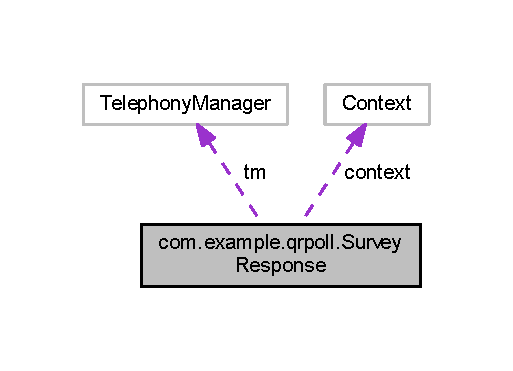
\includegraphics[width=246pt]{classcom_1_1example_1_1qrpoll_1_1_survey_response__coll__graph}
\end{center}
\end{figure}
\subsection*{Metody publiczne}
\begin{DoxyCompactItemize}
\item 
\hyperlink{classcom_1_1example_1_1qrpoll_1_1_survey_response_a13d182139934cfb2f681515e76628786}{Survey\+Response} ()
\item 
\hyperlink{classcom_1_1example_1_1qrpoll_1_1_survey_response_af1338f35c7aa2f3b1f8b1d90b0c1fa41}{Survey\+Response} (Context \hyperlink{classcom_1_1example_1_1qrpoll_1_1_survey_response_a9bfbee3bd0f78b7652a590063c6e7073}{context})
\item 
\hyperlink{classcom_1_1example_1_1qrpoll_1_1_survey_response_a5f4e8e2b1847aca4f0ea56c2c7e6ae46}{Survey\+Response} (Telephony\+Manager \hyperlink{classcom_1_1example_1_1qrpoll_1_1_survey_response_ad4ac570c04a756ac4eaa8622186d5933}{tm})
\item 
void \hyperlink{classcom_1_1example_1_1qrpoll_1_1_survey_response_a7c51f0ae34b99c47669f8ea210c9f214}{set\+Context} (Context \hyperlink{classcom_1_1example_1_1qrpoll_1_1_survey_response_a9bfbee3bd0f78b7652a590063c6e7073}{context})
\item 
void \hyperlink{classcom_1_1example_1_1qrpoll_1_1_survey_response_a8513757cb70751abd35ecd4ca292362e}{set\+Tm} ()
\item 
String \hyperlink{classcom_1_1example_1_1qrpoll_1_1_survey_response_ab06ccbc70c50e72eb089134884f1e6ac}{get\+Imei} ()
\item 
String \hyperlink{classcom_1_1example_1_1qrpoll_1_1_survey_response_a5edce8d8944d575ec23b7f567419cd01}{get\+Sim\+Id} ()
\item 
String \hyperlink{classcom_1_1example_1_1qrpoll_1_1_survey_response_a9adfd3c055deca07bf913d65a85c7bad}{create\+Id\+To\+Send} ()
\end{DoxyCompactItemize}
\subsection*{Atrybuty prywatne}
\begin{DoxyCompactItemize}
\item 
Telephony\+Manager \hyperlink{classcom_1_1example_1_1qrpoll_1_1_survey_response_ad4ac570c04a756ac4eaa8622186d5933}{tm}
\item 
Context \hyperlink{classcom_1_1example_1_1qrpoll_1_1_survey_response_a9bfbee3bd0f78b7652a590063c6e7073}{context}
\end{DoxyCompactItemize}


\subsection{Opis szczegółowy}
Klasa do pobierania I\+M\+E\+I i wysylania go na serwer (do przetestowania, moj tel z androidem sie zepsul wiec nie mam jak dobrze przetestowac tego \begin{DoxyAuthor}{Autor}
Sliwka 
\end{DoxyAuthor}


Definicja w linii 22 pliku Survey\+Response.\+java.



\subsection{Dokumentacja konstruktora i destruktora}
\hypertarget{classcom_1_1example_1_1qrpoll_1_1_survey_response_a13d182139934cfb2f681515e76628786}{\index{com\+::example\+::qrpoll\+::\+Survey\+Response@{com\+::example\+::qrpoll\+::\+Survey\+Response}!Survey\+Response@{Survey\+Response}}
\index{Survey\+Response@{Survey\+Response}!com\+::example\+::qrpoll\+::\+Survey\+Response@{com\+::example\+::qrpoll\+::\+Survey\+Response}}
\subsubsection[{Survey\+Response}]{\setlength{\rightskip}{0pt plus 5cm}com.\+example.\+qrpoll.\+Survey\+Response.\+Survey\+Response (
\begin{DoxyParamCaption}
{}
\end{DoxyParamCaption}
)}}\label{classcom_1_1example_1_1qrpoll_1_1_survey_response_a13d182139934cfb2f681515e76628786}


Definicja w linii 27 pliku Survey\+Response.\+java.


\begin{DoxyCode}
27 \{   \}
\end{DoxyCode}
\hypertarget{classcom_1_1example_1_1qrpoll_1_1_survey_response_af1338f35c7aa2f3b1f8b1d90b0c1fa41}{\index{com\+::example\+::qrpoll\+::\+Survey\+Response@{com\+::example\+::qrpoll\+::\+Survey\+Response}!Survey\+Response@{Survey\+Response}}
\index{Survey\+Response@{Survey\+Response}!com\+::example\+::qrpoll\+::\+Survey\+Response@{com\+::example\+::qrpoll\+::\+Survey\+Response}}
\subsubsection[{Survey\+Response}]{\setlength{\rightskip}{0pt plus 5cm}com.\+example.\+qrpoll.\+Survey\+Response.\+Survey\+Response (
\begin{DoxyParamCaption}
\item[{Context}]{context}
\end{DoxyParamCaption}
)}}\label{classcom_1_1example_1_1qrpoll_1_1_survey_response_af1338f35c7aa2f3b1f8b1d90b0c1fa41}


Definicja w linii 29 pliku Survey\+Response.\+java.


\begin{DoxyCode}
29                                           \{
30         this.context=\hyperlink{classcom_1_1example_1_1qrpoll_1_1_survey_response_a9bfbee3bd0f78b7652a590063c6e7073}{context};
31         \hyperlink{classcom_1_1example_1_1qrpoll_1_1_survey_response_ad4ac570c04a756ac4eaa8622186d5933}{tm}=(TelephonyManager)\hyperlink{classcom_1_1example_1_1qrpoll_1_1_survey_response_a9bfbee3bd0f78b7652a590063c6e7073}{context}.getSystemService(Context.TELEPHONY\_SERVICE);
32     \}
\end{DoxyCode}
\hypertarget{classcom_1_1example_1_1qrpoll_1_1_survey_response_a5f4e8e2b1847aca4f0ea56c2c7e6ae46}{\index{com\+::example\+::qrpoll\+::\+Survey\+Response@{com\+::example\+::qrpoll\+::\+Survey\+Response}!Survey\+Response@{Survey\+Response}}
\index{Survey\+Response@{Survey\+Response}!com\+::example\+::qrpoll\+::\+Survey\+Response@{com\+::example\+::qrpoll\+::\+Survey\+Response}}
\subsubsection[{Survey\+Response}]{\setlength{\rightskip}{0pt plus 5cm}com.\+example.\+qrpoll.\+Survey\+Response.\+Survey\+Response (
\begin{DoxyParamCaption}
\item[{Telephony\+Manager}]{tm}
\end{DoxyParamCaption}
)}}\label{classcom_1_1example_1_1qrpoll_1_1_survey_response_a5f4e8e2b1847aca4f0ea56c2c7e6ae46}


Definicja w linii 34 pliku Survey\+Response.\+java.


\begin{DoxyCode}
34                                               \{
35         this.tm=\hyperlink{classcom_1_1example_1_1qrpoll_1_1_survey_response_ad4ac570c04a756ac4eaa8622186d5933}{tm};
36     \}
\end{DoxyCode}


\subsection{Dokumentacja funkcji składowych}
\hypertarget{classcom_1_1example_1_1qrpoll_1_1_survey_response_a9adfd3c055deca07bf913d65a85c7bad}{\index{com\+::example\+::qrpoll\+::\+Survey\+Response@{com\+::example\+::qrpoll\+::\+Survey\+Response}!create\+Id\+To\+Send@{create\+Id\+To\+Send}}
\index{create\+Id\+To\+Send@{create\+Id\+To\+Send}!com\+::example\+::qrpoll\+::\+Survey\+Response@{com\+::example\+::qrpoll\+::\+Survey\+Response}}
\subsubsection[{create\+Id\+To\+Send}]{\setlength{\rightskip}{0pt plus 5cm}String com.\+example.\+qrpoll.\+Survey\+Response.\+create\+Id\+To\+Send (
\begin{DoxyParamCaption}
{}
\end{DoxyParamCaption}
)}}\label{classcom_1_1example_1_1qrpoll_1_1_survey_response_a9adfd3c055deca07bf913d65a85c7bad}
Tworzy id zlozone z 8 znakow imei i 8 znakow nr karty sim \begin{DoxyReturn}{Zwraca}

\end{DoxyReturn}


Definicja w linii 66 pliku Survey\+Response.\+java.


\begin{DoxyCode}
66                                   \{
67         String imei=\hyperlink{classcom_1_1example_1_1qrpoll_1_1_survey_response_ab06ccbc70c50e72eb089134884f1e6ac}{getImei}().substring(0, 8);
68         String sim=\hyperlink{classcom_1_1example_1_1qrpoll_1_1_survey_response_a5edce8d8944d575ec23b7f567419cd01}{getSimId}().substring(0, 8);
69         \textcolor{keywordflow}{return} imei+sim;
70     \}
\end{DoxyCode}
\hypertarget{classcom_1_1example_1_1qrpoll_1_1_survey_response_ab06ccbc70c50e72eb089134884f1e6ac}{\index{com\+::example\+::qrpoll\+::\+Survey\+Response@{com\+::example\+::qrpoll\+::\+Survey\+Response}!get\+Imei@{get\+Imei}}
\index{get\+Imei@{get\+Imei}!com\+::example\+::qrpoll\+::\+Survey\+Response@{com\+::example\+::qrpoll\+::\+Survey\+Response}}
\subsubsection[{get\+Imei}]{\setlength{\rightskip}{0pt plus 5cm}String com.\+example.\+qrpoll.\+Survey\+Response.\+get\+Imei (
\begin{DoxyParamCaption}
{}
\end{DoxyParamCaption}
)}}\label{classcom_1_1example_1_1qrpoll_1_1_survey_response_ab06ccbc70c50e72eb089134884f1e6ac}
zwraca nr imei telefonu \begin{DoxyReturn}{Zwraca}

\end{DoxyReturn}


Definicja w linii 51 pliku Survey\+Response.\+java.


\begin{DoxyCode}
51                            \{
52         \textcolor{keywordflow}{return} tm.getDeviceId();
53     \}
\end{DoxyCode}
\hypertarget{classcom_1_1example_1_1qrpoll_1_1_survey_response_a5edce8d8944d575ec23b7f567419cd01}{\index{com\+::example\+::qrpoll\+::\+Survey\+Response@{com\+::example\+::qrpoll\+::\+Survey\+Response}!get\+Sim\+Id@{get\+Sim\+Id}}
\index{get\+Sim\+Id@{get\+Sim\+Id}!com\+::example\+::qrpoll\+::\+Survey\+Response@{com\+::example\+::qrpoll\+::\+Survey\+Response}}
\subsubsection[{get\+Sim\+Id}]{\setlength{\rightskip}{0pt plus 5cm}String com.\+example.\+qrpoll.\+Survey\+Response.\+get\+Sim\+Id (
\begin{DoxyParamCaption}
{}
\end{DoxyParamCaption}
)}}\label{classcom_1_1example_1_1qrpoll_1_1_survey_response_a5edce8d8944d575ec23b7f567419cd01}
zwraca identyfikator karty sim \begin{DoxyReturn}{Zwraca}

\end{DoxyReturn}


Definicja w linii 59 pliku Survey\+Response.\+java.


\begin{DoxyCode}
59                             \{
60         \textcolor{keywordflow}{return} tm.getSimSerialNumber();
61     \}
\end{DoxyCode}
\hypertarget{classcom_1_1example_1_1qrpoll_1_1_survey_response_a7c51f0ae34b99c47669f8ea210c9f214}{\index{com\+::example\+::qrpoll\+::\+Survey\+Response@{com\+::example\+::qrpoll\+::\+Survey\+Response}!set\+Context@{set\+Context}}
\index{set\+Context@{set\+Context}!com\+::example\+::qrpoll\+::\+Survey\+Response@{com\+::example\+::qrpoll\+::\+Survey\+Response}}
\subsubsection[{set\+Context}]{\setlength{\rightskip}{0pt plus 5cm}void com.\+example.\+qrpoll.\+Survey\+Response.\+set\+Context (
\begin{DoxyParamCaption}
\item[{Context}]{context}
\end{DoxyParamCaption}
)}}\label{classcom_1_1example_1_1qrpoll_1_1_survey_response_a7c51f0ae34b99c47669f8ea210c9f214}


Definicja w linii 38 pliku Survey\+Response.\+java.


\begin{DoxyCode}
38                                            \{
39         this.context=\hyperlink{classcom_1_1example_1_1qrpoll_1_1_survey_response_a9bfbee3bd0f78b7652a590063c6e7073}{context};
40     \}
\end{DoxyCode}
\hypertarget{classcom_1_1example_1_1qrpoll_1_1_survey_response_a8513757cb70751abd35ecd4ca292362e}{\index{com\+::example\+::qrpoll\+::\+Survey\+Response@{com\+::example\+::qrpoll\+::\+Survey\+Response}!set\+Tm@{set\+Tm}}
\index{set\+Tm@{set\+Tm}!com\+::example\+::qrpoll\+::\+Survey\+Response@{com\+::example\+::qrpoll\+::\+Survey\+Response}}
\subsubsection[{set\+Tm}]{\setlength{\rightskip}{0pt plus 5cm}void com.\+example.\+qrpoll.\+Survey\+Response.\+set\+Tm (
\begin{DoxyParamCaption}
{}
\end{DoxyParamCaption}
)}}\label{classcom_1_1example_1_1qrpoll_1_1_survey_response_a8513757cb70751abd35ecd4ca292362e}
ustawia telephony manager 

Definicja w linii 44 pliku Survey\+Response.\+java.


\begin{DoxyCode}
44                        \{
45         \hyperlink{classcom_1_1example_1_1qrpoll_1_1_survey_response_ad4ac570c04a756ac4eaa8622186d5933}{tm}=(TelephonyManager)\hyperlink{classcom_1_1example_1_1qrpoll_1_1_survey_response_a9bfbee3bd0f78b7652a590063c6e7073}{context}.getSystemService(Context.TELEPHONY\_SERVICE);
46     \}
\end{DoxyCode}


\subsection{Dokumentacja atrybutów składowych}
\hypertarget{classcom_1_1example_1_1qrpoll_1_1_survey_response_a9bfbee3bd0f78b7652a590063c6e7073}{\index{com\+::example\+::qrpoll\+::\+Survey\+Response@{com\+::example\+::qrpoll\+::\+Survey\+Response}!context@{context}}
\index{context@{context}!com\+::example\+::qrpoll\+::\+Survey\+Response@{com\+::example\+::qrpoll\+::\+Survey\+Response}}
\subsubsection[{context}]{\setlength{\rightskip}{0pt plus 5cm}Context com.\+example.\+qrpoll.\+Survey\+Response.\+context\hspace{0.3cm}{\ttfamily [private]}}}\label{classcom_1_1example_1_1qrpoll_1_1_survey_response_a9bfbee3bd0f78b7652a590063c6e7073}


Definicja w linii 25 pliku Survey\+Response.\+java.

\hypertarget{classcom_1_1example_1_1qrpoll_1_1_survey_response_ad4ac570c04a756ac4eaa8622186d5933}{\index{com\+::example\+::qrpoll\+::\+Survey\+Response@{com\+::example\+::qrpoll\+::\+Survey\+Response}!tm@{tm}}
\index{tm@{tm}!com\+::example\+::qrpoll\+::\+Survey\+Response@{com\+::example\+::qrpoll\+::\+Survey\+Response}}
\subsubsection[{tm}]{\setlength{\rightskip}{0pt plus 5cm}Telephony\+Manager com.\+example.\+qrpoll.\+Survey\+Response.\+tm\hspace{0.3cm}{\ttfamily [private]}}}\label{classcom_1_1example_1_1qrpoll_1_1_survey_response_ad4ac570c04a756ac4eaa8622186d5933}


Definicja w linii 24 pliku Survey\+Response.\+java.



Dokumentacja dla tej klasy została wygenerowana z pliku\+:\begin{DoxyCompactItemize}
\item 
\hyperlink{_survey_response_8java}{Survey\+Response.\+java}\end{DoxyCompactItemize}

\chapter{Dokumentacja plików}
\hypertarget{_choice_8java}{\section{Dokumentacja pliku Choice.\+java}
\label{_choice_8java}\index{Choice.\+java@{Choice.\+java}}
}
\subsection*{Komponenty}
\begin{DoxyCompactItemize}
\item 
class \hyperlink{classcom_1_1example_1_1qrpoll_1_1_choice}{com.\+example.\+qrpoll.\+Choice}
\end{DoxyCompactItemize}
\subsection*{Pakiety}
\begin{DoxyCompactItemize}
\item 
package \hyperlink{namespacecom_1_1example_1_1qrpoll}{com.\+example.\+qrpoll}
\end{DoxyCompactItemize}

\hypertarget{_exception404_8java}{\section{Dokumentacja pliku Exception404.\+java}
\label{_exception404_8java}\index{Exception404.\+java@{Exception404.\+java}}
}
\subsection*{Komponenty}
\begin{DoxyCompactItemize}
\item 
class \hyperlink{classcom_1_1example_1_1qrpoll_1_1_exception404}{com.\+example.\+qrpoll.\+Exception404}
\end{DoxyCompactItemize}
\subsection*{Pakiety}
\begin{DoxyCompactItemize}
\item 
package \hyperlink{namespacecom_1_1example_1_1qrpoll}{com.\+example.\+qrpoll}
\end{DoxyCompactItemize}

\hypertarget{_expandable_list_adapter_8java}{\section{Dokumentacja pliku Expandable\+List\+Adapter.\+java}
\label{_expandable_list_adapter_8java}\index{Expandable\+List\+Adapter.\+java@{Expandable\+List\+Adapter.\+java}}
}
\subsection*{Komponenty}
\begin{DoxyCompactItemize}
\item 
class \hyperlink{classcom_1_1example_1_1qrpoll_1_1_expandable_list_adapter}{com.\+example.\+qrpoll.\+Expandable\+List\+Adapter}
\item 
class \hyperlink{classcom_1_1example_1_1qrpoll_1_1_expandable_list_adapter_1_1_button_listener}{com.\+example.\+qrpoll.\+Expandable\+List\+Adapter.\+Button\+Listener}
\end{DoxyCompactItemize}
\subsection*{Pakiety}
\begin{DoxyCompactItemize}
\item 
package \hyperlink{namespacecom_1_1example_1_1qrpoll}{com.\+example.\+qrpoll}
\end{DoxyCompactItemize}

\hypertarget{_history_adapter_8java}{\section{Dokumentacja pliku History\+Adapter.\+java}
\label{_history_adapter_8java}\index{History\+Adapter.\+java@{History\+Adapter.\+java}}
}
\subsection*{Komponenty}
\begin{DoxyCompactItemize}
\item 
class \hyperlink{classcom_1_1example_1_1qrpoll_1_1_history_adapter}{com.\+example.\+qrpoll.\+History\+Adapter}
\end{DoxyCompactItemize}
\subsection*{Pakiety}
\begin{DoxyCompactItemize}
\item 
package \hyperlink{namespacecom_1_1example_1_1qrpoll}{com.\+example.\+qrpoll}
\end{DoxyCompactItemize}

\hypertarget{_history_layout_8java}{\section{Dokumentacja pliku History\+Layout.\+java}
\label{_history_layout_8java}\index{History\+Layout.\+java@{History\+Layout.\+java}}
}
\subsection*{Komponenty}
\begin{DoxyCompactItemize}
\item 
class \hyperlink{classcom_1_1example_1_1qrpoll_1_1_history_layout}{com.\+example.\+qrpoll.\+History\+Layout}
\end{DoxyCompactItemize}
\subsection*{Pakiety}
\begin{DoxyCompactItemize}
\item 
package \hyperlink{namespacecom_1_1example_1_1qrpoll}{com.\+example.\+qrpoll}
\end{DoxyCompactItemize}

\hypertarget{_item_8java}{\section{Dokumentacja pliku Item.\+java}
\label{_item_8java}\index{Item.\+java@{Item.\+java}}
}
\subsection*{Komponenty}
\begin{DoxyCompactItemize}
\item 
class \hyperlink{classcom_1_1example_1_1qrpoll_1_1_item}{com.\+example.\+qrpoll.\+Item}
\end{DoxyCompactItemize}
\subsection*{Pakiety}
\begin{DoxyCompactItemize}
\item 
package \hyperlink{namespacecom_1_1example_1_1qrpoll}{com.\+example.\+qrpoll}
\end{DoxyCompactItemize}

\hypertarget{_main_activity_8java}{\section{Dokumentacja pliku Main\+Activity.\+java}
\label{_main_activity_8java}\index{Main\+Activity.\+java@{Main\+Activity.\+java}}
}
\subsection*{Komponenty}
\begin{DoxyCompactItemize}
\item 
class \hyperlink{classcom_1_1example_1_1qrpoll_1_1_main_activity}{com.\+example.\+qrpoll.\+Main\+Activity}
\item 
class \hyperlink{classcom_1_1example_1_1qrpoll_1_1_main_activity_1_1_placeholder_fragment}{com.\+example.\+qrpoll.\+Main\+Activity.\+Placeholder\+Fragment}
\end{DoxyCompactItemize}
\subsection*{Pakiety}
\begin{DoxyCompactItemize}
\item 
package \hyperlink{namespacecom_1_1example_1_1qrpoll}{com.\+example.\+qrpoll}
\end{DoxyCompactItemize}

\hypertarget{_my_http_u_r_l_connection_8java}{\section{Dokumentacja pliku C\+:/\+Users/\+Wodzu/\+Documents/\+Git\+Hub/\+Projekt\+Zespolowy/\+Android Final + dokumentacja/android/qrpoll/src/com/example/qrpoll/\+My\+Http\+U\+R\+L\+Connection.java}
\label{_my_http_u_r_l_connection_8java}\index{C\+:/\+Users/\+Wodzu/\+Documents/\+Git\+Hub/\+Projekt\+Zespolowy/\+Android Final + dokumentacja/android/qrpoll/src/com/example/qrpoll/\+My\+Http\+U\+R\+L\+Connection.\+java@{C\+:/\+Users/\+Wodzu/\+Documents/\+Git\+Hub/\+Projekt\+Zespolowy/\+Android Final + dokumentacja/android/qrpoll/src/com/example/qrpoll/\+My\+Http\+U\+R\+L\+Connection.\+java}}
}
\subsection*{Komponenty}
\begin{DoxyCompactItemize}
\item 
class \hyperlink{classcom_1_1example_1_1qrpoll_1_1_my_http_u_r_l_connection}{com.\+example.\+qrpoll.\+My\+Http\+U\+R\+L\+Connection}
\end{DoxyCompactItemize}
\subsection*{Pakiety}
\begin{DoxyCompactItemize}
\item 
package \hyperlink{namespacecom_1_1example_1_1qrpoll}{com.\+example.\+qrpoll}
\end{DoxyCompactItemize}

\hypertarget{_poll_8java}{\section{Dokumentacja pliku C\+:/\+Users/\+Wodzu/\+Documents/\+Git\+Hub/\+Projekt\+Zespolowy/\+Android Final + dokumentacja/android/qrpoll/src/com/example/qrpoll/\+Poll.java}
\label{_poll_8java}\index{C\+:/\+Users/\+Wodzu/\+Documents/\+Git\+Hub/\+Projekt\+Zespolowy/\+Android Final + dokumentacja/android/qrpoll/src/com/example/qrpoll/\+Poll.\+java@{C\+:/\+Users/\+Wodzu/\+Documents/\+Git\+Hub/\+Projekt\+Zespolowy/\+Android Final + dokumentacja/android/qrpoll/src/com/example/qrpoll/\+Poll.\+java}}
}
\subsection*{Komponenty}
\begin{DoxyCompactItemize}
\item 
class \hyperlink{classcom_1_1example_1_1qrpoll_1_1_poll}{com.\+example.\+qrpoll.\+Poll}
\end{DoxyCompactItemize}
\subsection*{Pakiety}
\begin{DoxyCompactItemize}
\item 
package \hyperlink{namespacecom_1_1example_1_1qrpoll}{com.\+example.\+qrpoll}
\end{DoxyCompactItemize}

\hypertarget{_poll_activity_8java}{\section{Dokumentacja pliku C\+:/\+Users/\+Wodzu/\+Documents/\+Git\+Hub/\+Projekt\+Zespolowy/\+Android Final + dokumentacja/android/qrpoll/src/com/example/qrpoll/\+Poll\+Activity.java}
\label{_poll_activity_8java}\index{C\+:/\+Users/\+Wodzu/\+Documents/\+Git\+Hub/\+Projekt\+Zespolowy/\+Android Final + dokumentacja/android/qrpoll/src/com/example/qrpoll/\+Poll\+Activity.\+java@{C\+:/\+Users/\+Wodzu/\+Documents/\+Git\+Hub/\+Projekt\+Zespolowy/\+Android Final + dokumentacja/android/qrpoll/src/com/example/qrpoll/\+Poll\+Activity.\+java}}
}
\subsection*{Komponenty}
\begin{DoxyCompactItemize}
\item 
class \hyperlink{classcom_1_1example_1_1qrpoll_1_1_poll_activity}{com.\+example.\+qrpoll.\+Poll\+Activity}
\end{DoxyCompactItemize}
\subsection*{Pakiety}
\begin{DoxyCompactItemize}
\item 
package \hyperlink{namespacecom_1_1example_1_1qrpoll}{com.\+example.\+qrpoll}
\end{DoxyCompactItemize}

\hypertarget{_question_8java}{\section{Dokumentacja pliku Question.\+java}
\label{_question_8java}\index{Question.\+java@{Question.\+java}}
}
\subsection*{Komponenty}
\begin{DoxyCompactItemize}
\item 
class \hyperlink{classcom_1_1example_1_1qrpoll_1_1_question}{com.\+example.\+qrpoll.\+Question}
\end{DoxyCompactItemize}
\subsection*{Pakiety}
\begin{DoxyCompactItemize}
\item 
package \hyperlink{namespacecom_1_1example_1_1qrpoll}{com.\+example.\+qrpoll}
\end{DoxyCompactItemize}

\hypertarget{_refresh_8java}{\section{Dokumentacja pliku C\+:/\+Users/\+Wodzu/\+Documents/\+Git\+Hub/\+Projekt\+Zespolowy/\+Android Final + dokumentacja/android/qrpoll/src/com/example/qrpoll/\+Refresh.java}
\label{_refresh_8java}\index{C\+:/\+Users/\+Wodzu/\+Documents/\+Git\+Hub/\+Projekt\+Zespolowy/\+Android Final + dokumentacja/android/qrpoll/src/com/example/qrpoll/\+Refresh.\+java@{C\+:/\+Users/\+Wodzu/\+Documents/\+Git\+Hub/\+Projekt\+Zespolowy/\+Android Final + dokumentacja/android/qrpoll/src/com/example/qrpoll/\+Refresh.\+java}}
}
\subsection*{Komponenty}
\begin{DoxyCompactItemize}
\item 
class \hyperlink{classcom_1_1example_1_1qrpoll_1_1_refresh}{com.\+example.\+qrpoll.\+Refresh}
\end{DoxyCompactItemize}
\subsection*{Pakiety}
\begin{DoxyCompactItemize}
\item 
package \hyperlink{namespacecom_1_1example_1_1qrpoll}{com.\+example.\+qrpoll}
\end{DoxyCompactItemize}

\hypertarget{_sql_handler_8java}{\section{Dokumentacja pliku Sql\+Handler.\+java}
\label{_sql_handler_8java}\index{Sql\+Handler.\+java@{Sql\+Handler.\+java}}
}
\subsection*{Komponenty}
\begin{DoxyCompactItemize}
\item 
class \hyperlink{classcom_1_1example_1_1qrpoll_1_1_sql_handler}{com.\+example.\+qrpoll.\+Sql\+Handler}
\item 
class \hyperlink{classcom_1_1example_1_1qrpoll_1_1_sql_handler_1_1_database_helper}{com.\+example.\+qrpoll.\+Sql\+Handler.\+Database\+Helper}
\end{DoxyCompactItemize}
\subsection*{Pakiety}
\begin{DoxyCompactItemize}
\item 
package \hyperlink{namespacecom_1_1example_1_1qrpoll}{com.\+example.\+qrpoll}
\end{DoxyCompactItemize}

\hypertarget{_survey_response_8java}{\section{Dokumentacja pliku Survey\+Response.\+java}
\label{_survey_response_8java}\index{Survey\+Response.\+java@{Survey\+Response.\+java}}
}
\subsection*{Komponenty}
\begin{DoxyCompactItemize}
\item 
class \hyperlink{classcom_1_1example_1_1qrpoll_1_1_survey_response}{com.\+example.\+qrpoll.\+Survey\+Response}
\end{DoxyCompactItemize}
\subsection*{Pakiety}
\begin{DoxyCompactItemize}
\item 
package \hyperlink{namespacecom_1_1example_1_1qrpoll}{com.\+example.\+qrpoll}
\end{DoxyCompactItemize}

%--- End generated contents ---

% Index
\newpage
\phantomsection
\addcontentsline{toc}{chapter}{Indeks}
\printindex

\end{document}
